%---置入定義檔 ----------------------------------
%--- BOOK 定義檔
\documentclass[12pt, a4paper]{book}
\setlength{\textwidth}{13cm} %設定書面文字寬度
\usepackage{geometry}
 \geometry{
 a4paper,
 right=25mm,
 left=25mm,
 top=25mm,
 bottom=25mm
 }
%\usepackage[left=2.5cm,right=2.5cm,top=2cm,bottom=2cm]{geometry} 
%--- 定義頁眉頁足 -------------------------------
\usepackage{fancyhdr}
\pagestyle{fancy}
\fancyhf{}
\renewcommand{\chaptermark}[1]{\markboth{\thechapter .\ #1}{}} %去除章編號前後的字
\fancyhead[LE]{\thepage \;\; \XeLaTeX 一本書}
\fancyhead[RO]{\leftmark \;\; \thepage }
%\rhead{\ctxff 數學與電腦}
%\cfoot{\thepage}
\renewcommand{\headrulewidth}{1pt} %頁眉下方的橫線

%----- 定義使用的 packages ----------------------
\usepackage{fontspec} 										 
%\usepackage[BoldFont, SlantFont]{xeCJK}		
\usepackage{xeCJK}											
\defaultfontfeatures{Mapping=tex-text} 				% to support TeX conventions like ``---''
\usepackage{xunicode} 								% Unicode support for LaTeX character names (accents, European chars, etc)
\usepackage{xltxtra} 								% Extra customizations for XeLaTeX
\usepackage{amsmath, amssymb}
\usepackage{amsthm}									% theroemstyle 需要使用的套件
\usepackage[sf,small]{titlesec}
\usepackage{enumerate}
\usepackage{graphicx,subfig,float,wrapfig} 		
\usepackage[outercaption]{sidecap} %[options]=[outercaption], [innercaption], [leftcaption], [rightcaption]
\usepackage{array, booktabs}
\usepackage{color, xcolor}
\usepackage{multirow}
\usepackage{longtable}
\usepackage{colortbl}                          				
\usepackage{natbib}									% for Reference
\usepackage{makeidx}									% for Indexing
\usepackage{listings}								%直接從 latex 碼轉換成顯示文字
\usepackage[parfill]{parskip} 						% Activate to begin paragraphs with an empty line rather than an indent
%\usepackage{geometry} 			% See geometry.pdf to learn the layout options. There are lots.
%\usepackage[left=1.5in,right=1in,top=1in,bottom=1in]{geometry} 

%-----------------------------------------------------------------------------------------------------------------------
%\setCJKmainfont
%	[
%		BoldFont=MS Gothic	% 定義粗體的字型(依使用的電腦安裝的字型而定)
%	]
%	{cwTeX Q Ming Medium} 							% 設定中文內文字型
%	{新細明體}	
%\setmainfont{Times New Roman}							% 設定英文內文字型
%\setsansfont{Arial}									% used with {\sffamily ...}
%\setsansfont[Scale=MatchLowercase,Mapping=tex-text]{Gill Sans}
%\setmonofont{Courier New}							% used with {\ttfamily ...}
%\setmonofont[Scale=MatchLowercase]{Andale Mono}
% 其他字型(隨使用的電腦安裝的字型不同,用註解的方式調整(打開或關閉))
% 英文字型
%\newfontfamily{\E}{Calibri}							% 套用在內文中所有的英文字母
%\newfontfamily{\A}{Arial}
%\newfontfamily{\C}[Scale=0.9]{Calibri}
%\newfontfamily{\TT}[Scale=0.8]{Times New Roman}
% 中文字型
%\newCJKfontfamily{\MB}{Microsoft JhengHei UI}	
% 適用在 Mac 與 Win
%\newCJKfontfamily{\SM}[Scale=0.8]{新細明體}			
% 縮小版新細明體
%\newCJKfontfamily{\K}{標楷體}  
%\newCJKfontfamily{\CF}{cwTeX Q Fangsong Medium}	% CwTex 仿宋體
%\newCJKfontfamily{\CB}{cwTeX Q Hei Bold}			% CwTex 粗黑體
%\newCJKfontfamily{\CK}{cwTeX Q Kai Medium}   	% CwTex 楷體
%\newCJKfontfamily{\CM}{cwTeX Q Ming Medium}		% CwTex 明體
%\newCJKfontfamily{\CR}{cwTeX Q Yuan Medium}		% CwTex 圓體                      	% Windows 下的標楷體
%  中英文內文字型設定
\setCJKmainfont							% 設定中文內文字型
	[
%		BoldFont=Microsoft YaHei	    % 定義粗體的字型(Win)
		BoldFont=黑體-繁	    		    % 定義粗體的字型(Mac)
	]
%	{新細明體}						    % 設定中文內文字型(Win)
	{宋體-繁}							% 設定中文內文字型(Mac)	
\setmainfont{Times New Roman}		    % 設定英文內文字型
\setsansfont{Arial}					    % 無襯字字型 used with {\sffamily ...}
%\setsansfont[Scale=MatchLowercase,Mapping=tex-text]{Gill Sans}
\setmonofont{Courier New}			    % 等寬字型 used with {\ttfamily ...}
%\setmonofont[Scale=MatchLowercase]{Andale Mono}
% 其他字型(隨使用的電腦安裝的字型不同,用註解的方式調整(打開或關閉))
% 英文字型
\newfontfamily{\A}{Arial}
\newfontfamily{\C}{Cochin}				
\newfontfamily{\SA}[Scale=0.9]{Arial}
\newfontfamily{\R}{Times New Roman}
\newfontfamily{\ST}[Scale=0.8]{Times New Roman}
% 中文字型
%\newCJKfontfamily{\MB}{微軟正黑體}				    % 等寬及無襯線字體 Win
\newCJKfontfamily{\MB}{黑體-繁}				        % 等寬及無襯線字體 Mac
%\newCJKfontfamily{\SM}[Scale=0.8]{新細明體}	        % 縮小版(Win)
\newCJKfontfamily{\SM}[Scale=0.8]{宋體-繁}	        % 縮小版(Mac)
%\newCJKfontfamily{\K}{標楷體}                	    % Windows下的標楷體
\newCJKfontfamily{\K}{黑體-繁}               	    % Mac下的標楷體
%\newCJKfontfamily{\BB}{Microsoft YaHei}		    % 粗體 Win
\newCJKfontfamily{\BB}{宋體-繁}		                % 粗體 Mac
% 以下為自行安裝的字型:CwTex 組合
%\newCJKfontfamily{\CF}{cwTeX Q Fangsong Medium}	% CwTex 仿宋體
%\newCJKfontfamily{\CB}{cwTeX Q Hei Bold}			% CwTex 粗黑體
%\newCJKfontfamily{\CK}{cwTeX Q Kai Medium}   	    % CwTex 楷體
%\newCJKfontfamily{\CM}{cwTeX Q Ming Medium}		% CwTex 明體
%\newCJKfontfamily{\CR}{cwTeX Q Yuan Medium}		% CwTex 圓體
%--------------------------------------------------------------------------------------
\XeTeXlinebreaklocale "zh"             %這兩行一定要加,中文才能自動換行
\XeTeXlinebreakskip = 0pt plus 1pt     %這兩行一定要加,中文才能自動換行
%---------------------------------------------------------------------------------------
%----- 重新定義的指令 ---------------------------
\newcommand{\cw}{\texttt{cw}\kern-.6pt\TeX}	% 這是 cwTex 的 logo 文字
\newcommand{\imgdir}{/Users/guoyixuan/Documents/NTPU_STAT/images/}				
\renewcommand{\tablename}{表}					% 改變表格標號文字為中文的「表」(預設為 Table)
\renewcommand{\figurename}{圖}				% 改變圖片標號文字為中文的「圖」(預設為 Figure)
%\renewcommand{\figurename}{圖\hspace*{-.5mm}}
%  for Long Report or Book
\renewcommand{\contentsname}{{\MB 目錄}}
\renewcommand\listfigurename{{\MB 圖目錄}}
\renewcommand\listtablename{{\MB 表目錄}}
\renewcommand{\indexname}{{\MB 索引}}
\renewcommand{\bibname}{{\MB 參考文獻}}
%----------COUNTER -----------------------------------------------------------------------------------------------

\theoremstyle{plain}
\newtheorem{de}{Definition}[section]		%definition獨立編號
\newtheorem{thm}{{\MB 定理}}[section]		%theorem 獨立編號,取中文名稱並給予不同字型
\newtheorem{lemma}[thm]{Lemma}			%lemma 與 theorem 共用編號
\newtheorem{ex}{{\E Example}}				%example 獨立編號,不編入小節數字,走流水號。也換個字型。
\newtheorem{cor}{Corollary}[section]		%not used here
\newtheorem{exercise}{EXERCISE}			%not used here
\newtheorem{re}{\emph{Result}}[section]	%not used here
\newtheorem{axiom}{AXIOM}				%not used here
\renewcommand{\proofname}{\bf{Proof}}		%not used here
\newcounter{quiz}						% start a simple and new counter
\setcounter{quiz}{1}						% start to count from 1
%------------------------------------------------------------------------------------------------------------------

\newcommand{\loflabel}{圖} % 圖目錄出現 圖 x.x 的「圖」字
\newcommand{\lotlabel}{表}  % 表目錄出現 表 x.x 的「表」字

\parindent=0pt
\setcounter{tocdepth}{0}

%--- 其他定義 ----------------------------------
% 定義章節標題的字型、大小
\titleformat{\chapter}[display]{\raggedright\LARGE\MB}{\MB 第\ \thechapter\ 章}{0.2cm}{}
% \titleformat{\chapter}{\center\LARGE\MB}{\MB 第\ \thechapter\ 章、}{0.2cm}{}
% \titleformat{\chapter}{\centering\Huge\bfseries}{第\,\thechapter\,章}{1em}{}
%\titleformat{\chapter}[hang]{\centering\LARGE\sf}{\MB 第~\thesection~章}{0.2cm}{}%控制章的字體
%\titleformat{\section}[hang]{\Large\sf}{\MB 第~\thesection~節}{0.2cm}{}%控制章的字體
%\titleformat{\subsection}[hang]{\centering\Large\sf}{\MB 第~\thesubsection~節}{0.2cm}{}%控制節的字體
\titleformat*{\section}{\normalfont\Large\bfseries\MB}
\titleformat*{\subsection}{\normalfont\large\bfseries\MB}
\titleformat*{\subsubsection}{\normalfont\large\bfseries\MB}


\definecolor{slight}{gray}{0.9}				% 設定顏色
\definecolor{airforceblue}{rgb}{0.36, 0.54, 0.66} % color Table: http://latexcolor.com
\definecolor{arylideyellow}{rgb}{0.91, 0.84, 0.42}
\definecolor{babyblue}{rgb}{0.54, 0.81, 0.94}
\definecolor{cadmiumred}{rgb}{0.89, 0.0, 0.13}
\definecolor{coolblack}{rgb}{0.0, 0.18, 0.39}
\definecolor{beaublue}{rgb}{0.74, 0.83, 0.9}
\definecolor{beige}{rgb}{0.96, 0.96, 0.86}
\definecolor{bisque}{rgb}{1.0, 0.89, 0.77}
\definecolor{gray(x11gray)}{rgb}{0.75, 0.75, 0.75}
\definecolor{limegreen}{rgb}{0.2, 0.8, 0.2}
\definecolor{splashedwhite}{rgb}{1.0, 0.99, 1.0}

%--------------------------------------------------------------------------------------------------------------------------------------------
% 映出程式碼 \begin{lstlisting}
\lstset
{	language=[LaTeX]TeX,
    breaklines=true,
    %basicstyle=\tt\scriptsize,
    basicstyle=\tt\normalsize,
    keywordstyle=\color{blue},
    identifierstyle=\color{black},
    commentstyle=\color{limegreen}\itshape,
    stringstyle=\rmfamily,
    showstringspaces=false,
    %backgroundcolor=\color{splashedwhite},
    backgroundcolor=\color{slight},
    frame=single,							%default frame=none 
    rulecolor=\color{gray(x11gray)},
    framerule=0.4pt,						%expand outward 
    framesep=3pt,							%expand outward
    xleftmargin=3.4pt,						%to make the frame fits in the text area. 
    xrightmargin=3.4pt,						%to make the frame fits in the text area. 
    tabsize=2								%default :8 only influence the lstlisting and lstinline.
}
%\geometry{a4paper,left=2.5cm,right=2.5cm,top=2cm,bottom=2cm}  					
%\usepackage{wallpaper} %浮水印
%\CenterWallPaper{0.7}{\imgdir{wall_paper.png}}
%\URCornerWallPaper{0.15}{\imgdir mactexlogox5.png}
% 啟動索引製作,(1) 配合 \usepackage{makeidx} 使用,
%                      (2) 在文件 \begin{document} 前加入 \makeindex
%                      (3) 在文件最後要印出索引的地方加入 \printondex
%                      (4) 在文章中欲編入索引的文字後加上 \index{該文字}
%                      (5) 編譯時加入 makeindex 一至兩次
\makeindex 						
%----文件開始-------------------------------------
\begin{document}
%---封面製作 ------------------------------------
\fontsize{36}{30pt}\selectfont
\thispagestyle{empty}

\bigskip\bigskip\bigskip\bigskip
\begin{figure}[h]
    \centering
        \includegraphics[scale=2]{\imgdir XeTex.PNG}
        %封面圖片不是放在graph下面,利用新指令指到正確位置
    \end{figure}

\bigskip\bigskip\bigskip\bigskip

\begin{flushright}
    {\BB 統計應用數學與計算}\\
    \rule{16cm}{0.2pt}\\
    \medskip\hfill \Large {\BB 郭翊萱}%\rule{8mm}{0pt}
    \medskip \par\vspace*{-2pt}\hfill \small\today%\rule{8mm}{0pt}
\end{flushright}

%\begin{figure}[H]
%    \centering
%        \subfloat{
%        \includegraphics[scale=1]{\imgdir miktex.png}}%\hspace{1.4cm}
%        \subfloat{
%        \includegraphics[scale=1]{\imgdir mactexlogox5.png}}	
%    \label{fig:mainpage_parallel}
%\end{figure}
    
\fontsize{12}{22pt}\selectfont

%--- 製作目錄 -----------------------------------
\newpage
\cleardoublepage
\setcounter{tocdepth}{2} % 目錄層次
\pagenumbering{roman}  % 羅馬文頁碼

\tableofcontents
\newpage
\renewcommand{\numberline}[1]{\loflabel~#1\hspace*{1em}}% 圖目錄出現 圖 x.x 的「圖」字
\listoffigures %圖目錄
\newpage
\renewcommand{\numberline}[1]{\lotlabel~#1\hspace*{1em}}% 表目錄出現 表 x.x 的「表」字
\listoftables % 表目錄
\newpage
%--- 放入各章 -----------------------------------
\addcontentsline{toc}{chapter}{序}
\chapter*{序}

統計學在許多人心中或許是一門玄學,它基於機率用合理的猜去做合理的推論,但是人們往往對於如何去猜沒有很清晰的認知,許多人會認為統計學就是一門詐騙術,或在政治中操控民調結果,或在統計新冠肺炎數據時用似是而非的方式來引導人們的認知,而這都是基於對陌生事物的恐懼感。\\

人類往往習慣先看見再相信,而對未知事物的恐懼又會阻撓人類睜開雙眼,但是21世紀的人類最寶貴的資產或許就是想睜眼就能看見,而不似前人頂著狂風摸著黑暗前行,一昧的逃避與拒絕了解只會憑白浪費先人與世界給予我們的饋贈,人的一生短短數十年,了解這個世界的邏輯並熱愛這個世界數十年的人生或許才不會活著而像是沒有活著,當你不能善用這個世界給你的禮物而是閉著雙眼生活的時候。

這本書希望能藉由一個單元又一個單元去慢慢引導讀者對於統計學與數學的認知,希望能逐漸引導人們消彌對數學的恐懼以及對統計學的誤解,這本書將利用程式語言來幫助人們了解統計學這片廣袤的土地,利用各種各樣的模擬實驗來幫助讀者一窺其中的有趣之處。本書將首先介紹這本書的製作方式,即利用 \LaTeX 來協助所有的排版、目錄建立以及書本修訂,希望能幫助讀者未來有機會使用到這個工具時能藉由這本書瞭解大部分常用的指令。

第二章與第三章開始則將利用正當風靡的程式語言 Python 來幫助讀者大致了解一些基本的函數圖形以及 Python 中的套件 Matplotlib 的基本使用方式,並介紹多種統計學的基礎機率分配以及這些分配的基本性質,希望能幫助讀者對分配有一些基本的概念。

第四章到第七章則將為讀者介紹七種常用的機器學習方法,機器學習主要有兩個常見的領域,一個是建立變數間的函數利用函數做選擇題,也就是分類問題,另一種則是預測問題,也就是建立函數來做計算題,本書將介紹基本的七種方法,包含簡單線性迴歸 ( Simple Linear Regression )、加廣迴歸 ( Augmented Regression )、羅吉斯迴歸( Logistic Regression )、線性判別分析 ( Linear Discrimunant Analysis )、二次判別分析 ( Quadratic Discriminant Analysis )、K-近鄰演算法 ( KNN ) 以及深度學習領域的類神經網路模型 ( ANN ),並利用統計模擬的方式一一建立模擬資料來檢視這些方法的訓練誤差與測試誤差,希望能幫助讀者對這些方法的理論以及實際應用有更深入的了解,並能在閱讀完本書後能降低一些對未知事物的恐懼甚至嘗試去喜歡它熱愛它,了解這個世界更多一些從來都沒有壞處只有好處,望共勉。

\begin{flushright}
    郭翊萱
    \par\vspace*{-2pt}\hfill 2023年1月於台北大學
\end{flushright}
 	% 序言
%\include{Book_preface_2}	% 序言
\ifodd\count0 \else \thispagestyle{empty}\mbox{}\clearpage\fi % 如果是偶數頁就呈現空白頁
\pagenumbering{arabic} 		% 阿拉伯文頁碼
\setcounter{page}{1} 		% 第一章 從第 1 頁開始
\documentclass[12pt, a4paper]{article} 
\usepackage{fontspec} % Font selection for XeLaTeX; see fontspec.pdf. 

\usepackage{xeCJK}	% 中文使用 XeCJK,利用 \setCJKmainfont 定義中文內文、粗體與斜體的字型
%\usepackage[BoldFont, SlantFont]{xeCJK}
% 中文使用 XeCJK,並模擬粗體與斜體(\textbf{ } \textit{ })

\defaultfontfeatures{Mapping=tex-text} 
% to support TeX conventions like ``---''
\usepackage{xunicode} 
% Unicode support for LaTeX character names(accents, European chars, etc)
\usepackage{xltxtra} 				
% Extra customizations for XeLaTeX
\usepackage{amsmath, amssymb}
\usepackage{enumerate}
\usepackage{graphicx, subfig, float, wrapfig} 
% support the \includegraphics command and options
\usepackage[outercaption]{sidecap} 
%[options]=[outercaption], [innercaption], [leftcaption], [rightcaption]
\usepackage{array, booktabs}
\usepackage{color, xcolor}
% 跨頁的超長表格;lscape是旋轉此類表格的
\usepackage{longtable, lscape}              
% 巨集,使表格加註解更容易(手冊p169)
\usepackage{threeparttable}      
% 讓表格編起來更美的套件(手冊p166),編輯跨列標題重覆的表格(手冊p182)           
\usepackage{multirow, booktabs}             
\usepackage{colortbl}     
% 直接將 latex 碼轉換成顯示文字   
\usepackage{listings}						
% 新段落前加一空行,不使用縮排

\usepackage[parfill]{parskip} 				
% 新段落前加一空行,不使用縮排

\usepackage{geometry} 
% See geometry.pdf to learn the layout options. There are lots.
%\usepackage[left=3in,right=3in,top=2in,bottom=2in]{geometry} 

\usepackage{url}

%.....表格標題註解之巨集套件.....%
% for Reference
\usepackage{natbib}			
% for Indexing				
\usepackage{makeidx}		
% Activate to begin paragraphs with an empty line rather than an indent

%章節設定
\usepackage{titlesec, titletoc,CJKnumb}		


%-----------------------------------------------------------------
%  中英文內文字型設定
%\setCJKmainfont							% 設定中文內文字型
%	[
		%BoldFont=Microsoft YaHei	    %定義粗體的字型(Win)
%		BoldFont=蘋果儷中黑	    		%定義粗體的字型(Mac)
%	]
%	{新細明體}						% 設定中文內文字型(Win)
%	{宋體-繁}							% 設定中文內文字型(Mac)	
%\setmainfont{Times New Roman}		% 設定英文內文字型
%\setsansfont{Arial}					% 無襯字字型 used with {\sffamily ...}
%\setsansfont[Scale=MatchLowercase,Mapping=tex-text]{Gill Sans}
%\setmonofont{Courier New}			% 等寬字型 used with {\ttfamily ...}
%\setmonofont[Scale=MatchLowercase]{Andale Mono}


% 英文字型
%\newfontfamily{\E}{Calibri}				
%\newfontfamily{\A}{Arial}
%\newfontfamily{\C}[Scale=0.9]{Arial}
%\newfontfamily{\R}{Times New Roman}
%\newfontfamily{\TT}[Scale=0.8]{Times New Roman}

% 中文字型
%\newCJKfontfamily{\MB}{微軟正黑體}				% 等寬及無襯線字體 Win
%\newCJKfontfamily{\SM}[Scale=0.8]{新細明體}	% 縮小版(Win)
%\newCJKfontfamily{\K}{標楷體}                	% Windows下的標楷體
%\newCJKfontfamily{\BB}{Microsoft YaHei}		% 粗體 Win
%\newCJKfontfamily{\CF}{cwTeX Q Fangsong Medium}	% CwTex 仿宋體
%\newCJKfontfamily{\CB}{cwTeX Q Hei Bold}			% CwTex 粗黑體
%\newCJKfontfamily{\CK}{cwTeX Q Kai Medium}   	% CwTex 楷體
%\newCJKfontfamily{\CM}{cwTeX Q Ming Medium}		% CwTex 明體
%\newCJKfontfamily{\CR}{cwTeX Q Yuan Medium}		% CwTex 圓體
%----------------------------------------------------------
%  中英文內文字型設定
\setCJKmainfont							% 設定中文內文字型
	[
%		BoldFont=Microsoft YaHei	    % 定義粗體的字型(Win)
		BoldFont=黑體-繁	    		    % 定義粗體的字型(Mac)
	]
%	{新細明體}						    % 設定中文內文字型(Win)
	{宋體-繁}							% 設定中文內文字型(Mac)	
\setmainfont{Times New Roman}		    % 設定英文內文字型
\setsansfont{Arial}					    % 無襯字字型 used with {\sffamily ...}
%\setsansfont[Scale=MatchLowercase,Mapping=tex-text]{Gill Sans}
\setmonofont{Courier New}			    % 等寬字型 used with {\ttfamily ...}
%\setmonofont[Scale=MatchLowercase]{Andale Mono}
% 其他字型(隨使用的電腦安裝的字型不同,用註解的方式調整(打開或關閉))
% 英文字型
\newfontfamily{\A}{Arial}
\newfontfamily{\C}{Cochin}				
\newfontfamily{\SA}[Scale=0.9]{Arial}
\newfontfamily{\R}{Times New Roman}
\newfontfamily{\ST}[Scale=0.8]{Times New Roman}
% 中文字型
%\newCJKfontfamily{\MB}{微軟正黑體}				    % 等寬及無襯線字體 Win
\newCJKfontfamily{\MB}{黑體-繁}				        % 等寬及無襯線字體 Mac
%\newCJKfontfamily{\SM}[Scale=0.8]{新細明體}	        % 縮小版(Win)
\newCJKfontfamily{\SM}[Scale=0.8]{宋體-繁}	        % 縮小版(Mac)
%\newCJKfontfamily{\K}{標楷體}                	    % Windows下的標楷體
\newCJKfontfamily{\K}{黑體-繁}               	    % Mac下的標楷體
%\newCJKfontfamily{\BB}{Microsoft YaHei}		    % 粗體 Win
\newCJKfontfamily{\BB}{宋體-繁}		                % 粗體 Mac
% 以下為自行安裝的字型:CwTex 組合
%\newCJKfontfamily{\CF}{cwTeX Q Fangsong Medium}	% CwTex 仿宋體
%\newCJKfontfamily{\CB}{cwTeX Q Hei Bold}			% CwTex 粗黑體
%\newCJKfontfamily{\CK}{cwTeX Q Kai Medium}   	    % CwTex 楷體
%\newCJKfontfamily{\CM}{cwTeX Q Ming Medium}		% CwTex 明體
%\newCJKfontfamily{\CR}{cwTeX Q Yuan Medium}		% CwTex 圓體
%-------------------------------------------------------------
\XeTeXlinebreaklocale "zh"             		
%這兩行一定要加,中文才能自動換行
\XeTeXlinebreakskip = 0pt plus 1pt     		
%這兩行一定要加,中文才能自動換行
%-----------------------------------------------------------------------------------------------------------------------


\newcommand{\cw}{\texttt{cw}\kern-.6pt\TeX}	% 這是 cwTex 的 logo 文字
\newcommand{\imgdir}{/Users/guoyixuan/Documents/NTPU_STAT/images/}				% 設定圖檔的目錄位置
\renewcommand{\tablename}{表}					% 改變表格標號文字為中文的「表」(預設為 Table)
\renewcommand{\figurename}{圖}				% 改變圖片標號文字為中文的「圖」(預設為 Figure)
\usepackage{booktabs}


% 設定顏色 see color Table: http://latexcolor.com
\usepackage{color}
\definecolor{slight}{gray}{0.9}				
\definecolor{airforceblue}{rgb}{0.36, 0.54, 0.66} 
\definecolor{arylideyellow}{rgb}{0.91, 0.84, 0.42}
\definecolor{babyblue}{rgb}{0.54, 0.81, 0.94}
\definecolor{cadmiumred}{rgb}{0.89, 0.0, 0.13}
\definecolor{coolblack}{rgb}{0.0, 0.18, 0.39}
\definecolor{beaublue}{rgb}{0.74, 0.83, 0.9}
\definecolor{beige}{rgb}{0.96, 0.96, 0.86}
\definecolor{bisque}{rgb}{1.0, 0.89, 0.77}
\definecolor{gray(x11gray)}{rgb}{0.75, 0.75, 0.75}
\definecolor{limegreen}{rgb}{0.2, 0.8, 0.2}
\definecolor{splashedwhite}{rgb}{1.0, 0.99, 1.0}

%---------------------------------------------------------------------
% 映出程式碼 \begin{lstlisting} 的內部設定
\lstset
{	language=[LaTeX]TeX,
    breaklines=true,
    %basicstyle=\tt\scriptsize,
    basicstyle=\tt\normalsize,
    keywordstyle=\color{blue},
    identifierstyle=\color{black},
    commentstyle=\color{limegreen}\itshape,
    stringstyle=\rmfamily,
    showstringspaces=false,
    %backgroundcolor=\color{splashedwhite},
    backgroundcolor=\color{slight},
    frame=single,							%default frame=none 
    rulecolor=\color{gray(x11gray)},
    framerule=0.4pt,							%expand outward 
    framesep=3pt,							%expand outward
    xleftmargin=3.4pt,		%to make the frame fits in the text area. 
    xrightmargin=3.4pt,		%to make the frame fits in the text area. 
    tabsize=2				%default :8 only influence the lstlisting and lstinline.
}

% 映出程式碼 \begin{lstlisting} 的內部設定 for Python codes
%\lstset{language=Python}
%\lstset{frame=lines}
%\lstset{basicstyle=\SCP\normalsize}
%\lstset{keywordstyle=\color{blue}}
%\lstset{commentstyle=\color{airforceblue}\itshape}
%\lstset{backgroundcolor=\color{beige}}

%%%數學式定義定理範例設定%%%
%%theroemstyle 需要使用的套件%%
\usepackage{amsthm}						
\theoremstyle{plain}

%%Definition獨立編號%%
\newtheorem{de}{定義}[section]
%%Theorem獨立編號%%
\newtheorem{thm}{{\MB 定理}}[section]		
%%lemma和theorem共同編號%%
\newtheorem{lemma}[thm]{Lemma}	
%%Example獨立編號%%
\newtheorem{ex}{{\A Example}}			

\newtheorem{cor}{Corollary}[section]		%not used here
\newtheorem{exercise}{EXERCISE}			%not used here
\newtheorem{re}{\emph{Result}}[section]	%not used here
\newtheorem{axiom}{AXIOM}				%not used here
\renewcommand{\proofname}{證明}			%not used here
\newcounter{quiz}						% start a simple and new counter
\setcounter{quiz}{1}						% start to count from 1
   % 使用自己維護的定義檔
%變更章節數字為中文數字
\geometry{a4paper,left=2.5cm,right=2.5cm,top=2cm,bottom=2cm}
\usepackage{fancyhdr}
\pagestyle{fancy}
\fancyhf{}
%\fancyhead[LE,RO]{overleaf}
%\fancyhead[RE,LO]{guides}
%\fancyhead[CE,CO]{\leftmark}
%\fancyhead[LE,RO]{\thepage}


\title{ \LaTeX {\MB 基礎使用教學}}	% 使用設定的字型
\author{{\BB 郭翊萱 711133115}}				% 使用設定的小字體
\date{{\ST 2022.9. }} 			
 
\begin{document}
\maketitle
\fontsize{12}{22pt}\selectfont 
%\chapter{ \XeLaTeX {\MB 基礎應用教學}}

在此文件中,我們將淺度探討 \LaTeX 的一些基本應用,主要包含版面設置、數學式、表格、圖表與各種字形色彩之應用。在首章中,我們將闡述 \LaTeX 如何進行基本的版面設定,並在第二章說明各種數學式的展現,以及如何標記定義、定理與範例。而在第三章中,我們將舉列幾項表格的各種排版方式,並進行各種色彩與粗細的變換。到了最後一章,我們將詳述如何插入各種不同類型的圖片檔,包含jpeg、eps與png,以及多張圖片的各種排版方式。

\section{基本操作}
在建立一個 \LaTeX 文件時,首要的一步便是載入各種 \LaTeX 套件並建立一個屬於自己的設定檔,以便將來之重複使用。為此,本文件將介紹一些基本的版面設定方式,以便持續更新與完善設定檔,並應對未來有可能產生的任何需求。本章將首先介紹一些基本頁面配置方法以及文字的相關設定,其中包含目錄設定、章節設定、各種文字字體與顏色等等。在首節中,本文件將先介紹一些基本頁面配置的方式。

\subsection{頁面配置}
在此小節中,本文件將介紹幾個常用的版面設定方式,首先先介紹最基本的兩個頁面配置方式,其指令如下。
\bigskip
\begin{lstlisting}
  \documentclass[options1]{class}
  \geometry{options2}
\end{lstlisting}


其中
\begin{itemize}
\item[(a)] options1 指定了該文檔的版面設置,如若 options1 為 [11pt, twoside, a4paper],即代表上述指令告訴 \LaTeX 本文檔長寬 A4 紙張相同,文字採雙邊編排(即奇偶頁左右邊距正好相反),基本字體大小是 11pt。
\item[(b)] class 指定了將要被創建的文檔的類型,包含 article (短篇報告與期刊文章) , book (實體書籍) , report (長篇報告) , slides (課程大綱) , beamer (ppt) 等不同文檔類型。
\item[(c)] options2 指定了該文檔上下左右的留白處大小。假設文檔設定 options2 為 [a4paper, left=2.5cm, right=2.5cm, top=2cm, bottom=2cm],即代表 \LaTeX 指定文檔左右空白處寬2.5公分,上下則留白2公分。
\end{itemize}

除了利用  {\A $\backslash$geometry} 進行設定之外,我們也可直接在專屬的設定檔裡面直接利用此套件設定版面,設定方式如下,即直接載入 geometry 包並設定左右留白3公分且上下留白2公分。如有更多其他版面設定需求,可查閱 geometry 包的相關介紹說明。

\bigskip
	\begin{lstlisting}
  \usepackage[left=3in,right=3in,top=2in,bottom=2in]{geometry} 
	\end{lstlisting}
\bigskip

\textbf{頁眉頁腳設定}\\
除了以上的紙張大小、留白等訊息,本文件也將在此介紹基本的頁眉頁腳設定方式。頁眉與頁腳通常位於文件的頂部與尾部,一般文字內容為作者、文章名稱等等。頁眉與頁腳的內容通常相似或互為補充。
\bigskip
\begin{lstlisting}
  \usepackage{fancyhdr}
  \pagestyle{fancy}
\end{lstlisting}

在利用以上指令載入 fancyhdy 包後,則接著加入對頁眉頁腳相關設定的指令,本文件列舉了七個 fancyhdy 包中常見的指令,其內容如下:

\begin{enumerate}
\item {\A $\backslash$fancyhf \{ \}} : 清除頁眉跟頁腳
\item {\A $\backslash$rhead \{ \}} : 在頁眉的右側顯示括號內文字
\item {\A $\backslash$lhead \{ \}} : 在頁眉的左側顯示括號內文字
\item {\A $\backslash$chead \{ \}} : 在頁眉的中間顯示括號內文字
\item {\A $\backslash$rfoot \{ \}} : 在頁腳的左側顯示括號內文字
\item {\A $\backslash$lfoot \{ \}} : 在頁腳的右側顯示括號內文字
\item {\A $\backslash$cfoot \{ \}} : 在頁腳的中間顯示括號內文字
\end{enumerate}

另外,我們亦可改變頁眉頁腳裝飾線的寬度,指令分別如下:
\bigskip
\begin{lstlisting}
  \renewcommand{\headrulewidth}{2pt}
  \renewcommand{\footrulewidth}{2pt}
\end{lstlisting}


\subsubsection{頁碼設置}
在建立\LaTeX 時,可能也會希望頁碼的位置能夠進行改變,因此本文件亦提供一些基本的相關命令,以下即是幾個常用的頁碼設置方式。

\bigskip
\begin{lstlisting}
  \pagestyle{type}
  \thispagestyle{type}
\end{lstlisting}


其中, {\A $\backslash$pagestyle\{type\}} 是同時對所有該文件頁面進行設置,而 {\A $\backslash$thispagestyle\{type\}}  則是僅對當前所在頁面進行頁碼之相關設置。在\LaTeX 中,共默認提供了以下幾種頁面樣式:
\begin{itemize}
\item[$\bullet$] empty: 沒有頁眉跟頁腳。
\item[$\bullet$] plain: 沒有頁眉,頁腳包含一個居中的頁碼。
\item[$\bullet$] heading: 沒有頁腳,頁眉包含章節名字跟頁碼。
\item[$\bullet$] myheadings: 沒有頁腳,頁眉包含頁碼。
\end{itemize}
另外,在 \LaTeX 中亦可利用指令改變頁碼的顯示風格,其中之頁碼風格包含五類,指令與類別如下:

\bigskip
\begin{lstlisting}
  \pagenumbering{style}
\end{lstlisting}

\begin{itemize}
\item[$\bullet$] arabic: 阿拉伯數字
\item[$\bullet$] roman: 小寫羅馬數字
\item[$\bullet$] Roman: 大寫羅馬數字
\item[$\bullet$] alph: 小寫字符形式
\item[$\bullet$] Alph: 大寫字符形式
\end{itemize}

\subsubsection{目錄設置}
介紹完頁碼的設置指令後,本文件接著介紹如何在 \LaTeX 中為文件建立目錄,令 \LaTeX 可以與任何章節或標題的變動進行連動,其基本指令如下:

\bigskip
\begin{lstlisting}
  \tableofcontents
  \newpage
\end{lstlisting}

其中 {\A $\backslash$newpage} 是當希望目錄占滿頁面時接在上面指令後面的指令。接著本文件將陸續介紹關於目錄設定的功能,包含目錄顏色、處理長標題,以及自動令文章中的圖片與表格也生成目錄。

\textbf{目錄顏色}\\
如果載入 hyperref 這個套件,就能令目錄產生顏色,可以更好的告訴顯示此此紅色文字是可以進行點擊跳轉的。
\bigskip
	\begin{lstlisting}
  \usepackage[colorlinks=true]{hyperref}
	\end{lstlisting}

另外,如果在章節前加入星號,即 {\A $\backslash$section*\{introduction\}},即可讓此章節不會顯示在目錄中。

\textbf{長標題處理}\\
當遇到長標題可能超出目錄一行所能顯示的量時, \LaTeX 可以讓文件在目錄顯示短標題而在內文中仍然顯示長標題,如以下指令,在目錄中僅會顯示 \LaTeX 目錄製作,而不會顯示中括號中的長內文。
\bigskip
	\begin{lstlisting}
  \section[\LaTeX 目錄製作]{目錄目錄目錄目錄目錄目錄目錄目錄}
	\end{lstlisting}

另外,如果希望能為圖片與表格生成目錄,則加入指令如下:
\bigskip
	\begin{lstlisting}
  \listoffigures
  \listoftables
	\end{lstlisting}

\subsection{文字設定}
\subsubsection{文字字體與粗細}
以上本文件將直接展現幾種常用的英文與中文字體,以及加粗或斜體等功能。

\textbf{英文字體}

\begin{itemize}
\item[$\bullet$] 一般字體\\
\textnormal{Normal text in Times New Roman font}
    \begin{lstlisting}
  \textnormal{Normal text in Times New Roman font}
	\end{lstlisting}
	
\item[$\bullet$] 加粗字體\\
\textbf{Bold text in Times New Roman font}
	\begin{lstlisting}
  \textbf{Bold text in Times New Roman font}
	\end{lstlisting}
	
\item[$\bullet$] 斜字體\\
\textit{Italic text in Times New Roman font}
    \begin{lstlisting}
  \textit{Italic text in Times New Roman font}
	\end{lstlisting}
	
\item[$\bullet$] 粗體加斜體字\\
\emph{\textbf{My name is Jason.}}
    \begin{lstlisting}
  \emph{\textbf{My name is Jason.}} 
    \end{lstlisting}
    
\item[$\bullet$] 無襯線字體\\
\textsf{Sans-serif text in Tahoma font}
    \begin{lstlisting}
  \textsf{Sans-serif text in Tahoma font}
	\end{lstlisting}
	
\item[$\bullet$] 等寬字體\\
\texttt{Monospace text in Courier New font}
    \begin{lstlisting}
  \texttt{Monospace text in Courier New font}
	\end{lstlisting}
\end{itemize}


\textbf{中文字體}

\begin{itemize}
\item[$\bullet$] 微軟正黑體\\
{\MB 這是微軟正黑體。}
    \begin{lstlisting}
  {\MB 這是微軟正黑體。}
	\end{lstlisting}
\item[$\bullet$] 縮小版新細明體\\
{\SM 這是縮小版新細明體}
	\begin{lstlisting}
  {\SM 這是縮小版新細明體}
	\end{lstlisting}
\item[$\bullet$] 標楷體\\
{\K 這是標楷體}
    \begin{lstlisting}
  {\K 這是標楷體}
	\end{lstlisting}
\item[$\bullet$] 仿宋體\\
{\BB 這是仿宋體}
    \begin{lstlisting}
  {\BB 這是仿宋體}
	\end{lstlisting}
\end{itemize}

\subsubsection{文字顏色與大小}
想要改變顏色的話有幾種不同的方法,本文件將介紹 \LaTeX 兩種常用的改變文字顏色的方法,以及改變字體大小的指令。

\textbf{字體顏色}

\bigskip
\begin{lstlisting}
 \usepackage{color}
 \textcolor{red/blue/green/black/white/cyan/yellow}{text}
 \textcolor[r,g,b]{text}{introduction to machine learning}
\end{lstlisting}

以上即為常見的變更字體顏色的方式,第一種是在 textcolor{ } 中包含定義的顏色以供之後使用,第二種則是建立一個調色盤,其中 r, g, b 代表 red, green, blue 三原色的組合, 取值範圍在 [0,1] 之間。

\textbf{字體大小}

以下表 \ref{tb:basic_1} 介紹了幾種常用的改變字體大小指令。\footnote{以下內容參考自https://blog.csdn.net/yhcwjh/article/details/116516011}


\begin{table}[h] 
\centering
\caption{最基本的表格}\label{tb:basic_1}
\extrarowheight=6pt   %加高行高6pt
\begin{tabular}{lcc}  %取消欄間的直線
\hline
  指令	                  &  對應字號 \\\hline 
  {\A $\backslash$tiny}   & 5pt	\\
  {\A $\backslash$scriptsize}   & 7pt	\\
  {\A $\backslash$footnotesize}   & 8pt	\\
  {\A $\backslash$small}   & 9pt	\\
  {\A $\backslash$normalsize}   & 10pt	\\
  {\A $\backslash$large}   & 12pt	\\
  {\A $\backslash$Large}   & 14.4pt	\\
  {\A $\backslash$LARGE}   & 17.28pt	\\
  {\A $\backslash$huge}   & 20.74pt	\\
  {\A $\backslash$Huge}   & 24.88pt	\\\hline
\end{tabular}
\end{table}


\section{數學符號與方程式}
為了將來能在 \LaTeX 撰寫數學式上流暢無礙,本文件將在第一小節列舉一些常見的數學式作為參考,並在第二小節示範如何利用 \LaTeX 妥善排版定義、定理以及範例題目。輸入數學式時,有兩個地方需要特別注意:\\

\begin{itemize}
\item 隨文數式前後請留一空格,才不會顯得擁擠。
\item 展示數式上下不須多留一空行, \LaTeX\ 會自行調整間距。
\end{itemize}

接著,我們列舉幾項常見的羅馬符號與數學運算記號。

\subsection{常用數學符號}

\subsubsection{常用羅馬符號}

\begin{longtable}{c c c c}
    \caption{羅馬符號}\label{tb:sign} \\
     指令 & 對應字母 & 指令 & 對應字母 \\\hline 
     {\A $\backslash$alpha} & $\alpha$ & {\A $\backslash$upsilon} & $\upsilon$ \\
     {\A $\backslash$beta}  & $\beta$ & {\A $\backslash$Upsilon} & $\Upsilon$ \\
     {\A $\backslash$gamma} & $\gamma$ & {\A $\backslash$Gamma} & $\Gamma$ \\
     {\A $\backslash$delta} & $\delta$	& {\A $\backslash$Delta} & $\Delta$ \\
     {\A $\backslash$epsilon} & $\epsilon$ & {\A $\backslash$xi} & $\xi$ \\
     {\A $\backslash$varepsilon} & $\varepsilon$ & {\A $\backslash$Xi} & $\Xi$ \\
     {\A $\backslash$zeta} & $\zeta$ & {\A $\backslash$pi} & $\pi$ \\
     {\A $\backslash$eta} &  $\eta$ & {\A $\backslash$Pi}  & $\Pi$ \\
     {\A $\backslash$theta} & $\theta$ & {\A $\backslash$rho}  & $\rho$ \\
     {\A $\backslash$vartheta} & $\vartheta$ & {\A $\backslash$sigma} & $\sigma$ \\
     {\A $\backslash$iota} & $\iota$ & {\A $\backslash$Sigma} & $\Sigma$ \\
     {\A $\backslash$kappa} & $\kappa$ & {\A $\backslash$tau} & $\tau$ \\
     {\A $\backslash$lambda} & $\lambda$ & {\A $\backslash$Lambda} & $\Lambda$\\ 
     {\A $\backslash$mu} & $\mu$ & {\A $\backslash$phi} & $\phi$ \\
     {\A $\backslash$nu} & $\nu$ & {\A $\backslash$Phi} & $\Phi$ \\\hline
\end{longtable}

\subsubsection{常用數學運算符號}
\begin{longtable}{c c c c}
    \caption{數學運算符號}\label{tb:sign} \\
     指令 & 對應字母 & 指令 & 對應字母 \\\hline 
     {\A $\backslash$pm} & $\pm$ & {\A $\backslash$mp} & $\mp$ \\
     {\A $\backslash$ast}  & $\ast$ & {\A $\backslash$star} & $\star$ \\
     {\A $\backslash$cdot} & $\cdot$ & {\A $\backslash$cap} & $\cap$ \\
     {\A $\backslash$oplus} & $\oplus$	& {\A $\backslash$ominus} & $\ominus$ \\
     {\A $\backslash$sqcup} & $\sqcup$ & {\A $\backslash$wr} & $\wr$ \\
     {\A $\backslash$vee} & $\vee$ & {\A $\backslash$diamond} & $\diamond$ \\
     {\A $\backslash$triangleleft} & $\triangleleft$ & {\A $\backslash$triangleright} & $\triangleright$ \\
     {\A $\backslash$dagger} &  $\dagger$ & {\A $\backslash$ddagger}  & $\ddagger$ \\
     {\A $\backslash$times} & $\times$ & {\A $\backslash$div}  & $\div$ \\
     {\A $\backslash$circ} & $\circ$ & {\A $\backslash$bullet} & $\bullet$ \\
     {\A $\backslash$cup} & $\cup$ & {\A $\backslash$amalg} & $\amalg$ \\
     {\A $\backslash$otimes} & $\otimes$ & {\A $\backslash$sqcap} & $\sqcap$ \\
     {\A $\backslash$wedge} & $\wedge$ & {\A $\backslash$setminus} & $\setminus$\\ 
     {\A $\backslash$bigtriangleup} & $\bigtriangleup$ & {\A $\backslash$bigtriangledown} & $\bigtriangledown$ \\
     {\A $\backslash$odot} & $\odot$ & {\A $\backslash$bigcirc} & $\bigcirc$ \\\hline
\end{longtable}

\subsubsection{常用數學關係符號}
\begin{longtable}{c c c c}
    \caption{數學運算符號}\label{tb:sign} \\
     指令 & 對應字母 & 指令 & 對應字母 \\\hline 
     {\A $\backslash$leq} & $\leq$ & {\A $\backslash$geq} & $\geq$ \\
     {\A $\backslash$succeq}  & $\succeq$ & {\A $\backslash$prec} & $\prec$ \\
     {\A $\backslash$gg} & $\gg$	& {\A $\backslash$ll} & $\ll$ \\
     {\A $\backslash$subset} & $\subset$ & {\A $\backslash$subseteq} & $\subseteq$ \\
     {\A $\backslash$supset} & $\supset$ & {\A $\backslash$supseteq} & $\supseteq$ \\
     {\A $\backslash$ni} & $\ni$ & {\A $\backslash$in} & $\in$ \\
     {\A $\backslash$dashv} &  $\dashv$ & {\A $\backslash$vdash}  & $\vdash$ \\
     {\A $\backslash$sim} & $\sim$ & {\A $\backslash$simeq}  & $\simeq$ \\
     {\A $\backslash$cong} & $\cong$ & {\A $\backslash$neq} & $\neq$ \\
     {\A $\backslash$doteq} & $\doteq$ & {\A $\backslash$propto} & $\propto$ \\
     {\A $\backslash$perp} & $\perp$ & {\A $\backslash$models} & $\models$ \\
     {\A $\backslash$mid} & $\mid$ & {\A $\backslash$parallel} & $\parallel$ \\\hline
\end{longtable}


\subsubsection{其他常用數學符號}
\begin{longtable}{c c c c}
    \caption{數學運算符號}\label{tb:sign} \\
     指令 & 對應字母 & 指令 & 對應字母 \\\hline 
     {\A $\backslash$leftarrow} & $\leftarrow$ & {\A $\backslash$Longleftrightarrow	} & $\Longleftrightarrow$ \\
     {\A $\backslash$Leftarrow}  & $\Leftarrow$ & {\A $\backslash$longmapsto} & $\longmapsto$ \\
     {\A $\backslash$rightarrow} & $\rightarrow$	& {\A $\backslash$hookrightarrow} & $\hookrightarrow$ \\
     {\A $\backslash$Rightarrow} & $\Rightarrow$ & {\A $\backslash$rightharpoonup} & $\rightharpoonup$ \\
     {\A $\backslash$leftrightarrow} & $\leftrightarrow$ & {\A $\backslash$rightharpoondown} & $\rightharpoondown$ \\
     {\A $\backslash$Leftrightarrow} & $\Leftrightarrow$ & {\A $\backslash$mapsto} & $\mapsto$ \\
     {\A $\backslash$uparrow} &  $\uparrow$ & {\A $\backslash$hookleftarrow}  & $\hookleftarrow$ \\
     {\A $\backslash$Uparrow} & $\Uparrow$ & {\A $\backslash$simeq}  & $\simeq$ \\
     {\A $\backslash$leftharpoonup} & $\leftharpoonup$ & {\A $\backslash$downarrow} & $\downarrow$ \\
     {\A $\backslash$leftharpoondown} & $\leftharpoondown$ & {\A $\backslash$Downarrow} & $\Downarrow$ \\
     {\A $\backslash$rightleftharpoons} & $\rightleftharpoons$ & {\A $\backslash$updownarrow} & $\updownarrow$ \\
     {\A $\backslash$longleftarrow} & $\longleftarrow$ & {\A $\backslash$Updownarrow} & $\Updownarrow$ \\
     {\A $\backslash$Longleftarrow} & $\Longleftarrow$ & {\A $\backslash$nearrow} & $\nearrow$ \\
     {\A $\backslash$longrightarrow} & $\longrightarrow$ & {\A $\backslash$Updownarrow} & $\Updownarrow$ \\
     {\A $\backslash$searrow} & $\searrow$ & {\A $\backslash$Updownarrow} & $\Updownarrow$ \\
     {\A $\backslash$Longrightarrow} & $\Longrightarrow$ & {\A $\backslash$swarrow} & $\swarrow$ \\
     {\A $\backslash$longleftrightarrow} & $\longleftrightarrow$ & {\A $\backslash$nwarrow} & $\nwarrow$ \\\hline
\end{longtable}

\subsubsection{其他常用數學運算符號}
\begin{longtable}{c c c c}
    \caption{數學運算符號}\label{tb:sign} \\
     指令 & 對應字母 & 指令 & 對應字母 \\\hline 
     {\A $\backslash$sum} & $\sum$ & {\A $\backslash$bigcap} & $\bigcap$ \\
     {\A $\backslash$bigodot}  & $\bigodot$ & {\A $\backslash$prod} & $\prod$ \\
     {\A $\backslash$bigcup} & $\bigcup$ & {\A $\backslash$bigotimes} & $\bigotimes$ \\
     {\A $\backslash$coprod} & $\coprod$ & {\A $\backslash$bigoplus} & $\bigoplus$ \\
     {\A $\backslash$int} & $\int$ & {\A $\backslash$bigvee} & $\bigvee$ \\
     {\A $\backslash$biguplus} & $\biguplus$ & {\A $\backslash$oint} & $\oint$ \\
     {\A $\backslash$bigwedge} &  $\bigwedge$ &   &    \\\hline
\end{longtable}

以上介紹了幾種常用的改變字體大小指令,其中一些應用將在下面進行示例。

\subsection{函數}

\begin{itemize}
\item[$\bullet$] 機率分配函數
$$f(x)={n\choose x}p^x(1-p)^{1-x}, \;\; x=0,1,2,\cdots,n$$ 
$$f(x)=\frac{e^{-\lambda}\lambda^x}{x!}, \;\;  x=0,1,2,\cdots$$ 
$$f(x)=\frac{1}{\Gamma(\alpha)\beta^\alpha}x^{\alpha-1}e^{-\frac{x}{\beta}}, \;\; x\geq 0$$
$$f(x)=\frac{1}{\sigma\sqrt{2\pi}}e^{-\frac{(x-\mu)^2}{2\sigma^2}}, \;\;  -\infty < x < \infty $$

\item[$\bullet$] 積分函數
  \begin{equation}\label{eq:gamma}%.................label後的名稱自訂,代表該方程式
  \int^\infty_0 x^{\alpha-1}e^{-\lambda x} dx = \frac{\Gamma(\alpha)}{\lambda^{\alpha}}
  \end{equation}

方程式  (\ref{eq:gamma}) 是廣義 $\Gamma$ 積分。

\item[$\bullet$] 開立方根
$$f(x)=\sqrt[3]{\frac {\displaystyle 4-x^{3}}{\displaystyle 1+x^{2}}}$$

\item[$\bullet$] 極限與微分
$$f'(x)=\frac{df(x)}{dx}=\lim_{h\rightarrow 0}\left(\frac{f(x+h)-f(x)}{h}\right)$$

\end{itemize}


\subsection{聯立方程式}

以下介紹幾種常用的聯立方程式。

\begin{enumerate}

    \item 排列整齊的符號:
        $$ \begin{array}{clr}\\
            a+b+c   & m+n 	& xy \\
            a+b     & p+n 	& yz \\
            b+c     & m-n 	& xz
        \end{array} $$

    \item 等號對齊的函數組合(不編號)
        \begin{eqnarray*}
          b_1 &=& d_1+c_1 \\
          a_2 &=& c_2+e_2
        \end{eqnarray*}

    \item 等號對齊的函數組合(編號在最後一行),如式 (\ref{eq:eqnarray_last})
        \begin{eqnarray}\label{eq:eqnarray_last}
\nonumber b_1 &=& d_1+c_1 \\
          a_2 &=& c_2+e_2
        \end{eqnarray}

    \item 使用套件 {\A amsmath} 的指令 {\A align}(控制編號在第一行),如式 (\ref{eq:eqnarray_first})
        \begin{align} 
            b_1 &= d_1+c_1 \label{eq:eqnarray_first}\\
            a_2 &= c_2+e_2 \notag
        \end{align}

    \item 兩組數學式分別對齊且同時編號,如式 (\ref{eq:eqnarray_both1})與式(\ref{eq:eqnarray_both2})
    \begin{align}
        \alpha_1 &= \beta_1+\gamma_1+\delta_1, &a_1 &= b_1+c_1 \label{eq:eqnarray_both1}\\
        \alpha_2 &= \beta_2+\gamma_2+\delta_2, &a_2 &= b_2+c_2 \label{eq:eqnarray_both2}
    \end{align}

    \item 編號在中間({\A split} 指令環境),如式 (\ref{eq:split})
        \begin{equation} 
            \begin{split} \label{eq:split}
                \alpha_1 &= \beta_1+\gamma_1\\
                \alpha_2 &= \beta_2+\gamma_2
            \end{split}
        \end{equation}
    \item 只是居中對齊的數學式組(環境指令 {\A gather})
        \begin{gather}
        \alpha_1 + \beta_1\notag\\
        \alpha_2 + \beta_2 + \gamma_2\notag
        \end{gather}

    \item 長數學式的表達(注意第二行加號的位置),如式 (\ref{eq:longmath})
        \begin{align}\label{eq:longmath}
            y  	&= x_1 + x_2 + x_3 \notag\\
                	&\quad + x_4 + x_5
        \end{align}
        
    \item 聯立方程式 (不加編號)
     \[ \rho_k=Corr(Y_t,Y_{t-k})=\frac{\gamma_k}{\gamma_0}=\begin{cases}
 		1      &\text{if k=0}\\  
 		\frac{\theta}{1+\theta^{2}}      &\text{if k=1}\\  
 		0      &\text{if k $\geq$ 2}\\  
 	\end{cases}
    \]
    
    \item 聯立方程式 (加編號),如式 (\ref{eq:equation2})
    \begin{equation}\label{eq:equation2}
      Y_t=\begin{cases}
 	   X_t      &\text{for t odd }\\  
 	   X_t+3       &\text{for t even}
    \end{cases}
    \end{equation}
    
    \item 進階聯立方程式 (加編號),如式 (\ref{eq:equationnn})
    \begin{equation}\label{eq:equationnn}
    Cov(Y_t,Y_{t-k})=\begin{cases}
 		Cov(X_t,X_{t-k}+3)      &\text{if t odd, k odd}\\  
 		Cov(X_t,X_{t-k})       &\text{if t odd, k even}\\  
 		Cov(X_t+3,X_{t-k})      &\text{if t even, k odd}\\
 		Cov(X_t+3,X_{t-k}+3)      &\text{if t even, k even}\\         
 	\end{cases}=Cov(X_t,X_{t-k})
 	\end{equation}
    
    \item 進階聯立方程式
    \begin{equation} 
    E(Y_t)=\begin{cases}
 		E(X_t)      &\text{if t odd}\\  
 		E(X_t+3)       &\text{if t even}\\          
 	\end{cases}=\begin{cases}
 	\mu      &\text{if t odd}\\  
 	\mu+3      &\text{if t even}\\  
    \end{cases}
    \end{equation}
    
\end{enumerate}

\subsection{矩陣}

\begin{enumerate}
  \item 左右方框括號的使用及各直行的對齊方式:
 
        $$ A = \left[
            \begin{array}{clr}
                a+b & mnop  & xy \\
                a+b & pn    & yz \\
                b+c & mp    & xyz
            \end{array} \right] $$

  \item 左右圓框刮號的使用及各式點狀:
        $$ A=\left(
            \begin{array}{cccc}
                a_{11} 	& a_{12} & \cdots 	& a_{1n}\\
                a_{21} 	& a_{22} & \cdots 	& a_{2n}\\
                \vdots 	& \vdots & \ddots	& \vdots\\
                a_{n1} 	& a_{n2} & \cdots 	& a_{nn}
            \end{array} \right) $$

  \item 複雜矩陣:
  \[
  M=\begin{bmatrix}
  	Cov(Y_1,Y_1) & Cov(Y_1,Y_2) & \dots & Cov(Y_1,Y_n)\\
  	Cov(Y_2,Y_1) & Cov(Y_2,Y_2) & \dots & Cov(Y_2,Y_n)\\
  	\vdots & \vdots & & \vdots \\
  	Cov(Y_n,Y_1) & Cov(Y_n,Y_2) & \dots & Cov(Y_n,Y_n)
  \end{bmatrix}_{n \times n}
  \]
  \[
  = \begin{bmatrix}
  	\gamma_0 & \gamma_1 & \dots & \gamma_n\\  
  	\gamma_1 & \gamma_0 & \ddots & \vdots \\  
  	\vdots & \ddots & \ddots & \gamma_1 \\  
  	\gamma_{n-1} & \dots & \gamma_1 & \gamma_0
  \end{bmatrix}_{n \times n}
  \]
 \newpage
 \item 巨大矩陣\\
  \begin{center}
  \rotatebox{90}{$
(I-N)^{-1}=\bordermatrix{~ & (0,0) & (1,0) & (2,0) & (3,0) & (4,0) & (5,0) & (6,0) & (7,0) & (8,0) & (9,0) & (10,0) & (11,0)  \cr
(0,0) & 1 & 11 & 55 & 165 & 330 & 462 & 462 & 330 & 165 & 55 & 11 & 1  \cr 
(1,0) & 0 & 11 & 55 & 165 & 330 & 462 & 462 & 330 & 165 & 55 & 11 & 1  \cr 
(2,0) & 0 & 11 & \frac{121}{2} & \frac{363}{2} & 363 & \frac{2541}{5} & \frac{2541}{5} & 363 & \frac{363}{2} & \frac{121}{2} & \frac{121}{10} & \frac{11}{10}  \cr  
(3,0) & 0 & 11 & \frac{121}{2} & \frac{1111}{6} & \frac{1111}{3} & \frac{7777}{15} & \frac{7777}{15}& \frac{1111}{3} & \frac{1111}{6} & \frac{1111}{18} & \frac{1111}{90} & \frac{101}{90}   \cr  
(4,0) & 0 & 11 & \frac{121}{2} & \frac{1111}{6} & \frac{4477}{12} & \frac{31339}{60} & \frac{31339}{60} & \frac{4477}{12} & \frac{4477}{24} & \frac{4477}{72} & \frac{4477}{360} & \frac{407}{360}  \cr  
(5,0) & 0 & 11 & \frac{121}{2} & \frac{1111}{6} & \frac{4477}{12} & \frac{31471}{60} & \frac{31471}{60} & \frac{31471}{84} & \frac{31471}{168} & \frac{31471}{504} & \frac{31471}{2520} & \frac{2861}{60}  \cr  
(6,0) & 0 & 11 & \frac{121}{2} & \frac{1111}{6} & \frac{4477}{12} & \frac{31471}{60} & \frac{10527}{20} & \frac{10527}{28} & \frac{10527}{56} & \frac{3509}{56} & \frac{3509}{280} & \frac{319}{280}  \cr  
(7,0) & 0 & 11 & \frac{121}{2} & \frac{1111}{6} & \frac{4477}{12} & \frac{31471}{60} & \frac{10527}{20} & \frac{10527}{28} & \frac{10571}{56} & \frac{10571}{168} & \frac{10571}{840} & \frac{961}{840}  \cr  
(8,0) & 0 & 11 & \frac{121}{2} & \frac{1111}{6} & \frac{4477}{12} & \frac{31471}{60} & \frac{10527}{20} & \frac{10527}{28} & \frac{1331}{7} & \frac{1331}{21} & \frac{1331}{105} & \frac{121}{105}  \cr  
(9,0) & 0 & 11 & \frac{121}{2} & \frac{1111}{6} & \frac{4477}{12} & \frac{31471}{60} & \frac{10527}{20} & \frac{10527}{28} & \frac{1331}{7} & \frac{4070}{63} & \frac{814}{63} & \frac{74}{63} \cr  
(10,0) & 0 & 11 & \frac{121}{2} & \frac{1111}{6} & \frac{4477}{12} & \frac{31471}{60} & \frac{10527}{20} & \frac{10571}{28} & \frac{1331}{7} & \frac{4070}{63} & \frac{8833}{630} & \frac{803}{630} \cr  
(11,0) & 0 & 11 & \frac{121}{2} & \frac{1111}{6} & \frac{4477}{12} & \frac{31471}{60} & \frac{10527}{20} & \frac{10571}{28} & \frac{1331}{7} & \frac{4070}{63} & \frac{8833}{630} & \frac{803}{630} \cr  
 }$}
 \end{center}
  
  
  \item 分數裡的矩陣
  \[
  \Pi=\vert\begin{vmatrix}
  \frac{\partial R}{\partial X} & \frac{\partial \Phi}{\partial X}\\
  \\
  \frac{\partial R}{\partial Y} & \frac{\partial \Phi}{\partial Y}\\
  \end{vmatrix}\vert
  =
  \frac{1}{
  \vert \begin{vmatrix}
  \frac{\partial X}{\partial R} & \frac{\partial X}{\partial \Phi}\\
  \\
  \frac{\partial Y}{\partial R} & \frac{\partial Y}{\partial \Phi}\\
  \end{vmatrix} \vert
  }
  =
  \frac{1}{
  \vert \begin{vmatrix}
  sin(2\pi ft+2\pi \Phi) & 2\pi R cos(2\pi R cos(2\pi ft+2\pi \Phi))\\
  \\
  cos(2\pi ft+2\pi \Phi) & -2\pi R sin(2\pi ft+2\pi \Phi)\\
  \end{vmatrix} \vert
  }
  \]
  
  \item 加入實線的矩陣\\
  \[
  \left( \begin{array}{c|c|c}
    a & b & c \\ \hline
    d & e & f \\ \hline
    g & h & i
  \end{array} \right)\]
       
\end{enumerate}

\subsection{範例}

以下本文件將舉一些數學式於定義、定理與數學式的應用範例供以後使用時進行參考。

\begin{de}
A nonnegative integer random variable $X_n(\land)$ can be imbedded into a finite Markov chain if:
\begin{itemize}
\item[(a)] There exist a finite Markov chain $\{Y_t : t \in \Gamma_n\}$ defined on a finite state space $\Omega$ with initial probability distribution $\delta$.
\item[(b)] There exists a finite partition $\{C_x : x=0,1,...l_n\}$ of the state $\Omega$.
\item[(c)] For every x=0,1,...,$l_n$, we have:
  \begin{equation}\label{eq:processthm}
    P(X_n(\land)=x)=P(Y_n \in C_x \mid \delta) 
  \end{equation}
where $\land$ is some pattern of interest in a problem.

\end{itemize}
\end{de}

\bigskip
\begin{center}\colorbox{slight}{\begin{tabular}{p{0.9\textwidth}}
\begin{thm}\label{thm:demo_refff}
Given a transition probability matrix of a homogeneous Markov chain $\{Y_t\}$ as the form in (\ref{eq:processthm}), the probability for the time index n when $Y_t$  first enters the set of absorbing states can be obtained by:
  \begin{equation}\label{eq:process}
    P(W(\land)=n)=P(Y_n \in A, Y_{n-1} \not\in A,....,Y_1 \not\in A \mid \delta)=\delta N(\land)^{n-1}(I-N(\land))1^{'}
  \end{equation}
where $\delta=(\delta_1,\delta_2,...,\delta_{m-k}:0_{1\times k})$.
\end{thm}
 \end{tabular}}\end{center}
\bigskip


\bigskip
\begin{center}\colorbox{slight}{\begin{tabular}{p{0.9\textwidth}}
\begin{thm}\label{thm:demo_ref}
Suppose that M is the transition probability matrix, in the form of (\ref{eq:process}) of an imbedded Markov chain $\{Y_t\}$ for the waiting-time random variable $W(\land)$ of some pattern $\land$, then:  
  \begin{equation}\label{eq:equation3}
    E[W(\land)]=\delta (I-N(\land))^{-1}1^{'}
  \end{equation}
We continued to use the Markov chain imbedding to solve the random walk problem.
\end{thm}
 \end{tabular}}\end{center}
\bigskip


\begin{ex}\label{ex:example_ts}
Suppose $Y_t=\beta_0+\beta_1 t+X_t$, where \{$X_t$\} is a zero-mean stationary series with autocovariance function $\gamma_k$ and $\beta_0$ and $\beta_1$ are constants.
  \begin{itemize}
  \item[(a)] Show that \{$Y_t$\} is not stationary but that $W_t= \bigtriangledown Y_t=Y_t-Y_{t-1}$ is stationary.
  \item[(b)] In general, show that if $Y_t=\mu_t+X_t$, where \{$X_t$\} is a zero-mean stationary series and $\mu_t$ is a polynomial in t of degree d, then $\bigtriangledown^{m} Y_t= \bigtriangledown ( \bigtriangledown^{m-1} Y_t)$ is stationary for $m \geq d$ and nonstationary for $0 \leq m < d$.
  \end{itemize}
\end{ex}


{\bf Answer}:
$Y_t=\beta_0+\beta_1 t+X_t$.  \{$X_t$\} is stationary with zero mean and autocovariance function $\gamma_k$.
  \begin{itemize}
  \item[(a)] Since $E(Y_t)=\beta_0+\beta_1 t$ depends on t, \{$Y_t$\} is nonstationary.\\
  $W_t=\bigtriangledown Y_t=Y_t-Y_{t-1}=\beta_0+\beta_1 t+X_t-(\beta_0+\beta_1(t-1)+X_{t-1})=\beta_1+(X_t=X_{t-1})$.\\
  $E(W_t)=\beta_1+E(X_t)-E(X_{t-1})=\beta_1$\\
  $Cov(W_t,W_{t-1})=Cov(\beta_1+X_t-X_{t-1},\beta_1+X_{t-k}-X_{t-k-1})=2\gamma_k-\gamma_{k+1}-\gamma_{k-1}$\\

  Since $E(W_t)$ is a constant over time and $Cov(W_t,W_{t-k})$ depends only on k, \{$W_t$\} is stationary.
  
  \item[(b)]
  \begin{itemize}
  \item[(i)] When d=1, $Y_t=\beta_0+\beta_1 t+X_t$. By (a), $\bigtriangledown^{m} Y_t$ is nonstationary for m=0 and is stationary for m=1. $\bigtriangledown^{m} Y_t$ is also stationary for $m \geq 1$.\\  
  $\therefore$ The statement holds when d=1.
  
  \item[(ii)] Assume that d=h holds, that is $\bigtriangledown^{m} Y_t=\bigtriangledown^{m}(\mu_t+X_t)=\bigtriangledown^{m}\mu_t+\bigtriangledown^{m} X_t$ is nonstationary for $0 \leq m \textless h$ and is stationary for $m \geq h$ where $\mu_t$ is polynomial in t of degree n.\\  
  It implies
 	\begin{center}
 	    $\bigtriangledown^{m}\mu_t$  
 	depends on t if $0 \leq m \textless h$
    \end{center}
    \begin{center}
 		and is a constant if $m \geq h$ 
 	\end{center}
 	Now, we consider $d=h+1$, $Y_t=\beta_0+...+\beta_n t^{h}+\beta_{h+1} t^{h+1}+X_t=(\mu_t^{'} X_t)+\beta_{n+1} t^{h+1}$, where $\mu_t^{'}=\beta_0+...+\beta_n t^{n}$ is polynomial in t of degree h.\\  
 	Then, $\bigtriangledown^{m}(\mu_t^{'}+X_t)$ is nonstationary for $ m \geq h $ \\ 
 	$\bigtriangledown^{n}(\beta_{n+1} t^{h+1})=\beta+{h+1}[t^{h+1}-(t-1)^{h+1}]=\beta_{n+1}\bigtriangledown^{h-1}[t^{h}+t^{h-1}(t-1)+...
 	+t (t-1)^{n-1}+(t-1)^{n}]$  depends on t. (because of (1)) \\
 	For $m \geq h $,\\
 	$\bigtriangledown^{m+1}(\beta_{n+1} t^{n+1})=\beta_{n+1} \bigtriangledown^{m}[t^{h}+t^{h+1}(t-1)+...+t (t-1)^{h-1}+(t-1)^{h}]$\\
 	is a constant. \\ 
 	$\bigtriangledown^{m}Y_t$ is nonstationary for 0 $\leq$ m $\textless$ h+1, and is stationary for m $\geq$ h+1

   \item[(iii)] By mathematical induction, the statement holds $\forall$ d $\in$ $\mathbb{N}$.
  \end{itemize}
  \end{itemize}
  
\begin{ex}\label{ex:example_ts1}
Suppose that a stationary time series, \{$Y_t$\}, has an autocorrelation function of the form $\rho_k=\phi^k$ for $k \textgreater 0$, where $\phi$ is a constant in the range $(-1,+1)$.
  \begin{itemize}
  \item[(a)] Show that $Var(\bar{Y})=\frac{\gamma_0}{n}[\frac{1+\phi}{1-\phi}-\frac{2\phi}{n}\frac{(1-\phi^n)}{(1-\phi)^{2}}]$.\\
  $\sum_{k=0}^{n}\phi^k=\frac{1-\phi^{n+1}}{1-\phi}$, and the related sum $\sum_{k=0}^{n}k\phi^{k-1}=\frac{d}{d\phi}[\sum_{k=0}^{n}\phi^k]$.)
  \item[(b)] If n is large, argue that $Var(\bar{Y}) \approx \frac{\gamma_0}{n}[\frac{1+\phi}{1-\phi}]$.
  \item[(c)] Plot $(1+\phi)/(1-\phi)$ for $\phi$ over the range -1 to +1. Interpret the plot in terms of the precision in estimating the process mean.
  \end{itemize}
\end{ex}  
  
  {\bf Answer}:
  \begin{itemize}
  \item[(a)] 
  \begin{eqnarray*}
Var(\bar{Y})=\frac{\gamma_0}{n}[1+2\sum_{k=1}^{n-1}(1-\frac{k}{n})\rho_k]=\frac{\gamma_0}{n}[1+2\sum_{k=0}^{n-1}(1-\frac{k}{n})\phi^k-2]\\
  =\frac{\gamma_0}{n}[-1+2\sum_{k=0}^{n-1}\phi^k-\frac{2}{n}\sum_{k=0}^{n-1}k\phi^k]
  \end{eqnarray*}

Consider $\sum_{k=0}^{n-1}\phi^k=\frac{1-\phi^n}{1-\phi}$. Then
  
  \begin{eqnarray*}
\sum_{k=0}^{n-1}k\phi^k=\phi \sum_{k=0}^{n-1}k\phi^{k-1}=\phi \sum_{k=0}^{n-1}\frac{d}{d\phi}[\phi^k]=\phi \frac{d}{d\phi}[\sum_{k=0}^{n-1}\phi^k]=\phi \frac{d}{d\phi}[\frac{1-\phi^n}{1-\phi}]\\
  =\phi \frac{(1-\phi)(-n\phi^{n-1})-(1-\phi^n)(-1)}{(1-\phi)^2}
  \end{eqnarray*}
  
  \begin{eqnarray*}
Var(\bar{Y})=\frac{\gamma_0}{n}[-1+ \frac{2(1-\phi^n)}{1-\phi}-\frac{2\phi}{n}\frac{(1-\phi)(-n\phi^{n-1})+(1-\phi^n)}{(1-\phi)^2}]\\
  =\frac{\gamma_0}{n}[\frac{-(1-\phi)+2(1-\phi^n)+2\phi^n}{1-\phi}-\frac{2\phi}{n}\frac{1-\phi^n}{(1-\phi)^2}]\\=\frac{\gamma_0}{n}[\frac{1+\phi}{1-\phi}-\frac{2\phi}{n}\frac{1-\phi^n}{(1-\phi)^2}]
  \end{eqnarray*}
  
  \item[(b)] Assume $A_n=\frac{\gamma_0}{n}[\frac{1+\phi}{1-\phi}]$, $B_n=-\frac{\gamma_0}{n^2}\frac{2\phi(1-\phi^n)}{(1-\phi)^2}$
  \begin{eqnarray*}
  \because \lim_{n \to \infty} \frac{B_n}{A_n}=\lim_{n \to \infty}[-\frac{1}{n}\frac{2\phi(1-\phi^n)}{(1+\phi)(1-\phi)}]=0
  \therefore Var(\bar{Y})=A_n+B_n \approx A_n=\frac{\gamma_0}{n}[\frac{1+\phi}{1-\phi}]
  \end{eqnarray*}

  \end{itemize}
 
\section{表格}
接著本文件將在此介紹一些 \LaTeX 在建立表格方面的基本應用,包含表格置中、表格背景顏色、表格線條粗細、長表格處理等等內容,以供之後製作表格時之參照。
\subsection{基本表格運用}
\bigskip
\begin{lstlisting}
  \begin{table}[h] 
  \centering %將表格置中
  \caption{} %表格標題
  \extrarowheight=6pt   %加高行高6pt
  \begin{tabular}{lcc}  %取消欄間的直線
   & & & \\
   & & &
  \end{tabular}
  \end{table}
\end{lstlisting}

\LaTeX 可利用以上指令得到一個置中的表格,其結果示例如下表 \ref{tb:basic_11}:
\begin{table}[h] 
  \centering
  \caption{範例表格}\label{tb:basic_11}
  \extrarowheight=6pt   %加高行高6pt
  \begin{tabular}{lcc}  %取消欄間的直線
  \hline
   a & b & c  \\\hline
   d & e & f  \\
   g & h & i  \\\hline
  \end{tabular}
\end{table}

以上即為 \LaTeX 建立表格的一般指令,本文件將接著在下面介紹幾種基本的表格樣式。

\newpage

\begin{enumerate}

\item 含橫線跟豎線的表格
  \begin{table}[h] 
  \centering
  \caption{含橫線跟豎線的表格}\label{tb:line_exam}
  \begin{tabular}{|c|c|}
  \hline
  (1,1) & (1,2)\\
  \hline
  (2,1) & (2,2)\\
  \hline
  \end{tabular}
  \end{table}

\item 設置每一列的數值居左/居中/居右
  \begin{table}[h] 
  \centering
  \caption{設置每一列的數值居左/居中/居右的表格}\label{tb:loc_exam}
  \begin{tabular}{|l|c|r|}
  \hline
  Leftleftleftleft & Stevesteve & Rightrightright\\
  \hline
  Matlab & Math & Maple\\
  \hline
  \end{tabular}
  \end{table}

\item 三線表格
  \begin{table}[h] 
  \centering
  \caption{三線表格}\label{tb:classic_exam}
  \begin{tabular}{ccc}
  \hline
  Leftleftleftleft & Stevesteve & Rightrightright\\
  \hline
  Matlab & Math & Maple\\
  \hline
  \end{tabular}
  \end{table}
\end{enumerate}

在介紹完幾種基本的表格,包含三線表格以及表格內文字的更改後,接著本文件將介紹其他較複雜的表格以因應往後撰寫文件或做模擬時可能出現大筆的資料需要顯示在文件中,其中包含改變表格的底色、還有夠複雜化的表格建立。

\textbf{加入底色的表格}\\
首先介紹改變表個顏色的方式。在建立表格時,可能會希望讓整張表的顏色都發生改變,或者是標題列或行具有顏色,並與資料列的顏色交錯顯示,以創造更好看的表格。我們可透過載入以下套件達到此效果:

\bigskip
\begin{lstlisting}
  \usepackage{array}
  \definecolor{slight}{gray}{0.9}
\end{lstlisting}

在載入 array 套件後,利用 {\A $\backslash$definecolor} 事先定義顏色以作為表格底色使用。如果是要將顏色應用在整張表的話 \LaTeX 會使用 {\A $\backslash$colorbox} 指令,如果僅應用在標題列的話則使用 {\A $\backslash$rowcolor}。

\begin{table}[H] 
  \centering
  \extrarowheight=6pt
  \caption{加入底色的表格} \label{tb:basic_row_color}
  %加入標題與標號參照的文字
  \colorbox{slight}{
  \begin{tabular}{lcc} 
  \hline
    Leftleftleftleft	& Stevesteve	& Rightrightright \\\hline  
    Matlab	& Math     	& Maple		\\\hline
    Cat 	& Dog    	& Tiger		\\\hline
  \end{tabular}
  }
\end{table}


上表即為改變全部底色的表格示例,其中本文件亦設定第一欄偏左設置、第二欄置中設置且第三欄偏右設置。

\textbf{表格並列}

另外,除了單純的置中,表格同樣也有其他排版方式,如果有兩張表格的話,在排版時也可以選擇將兩張表格並排顯示,示例如下表 \ref{tb:basic_two_table}。

  \begin{table}[H]
    \centering
    \caption{兩個表格並列}\label{tb:basic_two_table}
    \renewcommand{\arraystretch}{1.8}%文字垂直置中
    %\extrarowheight=4pt
    \colorbox{beaublue}{\begin{tabular}{lcc}
    \hline
    Leftleftleftleft	& Stevesteve	& Rightrightright \\\hline  
    Matlab	& Math     	& Maple		\\\hline
    Cat 	& Dog    	& Tiger		\\\hline
    \end{tabular}}\hspace{10pt}
    \begin{tabular}{lcc}
    \hline \rowcolor{beige}
                   	& stephen \\[-2pt]\rowcolor{beige}
    Leftleftleftleft & jasonjason \\\hline  
    Matlab	& Math     \\\hline
    Cat 	& Dog    	\\\hline
    \end{tabular}
  \end{table}
  
\textbf{文字表格並排}
  
\begin{minipage}{.45\linewidth}
\bigskip 
表格常需置入跨越多欄的一列,可以使用指令 {\A multicolumn},配合指令 {\A cline} 畫出適當長度的橫線,如右表所示。這裡採用了 \LaTeX 常見的 {\A minipage} 語法,將頁面切成兩欄模式,左邊放文字,右邊放一張簡單的表格。強制將文字與表格綁在一起,不會讓 \LaTeX 將表格放在它認為適合的位置。
\end{minipage}\hfill
\begin{minipage}{.55\linewidth}

    \centering
    \begin{tabular}{lrr}
    \hline
         	& \multicolumn{2}{c}{經濟表現}\\\cline{2-3}%指定跨兩欄並畫一條線橫跨第二、三欄
            	& 央行  	& 物價 \\[-2pt]
    國家    	& 獨立性 	& 上漲率 	\\\hline\rowcolor{beige}
    義大利 	& 0.5   	& 16.12 	\\\rowcolor{bisque}
    英國    	& 2     	& 12.3 	\\\rowcolor{beige}
    加拿大 	& 3     	& 8.1 	\\\rowcolor{bisque}
    美國    & 1     	& 19.21 	\\\hline
    \end{tabular}
\end{minipage}  \\
  
\textbf{表格粗細}

在 \LaTeX 中,我們同樣有套件 {\A $\backslash$booktabs} 可以令表格欄列的粗細發生變化,此套件同樣提供了欄寬的相關設定,令使用者在表格的製作上可以有更多靈活多樣的選擇。\footnote{以下資料參考自網路https://blog.csdn.net/JueChenYi/article/details/77116011}

\begin{table}[H]
\centering
\caption{表格粗細}\label{tb:booktabs_exam}
\begin{tabular}{ccc}
\toprule
姓名 & 學號 & 性別\\
\midrule
Steve Jobs & 001 & Male\\
Bill Gates & 002 & Female\\
Jenny Kuo & 007 & Female\\
\bottomrule
\end{tabular}
\end{table}

\textbf{複雜表格建立}

\begin{table}[h]
\scriptsize
\setlength{\belowcaptionskip}{0pt}
\setlength{\belowcaptionskip}{0pt}
\centering
\caption{複雜表格}\label{tb:complicated_exam}
\begin{tabular}{ccccccccccc}
\toprule
\multirow{1}{*}{} &\multicolumn{2}{c}{$A$} &\multicolumn{2}{c}{$B$} &\multicolumn{2}{c}{$C$} &\multicolumn{2}{c}{$D$} &\multicolumn{2}{c}{$E$}\\
\cline{2-11}
   & $C=$ & 0 & $C=$ & 0 & $C=$ & 0 & $C=$ & 0 & $C=$ & 0 \\
\cmidrule(r){2-3} \cmidrule(r){4-5} \cmidrule(r){6-7} \cmidrule(r){8-9} \cmidrule(r){10-11}
&  $C1$      &  $C2$  
&  $C1$      &  $C2$   
&  $C1$      &  $C2$   
&  $C1$      &  $C2$   
&  $C1$      &  $C2$   \\
\midrule
A  & 0.01 & 0(0)  & 0.0091 & 0(0)  & 0 & 0(0)  & 0 & 1(0)  & 0     & 0(0) \\
    A  & 0.01 & 0(0)  & 0.01 & 0(0)  & 0 & 0(0)  & 1 & 1(0)  & 0     & 0(0) \\
    A  & 0.04& 0(0)  & 0.02 & 0(0)  & 0 & 0(0)  & 0 & 1(0)  & 0     & 0(0) \\
    A  & 0.0 & 0(0)  & 0.03 & 0(0)  & 0 & 0(0)  & 0 & 1(0)  & 0     & 0(0) \\
    A  & 0.0 & 0(0)  & 0.04 & 0(0)  & 0 & 0(0)  & 0 & 1(0)  & 0     & 0(0) \\
    A  & 0.0 & 0(0)  & 0.05 & 0(0)  & 0 & 0(0)  & 0 & 1(0)  & 0     & 0(0) \\
    A  & 0.1 & 0(0)  & 0.6 & 0(0)  & 0 & 0(0)  & 0 & 1(0)  & 0     & 0(0) \\
    A  & 0.0 & 0(0)  & 0.6 & 0(0)  & 0 & 0(0)  & 0 & 1(0)  & 0     & 0(0) \\
    A  & 0.1 & 0(0)  & 0.6 & 0(0)  & 0 & 0(0)  & 0 & 1(0)  & 0     & 0(0) \\
    A   & 0.2 & 0(0)  & 0.6 & 0(0)  & 0 & 0(0)  & 0 & 1(0)  & 0     & 0(0) \\
\bottomrule
\end{tabular}
\end{table}


\textbf{表格單元格合併}

除了基本的表格創立方式,在建立表格時我們也常常會利用到合併欄、合併列,跨越多欄等功能,在此時可以使用指令 {\A $\backslash$multicolumn} 來達成此一目的,如下顯示:


\begin{table}[h]
\centering
\extrarowheight=6pt
\caption{合併列的表格}\label{tb:combine}
\begin{tabular}{c|c|c}
\hline
\multicolumn{3}{c}{學生資料}\\
\hline
姓名 & 學號 & 性別\\
\hline
Jack & 001 & Male\\
\hline
Jenny & 005 & Female\\
\hline
\end{tabular}
\end{table}

\textbf{表格單元欄列合併}
\bigskip
\begin{lstlisting}
 \begin{table}
 \centering
 \extrarowheight=6pt
 \caption{合併列的表格}\label{tb:combine_two}
 \begin{tabular}{c|c|c|c|c|c|c}
 \hline
 \multicolumn{7}{c}{事件}\\
 \hline
 \multirow{2}*{策略}&50&0&100&200&300&300\\
 \cline{2-7}
 &100&100&0&100&200&200\\
 \hline
 \end{tabular}
 \end{table}
\end{lstlisting}


\begin{table}[H]
\centering
\extrarowheight=6pt
\caption{合併欄列的表格}\label{tb:combine_two}
\begin{tabular}{c|c|c|c|c|c|c}
\hline
\multicolumn{7}{c}{事件}\\
\hline
\multirow{2}*{策略}&50&0&100&200&300&300\\
\cline{2-7}
&100&100&0&100&200&200\\
\hline
\end{tabular}
\end{table}

\textbf{寬度過寬表格}\\
當遇到很長的表格而無法在正常版面設置下將其全部展示時,我們會選擇將表格進行旋轉,以令表格可以被完整容納,示例如下:\footnote{以上部分內容摘錄自汪群超老師https://ntpuccw.blog/supplements/xetex-tutorial/}
\begin{table}[h]
\begin{center}
\caption{寬度過寬表格}\label{tb:basic_4}
\extrarowheight=6pt
\rotatebox[origin=c]{90}{
\begin{tabular}{l|ccccc}
\hline
Source	& Df		& SS		& MS		& F value	& Pr$>$ F \\\hline
model	& 2 		& 543.6 	& 271.8 	& 16.08 		& 0.0004 \\
Error	& 12 	& 202.8 	& 16.9 	&{}  		&{} \\\hline
Total	& 14 	& 746.4 	& {}  	&{}  		&{} \\
\hline
\end{tabular}}\hspace{10pt}
\extrarowheight=6pt
\rotatebox[origin=c]{270}{
\begin{tabular}{l|ccccc}
\hline
Source	& Df		& SS		& MS		& F value	& Pr$>$ F \\\hline
model	& 2 		& 543.6 	& 271.8 	& 16.08 		& 0.0004 \\
Error	& 12 	& 202.8 	& 16.9 	&{}  		&{} \\\hline
Total	& 14 	& 746.4 	& {}  	&{}  		&{} \\
\hline
\end{tabular}}
\end{center}
\end{table}

\textbf{長度過長表格}\\
在建立表格時,除了遇到過寬的表格外,也可能會遇到過長的表格而需要使表格跨越頁面,此時會使用 {\A $\backslash$longtable} 套件來進行處理,以以下程式碼為例:
\begin{longtable}{@{}lrrrrr@{}}
\caption{長型表格}
\label{tb:longtable}\\
\toprule
年度& 勝率& 平均得分 & 平均失分 & 平均籃板 &平均助攻\\
\midrule
\endfirsthead
\multicolumn{6}{l}{承接上頁}\\[2pt]
\toprule
年度& 勝率& 平均得分 & 平均失分 & 平均籃板 &平均助攻\\
\midrule
\endhead
\midrule
\multicolumn{6}{r}{續接下頁}
\endfoot
\endlastfoot
1896&--~&--~&--~&60.31&59.16\\
1896&--~&--~&--~&60.31&59.16\\
1896&--~&--~&--~&60.31&59.16\\
1896&--~&--~&--~&60.31&59.16\\
1896&--~&--~&--~&60.31&59.16\\
1896&--~&--~&--~&60.31&59.16\\
1896&--~&--~&--~&60.31&59.16\\
1896&--~&--~&--~&60.31&59.16\\
1896&--~&--~&--~&60.31&59.16\\
1896&--~&--~&--~&60.31&59.16\\
1896&--~&--~&--~&60.31&59.16\\
1896&--~&--~&--~&60.31&59.16\\
1896&--~&--~&--~&60.31&59.16\\
1985&135.98&187&131.49&97.84&432.91\\
1985&135.98&187&131.49&97.84&432.91\\
1985&135.98&187&131.49&97.84&432.91\\
1985&135.98&187&131.49&97.84&432.91\\
1985&135.98&187&131.49&97.84&432.91\\
1985&135.98&187&131.49&97.84&432.91\\
1985&135.98&187&131.49&97.84&432.91\\
1985&135.98&187&131.49&97.84&432.91\\
1985&135.98&187&131.49&97.84&432.91\\
1985&135.98&187&131.49&97.84&432.91\\
1985&135.98&187&131.49&97.84&432.91\\
1985&135.98&187&131.49&97.84&432.91\\
1985&135.98&187&131.49&97.84&432.91\\
1985&135.98&187&131.49&97.84&432.91\\
1985&135.98&187&131.49&97.84&432.91\\
1985&135.98&187&131.49&97.84&432.91\\
1985&135.98&187&131.49&97.84&432.91\\
1985&135.98&187&131.49&97.84&432.91\\

\bottomrule
\end{longtable}

\section{圖片}

在數據分析領域撰寫文書時,常常會需要將程式跑好的圖片自動存入電腦,而我們同樣也期望這些存在電腦中的文件能同樣輕鬆地被插入 \LaTeX 的文件當中,且不論圖片檔的類型是JPEG、EPS或者是PNG,  \LaTeX 都能插入圖片而不會造成任何困擾。因此本節將介紹如何在 \LaTeX 中插入各種類型的檔案,並將圖片適當地進行標號與排版。本文件首先介紹檔案插入的方式。

首先,我們需為所有將插入文件的圖片設立一個統一的資料夾,並將插入目錄進行指定,這樣可以避免混亂並縮短指令所需長度。

\bigskip
\begin{lstlisting}
  \begin{figure}[H]
    \centering
        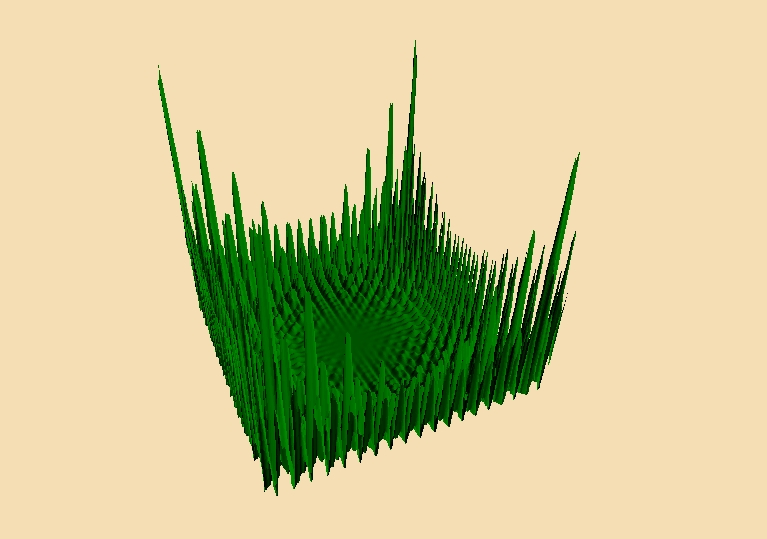
\includegraphics[scale=0.6]{/Users/guoyixuan/Documents/NTPU_STAT/images/Rplot64.jpeg}
    \caption{範例圖}
    \label{fig:scale}
  \end{figure}
\end{lstlisting}

\begin{figure}[H]
    \centering
        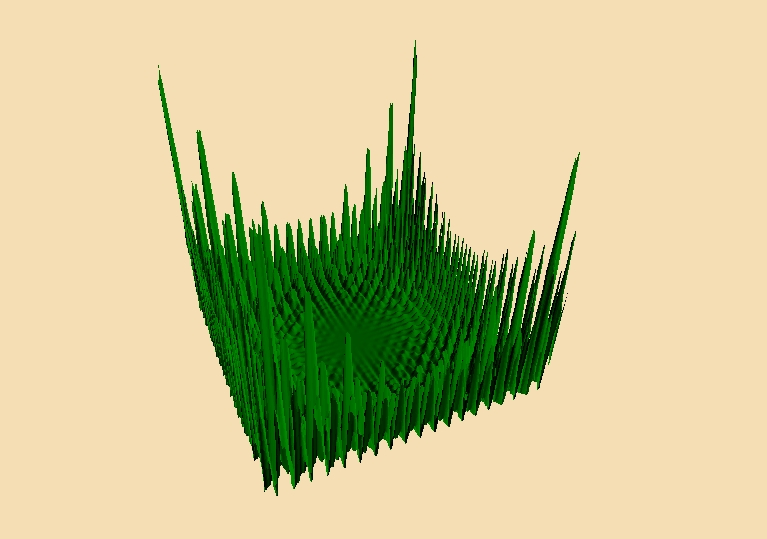
\includegraphics[scale=0.6]{/Users/guoyixuan/Documents/NTPU_STAT/images/Rplot64.jpeg}
    \caption{範例圖 (jpeg圖)}
    \label{fig:scale}
\end{figure}

圖形的大小可以透過一些指令來進行變化,我們可以利用 scale 來使原圖縮小,或者利用 width 將原圖縮小成內文行寬的 a 倍,其調整依等比例進行縮放。在圖 \ref{fig:scale} 中,本文件已經示範了在 \LaTeX 中插入 JPEG 圖,接著我們示範如何在文件中插入 EPS 檔案與 PNG 檔案,並使兩個檔案並排顯示。其中我們利用 {\A $\backslash$imgdir} 定義一個與編譯文章路徑相同的子目錄,如圖 \ref{fig:parallel}。

\textbf{圖片並排}

\bigskip
\begin{lstlisting}
   \begin{figure}[H]
    \centering
        \subfloat[範例圖 (eps圖)]{
        \includegraphics[scale=0.35]{\imgdir Rplot65.eps}}
        \subfloat[範例圖 (png圖)]{
        \includegraphics[scale=0.5]{\imgdir AnyConv.com__Rplot68.png}}
    \caption{圖形並排的作法}
    \label{fig:parallel}
  \end{figure}
\end{lstlisting}

\begin{figure}[H]
    \centering
        \subfloat[範例圖 (eps圖)]{
        \includegraphics[scale=0.35]{\imgdir Rplot65.eps}}
        \subfloat[範例圖 (png圖)]{
        \includegraphics[scale=0.5]{\imgdir AnyConv.com__Rplot68.png}}
    \caption{圖形並排的作法}
    \label{fig:parallel}
\end{figure}

\textbf{文字與圖片並排}\\
跟表格一樣,在 \LaTeX 中同樣可以使用 {\A $\backslash$minipage} 使文字與圖片並排呈現。

\begin{minipage}{.4\linewidth}
{\A minipage} 是另一種控制圖形位置的方式,適合必須與文字密切貼近的圖形。讓文字描述圖形時,可以用左圖或右圖,而不是依賴圖形編號。譬如,右圖示範的圖檔格為 PDF。此時,因為不能用 \verb|\begin{figure}|,沒有{\A label} 與  {\A caption}。

\end{minipage}
\begin{minipage}{.6\linewidth}
    \includegraphics[scale=0.6]{\imgdir Rplot62.jpeg}
\end{minipage}

\textbf{圖片旋轉}

\bigskip
\begin{lstlisting}
  \begin{figure}[H]
    \centering
        \includegraphics[angle=30,width=15cm, height=10cm]{\imgdir Rplot56.jpeg}
    \caption{旋轉圖片}
    \label{fig:angle}
  \end{figure}
\end{lstlisting}

\begin{figure}[H]
    \centering
        \includegraphics[angle=30,width=15cm, height=10cm]{\imgdir Rplot56.jpeg}
    \caption{旋轉圖片}
    \label{fig:angle}
\end{figure}

\end{document}







\documentclass[12pt, a4paper]{article} 
\usepackage{fontspec} % Font selection for XeLaTeX; see fontspec.pdf. 

\usepackage{xeCJK}	% 中文使用 XeCJK,利用 \setCJKmainfont 定義中文內文、粗體與斜體的字型
%\usepackage[BoldFont, SlantFont]{xeCJK}
% 中文使用 XeCJK,並模擬粗體與斜體(\textbf{ } \textit{ })

\defaultfontfeatures{Mapping=tex-text} 
% to support TeX conventions like ``---''
\usepackage{xunicode} 
% Unicode support for LaTeX character names(accents, European chars, etc)
\usepackage{xltxtra} 				
% Extra customizations for XeLaTeX
\usepackage{amsmath, amssymb}
\usepackage{enumerate}
\usepackage{graphicx, subfig, float, wrapfig} 
% support the \includegraphics command and options
\usepackage[outercaption]{sidecap} 
%[options]=[outercaption], [innercaption], [leftcaption], [rightcaption]
\usepackage{array, booktabs}
\usepackage{color, xcolor}
% 跨頁的超長表格;lscape是旋轉此類表格的
\usepackage{longtable, lscape}              
% 巨集,使表格加註解更容易(手冊p169)
\usepackage{threeparttable}      
% 讓表格編起來更美的套件(手冊p166),編輯跨列標題重覆的表格(手冊p182)           
\usepackage{multirow, booktabs}             
\usepackage{colortbl}     
% 直接將 latex 碼轉換成顯示文字   
\usepackage{listings}						
% 新段落前加一空行,不使用縮排

\usepackage[parfill]{parskip} 				
% 新段落前加一空行,不使用縮排

\usepackage{geometry} 
% See geometry.pdf to learn the layout options. There are lots.
%\usepackage[left=3in,right=3in,top=2in,bottom=2in]{geometry} 

\usepackage{url}

%.....表格標題註解之巨集套件.....%
% for Reference
\usepackage{natbib}			
% for Indexing				
\usepackage{makeidx}		
% Activate to begin paragraphs with an empty line rather than an indent

%章節設定
\usepackage{titlesec, titletoc,CJKnumb}		


%-----------------------------------------------------------------
%  中英文內文字型設定
%\setCJKmainfont							% 設定中文內文字型
%	[
		%BoldFont=Microsoft YaHei	    %定義粗體的字型(Win)
%		BoldFont=蘋果儷中黑	    		%定義粗體的字型(Mac)
%	]
%	{新細明體}						% 設定中文內文字型(Win)
%	{宋體-繁}							% 設定中文內文字型(Mac)	
%\setmainfont{Times New Roman}		% 設定英文內文字型
%\setsansfont{Arial}					% 無襯字字型 used with {\sffamily ...}
%\setsansfont[Scale=MatchLowercase,Mapping=tex-text]{Gill Sans}
%\setmonofont{Courier New}			% 等寬字型 used with {\ttfamily ...}
%\setmonofont[Scale=MatchLowercase]{Andale Mono}


% 英文字型
%\newfontfamily{\E}{Calibri}				
%\newfontfamily{\A}{Arial}
%\newfontfamily{\C}[Scale=0.9]{Arial}
%\newfontfamily{\R}{Times New Roman}
%\newfontfamily{\TT}[Scale=0.8]{Times New Roman}

% 中文字型
%\newCJKfontfamily{\MB}{微軟正黑體}				% 等寬及無襯線字體 Win
%\newCJKfontfamily{\SM}[Scale=0.8]{新細明體}	% 縮小版(Win)
%\newCJKfontfamily{\K}{標楷體}                	% Windows下的標楷體
%\newCJKfontfamily{\BB}{Microsoft YaHei}		% 粗體 Win
%\newCJKfontfamily{\CF}{cwTeX Q Fangsong Medium}	% CwTex 仿宋體
%\newCJKfontfamily{\CB}{cwTeX Q Hei Bold}			% CwTex 粗黑體
%\newCJKfontfamily{\CK}{cwTeX Q Kai Medium}   	% CwTex 楷體
%\newCJKfontfamily{\CM}{cwTeX Q Ming Medium}		% CwTex 明體
%\newCJKfontfamily{\CR}{cwTeX Q Yuan Medium}		% CwTex 圓體
%----------------------------------------------------------
%  中英文內文字型設定
\setCJKmainfont							% 設定中文內文字型
	[
%		BoldFont=Microsoft YaHei	    % 定義粗體的字型(Win)
		BoldFont=黑體-繁	    		    % 定義粗體的字型(Mac)
	]
%	{新細明體}						    % 設定中文內文字型(Win)
	{宋體-繁}							% 設定中文內文字型(Mac)	
\setmainfont{Times New Roman}		    % 設定英文內文字型
\setsansfont{Arial}					    % 無襯字字型 used with {\sffamily ...}
%\setsansfont[Scale=MatchLowercase,Mapping=tex-text]{Gill Sans}
\setmonofont{Courier New}			    % 等寬字型 used with {\ttfamily ...}
%\setmonofont[Scale=MatchLowercase]{Andale Mono}
% 其他字型(隨使用的電腦安裝的字型不同,用註解的方式調整(打開或關閉))
% 英文字型
\newfontfamily{\A}{Arial}
\newfontfamily{\C}{Cochin}				
\newfontfamily{\SA}[Scale=0.9]{Arial}
\newfontfamily{\R}{Times New Roman}
\newfontfamily{\ST}[Scale=0.8]{Times New Roman}
% 中文字型
%\newCJKfontfamily{\MB}{微軟正黑體}				    % 等寬及無襯線字體 Win
\newCJKfontfamily{\MB}{黑體-繁}				        % 等寬及無襯線字體 Mac
%\newCJKfontfamily{\SM}[Scale=0.8]{新細明體}	        % 縮小版(Win)
\newCJKfontfamily{\SM}[Scale=0.8]{宋體-繁}	        % 縮小版(Mac)
%\newCJKfontfamily{\K}{標楷體}                	    % Windows下的標楷體
\newCJKfontfamily{\K}{黑體-繁}               	    % Mac下的標楷體
%\newCJKfontfamily{\BB}{Microsoft YaHei}		    % 粗體 Win
\newCJKfontfamily{\BB}{宋體-繁}		                % 粗體 Mac
% 以下為自行安裝的字型:CwTex 組合
%\newCJKfontfamily{\CF}{cwTeX Q Fangsong Medium}	% CwTex 仿宋體
%\newCJKfontfamily{\CB}{cwTeX Q Hei Bold}			% CwTex 粗黑體
%\newCJKfontfamily{\CK}{cwTeX Q Kai Medium}   	    % CwTex 楷體
%\newCJKfontfamily{\CM}{cwTeX Q Ming Medium}		% CwTex 明體
%\newCJKfontfamily{\CR}{cwTeX Q Yuan Medium}		% CwTex 圓體
%-------------------------------------------------------------
\XeTeXlinebreaklocale "zh"             		
%這兩行一定要加,中文才能自動換行
\XeTeXlinebreakskip = 0pt plus 1pt     		
%這兩行一定要加,中文才能自動換行
%-----------------------------------------------------------------------------------------------------------------------


\newcommand{\cw}{\texttt{cw}\kern-.6pt\TeX}	% 這是 cwTex 的 logo 文字
\newcommand{\imgdir}{/Users/guoyixuan/Documents/NTPU_STAT/images/}				% 設定圖檔的目錄位置
\renewcommand{\tablename}{表}					% 改變表格標號文字為中文的「表」(預設為 Table)
\renewcommand{\figurename}{圖}				% 改變圖片標號文字為中文的「圖」(預設為 Figure)
\usepackage{booktabs}


% 設定顏色 see color Table: http://latexcolor.com
\usepackage{color}
\definecolor{slight}{gray}{0.9}				
\definecolor{airforceblue}{rgb}{0.36, 0.54, 0.66} 
\definecolor{arylideyellow}{rgb}{0.91, 0.84, 0.42}
\definecolor{babyblue}{rgb}{0.54, 0.81, 0.94}
\definecolor{cadmiumred}{rgb}{0.89, 0.0, 0.13}
\definecolor{coolblack}{rgb}{0.0, 0.18, 0.39}
\definecolor{beaublue}{rgb}{0.74, 0.83, 0.9}
\definecolor{beige}{rgb}{0.96, 0.96, 0.86}
\definecolor{bisque}{rgb}{1.0, 0.89, 0.77}
\definecolor{gray(x11gray)}{rgb}{0.75, 0.75, 0.75}
\definecolor{limegreen}{rgb}{0.2, 0.8, 0.2}
\definecolor{splashedwhite}{rgb}{1.0, 0.99, 1.0}

%---------------------------------------------------------------------
% 映出程式碼 \begin{lstlisting} 的內部設定
\lstset
{	language=[LaTeX]TeX,
    breaklines=true,
    %basicstyle=\tt\scriptsize,
    basicstyle=\tt\normalsize,
    keywordstyle=\color{blue},
    identifierstyle=\color{black},
    commentstyle=\color{limegreen}\itshape,
    stringstyle=\rmfamily,
    showstringspaces=false,
    %backgroundcolor=\color{splashedwhite},
    backgroundcolor=\color{slight},
    frame=single,							%default frame=none 
    rulecolor=\color{gray(x11gray)},
    framerule=0.4pt,							%expand outward 
    framesep=3pt,							%expand outward
    xleftmargin=3.4pt,		%to make the frame fits in the text area. 
    xrightmargin=3.4pt,		%to make the frame fits in the text area. 
    tabsize=2				%default :8 only influence the lstlisting and lstinline.
}

% 映出程式碼 \begin{lstlisting} 的內部設定 for Python codes
%\lstset{language=Python}
%\lstset{frame=lines}
%\lstset{basicstyle=\SCP\normalsize}
%\lstset{keywordstyle=\color{blue}}
%\lstset{commentstyle=\color{airforceblue}\itshape}
%\lstset{backgroundcolor=\color{beige}}

%%%數學式定義定理範例設定%%%
%%theroemstyle 需要使用的套件%%
\usepackage{amsthm}						
\theoremstyle{plain}

%%Definition獨立編號%%
\newtheorem{de}{定義}[section]
%%Theorem獨立編號%%
\newtheorem{thm}{{\MB 定理}}[section]		
%%lemma和theorem共同編號%%
\newtheorem{lemma}[thm]{Lemma}	
%%Example獨立編號%%
\newtheorem{ex}{{\A Example}}			

\newtheorem{cor}{Corollary}[section]		%not used here
\newtheorem{exercise}{EXERCISE}			%not used here
\newtheorem{re}{\emph{Result}}[section]	%not used here
\newtheorem{axiom}{AXIOM}				%not used here
\renewcommand{\proofname}{證明}			%not used here
\newcounter{quiz}						% start a simple and new counter
\setcounter{quiz}{1}						% start to count from 1
   % 使用自己維護的定義檔
%變更章節數字為中文數字
\geometry{a4paper,left=2.5cm,right=2.5cm,top=2cm,bottom=2cm}
\usepackage{fancyhdr}
\pagestyle{fancy}
%\fancyhf{}
%\fancyhead[LE,RO]{overleaf}
%\fancyhead[RE,LO]{guides}
%\fancyhead[CE,CO]{\leftmark}
%\fancyhead[LE,RO]{\thepage}


\title{{\MB Python 基本機率函數繪圖}}	% 使用設定的字型
\author{{\BB 郭翊萱 711133115}}				% 使用設定的小字體
\date{{\ST 2022.10. }} 			
 
\begin{document}
\maketitle
\fontsize{12}{22pt}\selectfont 
%\chapter{ {\MB Python 基本機率函數繪圖}}

Python 跟 R 是很常拿來作統計分析的程式語言,在 R 中常常使用 ggplot2 與 shiny 來繪製統計相關圖形,而在 Python 中則廣為使用 Matplotlib、Plotly 與 seaborn 來進行繪圖。在此文中,使用 Matplotlib 來進行一些基本機率函數圖形繪製,以幫助熟練使用套件 Matplotlib。另外,本文亦將在最後進行一個小專題練習。

\section{基本機率函數繪圖}
首先,本文在此介紹幾個基本機率函數圖形的繪製,以供之後利用套件 Matplotlib 進行繪圖之用。

\begin{itemize}
\item[$\bullet$] $f(x)=sin(x)+cos(x)$
\bigskip
	\begin{lstlisting}
import numpy as np
import matplotlib.pyplot as plt

x = np.linspace(-3*np.pi, 3*np.pi, 300)
y = np.sin(x) + np.cos(x)

fig, ax = plt.subplots(1)#畫布上一個圖形
ax.plot(x, y, color='skyblue')
ax.set_xticks(np.array([-3, -2, -1, 0, 1, 2, 3])*np.pi)
ax.set_xticklabels(['-3$\pi$', '-2$\pi$', '$\pi$', '0', '$\pi$','2$\pi$','3$\pi$'], \
        fontsize=10, color = 'b')
ax.set_ylim([-2, 2])
ax.grid(True)
plt.title("f(x)=sin(x)+cos(x)")
plt.show()
	\end{lstlisting}
\bigskip

\begin{figure}[H]
    \centering
        \includegraphics[scale=0.6]{/Users/guoyixuan/Documents/vscodepython/Statistical Calculation/Homework2_Function/image_hw2/1.png}
    \caption{f(x)=sin(x)+cos(x)}
    \label{fig:sincos}
\end{figure}


\item[$\bullet$] $f(x)=(1-exp(-2x))/(1+exp(-2x))$

\bigskip
\begin{lstlisting}
import matplotlib.pyplot as plt
import numpy as np
 
x = np.arange(-10,11,1)#type(x):array
# formulate a function f
f = lambda x : (1 - np.exp(-2*x)) / (1 + np.exp(-2*x))
 
fig = plt.figure(figsize=[6, 4])
plt.plot(x, f(x),  color = 'r')
plt.grid(visible = True, color='g',  linewidth=0.5)
plt.xlabel('X'), plt.ylabel('Y')
plt.ylim(-1.5,1.5)
plt.xlim(-10,10)
plt.axhline(1.01,color="b",linestyle="--")
plt.axhline(-1.01,color="b",linestyle="--")
plt.title('$f(x)=(1-exp(-2x))/(1+exp(-2x))$')
plt.show()
\end{lstlisting}

\begin{figure}[H]
    \centering
        \includegraphics[scale=0.6]{/Users/guoyixuan/Documents/vscodepython/Statistical Calculation/Homework2_Function/image_hw2/2.png}
    \caption{f(x)=(1-exp(-2x))/(1+exp(-2x))}
    \label{fig:exp}
\end{figure}

\item[$\bullet$] $f(x)=\sqrt[3]{(4-x^3)/(1+x^2)}$
\bigskip
\begin{lstlisting}
import matplotlib.pyplot as plt
import numpy as np
 
x = np.arange(-10,100,1)#type(x):array
# formulate a function f
f = lambda x : ((4-x**3)/(1+x**2))**(1/3)
 
fig = plt.figure(figsize=[6, 4])
plt.plot(x, f(x),  color = 'skyblue',linewidth=3)
plt.grid(visible = True, color='black',  linewidth=0.3)
plt.xlabel('X'), plt.ylabel('Y')
plt.title('$f(x)=f(x)=\sqrt[3]{(4-x^3)/(1+x^2)}$')
plt.show()
\end{lstlisting}

\begin{figure}[H]
    \centering
        \includegraphics[scale=0.6]{/Users/guoyixuan/Documents/vscodepython/Statistical Calculation/Homework2_Function/image_hw2/3.png}
    \caption{$f(x)=\sqrt[3]{(4-x^3)/(1+x^2)}$}
    \label{fig:exp/exp}
\end{figure}

\item[$\bullet$] $f(x)=1/x$
\bigskip
\begin{lstlisting}
import matplotlib.pyplot as plt
import numpy as np
 
x = np.arange(-50,50,1)#type(x):array
# formulate a function f
f = lambda x : 1/x
 
fig = plt.figure(figsize=[6, 4])
plt.plot(x, f(x),  color = 'green',linewidth=2)
plt.grid(visible = True, color='black',  linewidth=0.3)
plt.xlabel('X'), plt.ylabel('Y')
plt.title('$f(x)=1/x$')
plt.axhline(0,linestyle="--")
plt.axvline(0,linestyle="--")
plt.show()
\end{lstlisting}

\begin{figure}[H]
    \centering
        \includegraphics[scale=0.7]{/Users/guoyixuan/Documents/vscodepython/Statistical Calculation/Homework2_Function/image_hw2/4.png}
    \caption{$f(x)=1/x$}
    \label{fig:1/x}
\end{figure}

\item[$\bullet$] $f(x)=1/(2\sqrt{2 \pi}) \exp(-(x-1)^2/8)$
\bigskip
\begin{lstlisting}
import matplotlib.pyplot as plt
import numpy as np
 
x = np.arange(-20,20,1)#type(x):array
# formulate a function f
f = lambda x : 1/(2*np.sqrt(2*np.pi))*np.exp(-(x-1)**2/8)
 
fig = plt.figure(figsize=[6, 4])
plt.plot(x, f(x),  color = 'red',linewidth=2)
plt.grid(visible = True, color='black',  linewidth=0.3)
plt.xlabel('X'), plt.ylabel('Y')
plt.title('$f(x)=1/(2*sqrt(2*pi))exp(-(x-1)^2/8)$')
plt.show()
\end{lstlisting}

\begin{figure}[H]
    \centering
        \includegraphics[scale=0.7]{/Users/guoyixuan/Documents/vscodepython/Statistical Calculation/Homework2_Function/image_hw2/5.png}
    \caption{$f(x)=1/(2\sqrt{2 \pi}) \exp(-(x-1)^2/8)$}
    \label{fig:1/sqrt}
\end{figure}

\item[$\bullet$] $f(x)=x^{2/3}$
\bigskip
\begin{lstlisting}
import matplotlib.pyplot as plt
import numpy as np
 
x = np.arange(0,50,1)#type(x):array
# formulate a function f
f = lambda x : x**(2/3)
 
fig = plt.figure(figsize=[6, 4])
plt.plot(x, f(x),  color = 'red',linewidth=2)
plt.grid(visible = True, color='black',  linewidth=0.3)
plt.xlabel('X'), plt.ylabel('Y')
plt.title('$f(x)=x**(2/3)$')
plt.show()
\end{lstlisting}

\begin{figure}[H]
    \centering
        \includegraphics[scale=0.7]{/Users/guoyixuan/Documents/vscodepython/Statistical Calculation/Homework2_Function/image_hw2/6.png}
    \caption{$f(x)=x^{2/3}$}
    \label{fig:x^(2/3)}
\end{figure}

\item[$\bullet$]$f(x)=2x^3-x^4$
\bigskip
\begin{lstlisting}
import matplotlib.pyplot as plt
import numpy as np
 
x = np.arange(-35,35,1)#type(x):array
# formulate a function f
f = lambda x : 2*x**3-x**4
 
fig = plt.figure(figsize=[6, 4])
plt.plot(x, f(x),  color = 'red',linewidth=2)
plt.grid(visible = True, color='black',  linewidth=0.3)
plt.xlabel('X'), plt.ylabel('Y')
plt.xlim(-40,40)
plt.title('$f(x)=2*x^3-x^4$')
plt.show()
\end{lstlisting}

\begin{figure}[H]
    \centering
        \includegraphics[scale=0.7]{/Users/guoyixuan/Documents/vscodepython/Statistical Calculation/Homework2_Function/image_hw2/7.png}
    \caption{$f(x)=2x^3-x^4$}
    \label{fig:f(x)=2x^3-x^4}
\end{figure}

\item[$\bullet$]$f(x)=ln(x)/x^3$
\bigskip
\begin{lstlisting}
import matplotlib.pyplot as plt
import numpy as np
 
x = np.arange(-35,35,1)#type(x):array
# formulate a function f
f = lambda x : np.log(x)/x**3
 
fig = plt.figure(figsize=[6, 4])
plt.plot(x, f(x),  color = 'blue',linewidth=2)
plt.grid(visible = True, color='black',  linewidth=0.3)
plt.xlabel('X'), plt.ylabel('Y')
plt.xlim(0,20)
plt.title('$f(x)=ln(x)/x**3$')
plt.show()
\end{lstlisting}

\begin{figure}[H]
    \centering
        \includegraphics[scale=0.7]{/Users/guoyixuan/Documents/vscodepython/Statistical Calculation/Homework2_Function/image_hw2/8.png}
    \caption{$f(x)=ln(x)/x^3$}
    \label{fig:f(x)=ln(x)/x^3}
\end{figure}

\item[$\bullet$] $f(x)=3$, $1 \leq x \leq 5$
\bigskip
\begin{lstlisting}
import matplotlib.pyplot as plt
import numpy as np
x=[1,5]
y=[3,3]
fig, ax = plt.subplots()
ax.hlines(y=3,xmin=1,xmax=5,linewidth=2)
plt.plot(x,y,marker="o")
plt.grid(visible = True, color='black',  linewidth=0.3)
plt.xlabel('X'), plt.ylabel('Y')
plt.xlim(0,6)
plt.ylim(0,6)
plt.title('$f(x)=3$')
plt.show()
\end{lstlisting}

\begin{figure}[H]
    \centering
        \includegraphics[scale=0.6]{/Users/guoyixuan/Documents/vscodepython/Statistical Calculation/Homework2_Function/image_hw2/9.png}
    \caption{$f(x)=3$}
    \label{fig:f(x)=3}
\end{figure}

\item[$\bullet$] $x^2+y^2=1$
\bigskip
\begin{lstlisting}
import numpy as np
import matplotlib.pyplot as plt

t = np.linspace(0, 2*np.pi, 200)
r = 1
x = r*np.cos(t)
y = r*np.sin(t)

#刪掉邊線
ax=plt.gca()
ax.spines["right"].set_color("none")
ax.spines["top"].set_color("none")
#挪動x,y軸的位置
ax.spines["bottom"].set_position(("data",0))#data:將x軸綁定在y=0的位置
ax.spines["left"].set_position(("axes",0.5))#axes:將y軸綁定在x軸50%的位置
ax.set_aspect("equal")
plt.plot(x,y)
plt.xlim(-1.5,1.5)
plt.ylim(-1.5,1.5)
plt.title("Parametric Equation Circle")
plt.show()
\end{lstlisting}

\begin{figure}[H]
    \centering
        \includegraphics[scale=0.7]{/Users/guoyixuan/Documents/vscodepython/Statistical Calculation/Homework2_Function/image_hw2/10.png}
    \caption{$f(x)=3$}
    \label{fig:circle}
\end{figure}

\item[$\bullet$] Square
\bigskip
\begin{lstlisting}
import numpy as np
import matplotlib.pyplot as plt

fig, ax = plt.subplots()
ax = plt.gca()
ax.hlines(y=0.5, xmin=-0.5, xmax=0.5, linewidth=2)
ax.hlines(y=-0.5, xmin=-0.5, xmax=0.5, linewidth=2)
ax.vlines(x=0.5, ymin=-0.5, ymax=0.5, linewidth=2)
ax.vlines(x=-0.5, ymin=-0.5, ymax=0.5, linewidth=2)

ax.spines["right"].set_color("none")
ax.spines["top"].set_color("none")
ax.spines["bottom"].set_position(("data",0))#data:將x軸綁定在y=0的位置
ax.spines["left"].set_position(("axes",0.5))#axes:將y軸綁定在x軸50%的位置
ax.set_aspect("equal")

plt.xlim(-1,1)
plt.ylim(-1,1)
plt.xticks(np.arange(-1,1.5,0.5))
plt.yticks(np.arange(-1,1.5,0.5))
plt.title('A square of side 1')
plt.show()
\end{lstlisting}

\begin{figure}[H]
    \centering
        \includegraphics[scale=0.9]{/Users/guoyixuan/Documents/vscodepython/Statistical Calculation/Homework2_Function/image_hw2/11.png}
    \caption{$Square$}
    \label{fig:square}
\end{figure}

除了圖\ref{fig:square},亦可用其他方式來表達此圖,如下圖\ref{fig:square1}。
\begin{figure}[H]
    \centering
        \includegraphics[scale=0.7]{/Users/guoyixuan/Documents/vscodepython/Statistical Calculation/Homework2_Function/image_hw2/12.png}
    \caption{$Square$}
    \label{fig:square1}
\end{figure}

\end{itemize}


\section{專題練習}
接著本文列舉三個小專題來展示套件的應用。
Let $S_n=\sum_{k=1}^{n}\frac{1}{k}=1+\frac{1}{2}+\frac{1}{3+...+\frac{1}{n}}$
\begin{itemize}
\item[(a)] Verify that $\lim_{n \to \infty}S_n$ diverges.
\item[(b)] Let $\gamma_n$ denote the sum of the shade areas. Show that $\gamma_n-ln(n+1)$.
\item[(c)] Verify that $\frac{1}{2}(1-\frac{1}{n+1}) < \gamma_n < 1.$
\end{itemize}

{\bf Answer}:

\begin{itemize}
\item[(a)]
\bigskip
\begin{lstlisting}
n = 10
a = np.arange(1,n+1)
print(a)
Sn=(1/a).sum()
print(Sn)

n = 10**np.arange(3)
print(np.arange(3))#[0 1 2]
Sn=np.zeros(len(n)) #挖空集合放不同的n得到的結果
print(n)#[1 10 100]
print(np.arange(len(n)))#[0 1 2]
print(np.arange(1,n[1]+1))#[1 2 3 4 5 6 7 8 9 10]

n = 10**np.arange(10)
Sn=np.zeros(len(n)) #挖空集合放不同的n得到的結果
for i in np.arange(len(n)):
    a = np.arange(1,n[i]+1)
    Sn[i] = (1/a).sum()
print(Sn)
print(n)

x = n
y = Sn
values = [0, 1, 2, 3, 4, 5, 6, 7, 8, 9]
plt.plot(n,y)
plt.grid(visible = True, color='black',  linewidth=0.3)
plt.xlabel('n'), plt.ylabel('Sn')
plt.title('Sn diverge when n is infty')
#plt.xticks(n,values)
plt.show()
#a = np.arange(1,n[2]+1)
#print(a)
#Sn[2] = (1/a).sum()
#print(Sn[2])
\end{lstlisting}

根據以上程式碼我們可以得到下圖 \ref{fig:infty},故可得證。
\begin{figure}[H]
    \centering
        \includegraphics[scale=0.6]{/Users/guoyixuan/Documents/vscodepython/Statistical Calculation/Homework2_Function/image_hw2/13.png}
    \caption{$S_n$ diverge when $n \to \infty$}
    \label{fig:infty}
\end{figure}

\item[(b)]
\bigskip
\begin{lstlisting}
import numpy as np
import matplotlib.pyplot as plt

x = np.arange(0,1000,0.1)#type(x):array
# formulate a function f
f = lambda x : 1/x
 
fig = plt.figure(figsize=[6, 4])
plt.plot(x, f(x),  color = 'blue',linewidth=2)
plt.grid(visible = True, color='black',  linewidth=0.3)
plt.xlabel('X'), plt.ylabel('Y')
plt.xlim(0,10)
plt.ylim(0,2)
plt.xticks(np.arange(0,11,1))
plt.title('$f(x)=1/x$')
plt.show()

def func(x):
    return 1/x
x = np.linspace(2,3,1000)
dx = (3-2)/1000
y = func(x)
area = np.sum(y*dx)
#print(func(2)-area)
#print(1-np.log(2))

n = np.arange(1,101)#[1 2 3 4 5 6 7 8 9 10]
gamma2=np.zeros(len(n))
def func(x):
    return 1/x
for i in np.arange(len(n)):#[0 1 2 3 4 5 6 7 8 9]
    x = np.linspace(n[i],n[i]+1,1000)
    dx = (2-1)/1000
    y = func(x)
    area = np.sum(y*dx)
    gamma2[i] = func(i+1)-area+gamma2[i-1]
print(gamma2)

n = np.arange(1,101)#[1 2 3 4 5 6 7 8 9 10]
Sn = np.zeros(len(n))
gamma1 = np.zeros(len(n))
for i in np.arange(len(n)):#[0 1 2 3 4 5 6 7 8 9]
    a = np.arange(1,n[i]+1)
    Sn[i] = (1/a).sum()
    gamma1[i] = Sn[i]-np.log(n[i]+1)
#print(Sn)
print(gamma1)
print(3/2-np.log(3))

fig, ax = plt.subplots(figsize = (9,6))
plt.subplot(1,2,1)
plt.plot(n,gamma1,color="red")
plt.grid(visible = True, color='black',  linewidth=0.3)
plt.xlabel('n'), plt.ylabel('gamma_n')
plt.title('gamma_n ')

plt.subplot(1,2,2)
plt.plot(n,gamma2,color="blue")
plt.grid(visible = True, color='black',  linewidth=0.3)
plt.xlabel('n'), plt.ylabel('Sn+ln(n+1)')
plt.title('Sn+ln(n+1)')
plt.show()

\end{lstlisting}

\begin{figure}[H]
    \centering
        \includegraphics[scale=0.6]{/Users/guoyixuan/Documents/vscodepython/Statistical Calculation/Homework2_Function/image_hw2/15.png}
    \caption{$\gamma_n$ and $S_n+ln(n+1)$}
    \label{fig:gamma_n}
\end{figure}

根據圖 \ref{fig:gamma_n} 以及以上程式碼我們可以求得從 $n=1$ 到 $n=100$ 時,$\gamma_n$ 與 $S_n+ln(n+1)$ 個別的值,由此可以發現兩者的值基本趨近相同,故可得證。

另外,我們也可直接利用數學進行證明,其過程如下:
$$\gamma_n=\sum_{k=1}^{n} \int_{x=k}^{k+1}(\frac{1}{k}-\frac{1}{x})dx 
=\sum_{k=1}^{n}(\int_{k}^{k+1}\frac{1}{k}-\int_{k}^{k+1}\frac{1}{x} dx)=\sum_{k=1}^{n}(\frac{1}{k}-ln \left| k+1 \right|+ln \left| k \right|)$$
$$=S_n-(ln2+ln3+...+ln(n)+ln(n+1))+(ln1+ln2+ln3+...+ln(n))$$
$$=S_n-ln(n+1)$$

\item[(c)]
\bigskip
\begin{lstlisting}
import numpy as np
import matplotlib.pyplot as plt

x = np.arange(0,1000,0.1)#type(x):array
# formulate a function f
f = lambda x : 1/x

n = np.arange(1,101)#[1 2 3 4 5 6 7 8 9 10]
gamma2=np.zeros(len(n))
def func(x):
    return 1/x
for i in np.arange(len(n)):#[0 1 2 3 4 5 6 7 8 9]
    x = np.linspace(n[i],n[i]+1,1000)
    dx = (2-1)/1000
    y = func(x)
    area = np.sum(y*dx)
    gamma2[i] = func(i+1)-area+gamma2[i-1]

n = np.arange(1,101)
theta = np.zeros(len(n))
for i in np.arange(len(n)):
    theta[i] = 1/2*(1-1/(n[i]+1))


fig, ax = plt.subplots(figsize = (9,6))
plt.plot(n,gamma2,label="gamma_n",color="green")
plt.plot(n,theta,label="1/2(1-1/(n+1))",color="blue")
plt.axhline(1,color="red",label="1")
plt.ylim(0,1.1)
plt.xlim(0,100)
plt.xticks(np.arange(0,100,20))
plt.yticks(np.arange(0,1.1,0.1))
plt.grid(visible = True, color='black',  linewidth=0.3)
plt.xlabel('n'), plt.ylabel('Sn+ln(n+1)')

plt.legend(loc="lower right")
plt.show()

\end{lstlisting}

由上面程式碼與圖 \ref{fig:gamma_n2} 我們即可得證$\frac{1}{2}(1-\frac{1}{n+1}) < \gamma_n < 1$。

\begin{figure}[H]
    \centering
        \includegraphics[scale=0.6]{/Users/guoyixuan/Documents/vscodepython/Statistical Calculation/Homework2_Function/image_hw2/16.png}
    \caption{$\frac{1}{2}(1-\frac{1}{n+1}) < \gamma_n < 1$}
    \label{fig:gamma_n2}
\end{figure}

\end{itemize}

\section{小結}

在上面兩節,我們練習了套件 Matplotlib 的基本繪圖技巧,並也由此對機率函數有一些更深入的認知,望對以後使用 Python 進行繪圖有所幫助。


\end{document}
\documentclass[12pt, a4paper]{article} 
\usepackage{fontspec} % Font selection for XeLaTeX; see fontspec.pdf. 

\usepackage{xeCJK}	% 中文使用 XeCJK,利用 \setCJKmainfont 定義中文內文、粗體與斜體的字型
%\usepackage[BoldFont, SlantFont]{xeCJK}
% 中文使用 XeCJK,並模擬粗體與斜體(\textbf{ } \textit{ })

\defaultfontfeatures{Mapping=tex-text} 
% to support TeX conventions like ``---''
\usepackage{xunicode} 
% Unicode support for LaTeX character names(accents, European chars, etc)
\usepackage{xltxtra} 				
% Extra customizations for XeLaTeX
\usepackage{amsmath, amssymb}
\usepackage{enumerate}
\usepackage{graphicx, subfig, float, wrapfig} 
% support the \includegraphics command and options
\usepackage[outercaption]{sidecap} 
%[options]=[outercaption], [innercaption], [leftcaption], [rightcaption]
\usepackage{array, booktabs}
\usepackage{color, xcolor}
% 跨頁的超長表格;lscape是旋轉此類表格的
\usepackage{longtable, lscape}              
% 巨集,使表格加註解更容易(手冊p169)
\usepackage{threeparttable}      
% 讓表格編起來更美的套件(手冊p166),編輯跨列標題重覆的表格(手冊p182)           
\usepackage{multirow, booktabs}             
\usepackage{colortbl}     
% 直接將 latex 碼轉換成顯示文字   
\usepackage{listings}						
% 新段落前加一空行,不使用縮排

\usepackage[parfill]{parskip} 				
% 新段落前加一空行,不使用縮排

\usepackage{geometry} 
% See geometry.pdf to learn the layout options. There are lots.
%\usepackage[left=3in,right=3in,top=2in,bottom=2in]{geometry} 

\usepackage{url}

%.....表格標題註解之巨集套件.....%
% for Reference
\usepackage{natbib}			
% for Indexing				
\usepackage{makeidx}		
% Activate to begin paragraphs with an empty line rather than an indent

%章節設定
\usepackage{titlesec, titletoc,CJKnumb}		


%-----------------------------------------------------------------
%  中英文內文字型設定
%\setCJKmainfont							% 設定中文內文字型
%	[
		%BoldFont=Microsoft YaHei	    %定義粗體的字型(Win)
%		BoldFont=蘋果儷中黑	    		%定義粗體的字型(Mac)
%	]
%	{新細明體}						% 設定中文內文字型(Win)
%	{宋體-繁}							% 設定中文內文字型(Mac)	
%\setmainfont{Times New Roman}		% 設定英文內文字型
%\setsansfont{Arial}					% 無襯字字型 used with {\sffamily ...}
%\setsansfont[Scale=MatchLowercase,Mapping=tex-text]{Gill Sans}
%\setmonofont{Courier New}			% 等寬字型 used with {\ttfamily ...}
%\setmonofont[Scale=MatchLowercase]{Andale Mono}


% 英文字型
%\newfontfamily{\E}{Calibri}				
%\newfontfamily{\A}{Arial}
%\newfontfamily{\C}[Scale=0.9]{Arial}
%\newfontfamily{\R}{Times New Roman}
%\newfontfamily{\TT}[Scale=0.8]{Times New Roman}

% 中文字型
%\newCJKfontfamily{\MB}{微軟正黑體}				% 等寬及無襯線字體 Win
%\newCJKfontfamily{\SM}[Scale=0.8]{新細明體}	% 縮小版(Win)
%\newCJKfontfamily{\K}{標楷體}                	% Windows下的標楷體
%\newCJKfontfamily{\BB}{Microsoft YaHei}		% 粗體 Win
%\newCJKfontfamily{\CF}{cwTeX Q Fangsong Medium}	% CwTex 仿宋體
%\newCJKfontfamily{\CB}{cwTeX Q Hei Bold}			% CwTex 粗黑體
%\newCJKfontfamily{\CK}{cwTeX Q Kai Medium}   	% CwTex 楷體
%\newCJKfontfamily{\CM}{cwTeX Q Ming Medium}		% CwTex 明體
%\newCJKfontfamily{\CR}{cwTeX Q Yuan Medium}		% CwTex 圓體
%----------------------------------------------------------
%  中英文內文字型設定
\setCJKmainfont							% 設定中文內文字型
	[
%		BoldFont=Microsoft YaHei	    % 定義粗體的字型(Win)
		BoldFont=黑體-繁	    		    % 定義粗體的字型(Mac)
	]
%	{新細明體}						    % 設定中文內文字型(Win)
	{宋體-繁}							% 設定中文內文字型(Mac)	
\setmainfont{Times New Roman}		    % 設定英文內文字型
\setsansfont{Arial}					    % 無襯字字型 used with {\sffamily ...}
%\setsansfont[Scale=MatchLowercase,Mapping=tex-text]{Gill Sans}
\setmonofont{Courier New}			    % 等寬字型 used with {\ttfamily ...}
%\setmonofont[Scale=MatchLowercase]{Andale Mono}
% 其他字型(隨使用的電腦安裝的字型不同,用註解的方式調整(打開或關閉))
% 英文字型
\newfontfamily{\A}{Arial}
\newfontfamily{\C}{Cochin}				
\newfontfamily{\SA}[Scale=0.9]{Arial}
\newfontfamily{\R}{Times New Roman}
\newfontfamily{\ST}[Scale=0.8]{Times New Roman}
% 中文字型
%\newCJKfontfamily{\MB}{微軟正黑體}				    % 等寬及無襯線字體 Win
\newCJKfontfamily{\MB}{黑體-繁}				        % 等寬及無襯線字體 Mac
%\newCJKfontfamily{\SM}[Scale=0.8]{新細明體}	        % 縮小版(Win)
\newCJKfontfamily{\SM}[Scale=0.8]{宋體-繁}	        % 縮小版(Mac)
%\newCJKfontfamily{\K}{標楷體}                	    % Windows下的標楷體
\newCJKfontfamily{\K}{黑體-繁}               	    % Mac下的標楷體
%\newCJKfontfamily{\BB}{Microsoft YaHei}		    % 粗體 Win
\newCJKfontfamily{\BB}{宋體-繁}		                % 粗體 Mac
% 以下為自行安裝的字型:CwTex 組合
%\newCJKfontfamily{\CF}{cwTeX Q Fangsong Medium}	% CwTex 仿宋體
%\newCJKfontfamily{\CB}{cwTeX Q Hei Bold}			% CwTex 粗黑體
%\newCJKfontfamily{\CK}{cwTeX Q Kai Medium}   	    % CwTex 楷體
%\newCJKfontfamily{\CM}{cwTeX Q Ming Medium}		% CwTex 明體
%\newCJKfontfamily{\CR}{cwTeX Q Yuan Medium}		% CwTex 圓體
%-------------------------------------------------------------
\XeTeXlinebreaklocale "zh"             		
%這兩行一定要加,中文才能自動換行
\XeTeXlinebreakskip = 0pt plus 1pt     		
%這兩行一定要加,中文才能自動換行
%-----------------------------------------------------------------------------------------------------------------------


\newcommand{\cw}{\texttt{cw}\kern-.6pt\TeX}	% 這是 cwTex 的 logo 文字
\newcommand{\imgdir}{/Users/guoyixuan/Documents/NTPU_STAT/images/}				% 設定圖檔的目錄位置
\renewcommand{\tablename}{表}					% 改變表格標號文字為中文的「表」(預設為 Table)
\renewcommand{\figurename}{圖}				% 改變圖片標號文字為中文的「圖」(預設為 Figure)
\usepackage{booktabs}


% 設定顏色 see color Table: http://latexcolor.com
\usepackage{color}
\definecolor{slight}{gray}{0.9}				
\definecolor{airforceblue}{rgb}{0.36, 0.54, 0.66} 
\definecolor{arylideyellow}{rgb}{0.91, 0.84, 0.42}
\definecolor{babyblue}{rgb}{0.54, 0.81, 0.94}
\definecolor{cadmiumred}{rgb}{0.89, 0.0, 0.13}
\definecolor{coolblack}{rgb}{0.0, 0.18, 0.39}
\definecolor{beaublue}{rgb}{0.74, 0.83, 0.9}
\definecolor{beige}{rgb}{0.96, 0.96, 0.86}
\definecolor{bisque}{rgb}{1.0, 0.89, 0.77}
\definecolor{gray(x11gray)}{rgb}{0.75, 0.75, 0.75}
\definecolor{limegreen}{rgb}{0.2, 0.8, 0.2}
\definecolor{splashedwhite}{rgb}{1.0, 0.99, 1.0}

%---------------------------------------------------------------------
% 映出程式碼 \begin{lstlisting} 的內部設定
\lstset
{	language=[LaTeX]TeX,
    breaklines=true,
    %basicstyle=\tt\scriptsize,
    basicstyle=\tt\normalsize,
    keywordstyle=\color{blue},
    identifierstyle=\color{black},
    commentstyle=\color{limegreen}\itshape,
    stringstyle=\rmfamily,
    showstringspaces=false,
    %backgroundcolor=\color{splashedwhite},
    backgroundcolor=\color{slight},
    frame=single,							%default frame=none 
    rulecolor=\color{gray(x11gray)},
    framerule=0.4pt,							%expand outward 
    framesep=3pt,							%expand outward
    xleftmargin=3.4pt,		%to make the frame fits in the text area. 
    xrightmargin=3.4pt,		%to make the frame fits in the text area. 
    tabsize=2				%default :8 only influence the lstlisting and lstinline.
}

% 映出程式碼 \begin{lstlisting} 的內部設定 for Python codes
%\lstset{language=Python}
%\lstset{frame=lines}
%\lstset{basicstyle=\SCP\normalsize}
%\lstset{keywordstyle=\color{blue}}
%\lstset{commentstyle=\color{airforceblue}\itshape}
%\lstset{backgroundcolor=\color{beige}}

%%%數學式定義定理範例設定%%%
%%theroemstyle 需要使用的套件%%
\usepackage{amsthm}						
\theoremstyle{plain}

%%Definition獨立編號%%
\newtheorem{de}{定義}[section]
%%Theorem獨立編號%%
\newtheorem{thm}{{\MB 定理}}[section]		
%%lemma和theorem共同編號%%
\newtheorem{lemma}[thm]{Lemma}	
%%Example獨立編號%%
\newtheorem{ex}{{\A Example}}			

\newtheorem{cor}{Corollary}[section]		%not used here
\newtheorem{exercise}{EXERCISE}			%not used here
\newtheorem{re}{\emph{Result}}[section]	%not used here
\newtheorem{axiom}{AXIOM}				%not used here
\renewcommand{\proofname}{證明}			%not used here
\newcounter{quiz}						% start a simple and new counter
\setcounter{quiz}{1}						% start to count from 1
   % 使用自己維護的定義檔
%變更章節數字為中文數字
\geometry{a4paper,left=2.5cm,right=2.5cm,top=2cm,bottom=2cm}
\usepackage{fancyhdr}
\pagestyle{fancy}
\fancyhf{}
%\fancyhead[LE,RO]{overleaf}
%\fancyhead[RE,LO]{guides}
%\fancyhead[CE,CO]{\leftmark}
%\fancyhead[LE,RO]{\thepage}


\title{{\MB 機率分配與抽樣分配}}	% 使用設定的字型
\author{{\BB 郭翊萱 711133115}}				% 使用設定的小字體
\date{{\ST 2022.11 }} 			
 
\begin{document}
\maketitle
\fontsize{12}{22pt}\selectfont 
%\chapter{{\MB 機率分配與抽樣分配}}

統計學的基礎是機率,而我們需要更了解每個分配的基本性質才能更好的理解統計學,並做出正確的分析。因此在此文件中,我們首先將討論在改變參數時,幾種常見的離散分配與連續分配的機率密度圖與累積機率圖,接著,我們會利用抽樣分配來探討幾種分配之間的關係,並以直方圖、qqplot 圖、箱型圖與 edcf 圖進行呈現。最後,我們將以一個小專題來進行此節的收尾。

\section{Discrete Distributions}

在此節中,我們將介紹幾種常見的離散型分配,包含二項分配(Binomial Distribution)、超幾何分配(Hypergeometric Distribution)、幾何分配(Geometric Distribution)與卜瓦松分配 (Poisson Distribution)。首先我們先介紹二項分配。

\subsection{Binomial Distribution}

二項分配是 n 個獨立的試驗中成功次數的離散機率分布,每次成功的機率都設為p,而一次成功的分配則稱為伯努利分配。以下我們透過改變二項分配的參數來繪製其機率分布圖。
\begin{figure}[H]
    \centering
        \includegraphics[scale=0.5]{/Users/guoyixuan/Documents/vscodepython/Statistical Calculation/Homework3_Distribution/image_hw3/binom.eps}
    \caption{cdf and pdf of Binomial Distribution}
    \label{fig:Binomial Distribution}
\end{figure}

    以上圖 \ref{fig:Binomial Distribution} 即為二項分配的pmf圖與cdf圖。我們透過改變n (綠色 stem 圖)以及改變p (藍色 stem 圖)分別繪製二項分配的pmf 圖。先觀察綠色的  pmf 圖,我們令 n = 50, 70, 90, 110、p為0.7來繪製 pmf 圖,由圖 \ref{fig:Binomial Distribution} 可知,隨著n值變大,整個圖型會往右偏移,且會逐漸趨近於鐘型分配,似乎與常態分配趨近。接著我們觀察藍色的pmf圖,我們令 n 為100、p = 0.3, 0.6, 0.9來繪製機率圖,由圖 \ref{fig:Binomial Distribution} 同樣可以發現,隨著 p 增大,圖型也會逐漸向右移動,即期望值變大,且圖型的最高點也從0.08左右升至0.12左右。

\bigskip
\begin{lstlisting}
n = np.arange(50, 120, 20)
p = 0.7
x = np.linspace(20, 100, 50)
for i in n:
    y = binom.pmf(x, i, p)
    axes[0].stem(x, y, linefmt='g-', markerfmt='o', basefmt = 'C1--')
n = 100
p = np.arange(0.3, 0.9, 0.3)
for i in p:
    y = binom.pmf(x, n, i)
    axes[0].stem(x, y, linefmt='b:', markerfmt='o', basefmt = 'C1--')
\end{lstlisting}

以上即為繪製pmf圖所需之程式碼,其中 linefmt 可以改變 stem 圖的線條型狀以及線條顏色,markerfmt 則可以改變端點的形狀。

透過圖 \ref{fig:Binomial Distribution} 同樣可以觀察二項分配的 cdf 圖,我們繪製三組不同 (n, p) 情況下的 cdf 圖,包含 (20, 0.5), (30, 0.6) 以及 (40, 0.7),隨著 n 與 p 的值增加,cdf 圖會整體向右移動。

\textbf{Binomial Approximation}

在此我們以二項分配 B(100, 0.1) 與常態分配 N(10, 3) 舉例,由圖 \ref{fig:Binomial Approximation} 可知,二項分配在樣本數夠大且 $np > 5$ 時會趨近常態分配。

\begin{figure}[H]
    \centering
        \includegraphics[scale=0.5]{/Users/guoyixuan/Documents/vscodepython/Statistical Calculation/Homework3_Distribution/image_hw3/binom-norm.eps}
    \caption{Binomial Approximate to Normal Distribution}
    \label{fig:Binomial Approximation}
\end{figure}


\subsection{Hypergeometric Distribution}

超幾何分配 (Hypergeometric Distribution) 是統計學上的一種離散型分配,代表從有限的 M 個物件中抽取 N 個物件,並成功從其中指定的 N 個物件中抽出 x 個物件的機率(取出不放回)。

\begin{figure}[H]
    \centering
        \includegraphics[scale=0.6]{/Users/guoyixuan/Documents/vscodepython/Statistical Calculation/Homework3_Distribution/image_hw3/hyper.png}
    \caption{Binomial Approximate to Normal Distribution}
    \label{fig:Hypergeometric Distribution}
\end{figure}

我們透過改變 n 以及 N 來繪製 pmf 圖進行觀察,透過圖 \ref{fig:Hypergeometric Distribution} 可知,隨著 n 與 N 的值增加,超幾何分配的圖形也會逐漸向右偏移,即期望值變大,而且圖型的最高點會逐漸變小,從0.15左右下降至0.1左右。

\subsection{Geometric Distribution}
幾何分配 (Geometric Distribution) 可以用兩者方法來進行解釋,第一種解釋是 "在伯努利試驗中,得到一次成功所需的試驗次數(X)",另一種意思則為 "在得到第一次成功之前所經歷的失敗次數(Y=X-1)"。其 pmf 為:

\begin{equation}
P(X=k)=(1-p)^{k-1}p
\end{equation}

其中 $k = 1,2,3,...$

我們透過變更參數 p 來觀察幾何分配的 pmf 圖,透過觀察圖 \ref{fig:Geometric Distribution} 我們可知,我們設 p = 0.2, 0.4, 0.5, 0.7 來進行觀察,隨著 p 的值增大,pmf 圖的端點從0.2增至0.7,其尾部也從遞減至 $x=12$ 變成遞減至 $x=6$ 左右。

\begin{figure}[H]
    \centering
        \includegraphics[scale=0.6]{/Users/guoyixuan/Documents/vscodepython/Statistical Calculation/Homework3_Distribution/image_hw3/geom.eps}
    \caption{Geometric Distribution}
    \label{fig:Geometric Distribution}
\end{figure}


\subsection{Poisson Distribution}

卜瓦松分配 (Poisson Distribution) 是用於描述單位時間內隨機事件發生的次數的機率分配,其參數 $\lambda$ 為隨機事件發生次數的期望值,其機率質量函數則為:

\begin{equation}
P(X=k)=\frac{e^{-\lambda}\lambda^k}{k!}
\end{equation}

\begin{figure}[H]
    \centering
        \includegraphics[scale=0.6]{/Users/guoyixuan/Documents/vscodepython/Statistical Calculation/Homework3_Distribution/image_hw3/poisson.eps}
    \caption{Poisson Distribution}
    \label{fig:Poisson Distribution}
\end{figure}

我們透過改變參數 $\lambda$ 來觀察卜瓦松分配的 pmf 圖,由圖 \ref{fig:Poisson Distribution} 可知,我們設定參數 $\lambda=1, 4, 6, 8$,當 $\lambda$ 較小時,卜瓦松分配為右偏分配,而當 $\lambda$ 較大時,卜瓦松分配則為鐘型分配,可能趨近常態分配。

\textbf{Binomial Approximate to Poisson Distribution}

在數理統計課程中,我們可知當 n 趨近於無限大、p 趨近於0時二項分配會趨近於卜瓦松分配,因此在此處我們透過改變二項分配的參數 n, p 以及卜瓦松分配的參數 $\lambda$ 來觀察此趨近特性。我們設置 $\lambda=np$。

\begin{figure}[H]
    \centering
        \includegraphics[scale=0.6]{/Users/guoyixuan/Documents/vscodepython/Statistical Calculation/Homework3_Distribution/image_hw3/binom-poisson.eps}
    \caption{Binomial approximate to Poisson Distribution}
    \label{fig:Binomial approximate to Poisson Distribution}
\end{figure}

由圖 \ref{fig:Binomial approximate to Poisson Distribution} 的左上圖與右上圖可知,當 $n=20$、$p=0.05$ 時,二項分配趨近於卜瓦松分配,但當 $n=20$、$p=0.5$ 時,二項分配不會趨近於卜瓦松分配。

接著,根據圖 \ref{fig:Binomial approximate to Poisson Distribution} 的 左下圖與右下圖可知,當 n 夠大且 p 夠小時二項分配會趨近於卜瓦松分配,而當 n 夠大但 p 不夠小時,二項分配不會趨近於卜瓦松分配。下面即為部分程式碼示例。

\bigskip
\begin{lstlisting}
fig, axes = plt.subplots(2, 2, figsize=(10, 5))
x = np.linspace(1, 6, 50)

n, p = 10, 0.05
lamb = n*p
y = binom.pmf(x, n, p)
axes[1][0].stem(x, y, label="B(n={},p={})".format(n,p))
y1 = poisson.pmf(x, lamb)
axes[1][0].stem(x, y1, linefmt='g:', label="Poisson($\lambda$={})".format(lamb))
axes[1][1].set_xlabel("x")

plt.savefig(img_dir+"binom-poisson.eps", format="eps")
plt.show()
\end{lstlisting}

\textbf{Poisson Distribution Addiction}

在數理統計中,我們同樣學到當 $X \sim Poisson(\lambda_{1})$、$X \sim Poisson(\lambda_{2})$ 時,$X+Y \sim Poisson(\lambda_{1}+\lambda_{2})$,即卜瓦松分配具有加成性。因此在此處,我們將利用亂數產生 X 與 Y 的卜瓦松分配隨機變數,並與 $X+Y \sim Poisson(\lambda_{1}+\lambda_{2})$ 的 pmf圖進行比較。在此處中,我們繪製直方圖 (Histogram)、箱型圖 (Boxplot)、常態機率圖與 Empirical CDF 圖來進行觀察,並觀察如果更改亂數產生的樣本大小 (n) 是否會使結果發生改變。

\begin{figure}[H]
    \centering
        \includegraphics[scale=0.6]{/Users/guoyixuan/Documents/vscodepython/Statistical Calculation/Homework3_Distribution/image_hw3/sampling poisson n=80.eps}
    \caption{$X+Y \sim Poisson(\lambda_{1}+\lambda_{2})$, $n=80$}
    \label{fig:Poisson Addiction when n = 80}
\end{figure}

我們設定$\lambda=3$ 以及 $\lambda=4$ 來繪製圖形,圖 \ref{fig:Poisson Addiction when n = 80} 即為利用亂數產生圖形的結果。由此圖可知,雖然 qqplot 圖基本上貼合 $Poisson(\lambda_{1}+\lambda_{2})$ 的 pmf 圖,但從其直方圖與 ecdf 圖卻可以看出,似乎亂數產生的分配的 ecdf 與 $Poisson(\lambda_{1}+\lambda_{2})$ 的 cdf 圖 並未完全貼合。以下為部分繪圖程式碼。

\bigskip
\begin{lstlisting}
np.random.seed(seed=1294) #設定種子

n = 1000
lamb1 = 3
x1 = poisson.rvs(lamb1, size = n)
lamb2 = 4
x2 = poisson.rvs(lamb2, size = n)

##兩個亂數抽樣分配相加
x4 = x1+x2
bins = 10
axes[0][0].hist(x4, density=True, bins = bins, alpha=0.5, color="y")

###Poisson分配(lamb1+lamb2)
x3 = np.linspace(0, 20, 50)
lamb3 = lamb1+lamb2
y = poisson.pmf(x3, lamb3)
axes[0][0].stem(x3, y)

##ECDF##
x_sort = np.sort(x4)
F = np.arange(1 ,n+1) / n 
axes[1][1].plot(x_sort, F, lw =3, label = "Empirical CDF")

X = np.linspace(x_sort[0], x_sort[-1], 1000)
y = poisson.cdf(X, lamb3)
axes[1][1].plot(X, y, linestyle="--", lw = 3, label = "real cdf")
\end{lstlisting}

\begin{figure}[H]
    \centering
        \includegraphics[scale=0.6]{/Users/guoyixuan/Documents/vscodepython/Statistical Calculation/Homework3_Distribution/image_hw3/sampling poisson n=1000.eps}
    \caption{$X+Y \sim Poisson(\lambda_{1}+\lambda_{2})$, $n=1000$}
    \label{fig:Poisson Addiction when n = 1000}
\end{figure}

在圖 \ref{fig:Poisson Addiction when n = 1000} 中我們可以看出,與 $n=80$ 時不同的是,此時的qqplot圖完全貼合,且 ecdf 圖與真實的 $Poisson(\lambda_{1}+\lambda_{2})$ 也已完全貼近,由此可證。\\

\textbf{Sampling Poisson Distribution}

以下我們利用亂數抽取卜瓦松分配並繪製直方圖與 qqplot 圖,並觀察其與常態分配的差異以及樣本數改變可能導致的差異。在此我們以 Normal($\mu,\sigma$)作為比較,觀察 Poisson(2), Poisson(5) 與 Poisson(20) 三個分配。我們首先觀察在樣本數 n=20, n=100, n=1000 時的直方圖。

\begin{figure}[H]
    \centering
        \includegraphics[scale=0.5]{/Users/guoyixuan/Documents/vscodepython/Statistical Calculation/Homework3_Distribution/image_hw3/sampling-poinormal-hist-n=20.eps}
    \caption{Sampling Poisson Distribution, n=20}
    \label{fig:sampling-poinormal-hist-n=20}
\end{figure}

從圖 \ref{fig:sampling-poinormal-hist-n=20} 可知,在樣本數為20時,從直方圖中似乎無法觀察出甚麼特別的性質。接著,我們將樣本數增加至$n=100$,甚至是 $n=1000$,如下圖 \ref{fig:sampling-poinormal-hist-n=100} 與 \ref{fig:sampling-poinormal-hist-n=1000}。

\begin{figure}[H]
    \centering
        \includegraphics[scale=0.5]{/Users/guoyixuan/Documents/vscodepython/Statistical Calculation/Homework3_Distribution/image_hw3/sampling-poinormal-hist-n=100.eps}
    \caption{Sampling Poisson Distribution, n=100}
    \label{fig:sampling-poinormal-hist-n=100}
\end{figure}

\begin{figure}[H]
    \centering
        \includegraphics[scale=0.5]{/Users/guoyixuan/Documents/vscodepython/Statistical Calculation/Homework3_Distribution/image_hw3/sampling-poinormal-hist-n=1000.eps}
    \caption{Sampling Poisson Distribution, n=1000}
    \label{fig:sampling-poinormal-hist-n=1000}
\end{figure}

根據上圖 \ref{fig:sampling-poinormal-hist-n=100} 與 \ref{fig:sampling-poinormal-hist-n=1000} 我們可以發現,隨著樣本數變大以及卜瓦松分配的參數值變大,卜瓦松分配的直方圖會越來越趨近於鐘型分配的形狀。接著我們來觀察不同樣本數下卜瓦松分配的 qqplot 圖。

\begin{figure}[H]
    \centering
        \includegraphics[scale=0.5]{/Users/guoyixuan/Documents/vscodepython/Statistical Calculation/Homework3_Distribution/image_hw3/sampling-poinormal-qqplot-n=20.eps}
    \caption{Sampling Poisson Distribution, n=20}
    \label{fig:sampling-poinormal-qqplot-n=20}
\end{figure}

由圖 \ref{fig:sampling-poinormal-qqplot-n=20} 可觀察在樣本數為20的情況下,卜瓦松分配與常態分配的 qqplot 圖,在此圖中仍然可以觀察到卜瓦松分配的離散性質。接著,我們將樣本數增加至n = 100 甚至是 n = 1000 再重新繪製 qqplot 圖,如圖 \ref{fig:sampling-poinormal-qqplot-n=100} 與 \ref{fig:sampling-poinormal-qqplot-n=1000}。

\begin{figure}[H]
    \centering
        \includegraphics[scale=0.5]{/Users/guoyixuan/Documents/vscodepython/Statistical Calculation/Homework3_Distribution/image_hw3/sampling-poinormal-qqplot-n=100.eps}
    \caption{Sampling Poisson Distribution, n=100}
    \label{fig:sampling-poinormal-qqplot-n=100}
\end{figure}

\begin{figure}[H]
    \centering
        \includegraphics[scale=0.5]{/Users/guoyixuan/Documents/vscodepython/Statistical Calculation/Homework3_Distribution/image_hw3/sampling-poinormal-qqplot-n=1000.eps}
    \caption{Sampling Poisson Distribution, n=1000}
    \label{fig:sampling-poinormal-qqplot-n=1000}
\end{figure}

由上圖 \ref{fig:sampling-poinormal-qqplot-n=100} 與 \ref{fig:sampling-poinormal-qqplot-n=1000} 可觀察到,隨著樣本數增大,卜瓦松分配會與常態分配越來越貼近,此觀察到的結果與我們在數理統計課程中所了解到的性質一致。以下我們簡略呈現部分程式碼:

\bigskip
\begin{lstlisting}
mu = 4
sigma = 3
n = 1000
rv_norm = norm.rvs(loc = mu, scale = sigma, size = n)
lamb1 = 2
lamb2 = 5
lamb3 = 20
rv_poi1 = poisson.rvs(lamb1, size = n)
rv_poi2 = poisson.rvs(lamb2, size = n)
rv_poi3 = poisson.rvs(lamb3, size = n)
ax1.hist(rv_norm, bins = bins, density=True, color="r", alpha = 0.5)
stats.probplot(rv_poi1, dist = "norm", plot = ax2)
\end{lstlisting}


\section{Continuous Distributions}

\subsection{Chi-squared Distribution}

k 個獨立的標準常態分配變數的平方和服從自由度為 k 卡方分配,卡方分配也是一種特殊的伽瑪分配。其機率密度函數為:

\begin{equation}
f_k(x)=\frac{1}{2^{\frac{k}{2}}\Gamma{(\frac{k}{2})}}2^{\frac{k}{2}-1}e^{\frac{-x}{2}}
\end{equation}

\begin{figure}[H]
    \centering
        \includegraphics[scale=0.6]{/Users/guoyixuan/Documents/vscodepython/Statistical Calculation/Homework3_Distribution/image_hw3/chi-squared.eps}
    \caption{Chi-squared Distribution}
    \label{fig:Chi-squared Distribution}
\end{figure}

我們透過改變卡方分配的參數 df 來觀察卡方分配的性質。我們設置參數 $df=4, 6, 8,...,32$,由圖 \ref{fig:Chi-squared Distribution} 可知,隨著參數的值變大,卡方分配會漸漸從右偏分配變成趨近於常態分配。以下是部分的程式碼:

\bigskip
\begin{lstlisting}
img_dir = "D:/vscodepython/Statistical Calculation/Homework3_Distribution/image_hw3/"
xlim = [0, 50]
x = np.linspace(xlim[0], xlim[1], 1000) 
df = np.arange(4, 32, 2)
plt.figure()
plt.axis([xlim[0], xlim[1], 0, 0.2])
for i in df:
    y = chi2.pdf(x, i)
    plt.plot(x,y, lw=1, color='blue', alpha=0.4)
    
plt.yticks([0, 0.1, 0.2])
plt.savefig(img_dir+"chi-squared.eps", format="eps")
plt.show()
\end{lstlisting}


\textbf{Chi-squared Approximate to Normal and Gamma Distribution}

我們透過繪製卡方分配 $\chi^2(1000)$ 與 常態分配 Normal($\mu$,$\sigma$) 的 pdf 圖,以及繪製卡方分配 $\chi^2(10)$ 與伽瑪分配 $\Gamma(\frac{10}{2}, \beta)$ 的 pdf 圖來更好的理解卡方分配與常態分配的關係,並驗證若卡方分配的參數為 $v$,則此卡方分配與伽瑪分配 $\Gamma(\frac{v}{2}, \beta)$ 相等。

\begin{figure}[H]
    \centering
        \includegraphics[scale=0.6]{/Users/guoyixuan/Documents/vscodepython/Statistical Calculation/Homework3_Distribution/image_hw3/chi-gamma_norm.eps}
    \caption{Chi-squared Distribution Relationship}
    \label{Chi-squared Relationship}
\end{figure}

由上圖 \ref{Chi-squared Relationship} 可知,隨著卡方分配的參數增大,卡方分配會由右偏分配變成趨近於鐘型分配,且由左圖可知,卡方分配與常態分配的 pdf 圖相同,期望值為1000。另外,由其右圖可知,卡方分配$\chi^2(v)$ 與 $\Gamma(\frac{v}{2}, \beta)$ 確實相等。其部分相關程式碼如下:

\bigskip
\begin{lstlisting}
####卡方分配與常態分配####
df = 1000
x = np.linspace(790, 1210) 
y = chi2.pdf(x.reshape(-1,1), df=df)
mu = 1000
sigma = 45
X = np.linspace(mu-5*sigma, mu+5*sigma, 500) 
Y = norm.pdf(X, loc=mu, scale=sigma)
axes[0].plot(X, Y, lw=3,linestyle="--", label="Normal Distribution") 
axes[0].set_title("chi-normal distribution", fontsize = 'small')
axes[0].legend(fontsize = 'small', loc="upper left")

####卡方分配與伽瑪分配####
v = 10
df = v/2
x = np.linspace(0, 50, 100)
y1 = chi2.pdf(x.reshape(-1,1), df = v)
y2 = gamma.pdf(x, a = df, scale = 2)
\end{lstlisting}

\textbf{Sampling Chi-squared Distribution}

接著我們在此利用亂數產生服從常態分配的隨機變數,並期望證明標準常態分配的平方 $Z^2$ 與 $\chi^2(1)$ 相等。我們透過繪製直方圖、箱型圖、qqplot 圖與 ecdf 圖來觀察究竟兩分配是否相同。另外,我們亦透過改變生成亂數的樣本大小 n 來觀察是否樣本數大小會造成兩分配的差異。

\begin{figure}[H]
    \centering
        \includegraphics[scale=0.4]{/Users/guoyixuan/Documents/vscodepython/Statistical Calculation/Homework3_Distribution/image_hw3/sampling-chi-normal-n=100.eps}
    \caption{Chi-squared Distribution Relationship, n=100}
    \label{Chi-squared Distribution Relationship, n=100}
\end{figure}



根據圖 \ref{Chi-squared Distribution Relationship, n=100} 我們可以明顯發現,當樣本數達到100筆時,亂數產生的常態隨機變數的機率圖與卡方分配 $\chi^2(1)$ 並未完全貼合,無法證明標準常態分配的平方 $Z^2$ 與 $\chi^2(1)$ 相等。因此我們將樣本數增大至10000筆並重新觀察直方圖、箱型圖、qqplot圖與 ecdf 圖,結果如圖 \ref{Chi-squared Distribution Relationship, n=10000}。以下我們呈現部分繪圖之程式碼。

\bigskip
\begin{lstlisting}
n = 100
x = norm.rvs(loc = 0, scale = 1, size = n)
x = x**2
bins = 150

x_z = np.linspace(0, 10, 1000)
z = chi2.pdf(x_z, df = 1)

####boxplot####
boxprops = dict(linestyle = '--', linewidth = 3, color = 'darkgoldenrod')
flierprops = dict(marker='o', markerfacecolor = 'blue', markersize = 8, linestyle = 'none') 
labels = ["$\chi^2(\lambda)$"]
axes[0][1].boxplot(np.r_[x, z], boxprops = boxprops, flierprops = flierprops, labels = labels)
####QQplot####
stats.probplot(x, dist = "chi2", sparams=(df), plot=axes[1][0])
\end{lstlisting}

\begin{figure}[H]
    \centering
        \includegraphics[scale=0.5]{/Users/guoyixuan/Documents/vscodepython/Statistical Calculation/Homework3_Distribution/image_hw3/sampling-chi-normal-n=10000.eps}
    \caption{Chi-squared Distribution Relationship, n=10000}
    \label{Chi-squared Distribution Relationship, n=10000}
\end{figure}

由圖 \ref{Chi-squared Distribution Relationship, n=10000} 可知,當樣本數由 $n=100$ 增加至 $n=10000$ 筆時,標準常態分配的平方 $Z^2$ 與 $\chi^2(1)$ 相等。

\subsection{Exponential Distribution}

指數分配 (Exponential Distribution) 是一種連續機率分配,其用來表示獨立隨機事件發生所需的時間間隔。指數分配的機率密度函數為:

\begin{equation}
f(x;\lambda)=\lambda e^{-\lambda x}, x \geq 0
\end{equation}

其中 $\lambda$ 為分配的母數,即代表每單位時間發生數件的次數,$\beta$ 為比例母數,即代表該事件在每單位時間的發生率,可以利用 $\lambda=\frac{1}{\beta}$ 來代替 $\lambda$。指數分配的期望值是 $\frac{1}{\lambda}$,變異數則為 $\frac{1}{\lambda^2}$。接著我們透過改變參數 $\lambda$ 來觀察指數分配的 pdf 圖與 cdf 圖。

\begin{figure}[H]
    \centering
        \includegraphics[scale=0.5]{/Users/guoyixuan/Documents/vscodepython/Statistical Calculation/Homework3_Distribution/image_hw3/exp.eps}
    \caption{Exponential Distribution}
    \label{Exponential Distribution}
\end{figure}

我們設定參數 $\lambda=1, 2, 3$,根據圖 \ref{Exponential Distribution} 可知,隨著參數 $\lambda$ 的值增大,單位時間發生事件次數是0的次數變大,且 pdf 圖遞減的速度加快。以下我們呈現部分的程式碼:

\bigskip
\begin{lstlisting}
x1 = np.arange(0, 5, 0.1) #(15,)
scale = np.arange(1, 4) #(4,)
for i in scale:
    y1 = i * np.exp(-i*x1)
    axes[0].plot(x1, y1, lw=2, label="scale={}".format(i))
\end{lstlisting}

在此題繪圖時遇到一些問題。若我們使用 $expon.pdf$ 來生成 pdf 圖,則繪製出的圖形會有點怪異,如下圖 \ref{Exponential Distribution1},但目前尚未找到原因。部分程式碼亦呈現於下。

\begin{figure}[H]
    \centering
        \includegraphics[scale=0.5]{/Users/guoyixuan/Documents/vscodepython/Statistical Calculation/Homework3_Distribution/image_hw3/exp1.eps}
    \caption{Exponential Distribution1}
    \label{Exponential Distribution1}
\end{figure}

\bigskip
\begin{lstlisting}
x1 = np.arange(0, 5, 0.1) #(15,)
scale = np.arange(1, 4) #(4,)
for i in scale:
    y1 = expon.pdf(x1, i)
    axes[0].plot(x1, y1, lw=2, label="scale={}".format(i))
\end{lstlisting}

\subsection{Double Exponential Distribution}

雙指數分配 (Double Exponential Distribution),亦稱為拉普拉斯分配 (Laplace Distribution),此分配可以看作兩個平移指數分配背靠背拼接在一起,其機率密度函數為:

\begin{equation}
f(x|\mu, b)=\frac{1}{2b}exp(-\frac{\left | x-\mu \right|}{b})
\end{equation}

\begin{figure}[H]
    \centering
        \includegraphics[scale=0.6]{/Users/guoyixuan/Documents/vscodepython/Statistical Calculation/Homework3_Distribution/image_hw3/laplace.eps}
    \caption{Laplace Distribution}
    \label{Laplace Distribution}
\end{figure}

我們用函數 $laplace.pdf$ 進行繪圖。由圖 \ref{Laplace Distribution} 可知,當參數 $b$ 從1增加到4時,整個 pdf 圖會逐漸變寬,變異數變大且端點的值從0.5左右下降至0.1左右。$\mu$ 的改變則會讓圖形產生左移或右移,若 $\mu$ 值變大會往右移,變小則往左移。

\subsection{Gamma Distribution}

假設 $X_1,X_2,..X_n$ 為連續發生事件的等候時間,且這 n 次等候時間相互獨立,則 $Y=X_1+X_2+...+X_n$ 服從伽瑪分配 (Gamma($\alpha,\beta$)),其中 $\alpha=n$,而 $\beta$ 與 $\lambda$ 互為倒數,$\lambda$ 代表單位時間內事件的發生率。其機率密度函數為:

\begin{equation}
f(x)=\frac{x^{\alpha -1} \lambda^{-\alpha}e^{(-\lambda x)}}{\Gamma(\alpha)}, x > 0
\end{equation}

\bigskip
\begin{lstlisting}
x = np.linspace(0, 20, 1000)
k = np.arange(1, 13, 1.5)# 0 1.5 3 4.5 6 7.5
theta = np.arange(1, 5, 0.5) #0 0.5 1 1.5 2 2.5
param = np.vstack((k,theta))#(2,6)#矩陣
param = param.T #(6,2)
for i in range(8):
     y = gamma.pdf(x, param[i][0], param[i][1])
     plt.plot(x, y, lw=2, c="blue", alpha=0.5)
\end{lstlisting}

\begin{figure}[H]
    \centering
        \includegraphics[scale=0.5]{/Users/guoyixuan/Documents/vscodepython/Statistical Calculation/Homework3_Distribution/image_hw3/gamma.eps}
    \caption{Gamma Distribution}
    \label{Gamma Distribution}
\end{figure}

以上即為繪製伽瑪分配 pdf 圖與 cdf 圖的程式碼與結果。我們設置其參數 $\alpha=1,2.5,4,5.5,7,8.5,10,11.5$ 且 $\beta=1,1.5,2,2.5,3,3.5,4,4.5$ 共八組不同參數畫出深藍色的 pdf 圖,接著我們設置參數 $(\alpha,\beta)=(1,2),(1,5),(1,9)$ 來觀察改變參數 $\beta$ 造成的圖形變化。根據圖 \ref{Gamma Distribution},隨著 $\alpha$ 值與 $\beta$ 值變大,伽瑪分配會逐漸從右偏分配變成鐘型分配,此性質與卡方分配相近,而若我們僅僅增大參數 $\beta$ 的值,分配則會逐漸向右偏移。

\textbf{Gamma Distribution Addiction}

在了解了伽瑪分配的基本性質後,我們接著利用亂數產生伽瑪分配來嘗試證明伽瑪分配的可加性,即當 $X \sim \Gamma(\alpha_1,\beta_1)$、$Y \sim \Gamma(\alpha_2,\beta_2)$ 時,$X+Y \sim \Gamma(\alpha_1+\alpha_2,\beta_1+\beta_2)$。我們將亂數產生 X, Y 兩個獨立分配並與 X+Y 分配共同繪製直方圖、qqplot 圖與 ecdf 圖,並更改樣本數來觀察樣本數可能造成的差異。

\begin{figure}[H]
    \centering
        \includegraphics[width=0.9\textwidth, height=0.5\textwidth]{/Users/guoyixuan/Documents/vscodepython/Statistical Calculation/Homework3_Distribution/image_hw3/sampling-gamma-n=100.eps}
    \caption{Gamma Distribution Addiction, n=100}
    \label{sampling-gamma-n=100}
\end{figure}

上圖 \ref{sampling-gamma-n=100} 即為當樣本數為100時,抽樣分配$X \sim \Gamma(1,10)$, $Y \sim \Gamma(10,1)$ 與 $X+Y \sim \Gamma(1+10,10+1)$ 的擬合結果。由圖可知,三種圖形得到的結果都是兩者並不是非常貼近,無法證明伽瑪分配的可加性,因此我們嘗試將樣本數提高到n = 1000再重新繪製三種圖形。以下提供部分程式碼:

\bigskip
\begin{lstlisting}
alpha1 = 1
beta1 = 10
beta2 = 1
alpha2 = 10
n = 100
x1 = gamma.rvs(alpha1, beta1, size=n)
x2 = gamma.rvs(alpha2, beta2, size=n)
x1 = np.sort(x1)
x2 = np.sort(x2)
x3 = x1+x2
axes[0].hist(x3, bins=100, density=True)
x4 = np.linspace(0, 35, 1000)
y = gamma.pdf(x4, alpha1+alpha2, beta1+beta2)
axes[0].plot(x4, y)
####ecdf####
x_sort = np.sort(x3)
F = np.arange(1 ,n+1) / n 
axes[2].plot(x_sort, F, lw =3, label="Empirical CDF")
X = np.linspace(x_sort[0], x_sort[-1], 1000)
y = gamma.cdf(X, alpha1+alpha2, beta1+beta2)
axes[2].plot(X, y, linestyle="--", lw = 3, label="real CDF")
\end{lstlisting}

\begin{figure}[H]
    \centering
        \includegraphics[width=0.9\textwidth, height=0.5\textwidth]{/Users/guoyixuan/Documents/vscodepython/Statistical Calculation/Homework3_Distribution/image_hw3/sampling-gamma-n=1000.eps}
    \caption{Gamma Distribution Addiction, n=1000}
    \label{sampling-gamma-n=1000}
\end{figure}

由圖 \ref{sampling-gamma-n=1000} 可知,亂數產生的$X \sim \Gamma(\alpha_1,\beta_1)$、$Y \sim \Gamma(\alpha_2,\beta_2)$ 與分配 $X+Y \sim \Gamma(\alpha_1+\alpha_2,\beta_1+\beta_2)$ 已經幾乎擬合,由此可證伽瑪分配的可加性。

\textbf{Sampling Gamma Distribution}

以下我們亂數抽取服從伽瑪分配的隨機變數並繪製直方圖與 qqplot 圖,並觀察其與常態分配的差異以及改變樣本數可能導致的差異。我們將觀察 Norma(4,3) 與 $\Gamma(1,31)$、$\Gamma(31,1)$ 與 $\Gamma(50,50)$ 三個分配在樣本數 n=50, n=1000時的圖形。

\begin{figure}[H]
    \centering
        \includegraphics[scale=0.5]{/Users/guoyixuan/Documents/vscodepython/Statistical Calculation/Homework3_Distribution/image_hw3/sampling-gammanormal-hist-n=50.eps}
    \caption{Histogram of Sampling Gamma Distribution, n=50}
    \label{sampling-gammanormal-hist-n=50}
\end{figure}

圖 \ref{sampling-gammanormal-hist-n=50} 呈現了在樣本數 n=50 時的直方圖,從此直方圖可以看出伽瑪分配的右偏與左偏等特性。接著我們將抽取的樣本數增加至 n=1000,可得圖 \ref{sampling-gammanormal-hist-n=1000}。

\begin{figure}[H]
    \centering
        \includegraphics[scale=0.5]{/Users/guoyixuan/Documents/vscodepython/Statistical Calculation/Homework3_Distribution/image_hw3/sampling-gammanormal-hist-n=1000.eps}
    \caption{Histogram of Sampling Gamma Distribution, n=1000}
    \label{sampling-gammanormal-hist-n=1000}
\end{figure}

從圖 \ref{sampling-gammanormal-hist-n=1000} 我們可以看出,當樣本數增加至 n=1000 時,$\Gamma(50,50)$、$\Gamma(31,1)$ 與常態分配的形狀趨近。接著我們來觀察Norma(4,3) 與 $\Gamma(1,31)$、$\Gamma(31,1)$ 與 $\Gamma(50,50)$ 三個分配的 qqplot 圖。

\begin{figure}[H]
    \centering
        \includegraphics[scale=0.5]{/Users/guoyixuan/Documents/vscodepython/Statistical Calculation/Homework3_Distribution/image_hw3/sampling-gammanormal-qqplot-n=50.eps}
    \caption{QQplot of Sampling Gamma Distribution, n=50}
    \label{sampling-gammanormal-qqplot-n=50}
\end{figure}

\begin{figure}[H]
    \centering
        \includegraphics[scale=0.5]{/Users/guoyixuan/Documents/vscodepython/Statistical Calculation/Homework3_Distribution/image_hw3/sampling-gammanormal-qqplot-n=1000.eps}
    \caption{QQplot of Sampling Gamma Distribution, n=1000}
    \label{sampling-gammanormal-qqplot-n=1000}
\end{figure}

\newpage

由圖 \ref{sampling-gammanormal-qqplot-n=50} 與 \ref{sampling-gammanormal-qqplot-n=1000} 我們可以看出,無論樣本數有多大,$\Gamma(1,31)$ 都不會貼近常態分配,而 $\Gamma(31,1)$ 與 $\Gamma(50,50)$ 在樣本數僅有50時還不與常態分配貼近,但當樣本數達到1000時,兩個分配都會貼近常態分配。

\subsection{Beta Distribution}

貝塔分配 (Beta Distribution) 是一組定義在區間 (0,1)上的連續機率分配,其機率密度函數為:

\begin{equation}
f(x;\alpha,\beta)=\frac{x^{\alpha-1}(1-x)^{\beta-1}}{\int_{0}^{1}u^{\alpha-1}(1-u)^{\beta-1}du}=\frac{\Gamma(\alpha+\beta)}{\Gamma(\alpha)\Gamma(\beta)}x^{\alpha-1}(1-x)^{\beta-1}
\end{equation}

另外,貝塔分配的期望值為 $\frac{\alpha}{\alpha+\beta}$、變異數為 $\frac{\alpha \beta}{(\alpha+\beta)^2 (\alpha+\beta+1)}$。

\begin{figure}[H]
    \centering
        \includegraphics[scale=0.6]{/Users/guoyixuan/Documents/vscodepython/Statistical Calculation/Homework3_Distribution/image_hw3/beta.eps}
    \caption{Beta Distribution}
    \label{Beta Distribution}
\end{figure}

接著我們設置不同的 $\alpha,\beta$ 來理解貝塔分配的機率密度函數。在下圖 \ref{Beta Distribution} 中,左上圖我們設置參數 $a > b$,a 的值介在1到30之間,b的值介在31到60之間。右上圖我們則設置參數為 $a < b$,即a 的值介在31到60之間,b的值介在1到30之間;在左下圖中,我們設置 a 與 b 的值相同,且介在1到30之間;在右下圖中,我們則繪製給定 $a=15$,b 介在31到60之間的貝塔分配 pdf 圖。

由圖可知,在 $a>b$ 時,貝塔分配為右偏分配、在 $a<b$ 時,貝塔分配為左偏分配,而在 $a=b$ 時,貝塔分配則為鐘型分配。另外,在固定 a 的情況下,若 b 值增加時 ($a<b$),貝塔分配會逐漸變成左偏分配。以下我們呈現部分程式碼:

\bigskip
\begin{lstlisting}
a = np.arange(1, 30)
b = np.arange(31,60)
x = np.linspace(0, 1, 200) #向量
Y = beta.pdf(x.reshape(-1,1), a , b) #矩陣
axes[0][0].plot(x, Y, lw=2, c="g", alpha=0.5)
axes[0][0].set_xlim(0, 0.5)
\end{lstlisting}

\textbf{Sampling Beta Distribution}

接著,我們利用亂數產生抽樣分配 $Beta(15,30),Beta(30,30)$ 以及 $Beta(30,15)$,並繪製樣本數大小分別為$n=200, n=1000$ 的直方圖。

\begin{figure}[H]
    \centering
        \includegraphics[scale=0.6]{/Users/guoyixuan/Documents/vscodepython/Statistical Calculation/Homework3_Distribution/image_hw3/beta-hist.eps}
    \caption{Histogram of Sampling Beta Distribution}
    \label{beta-hist}
\end{figure}

在 \ref{beta-hist} 的左圖為樣本數 $n=200$ 的直方圖,右圖則為樣本數 $n=1000$ 的直方圖。由圖可知,樣本數夠大時,無論 $a<b,a=b$ 還是 $a>b$,貝塔分配的機率密度圖都會趨近於鐘型分配。接著,我們繪製在樣本數為1000時, $Beta(15,30),Beta(30,30)$ 以及 $Beta(30,15)$ 的 qqplot圖。

\begin{figure}[H]
    \centering
        \includegraphics[scale=0.6]{/Users/guoyixuan/Documents/vscodepython/Statistical Calculation/Homework3_Distribution/image_hw3/beta-qqplot.eps}
    \caption{QQplot of Sampling Beta Distribution}
    \label{beta-qqplot}
\end{figure}

由圖 \ref{beta-qqplot} 可知,亂數產生的服從貝塔分配的隨機變數會幾乎貼合紅色的線,即在樣本數夠大時,無論參數的值為何,貝塔分配都會趨近於常態分配。最後,我們亦繪製不同樣本數時的 ecdf 圖,如下圖 \ref{beta-ecdf-n change}。

\begin{figure}[H]
    \centering
        \includegraphics[scale=0.7]{/Users/guoyixuan/Documents/vscodepython/Statistical Calculation/Homework3_Distribution/image_hw3/beta-ecdf-n change.eps}
    \caption{ecdf of Sampling Beta Distribution}
    \label{beta-ecdf-n change}
\end{figure}

由圖 \ref{beta-ecdf-n change} 可知,當 $n=20$ 時,亂數抽取的抽樣分配與貝塔分配的 cdf 不完全相同,而在樣本數 $n=500$ 時,兩者則幾乎完全貼近。以下為其部分程式碼:

\bigskip
\begin{lstlisting}
n = 500
x1 = beta.rvs(a1, b1, size=n)
x2 = beta.rvs(a2, b2, size=n)
x3 = beta.rvs(a3, b3, size=n)
x_sort1 = np.sort(x1)
F = np.arange(1 ,n+1) / n 
axes[0].plot(x_sort1, F, lw =3)
x_sort2 = np.sort(x2)
x_sort3 = np.sort(x3)

x = np.linspace(0, 1 ,1000)
y1 = beta.cdf(x.reshape(-1, 1), a1, b1)
y2 = beta.cdf(x, a2, b2)
y3 = beta.cdf(x, a3, b3)
\end{lstlisting}

\subsection{Cauchy Distribution}

柯西分配 (Cauchy Distribution) 是一種連續機率分配,其機率密度函數為:

\begin{equation}
f(x;x_0,\gamma)=\frac{1}{\pi \gamma [1+(\frac{x-x_0}{\gamma})^2]}=\frac{1}{\pi}[\frac{\gamma}{(x-x_0)^2+\gamma^2}]
\end{equation}

在 $x_0=0$ 且 $\gamma=1$ 的特例為標準柯西分配,其機率密度函數為:

\begin{equation}
f(x;0,1)=\frac{1}{\pi (1+x^2)}
\end{equation}

\begin{figure}[H]
    \centering
        \includegraphics[scale=0.6]{/Users/guoyixuan/Documents/vscodepython/Statistical Calculation/Homework3_Distribution/image_hw3/cauchy.eps}
    \caption{Cauchy Distribution}
    \label{cauchy}
\end{figure}

在圖 \ref{cauchy} 中,我們透過改變參數 $x_0$ 與 $b$ 的值來觀察柯西分配的 pdf 與 cdf 圖。由其左圖可知,改變 $x_0$ 會改變其分配的位置,改變 $b$ 的值則會改變圖形的形狀,隨著 $b$ 值變大,分配的端點會從0.3左右變成0.05左右,而其 cdf 圖同樣會隨著 $x_0, b$ 的改變而變化。

\subsection{Normal Distribution}

\begin{figure}[H]
    \centering
        \includegraphics[scale=0.6]{/Users/guoyixuan/Documents/vscodepython/Statistical Calculation/Homework3_Distribution/image_hw3/normal.eps}
    \caption{Normal Distribution}
    \label{normal}
\end{figure}

上圖 \ref{normal} 即為常態分配改變參數所得之機率密度圖,由圖可知,$\mu$ 的改變會使分配平移,$\sigma$ 的改變則會使分配的圖形改變。以下我們呈現其部分的程式碼:

\bigskip
\begin{lstlisting}
mu = 0
sigma = np.arange(1,7)
xlim = [mu - 5 * sigma.max(), mu + 5 * sigma.max()]
x = np.linspace(xlim[0], xlim[1], 1000)
Y = norm.pdf(x.reshape(-1,1), loc=mu, scale=sigma)

plt.plot(x, Y, label = ["$\mu=0$, $\sigma$={}".format(i) for i in sigma], lw=2)
\end{lstlisting}

\subsection{t-distribution}

司徒頓 t 分配 (Student's t-distribution) 是用以根據小樣本來估計母體呈常態分配且標準差未知的期望值,若母體標準差已知或樣本數夠大時則用常態分配進行估計。t 分配的機率密度函數為:

\begin{equation}
f(t)=\frac{\Gamma{\frac{v+1}{2}}}{\sqrt{v\pi}\Gamma(\frac{v}{2})}(1+\frac{t^2}{v})^{\frac{-(v+1)}{2}}
\end{equation}

\begin{figure}[H]
    \centering
        \includegraphics[scale=0.5]{/Users/guoyixuan/Documents/vscodepython/Statistical Calculation/Homework3_Distribution/image_hw3/t-normal.eps}
    \caption{t Distribution}
    \label{t-normal}
\end{figure}

由圖 \ref{t-normal} 我們可以發現 t 分配與標準常態分配都是鐘型分配,且在 t 分配的自由度夠大時,t 分配會與標準常態分配相同。以下呈現部分程式碼:

\bigskip
\begin{lstlisting}
xlim = [-6, 6]
x = np.linspace(xlim[0], xlim[1], 1000)
df = np.r_[np.arange(0.1, 1, 0.1), np.arange(1, 30)]
plt.figure()
plt.axis([xlim[0], xlim[1], 0, 0.2])
for i in df:
    y=t.pdf(x, i)
    plt.plot(x,y, lw=1, color='blue', alpha=0.3)
\end{lstlisting}

\subsection{F-distribution}
定義隨機變數 X 有母數為 $d_1$ 與 $d_2$ 的 F 分配,寫作 $X \sim F(d_1,d_2)$,對於實數 $x \geq 0$,其機率密度函數為:

\begin{equation}
f(x;d_1,d_2)=\frac{\sqrt{\frac{(d_1 x)^{d_1} d_2^{d_2}}{(d_1 x+d_2)^{d_1+d_2}}}}{x B(\frac{d_1}{2},\frac{d_2}{2})}
\end{equation}

\begin{figure}[H]
    \centering
        \includegraphics[scale=0.6]{/Users/guoyixuan/Documents/vscodepython/Statistical Calculation/Homework3_Distribution/image_hw3/f.eps}
    \caption{F Distribution}
    \label{F}
\end{figure}

我們設置參數$d_1=1,2,3,4$ 且 $d_2=1,2,3,4$ 來繪製 F 分配的 pdf 圖與 cdf 圖,可得到圖 \ref{F} 中的實線圖,另外,我們亦設置參數 $d_1=10,30,50,70,90$ 與 $d_2=60$ 來繪製 pdf 圖與 cdf 圖,可得到圖 \ref{F} 中的虛線圖。

\begin{lstlisting}
x = np.linspace(0, 5, 1000)
gamma1 = np.arange(1, 5)
gamma2 = np.arange(1, 5)
param = np.vstack((gamma1, gamma2))
param = param.T
for i in range(4):
    y = f.pdf(x, param[i][0], param[i][1])
    plt.plot(x, y, lw=2)

\end{lstlisting}

\newpage

\section{Project}

給定四個數字 (2, 4, 9, 12)。從這四個數字中隨機抽取四個數字(取後放回)並計算其平均數。假設隨機變數 Y 代表這四個數字的平均數。請繪製隨機變數 Y 的 PMF。本題可以直接計算每個平均數的機率,但在此請使用隨機抽樣的方式,估計出這些機率值。其中抽樣的次數可以高至百萬以上。

\bigskip
\begin{figure}[H]
    \centering
        \includegraphics[scale=0.6]{/Users/guoyixuan/Documents/vscodepython/Statistical Calculation/Homework3_Distribution/image_hw3/sampling.eps}
    \caption{Sampling}
    \label{sampling}
\end{figure}

以上圖 \ref{sampling} 即為此抽樣的結果。其部分程式碼亦呈現如下:

\bigskip
\begin{lstlisting}
np.random.seed(seed=1294)
x = np.array([2, 4, 9, 12])
number = 10000
y = np.zeros(number)
for i in np.arange(len(y)):
    rc = np.random.choice(x, 4, replace=True)
    y[i] = rc.mean()
#plt.hist(y, bins= 50, density=True)#error

weight = np.ones_like(y)/len(y)
plt.hist(y, bins=50, weights=weight)
\end{lstlisting}

\section{Conclusion}

在本文中,我們成功利用各種圖形來更深入了解各個常用的機率分配的特性,望以後在對分配的特性產生疑問時,能直接利用此文件得到解答,也能更快速的利用 Python 來理解其他本文未提及之分配的特性。

\end{document}
\documentclass[12pt, a4paper]{article} 
\usepackage{fontspec} % Font selection for XeLaTeX; see fontspec.pdf. 

\usepackage{xeCJK}	% 中文使用 XeCJK,利用 \setCJKmainfont 定義中文內文、粗體與斜體的字型
%\usepackage[BoldFont, SlantFont]{xeCJK}
% 中文使用 XeCJK,並模擬粗體與斜體(\textbf{ } \textit{ })

\defaultfontfeatures{Mapping=tex-text} 
% to support TeX conventions like ``---''
\usepackage{xunicode} 
% Unicode support for LaTeX character names(accents, European chars, etc)
\usepackage{xltxtra} 				
% Extra customizations for XeLaTeX
\usepackage{amsmath, amssymb}
\usepackage{enumerate}
\usepackage{graphicx, subfig, float, wrapfig} 
% support the \includegraphics command and options
\usepackage[outercaption]{sidecap} 
%[options]=[outercaption], [innercaption], [leftcaption], [rightcaption]
\usepackage{array, booktabs}
\usepackage{color, xcolor}
% 跨頁的超長表格;lscape是旋轉此類表格的
\usepackage{longtable, lscape}              
% 巨集,使表格加註解更容易(手冊p169)
\usepackage{threeparttable}      
% 讓表格編起來更美的套件(手冊p166),編輯跨列標題重覆的表格(手冊p182)           
\usepackage{multirow, booktabs}             
\usepackage{colortbl}     
% 直接將 latex 碼轉換成顯示文字   
\usepackage{listings}						
% 新段落前加一空行,不使用縮排

\usepackage[parfill]{parskip} 				
% 新段落前加一空行,不使用縮排

\usepackage{geometry} 
% See geometry.pdf to learn the layout options. There are lots.
%\usepackage[left=3in,right=3in,top=2in,bottom=2in]{geometry} 

\usepackage{url}

%.....表格標題註解之巨集套件.....%
% for Reference
\usepackage{natbib}			
% for Indexing				
\usepackage{makeidx}		
% Activate to begin paragraphs with an empty line rather than an indent

%章節設定
\usepackage{titlesec, titletoc,CJKnumb}		


%-----------------------------------------------------------------
%  中英文內文字型設定
%\setCJKmainfont							% 設定中文內文字型
%	[
		%BoldFont=Microsoft YaHei	    %定義粗體的字型(Win)
%		BoldFont=蘋果儷中黑	    		%定義粗體的字型(Mac)
%	]
%	{新細明體}						% 設定中文內文字型(Win)
%	{宋體-繁}							% 設定中文內文字型(Mac)	
%\setmainfont{Times New Roman}		% 設定英文內文字型
%\setsansfont{Arial}					% 無襯字字型 used with {\sffamily ...}
%\setsansfont[Scale=MatchLowercase,Mapping=tex-text]{Gill Sans}
%\setmonofont{Courier New}			% 等寬字型 used with {\ttfamily ...}
%\setmonofont[Scale=MatchLowercase]{Andale Mono}


% 英文字型
%\newfontfamily{\E}{Calibri}				
%\newfontfamily{\A}{Arial}
%\newfontfamily{\C}[Scale=0.9]{Arial}
%\newfontfamily{\R}{Times New Roman}
%\newfontfamily{\TT}[Scale=0.8]{Times New Roman}

% 中文字型
%\newCJKfontfamily{\MB}{微軟正黑體}				% 等寬及無襯線字體 Win
%\newCJKfontfamily{\SM}[Scale=0.8]{新細明體}	% 縮小版(Win)
%\newCJKfontfamily{\K}{標楷體}                	% Windows下的標楷體
%\newCJKfontfamily{\BB}{Microsoft YaHei}		% 粗體 Win
%\newCJKfontfamily{\CF}{cwTeX Q Fangsong Medium}	% CwTex 仿宋體
%\newCJKfontfamily{\CB}{cwTeX Q Hei Bold}			% CwTex 粗黑體
%\newCJKfontfamily{\CK}{cwTeX Q Kai Medium}   	% CwTex 楷體
%\newCJKfontfamily{\CM}{cwTeX Q Ming Medium}		% CwTex 明體
%\newCJKfontfamily{\CR}{cwTeX Q Yuan Medium}		% CwTex 圓體
%----------------------------------------------------------
%  中英文內文字型設定
\setCJKmainfont							% 設定中文內文字型
	[
%		BoldFont=Microsoft YaHei	    % 定義粗體的字型(Win)
		BoldFont=黑體-繁	    		    % 定義粗體的字型(Mac)
	]
%	{新細明體}						    % 設定中文內文字型(Win)
	{宋體-繁}							% 設定中文內文字型(Mac)	
\setmainfont{Times New Roman}		    % 設定英文內文字型
\setsansfont{Arial}					    % 無襯字字型 used with {\sffamily ...}
%\setsansfont[Scale=MatchLowercase,Mapping=tex-text]{Gill Sans}
\setmonofont{Courier New}			    % 等寬字型 used with {\ttfamily ...}
%\setmonofont[Scale=MatchLowercase]{Andale Mono}
% 其他字型(隨使用的電腦安裝的字型不同,用註解的方式調整(打開或關閉))
% 英文字型
\newfontfamily{\A}{Arial}
\newfontfamily{\C}{Cochin}				
\newfontfamily{\SA}[Scale=0.9]{Arial}
\newfontfamily{\R}{Times New Roman}
\newfontfamily{\ST}[Scale=0.8]{Times New Roman}
% 中文字型
%\newCJKfontfamily{\MB}{微軟正黑體}				    % 等寬及無襯線字體 Win
\newCJKfontfamily{\MB}{黑體-繁}				        % 等寬及無襯線字體 Mac
%\newCJKfontfamily{\SM}[Scale=0.8]{新細明體}	        % 縮小版(Win)
\newCJKfontfamily{\SM}[Scale=0.8]{宋體-繁}	        % 縮小版(Mac)
%\newCJKfontfamily{\K}{標楷體}                	    % Windows下的標楷體
\newCJKfontfamily{\K}{黑體-繁}               	    % Mac下的標楷體
%\newCJKfontfamily{\BB}{Microsoft YaHei}		    % 粗體 Win
\newCJKfontfamily{\BB}{宋體-繁}		                % 粗體 Mac
% 以下為自行安裝的字型:CwTex 組合
%\newCJKfontfamily{\CF}{cwTeX Q Fangsong Medium}	% CwTex 仿宋體
%\newCJKfontfamily{\CB}{cwTeX Q Hei Bold}			% CwTex 粗黑體
%\newCJKfontfamily{\CK}{cwTeX Q Kai Medium}   	    % CwTex 楷體
%\newCJKfontfamily{\CM}{cwTeX Q Ming Medium}		% CwTex 明體
%\newCJKfontfamily{\CR}{cwTeX Q Yuan Medium}		% CwTex 圓體
%-------------------------------------------------------------
\XeTeXlinebreaklocale "zh"             		
%這兩行一定要加,中文才能自動換行
\XeTeXlinebreakskip = 0pt plus 1pt     		
%這兩行一定要加,中文才能自動換行
%-----------------------------------------------------------------------------------------------------------------------


\newcommand{\cw}{\texttt{cw}\kern-.6pt\TeX}	% 這是 cwTex 的 logo 文字
\newcommand{\imgdir}{/Users/guoyixuan/Documents/NTPU_STAT/images/}				% 設定圖檔的目錄位置
\renewcommand{\tablename}{表}					% 改變表格標號文字為中文的「表」(預設為 Table)
\renewcommand{\figurename}{圖}				% 改變圖片標號文字為中文的「圖」(預設為 Figure)
\usepackage{booktabs}


% 設定顏色 see color Table: http://latexcolor.com
\usepackage{color}
\definecolor{slight}{gray}{0.9}				
\definecolor{airforceblue}{rgb}{0.36, 0.54, 0.66} 
\definecolor{arylideyellow}{rgb}{0.91, 0.84, 0.42}
\definecolor{babyblue}{rgb}{0.54, 0.81, 0.94}
\definecolor{cadmiumred}{rgb}{0.89, 0.0, 0.13}
\definecolor{coolblack}{rgb}{0.0, 0.18, 0.39}
\definecolor{beaublue}{rgb}{0.74, 0.83, 0.9}
\definecolor{beige}{rgb}{0.96, 0.96, 0.86}
\definecolor{bisque}{rgb}{1.0, 0.89, 0.77}
\definecolor{gray(x11gray)}{rgb}{0.75, 0.75, 0.75}
\definecolor{limegreen}{rgb}{0.2, 0.8, 0.2}
\definecolor{splashedwhite}{rgb}{1.0, 0.99, 1.0}

%---------------------------------------------------------------------
% 映出程式碼 \begin{lstlisting} 的內部設定
\lstset
{	language=[LaTeX]TeX,
    breaklines=true,
    %basicstyle=\tt\scriptsize,
    basicstyle=\tt\normalsize,
    keywordstyle=\color{blue},
    identifierstyle=\color{black},
    commentstyle=\color{limegreen}\itshape,
    stringstyle=\rmfamily,
    showstringspaces=false,
    %backgroundcolor=\color{splashedwhite},
    backgroundcolor=\color{slight},
    frame=single,							%default frame=none 
    rulecolor=\color{gray(x11gray)},
    framerule=0.4pt,							%expand outward 
    framesep=3pt,							%expand outward
    xleftmargin=3.4pt,		%to make the frame fits in the text area. 
    xrightmargin=3.4pt,		%to make the frame fits in the text area. 
    tabsize=2				%default :8 only influence the lstlisting and lstinline.
}

% 映出程式碼 \begin{lstlisting} 的內部設定 for Python codes
%\lstset{language=Python}
%\lstset{frame=lines}
%\lstset{basicstyle=\SCP\normalsize}
%\lstset{keywordstyle=\color{blue}}
%\lstset{commentstyle=\color{airforceblue}\itshape}
%\lstset{backgroundcolor=\color{beige}}

%%%數學式定義定理範例設定%%%
%%theroemstyle 需要使用的套件%%
\usepackage{amsthm}						
\theoremstyle{plain}

%%Definition獨立編號%%
\newtheorem{de}{定義}[section]
%%Theorem獨立編號%%
\newtheorem{thm}{{\MB 定理}}[section]		
%%lemma和theorem共同編號%%
\newtheorem{lemma}[thm]{Lemma}	
%%Example獨立編號%%
\newtheorem{ex}{{\A Example}}			

\newtheorem{cor}{Corollary}[section]		%not used here
\newtheorem{exercise}{EXERCISE}			%not used here
\newtheorem{re}{\emph{Result}}[section]	%not used here
\newtheorem{axiom}{AXIOM}				%not used here
\renewcommand{\proofname}{證明}			%not used here
\newcounter{quiz}						% start a simple and new counter
\setcounter{quiz}{1}						% start to count from 1
   % 使用自己維護的定義檔
%變更章節數字為中文數字
\geometry{a4paper,left=2.5cm,right=2.5cm,top=2cm,bottom=2cm}
\usepackage{fancyhdr}
\pagestyle{fancy}
%\fancyhf{}
%\fancyhead[LE,RO]{overleaf}
%\fancyhead[RE,LO]{guides}
%\fancyhead[CE,CO]{\leftmark}
%\fancyhead[LE,RO]{\thepage}


\title{{\MB 迴歸分析與羅吉斯迴歸的分類問題}}	
% 使用設定的字型
\author{{\BB 郭翊萱 711133115}}				
% 使用設定的小字體
\date{{\ST 2022.11 }} 			
 
\begin{document}
\maketitle
\fontsize{12}{22pt}\selectfont 
%\chapter{{\MB 迴歸分析與羅吉斯迴歸的分類問題}}

%%%兩個群組資料
%用老師給的資料進行分界線以及分類的展示
%利用模擬的資料呈現兩筆資料6種不同關聯的情況下迴歸分析的模型建立情況
%建立表格比較兩個迴歸分析方法的效能

%羅吉斯迴歸理論介紹
%%%三個群組的資料
%自己模擬資料並安排不同分布情況羅吉斯迴歸的分類

在機器學習中,迴歸分析方法是最常見的方法之一,但大多應用於預測定量資料的情況,而在本文中,將利用一般資料集探討在反應變量是定性資料的情況下如何利用 Simple Linear Regression 以及 Augmented Regression 來準確地進行二元分類,並利用各種模擬的資料來更好的比較兩種不同迴歸分析方法的效能。另外,本文也將探討如何利用羅吉斯迴歸 ( Logistic Regression ) 分類多類別的資料。

\section{Introduction to Machine Learning}

機器學習 ( Machine Learning ) 是一套用以理解數據的龐大工具,其工具主要分為兩大類,即監督式學習 ( Supervised Learning ) 與非監督式學習 ( Unsupervised Learning )。一般來說,監督式學習與非監督式學習有不同的用途: 監督式學習一般用於建立預測統計模型,或者利用一個或多的輸入變量( input variable ) 來估計某個輸出變量( output variable)。而在非監督式學習中,則大多指定輸入變量卻不指定輸出變量。假設觀察到一個定量的輸出變量 $Y$ 以及 $p$ 個不同的輸入變量 $X_1, X_2,...,X_p$,若 $Y$ 與 $X = (X_1, X_2,...,X_p)$ 有關係,則可以將兩者寫作一個表達式:

\begin{equation}
Y =f(X) + \varepsilon
\end{equation}

其中 $f$ 是 $X_1, X_2,...X_p$ 的函數,$\varepsilon$  是均值為0且與 $X$ 獨立的隨機誤差項。而機器學習就是用來估計 $f$ 的一系列方法。

\subsection{Supervised Learning and Unsupervised Learning}

接著我們更詳細的介紹監督式學習與非監督式學習的差異。監督式學習 ( Supervised Learning ) 一般通過建立預測變量 ( Predictor variable ) 與反應變量 ( Response )之間的關係,精準預測反應變量或更好的理解兩者之間的關係。許多傳統統計學習方法,比如線性迴歸 ( Linear Regression )、羅吉斯迴歸( Logistic Regression ),以及廣義可加模型 ( GAM )、提升法 ( Boosting ) 與支持向量機 ( SVM ) 都屬於監督式學習方法的一種。

相反,非監督式學習 ( Unsupervised Learning ) 更有挑戰性。在非監督式學習中,只有預測變量 $x_i, i = 1, 2... n$ 已知,且這些變量沒有相應的反應變量 $y_i$ 對應。由於缺乏響應變量,因此在這類問題中建立線性模型是不可能的,因此往往利用非監督式學習來理解變量之間或者觀察值之間的關係,例如聚類分析 ( Cluster Analysis )。在本文中將聚焦在監督式學習中的分類方法 ( Classification ),因此不對非監督式學習進行過多闡述。

\subsection{Classification and Regression Problem}

變量常分為定量 ( Quantitive ) 與定性 ( Qualitative ) 兩種,定量變量如年齡 ( Age )、銷售量 ( Sales ) 或者收入 ( Income ) ,定性變量則是類別變量,例如性別、產品的品牌、是否違約等等。一般在建立模型時會將響應變量為定性的問題歸類到分類問題 ( Classification ),而反應變量為定量的問題則歸類到迴歸問題。然而,迴歸問題與分類問題的區分並不是如此絕對,例如,羅吉斯迴歸 ( Logistic Regression ) 一般被認為是一種分類方法,但由於它估計了每個類別發生的機率,因此同樣被認為是一種迴歸問題; 支持向量機 ( SVM ) 一般被用來進行二元分類或多元分類問題,但同樣可以利用支持向量機迴歸來預測定量資料得到很好的結果。大部分機器學習方法都可以應用在迴歸問題與分類問題中,在下節中,即將利用簡單線性迴歸來嘗試處理二元分類問題。



以下簡單的介紹分類問題中模型精度的計算方式。假設建模的目標是在 $(x_1,y_1), ...(x_n, y_n)$ 尋找對 $f$ 的估計,其中 $y_1,...y_n$ 是定性變量。最常用的衡量估計 $\hat{f}$ 準確度的方法是計算錯誤率 ( error rate ),也就是對訓練資料 ( Training Data ) 使用估計模型 $\hat{f}$ 所造成的誤差比例,如下所示:

\begin{equation}
\frac{1}{n}\sum_{i=1}^{n}I(y_i \neq \hat{y_i})
\end{equation}

其中 $\hat{y_i}$ 是使用 $\hat{f}$ 預測數據的第 i 個值,而如果 $I(y_i \neq \hat{y_i})=0$,那麼第 i 個觀測值用分類模型實現了正確分類,否則就是被誤分。


\section{Simple Linear Regression Model}

\subsection{The Theory of Simple Linear Regression}

線性迴歸 ( Linear Regression ) 是一種常見的監督式學習方法,是一種常見的預測定量響應變量 ( Response ) 的工具,它假定了 $X$ 與 $Y$ 之間存在線性關係,在數學上將這種關係記為:

\begin{equation}\label{eq:equation}
Y = \beta_0 + \beta_1 X_1 +\beta_2 X_2 + \varepsilon_i
\end{equation} 

在上式 (\ref{eq:equation}) 中假設存在兩個預測變量 $X_1$ 與 $X_2$ 並利用最小平方法期望使觀察值與估計值的誤差越小越好。其計算方法如下:

$$ \left[
       \begin{array}{clr}
            y_1 \\
            y_2 \\
            \vdots \\
            y_n
       \end{array} \right] = \left[
       \begin{array}{clr}
            1 & X_1(1) & X_2(1)\\
            1 & X_1(2) & X_2(2)\\
            \vdots \\
            1 & X_1(n) & X_2(n)
       \end{array}\right] \left[
       \begin{array}{clr}
            \beta_0 \\
            \beta_1 \\
            \vdots \\
            \beta_n 
       \end{array}\right] $$ 
       
透過上述矩陣即可求得最佳解:

\begin{equation}
\hat{\beta}=(X^{T}X)^{-1}X^{T}y
\end{equation}


\subsection{Classification of Simple Linear Regression}

雖然迴歸分析一般應用於響應變量 $y$ 是定量資料的情況,在定性資料中的表現普通,甚至只能用於二元資料分類,在本節中仍嘗試利用簡單線性迴歸方法來對二元資料進行分類模型的建立,以更了解迴歸分析方法的應用,二元資料包含響應變量為男生或女生、是否成功賣出產品等等。

利用迴歸分析方法來建立模型後,當得到新的預測變量 $(x_1, x_2)$ 時,將首先得到 $y$ 的估計值 $\hat{y}=x^{T}$,其中 $x^{T}=\left[1 \; x_1 \; x_2 \right]$。在得到估計值後,若 $\hat{y} \leq 0.5$,則將該筆資料分類至第一類,若 $\hat{y} > 0.5$,則將該筆資料分類至第二類。

利用迴歸分析為二元資料建模並進行預測時,我們會遵循以下步驟:

\begin{enumerate}
\item{} 繪製散布圖: 透過繪圖了解兩個類別資料的關係。
\begin{itemize}
\item[$\bullet$] 利用 $scatter$ 函數進行畫圖。
\item[$\bullet$] 先將資料分成二群再分別進行畫圖。
\end{itemize}

\item{} 參數估計: 
\begin{itemize}
\item[$\bullet$] 寫程式做最小平方法估計參數並建立迴歸模型。
\item[$\bullet$] 利用 sklearn 套件直接建立迴歸模型。
\end{itemize}

\item{} 畫分界線: 利用配適好的迴歸模型繪製分界線。

\item{} 算準確率: 計算模型繪製出的分界線的分類準確率。

\end{enumerate}

\subsection{The Example of Classification}

\textbf{繪製散布圖}

在本節中,將利用資料集 $la_2.txt$ 來嘗試建立迴歸模型進行類別分類。該資料為 $200*4$ 的資料集,包含兩組不同類別的觀察值以及他們的類別 0 ( Group A ) 與 1 ( Group B )。其散布圖如圖 \ref{fig:scatter plot}:

\begin{figure}[H]
    \centering
        \includegraphics[scale=0.6]{/Users/guoyixuan/Documents/vscodepython/Statistical Calculation/Homework4_Regression/image_hw4/scatter.eps}
    \caption{Scatter plot of $la_2.txt$}
    \label{fig:scatter plot}
\end{figure}

由圖 \ref{fig:scatter plot} 可知,類別0 ( Group A ) 的觀察值的變異相較於類別1 ( Group B ) 較小,觀察點較為密集,而類別1 ( Group B ) 的資料點變異較大,資料點較為分散。另外,兩組資料之間重疊的點似乎並不算多。

\bigskip
\begin{lstlisting}
data_dir = "D:/vscodepython/Statistical Calculation/Homework4_Regression/"
D = np.loadtxt(data_dir + "la_2.txt", comments="%")
\end{lstlisting}

我們利用上面的程式碼將資料讀入 Python。如前面所述,一般有兩種常用的方法可以用來繪製散布圖,其一是利用 $scatter$ 畫圖,其二則是先將資料分開再繪製散布圖。以下我們呈現兩種方法的部分程式碼:

\bigskip
\begin{lstlisting}
##利用scatter函數畫圖##
colors = ["green" if i == 0 else "blue" for i in D[:,2]] 
#colors = [[1,0,0] if i == 0 else [0,0,1] for i in D[:,2]] 
#[R,G,B]

plt.scatter(D[:, 0], D[:, 1], c = colors, s = s, marker = "o", alpha = 0.5)

##個別分群後畫圖##
Idx = (D[:,2]==0) 
plt.plot(D[Idx, 0], D[Idx, 1], "ro", alpha = 0.5, label = "Group A")
Idx = (D[:,2]==1)
plt.plot(D[Idx,0], D[Idx,1],"bo", alpha = 0.5, label = "Group B")
\end{lstlisting}

\textbf{參數估計}

在利用散布圖觀察完資料簡單的特性後,接著將進行參數估計並建立迴歸模型,一般同樣有兩種常用的方法,第一種是利用程式計算最小平方法所估計出的參數 $\hat{beta}=(X^{T}X)^{-1}X^{T}y$,並利用此估計參數建立迴歸模型。其部分程式碼呈現如下:

\bigskip
\begin{lstlisting}
n = len(D[:, 0])
X = np.c_[np.ones(n), D[:, 0:2]] #不會再橫豎不分
y = D[:, 2] 
b = LA.inv(X.T @ X) @ X.T @ y
#@:矩陣相乘 #inv:inverse
\end{lstlisting}

另外也可以直接利用 Python 的 sklearn 套件來建立迴歸模型,其程式碼如下:

\bigskip
\begin{lstlisting}
Mdl = LinearRegression()
X =  D[:, 0:2]
y = D[:, 2]
n = len(y)

##配適模型
Mdl.fit(X, y) 
##R-squared
R2 = Mdl.score(X, y) 

##截距項
intrcp = Mdl.intercept_ 
##係數
coeffs = Mdl.coef_ 
\end{lstlisting}

\textbf{畫分界線並算出準確率}

建立好迴歸分析模型後,接著畫令$y=0.5$時的點$(x_1, x_2)$所形成的分界線,即令:

\begin{equation}\label{eq:equation2}
0.5 = \beta_0 + \beta_1 X_1 + \beta_2 X_2
\end{equation}

接著將該式 (\ref{eq:equation2}) 轉化成式 (\ref{eq:equation3}),並以$X_1=(-3, 5)$ 代入,即可求出分界線,並透過圖 \ref{fig:simple regression plot} 觀察其分類準確度,若是迴歸模型預測的值大於0.5,則分類至群組 1 ( Group B ),若是小於0.5,則分類至群組 0 ( Group A )。透過計算可知,此迴歸模型的準確度為91$\%$。

\begin{equation}\label{eq:equation3}
X_2 = \frac{-(\beta_0 - 0.5 + \beta_1*X_1)}{\beta_2}
\end{equation}

\begin{figure}[H]
    \centering
        \includegraphics[scale=0.7]{/Users/guoyixuan/Documents/vscodepython/Statistical Calculation/Homework4_Regression/image_hw4/simple regression.eps}
    \caption{Simple Linear Regression of $la_2.txt$}
    \label{fig:simple regression plot}
\end{figure}


\section{Augmented Regression Model}

由上圖 \ref{fig:simple regression plot} 可知,Group A 與 Group B 的點似乎重合度較高,用線性迴歸來配適模型似乎並不是一個好方法,因此可嘗試重新配適一個非線性的迴歸模型以得到較好的分類準確度。我們重新假設其迴歸模型如式 (\ref{eq:equation4}):

\begin{equation}\label{eq:equation4}
Y = \beta_0 + \beta_1 X_1 + \beta_2 X_2 + \beta_3 X_1 X_2 + \beta_4 X_1^{2} + \beta_5 X_2^{2}
\end{equation}

接著與配適簡單線性迴歸 ( Simple Linear Regression ) 相同,先利用 sklearn 套件進行參數估計建立模型,再畫出分界線算出模型分類準確率,其結果與簡單線性迴歸模型相比如下圖 \ref{fig:simple and augmented regression plot}:

\begin{figure}[H]
    \centering
        \includegraphics[scale=0.7]{/Users/guoyixuan/Documents/vscodepython/Statistical Calculation/Homework4_Regression/image_hw4/simple and augmented.eps}
    \caption{Simple Linear and Augmented Regression of $la_2.txt$}
    \label{fig:simple and augmented regression plot}
\end{figure}

由圖 \ref{fig:simple and augmented regression plot} 可知,利用 Augmented Regression 來進行分類得到的準確度為 93.5 $\%$,比利用簡單線性迴歸來分類得到的準確度91$\%$ 來的高。部分繪製圖形程式碼呈現如下:

\bigskip
\begin{lstlisting}
x1 = D[:,0:1]
x2 = D[:,1:2]
X = np.hstack((x1, x2, x1 * x2, x1 ** 2, x2 ** 2))
y = D[:, 2]
n = len(y)
Mdl = LinearRegression()
Mdl.fit(X, y) # 進行估計 ( 配適 )
intrcp = Mdl.intercept_ 
coeffs = Mdl.coef_ 
y_hat = Mdl.predict(X) 

y_pre = [1 if i > 0.5 else 0 for i in y_hat]
x = np.array([-3, 5])
f = (
lambda x: intrcp
+ coeffs[0] * x[0]
+ coeffs[1] * x[1]
+ coeffs[2] * x[0] * x[1]
+ coeffs[3] * x[0] ** 2
+ coeffs[4] * x[1] ** 2)
xx = np.linspace(x1.min(), x1.max(), 100)
yy = np.linspace(x1.min(), x2.max(), 100)
X, Y = np.meshgrid(xx, yy) #網格:100*100的網格
Z = f([X, Y])
contours = plt.contour(
X, Y, Z, levels = [0.5], colors="red", linestyles="--", lw=3)

labels = ["Accuracy of Augmented Reg: {:.4f}%".format(100 *np.mean(y_pre == y))]
for i in range(len(labels)):
    contours.collections[i].set_label(labels[i])
\end{lstlisting}

\section{Comparison to Regression Model}

為了更好的了解簡單線性迴歸 ( Simple Linear Regression ) 以及加廣迴歸模型( Augmented Regression ) 的分類準確度,在此節中將模擬六組不同的資料,將其切割成 $80\%$ 的訓練資料集 ( Training Data ) 以及 $20\%$ 的測試資料集 ( Testing Data ) 並觀察其準確度。為了方便寫程式,將資料與資料的類別各自進行命名,分割資料集的程式碼呈現如下:

\bigskip
\begin{lstlisting}
train_data , test_data , train_label , test_label = train_test_split(data, label, test_size=0.2)
\end{lstlisting}

接著將模擬六組不同的相依雙變量常態母體資料來觀察兩種迴歸模型方法的分類效能。

\begin{itemize}
\item[$\bullet$] 兩組模擬資料樣本數大小改變

在此比較中,將分別設樣本數為$n_1=200, n_2=200$ 以及 $n_1=n_2=1000$,並維持兩雙變量常態的變數各自為:

$$ \mu_1 = \left[
            \begin{array}{clr}
                0  \\
                0 
            \end{array} \right] ,
            \mu_2 = \left[
            \begin{array}{clr}
                0  \\
                0 
            \end{array} \right] ,
            \Sigma_1 = \left[
            \begin{array}{clr}
                1 & 0  \\
                0 & 1
            \end{array} \right] ,
            \Sigma_2 = \left[
            \begin{array}{clr}
                1 & 0.2  \\
                0.2 & 1 
            \end{array} \right] ,$$ 

其結果如圖 \ref{fig:Regression of $n_1=n_2=1000$}:

\begin{figure}[H]
    \centering
        \includegraphics[scale=0.5]{/Users/guoyixuan/Documents/vscodepython/Statistical Calculation/Homework4_Regression/image_hw4/simulation, n=1000.eps}
    \caption{Regression of Simulation, $n_1=n_2=1000$}
    \label{fig:Regression of $n_1=n_2=1000$}
\end{figure}

由圖 \ref{fig:Regression of $n_1=n_2=1000$} 可知,訓練資料集有1600筆資料,測試資料集有400筆資料,且簡單線性迴歸在訓練資料與測試資料集的準確度都高於加廣迴歸模型。接著將兩組資料的樣本數皆調整至 $n_1=n_2=200$。由圖 \ref{fig:Regression of $n_1=n_2=200$} 可知,簡單線性迴歸的準確度仍高於加廣迴歸模型。

\begin{figure}[H]
    \centering
        \includegraphics[scale=0.5]{/Users/guoyixuan/Documents/vscodepython/Statistical Calculation/Homework4_Regression/image_hw4/simulation, n=200.eps}
    \caption{Regression of Simulation, $n_1=n_2=200$}
    \label{fig:Regression of $n_1=n_2=200$}
\end{figure}

在此我們呈現部分程式碼:

\bigskip
\begin{lstlisting}
from scipy.stats import multivariate_normal
n1, n2 = 1000, 1000
m1, m2 = np.array([3, 3]), np.array([2, 4])
a, b = 0.4, 0.5
Cov1 = np.array([[1, a], [a, 1]])
Cov2 = np.array([[1, b], [b, 1]])

##兩組多變量常態資料
mvn1 = multivariate_normal(mean = m1, cov = Cov1)
mvn2 = multivariate_normal(mean = m2, cov = Cov2)
##多變量常態隨機變數
A, B = mvn1.rvs(n1), mvn2.rvs(n2)
##資料矩陣
D = np.vstack((A, B))
##群組值0 or 1
y = np.hstack((np.zeros(n1), np.ones(n2)))
np.savetxt("demo_data.txt", np.c_[D, y], fmt = "%.4f %.4f %d")
#存下資料

data_dir = "D:/vscodepython/Statistical Calculation/"
D = np.loadtxt(data_dir + "demo_data.txt", comments="%")

from sklearn import datasets
from sklearn.model_selection import train_test_split
from sklearn.model_selection import cross_val_score
from sklearn.neighbors import KNeighborsClassifier
import numpy as np
data = D[:,0:2]
label = D[:, 2]

#train:1600 test:400
train_data , test_data , train_label , test_label = train_test_split(data, label, test_size=0.2)

#####Augmented Regression
###train_data
x1 = train_data[:,0:1]
x2 = train_data[:,1:2]
X = np.hstack((x1, x2, x1 * x2, x1 ** 2, x2 ** 2))
y = train_label
n = len(y)
\end{lstlisting}

\item[$\bullet$] 兩組模擬資料平均數改變

接著嘗試改變兩雙變量常態母體的平均數來觀察分類準確度,我們設樣本數皆為 $n_1=n_2=1000$,且其各自的參數為:

$$ \mu_1 = \left[
            \begin{array}{clr}
                2  \\
                4 
            \end{array} \right] ,
            \mu_2 = \left[
            \begin{array}{clr}
                5  \\
                3 
            \end{array} \right] ,
            \Sigma_1 = \left[
            \begin{array}{clr}
                1 & 0  \\
                0 & 1
            \end{array} \right] ,
            \Sigma_2 = \left[
            \begin{array}{clr}
                1 & 0.2  \\
                0.2 & 1 
            \end{array} \right] ,$$ 

其結果如圖 \ref{fig:Regression of mean1}:

\begin{figure}[H]
    \centering
        \includegraphics[scale=0.5]{/Users/guoyixuan/Documents/vscodepython/Statistical Calculation/Homework4_Regression/image_hw4/simulation, mean1.eps}
    \caption{Regression of Simulation}
    \label{fig:Regression of mean1}
\end{figure}

由圖 \ref{fig:Regression of mean1} 可知,簡單線性迴歸在訓練資料集與測試資料集表現仍稍微優於加廣迴歸模型。接著我們將母體參數修正為:

$$ \mu_1 = \left[
            \begin{array}{clr}
                4  \\
                4 
            \end{array} \right] ,
            \mu_2 = \left[
            \begin{array}{clr}
                6  \\
                5 
            \end{array} \right] ,
            \Sigma_1 = \left[
            \begin{array}{clr}
                1 & 0  \\
                0 & 1
            \end{array} \right] ,
            \Sigma_2 = \left[
            \begin{array}{clr}
                1 & 0.2  \\
                0.2 & 1 
            \end{array} \right] ,$$ 

\begin{figure}[H]
    \centering
        \includegraphics[scale=0.5]{/Users/guoyixuan/Documents/vscodepython/Statistical Calculation/Homework4_Regression/image_hw4/simulation, mean2.eps}
    \caption{Regression of Simulation}
    \label{fig:Regression of mean2}
\end{figure}

由圖 \ref{fig:Regression of mean2} 可知,在此時資料比起圖 \ref{fig:Regression of mean1} 更加貼近,加廣迴歸模型在訓練資料集的準確度與簡單線性迴歸相同,但其在測試資料集的準確度略高於肩擔線性迴歸模型。

\item[$\bullet$] 兩組模擬資料變異數改變

維持樣本數皆為 $n_1=n_2=1000$,並更改共變異數矩陣中的參數,其參數如下:

$$ \mu_1 = \left[
            \begin{array}{clr}
                3  \\
                3 
            \end{array} \right] ,
            \mu_2 = \left[
            \begin{array}{clr}
                2  \\
                4 
            \end{array} \right] ,
            \Sigma_1 = \left[
            \begin{array}{clr}
                1 & 0.4  \\
                0.4 & 1
            \end{array} \right] ,
            \Sigma_2 = \left[
            \begin{array}{clr}
                1 & 0.5  \\
                0.5 & 1 
            \end{array} \right] ,$$ 

\begin{figure}[H]
    \centering
        \includegraphics[scale=0.5]{/Users/guoyixuan/Documents/vscodepython/Statistical Calculation/Homework4_Regression/image_hw4/simulation, cov1.eps}
    \caption{Regression of Simulation}
    \label{fig:Regression of cov1}
\end{figure}

由圖 \ref{fig:Regression of cov1} 可知,兩筆資料的重合度偏高時,兩種方法的準確度都下降到 $83\%$ 左右,且基本擬合出的分界線一模一樣,只是簡單線性迴歸的準確度略高一點點,基本可以忽略不計。

接著再變更參數進行觀察一次,我們將母體參數更改如下:

$$ \mu_1 = \left[
            \begin{array}{clr}
                0  \\
                0 
            \end{array} \right] ,
            \mu_2 = \left[
            \begin{array}{clr}
                3  \\
                3 
            \end{array} \right] ,
            \Sigma_1 = \left[
            \begin{array}{clr}
                1 & 0.9  \\
                0.9 & 1
            \end{array} \right] ,
            \Sigma_2 = \left[
            \begin{array}{clr}
                1 & 0.2  \\
                0.2 & 1 
            \end{array} \right] ,$$ 

\begin{figure}[H]
    \centering
        \includegraphics[scale=0.5]{/Users/guoyixuan/Documents/vscodepython/Statistical Calculation/Homework4_Regression/image_hw4/simulation, cov2.eps}
    \caption{Regression of Simulation}
    \label{fig:Regression of cov2}
\end{figure}

根據圖 \ref{fig:Regression of cov2} 可知,在兩筆資料重合部分,且其中一筆資料散布較廣、點也較密集時 ( 綠色點 ),加廣迴歸模型在訓練資料集以及測試資料集的準確度都略高於簡單線性迴歸模型,且準確度有 $95\%$ 左右。

\end{itemize}

\section{Logistic Regression Model}

\subsection{The Theory of Logistic Regression}

在上文中探討了利用簡單線性迴歸與加廣迴歸模型來進行二元分類的各種例子,但其實在機器學習的分類問題中,較多的使用羅吉斯迴歸 ( Logistic Regression )來進行分類。假設存在兩個類別來解釋羅吉斯迴歸的簡單原理。在線性迴歸中,我們利用 $p(x)=\beta_0+\beta_1 X$ 來表示機率,而在羅吉斯迴歸中,則使用羅吉斯函數:

\begin{equation}\label{eq:equation4}
p(X)=\frac{e^{\beta_0+\beta_1 X}}{1+e^{\beta_0+\beta_1 X}}
\end{equation}

並利用最大概似估計 ( MLE ) 方法來擬合模型。我們會將式 (\ref{eq:equation4}) 改寫成式 (\ref{eq:equation5}),並將其稱之為勝算比 ( odd )。

\begin{equation}\label{eq:equation5}
\frac{p(X)}{1-p(X)}=e^{\beta_0+\beta_1 X}
\end{equation}

若將式 (\ref{eq:equation5}) 取 log,則將其稱為對數勝算比 ( log-odd ),寫作式 (\ref{eq:equation6})

\begin{equation}\label{eq:equation6}
log(\frac{p(X)}{1-p(X)})=\beta_0+\beta_1 X
\end{equation}

\subsection{Example of Logistic Regression}

接著直接模擬各種不同參數的三筆相依常態母體,並觀察羅吉斯迴歸的分類準確度。首先假定樣本數為 $n_1=n_2=n_3=1000$,且其參數為:


$$ \mu_1 = \left[
            \begin{array}{clr}
                1  \\
                5 
            \end{array} \right] ,
            \mu_2 = \left[
            \begin{array}{clr}
                3  \\
                2 
            \end{array} \right] ,
            \mu_3 = \left[
            \begin{array}{clr}
                4  \\
                4 
            \end{array} \right] $$ 
            
$$ \Sigma_1 = \left[
            \begin{array}{clr}
                1 & 0.9  \\
                0.9 & 1
            \end{array} \right] ,
            \Sigma_2 = \left[
            \begin{array}{clr}
                1 & 0.2  \\
                0.2 & 1 
            \end{array} \right] ,
            \Sigma_3 = \left[
            \begin{array}{clr}
                1 & 0.5  \\
                0.5 & 1 
            \end{array} \right] $$       

根據圖 \ref{fig:log1} 可知,此三筆資料羅吉斯迴歸 ( Logistic Regression ) 的分類準確度為 $89.367\%$。以下我們亦呈現部分程式碼。  
            
\begin{figure}[H]
    \centering
        \includegraphics[scale=0.6]{/Users/guoyixuan/Documents/vscodepython/Statistical Calculation/Homework4_Regression/image_hw4/log1.eps}
    \caption{Logistic Regression Simulation (1)}
    \label{fig:log1}
\end{figure}

\bigskip
\begin{lstlisting}
logreg = LogisticRegression(multi_class='multinomial',solver='lbfgs',class_weight='balanced',max_iter=1000)
logreg.fit(X, Y)
y_hat = logreg.predict(X) 

score = logreg.score(X, Y)

#預測機率
y_pro = logreg.predict_proba(X) 
#預測類別
y_predict = logreg.predict(X)

print("Accuracy in logistic regression: {:.4f}%".format(100 *np.mean(y_predict == Y)))

_, ax = plt.subplots(figsize=(6, 5))
DecisionBoundaryDisplay.from_estimator(
    logreg,
    X,
    cmap=plt.cm.Paired,
    ax=ax,
    response_method="predict",
    plot_method="pcolormesh",
    shading="auto",
    xlabel="Sepal length",
    ylabel="Sepal width",
    eps=0.5,
)
\end{lstlisting}

接著模擬各種不同參數的三筆相依常態母體,並觀察羅吉斯迴歸的分類準確度。假定樣本數為 $n_1=n_2=n_3=1000$,且其參數為:

$$ \mu_1 = \left[
            \begin{array}{clr}
                5  \\
                5 
            \end{array} \right] ,
            \mu_2 = \left[
            \begin{array}{clr}
                7  \\
                1 
            \end{array} \right] ,
            \mu_3 = \left[
            \begin{array}{clr}
                3  \\
                6 
            \end{array} \right] $$ 
            
$$ \Sigma_1 = \left[
            \begin{array}{clr}
                1 & 0.4  \\
                0.4 & 1
            \end{array} \right] ,
            \Sigma_2 = \left[
            \begin{array}{clr}
                1 & 0.2  \\
                0.2 & 1 
            \end{array} \right] ,
            \Sigma_3 = \left[
            \begin{array}{clr}
                1 & 0.5  \\
                0.5 & 1 
            \end{array} \right] $$       

根據圖 \ref{fig:log2} 可知,此三筆資料利用羅吉斯迴歸 ( Logistic Regression ) 分類的分類準確度為 $94.63\%$。 
            
\begin{figure}[H]
    \centering
        \includegraphics[scale=0.6]{/Users/guoyixuan/Documents/vscodepython/Statistical Calculation/Homework4_Regression/image_hw4/log2.eps}
    \caption{Logistic Regression Simulation (2)}
    \label{fig:log2}
\end{figure}

接著繼續模擬各種不同參數的三筆相依常態母體,並觀察羅吉斯迴歸的分類準確度。假定樣本數為 $n_1=n_2=n_3=1000$,且其參數為:

$$ \mu_1 = \left[
            \begin{array}{clr}
                5  \\
                5 
            \end{array} \right] ,
            \mu_2 = \left[
            \begin{array}{clr}
                7  \\
                7 
            \end{array} \right] ,
            \mu_3 = \left[
            \begin{array}{clr}
                9  \\
                1 
            \end{array} \right] $$ 
            
$$ \Sigma_1 = \left[
            \begin{array}{clr}
                1 & 0.4  \\
                0.4 & 1
            \end{array} \right] ,
            \Sigma_2 = \left[
            \begin{array}{clr}
                1 & 0.2  \\
                0.2 & 1 
            \end{array} \right] ,
            \Sigma_3 = \left[
            \begin{array}{clr}
                1 & 0.5  \\
                0.5 & 1 
            \end{array} \right] $$       

根據圖 \ref{fig:log3} 可知,此三筆資料利用羅吉斯迴歸分類的準確度為 $92.4\%$。 
            
\begin{figure}[H]
    \centering
        \includegraphics[scale=0.6]{/Users/guoyixuan/Documents/vscodepython/Statistical Calculation/Homework4_Regression/image_hw4/log3.eps}
    \caption{Logistic Regression Simulation (3)}
    \label{fig:log3}
\end{figure}

接著再模擬各種不同參數的三筆相依常態母體,並觀察羅吉斯迴歸的分類準確度。假定樣本數為 $n_1=n_2=n_3=1000$,且其參數為:

$$ \mu_1 = \left[
            \begin{array}{clr}
                5  \\
                5 
            \end{array} \right] ,
            \mu_2 = \left[
            \begin{array}{clr}
                9  \\
                9 
            \end{array} \right] ,
            \mu_3 = \left[
            \begin{array}{clr}
                5  \\
                4 
            \end{array} \right] $$ 
            
$$ \Sigma_1 = \left[
            \begin{array}{clr}
                1 & 0.9  \\
                0.9 & 1
            \end{array} \right] ,
            \Sigma_2 = \left[
            \begin{array}{clr}
                1 & 0.6  \\
                0.6 & 1 
            \end{array} \right] ,
            \Sigma_3 = \left[
            \begin{array}{clr}
                1 & 0.8  \\
                0.8 & 1 
            \end{array} \right] $$       

根據圖 \ref{fig:log4} 可知,此三筆資料利用羅吉斯迴歸分類的準確度為 $88.43\%$。 
            
\begin{figure}[H]
    \centering
        \includegraphics[scale=0.6]{/Users/guoyixuan/Documents/vscodepython/Statistical Calculation/Homework4_Regression/image_hw4/log4.eps}
    \caption{Logistic Regression Simulation (4)}
    \label{fig:log4}
\end{figure}

\section{Discussion}

在本文中,我們介紹了利用簡單線性迴歸以及加廣迴歸模型來執行二元分類可以發現,迴歸分析在處理分類問題時也可以得到很不錯的準確度,但它並不能應用在多元分類以上的問題。另外,與原本預想加廣迴歸模型的分類準確度都會比簡單線性迴歸高不同,在一般的問題上簡單線性迴歸的表現甚至比加廣迴歸模型略好一點。除此之外,羅吉斯迴歸在各種模擬資料的表現都很不錯,依據羅吉斯迴歸的理論,原本預想羅吉斯迴歸只能處理二元分類問題,但透過本文可以了解其如何利用 sklearn 套件進行多元分類以及繪圖。


\end{document}
\documentclass[12pt, a4paper]{article} 
\usepackage{fontspec} % Font selection for XeLaTeX; see fontspec.pdf. 

\usepackage{xeCJK}	% 中文使用 XeCJK,利用 \setCJKmainfont 定義中文內文、粗體與斜體的字型
%\usepackage[BoldFont, SlantFont]{xeCJK}
% 中文使用 XeCJK,並模擬粗體與斜體(\textbf{ } \textit{ })

\defaultfontfeatures{Mapping=tex-text} 
% to support TeX conventions like ``---''
\usepackage{xunicode} 
% Unicode support for LaTeX character names(accents, European chars, etc)
\usepackage{xltxtra} 				
% Extra customizations for XeLaTeX
\usepackage{amsmath, amssymb}
\usepackage{enumerate}
\usepackage{graphicx, subfig, float, wrapfig} 
% support the \includegraphics command and options
\usepackage[outercaption]{sidecap} 
%[options]=[outercaption], [innercaption], [leftcaption], [rightcaption]
\usepackage{array, booktabs}
\usepackage{color, xcolor}
% 跨頁的超長表格;lscape是旋轉此類表格的
\usepackage{longtable, lscape}              
% 巨集,使表格加註解更容易(手冊p169)
\usepackage{threeparttable}      
% 讓表格編起來更美的套件(手冊p166),編輯跨列標題重覆的表格(手冊p182)           
\usepackage{multirow, booktabs}             
\usepackage{colortbl}     
% 直接將 latex 碼轉換成顯示文字   
\usepackage{listings}						
% 新段落前加一空行,不使用縮排

\usepackage[parfill]{parskip} 				
% 新段落前加一空行,不使用縮排

\usepackage{geometry} 
% See geometry.pdf to learn the layout options. There are lots.
%\usepackage[left=3in,right=3in,top=2in,bottom=2in]{geometry} 

\usepackage{url}

%.....表格標題註解之巨集套件.....%
% for Reference
\usepackage{natbib}			
% for Indexing				
\usepackage{makeidx}		
% Activate to begin paragraphs with an empty line rather than an indent

%章節設定
\usepackage{titlesec, titletoc,CJKnumb}		


%-----------------------------------------------------------------
%  中英文內文字型設定
%\setCJKmainfont							% 設定中文內文字型
%	[
		%BoldFont=Microsoft YaHei	    %定義粗體的字型(Win)
%		BoldFont=蘋果儷中黑	    		%定義粗體的字型(Mac)
%	]
%	{新細明體}						% 設定中文內文字型(Win)
%	{宋體-繁}							% 設定中文內文字型(Mac)	
%\setmainfont{Times New Roman}		% 設定英文內文字型
%\setsansfont{Arial}					% 無襯字字型 used with {\sffamily ...}
%\setsansfont[Scale=MatchLowercase,Mapping=tex-text]{Gill Sans}
%\setmonofont{Courier New}			% 等寬字型 used with {\ttfamily ...}
%\setmonofont[Scale=MatchLowercase]{Andale Mono}


% 英文字型
%\newfontfamily{\E}{Calibri}				
%\newfontfamily{\A}{Arial}
%\newfontfamily{\C}[Scale=0.9]{Arial}
%\newfontfamily{\R}{Times New Roman}
%\newfontfamily{\TT}[Scale=0.8]{Times New Roman}

% 中文字型
%\newCJKfontfamily{\MB}{微軟正黑體}				% 等寬及無襯線字體 Win
%\newCJKfontfamily{\SM}[Scale=0.8]{新細明體}	% 縮小版(Win)
%\newCJKfontfamily{\K}{標楷體}                	% Windows下的標楷體
%\newCJKfontfamily{\BB}{Microsoft YaHei}		% 粗體 Win
%\newCJKfontfamily{\CF}{cwTeX Q Fangsong Medium}	% CwTex 仿宋體
%\newCJKfontfamily{\CB}{cwTeX Q Hei Bold}			% CwTex 粗黑體
%\newCJKfontfamily{\CK}{cwTeX Q Kai Medium}   	% CwTex 楷體
%\newCJKfontfamily{\CM}{cwTeX Q Ming Medium}		% CwTex 明體
%\newCJKfontfamily{\CR}{cwTeX Q Yuan Medium}		% CwTex 圓體
%----------------------------------------------------------
%  中英文內文字型設定
\setCJKmainfont							% 設定中文內文字型
	[
%		BoldFont=Microsoft YaHei	    % 定義粗體的字型(Win)
		BoldFont=黑體-繁	    		    % 定義粗體的字型(Mac)
	]
%	{新細明體}						    % 設定中文內文字型(Win)
	{宋體-繁}							% 設定中文內文字型(Mac)	
\setmainfont{Times New Roman}		    % 設定英文內文字型
\setsansfont{Arial}					    % 無襯字字型 used with {\sffamily ...}
%\setsansfont[Scale=MatchLowercase,Mapping=tex-text]{Gill Sans}
\setmonofont{Courier New}			    % 等寬字型 used with {\ttfamily ...}
%\setmonofont[Scale=MatchLowercase]{Andale Mono}
% 其他字型(隨使用的電腦安裝的字型不同,用註解的方式調整(打開或關閉))
% 英文字型
\newfontfamily{\A}{Arial}
\newfontfamily{\C}{Cochin}				
\newfontfamily{\SA}[Scale=0.9]{Arial}
\newfontfamily{\R}{Times New Roman}
\newfontfamily{\ST}[Scale=0.8]{Times New Roman}
% 中文字型
%\newCJKfontfamily{\MB}{微軟正黑體}				    % 等寬及無襯線字體 Win
\newCJKfontfamily{\MB}{黑體-繁}				        % 等寬及無襯線字體 Mac
%\newCJKfontfamily{\SM}[Scale=0.8]{新細明體}	        % 縮小版(Win)
\newCJKfontfamily{\SM}[Scale=0.8]{宋體-繁}	        % 縮小版(Mac)
%\newCJKfontfamily{\K}{標楷體}                	    % Windows下的標楷體
\newCJKfontfamily{\K}{黑體-繁}               	    % Mac下的標楷體
%\newCJKfontfamily{\BB}{Microsoft YaHei}		    % 粗體 Win
\newCJKfontfamily{\BB}{宋體-繁}		                % 粗體 Mac
% 以下為自行安裝的字型:CwTex 組合
%\newCJKfontfamily{\CF}{cwTeX Q Fangsong Medium}	% CwTex 仿宋體
%\newCJKfontfamily{\CB}{cwTeX Q Hei Bold}			% CwTex 粗黑體
%\newCJKfontfamily{\CK}{cwTeX Q Kai Medium}   	    % CwTex 楷體
%\newCJKfontfamily{\CM}{cwTeX Q Ming Medium}		% CwTex 明體
%\newCJKfontfamily{\CR}{cwTeX Q Yuan Medium}		% CwTex 圓體
%-------------------------------------------------------------
\XeTeXlinebreaklocale "zh"             		
%這兩行一定要加,中文才能自動換行
\XeTeXlinebreakskip = 0pt plus 1pt     		
%這兩行一定要加,中文才能自動換行
%-----------------------------------------------------------------------------------------------------------------------


\newcommand{\cw}{\texttt{cw}\kern-.6pt\TeX}	% 這是 cwTex 的 logo 文字
\newcommand{\imgdir}{/Users/guoyixuan/Documents/NTPU_STAT/images/}				% 設定圖檔的目錄位置
\renewcommand{\tablename}{表}					% 改變表格標號文字為中文的「表」(預設為 Table)
\renewcommand{\figurename}{圖}				% 改變圖片標號文字為中文的「圖」(預設為 Figure)
\usepackage{booktabs}


% 設定顏色 see color Table: http://latexcolor.com
\usepackage{color}
\definecolor{slight}{gray}{0.9}				
\definecolor{airforceblue}{rgb}{0.36, 0.54, 0.66} 
\definecolor{arylideyellow}{rgb}{0.91, 0.84, 0.42}
\definecolor{babyblue}{rgb}{0.54, 0.81, 0.94}
\definecolor{cadmiumred}{rgb}{0.89, 0.0, 0.13}
\definecolor{coolblack}{rgb}{0.0, 0.18, 0.39}
\definecolor{beaublue}{rgb}{0.74, 0.83, 0.9}
\definecolor{beige}{rgb}{0.96, 0.96, 0.86}
\definecolor{bisque}{rgb}{1.0, 0.89, 0.77}
\definecolor{gray(x11gray)}{rgb}{0.75, 0.75, 0.75}
\definecolor{limegreen}{rgb}{0.2, 0.8, 0.2}
\definecolor{splashedwhite}{rgb}{1.0, 0.99, 1.0}

%---------------------------------------------------------------------
% 映出程式碼 \begin{lstlisting} 的內部設定
\lstset
{	language=[LaTeX]TeX,
    breaklines=true,
    %basicstyle=\tt\scriptsize,
    basicstyle=\tt\normalsize,
    keywordstyle=\color{blue},
    identifierstyle=\color{black},
    commentstyle=\color{limegreen}\itshape,
    stringstyle=\rmfamily,
    showstringspaces=false,
    %backgroundcolor=\color{splashedwhite},
    backgroundcolor=\color{slight},
    frame=single,							%default frame=none 
    rulecolor=\color{gray(x11gray)},
    framerule=0.4pt,							%expand outward 
    framesep=3pt,							%expand outward
    xleftmargin=3.4pt,		%to make the frame fits in the text area. 
    xrightmargin=3.4pt,		%to make the frame fits in the text area. 
    tabsize=2				%default :8 only influence the lstlisting and lstinline.
}

% 映出程式碼 \begin{lstlisting} 的內部設定 for Python codes
%\lstset{language=Python}
%\lstset{frame=lines}
%\lstset{basicstyle=\SCP\normalsize}
%\lstset{keywordstyle=\color{blue}}
%\lstset{commentstyle=\color{airforceblue}\itshape}
%\lstset{backgroundcolor=\color{beige}}

%%%數學式定義定理範例設定%%%
%%theroemstyle 需要使用的套件%%
\usepackage{amsthm}						
\theoremstyle{plain}

%%Definition獨立編號%%
\newtheorem{de}{定義}[section]
%%Theorem獨立編號%%
\newtheorem{thm}{{\MB 定理}}[section]		
%%lemma和theorem共同編號%%
\newtheorem{lemma}[thm]{Lemma}	
%%Example獨立編號%%
\newtheorem{ex}{{\A Example}}			

\newtheorem{cor}{Corollary}[section]		%not used here
\newtheorem{exercise}{EXERCISE}			%not used here
\newtheorem{re}{\emph{Result}}[section]	%not used here
\newtheorem{axiom}{AXIOM}				%not used here
\renewcommand{\proofname}{證明}			%not used here
\newcounter{quiz}						% start a simple and new counter
\setcounter{quiz}{1}						% start to count from 1
   % 使用自己維護的定義檔
%變更章節數字為中文數字
\geometry{a4paper,left=2.5cm,right=2.5cm,top=2cm,bottom=2cm}
\usepackage{fancyhdr}
\pagestyle{fancy}
%\fancyhf{}
%\fancyhead[LE,RO]{overleaf}
%\fancyhead[RE,LO]{guides}
%\fancyhead[CE,CO]{\leftmark}
%\fancyhead[LE,RO]{\thepage}


\title{{\MB 判別分析與K-近鄰演算法的分類問題}}	
% 使用設定的字型
\author{{\BB 郭翊萱 711133115}}				
% 使用設定的小字體
\date{{\ST 2022.11 }} 			
 
\begin{document}
\maketitle
\fontsize{12}{22pt}\selectfont 
%\chapter{{\MB 判別分析與K-近鄰演算法的分類問題}}

在機器學習中,存在有很多種方法能對資料進行分類並建立模型,包含僅能利用於二元資料的迴歸分析方法 ( Regression Analysis )、常用的羅吉斯迴歸 ( Logistic Regression ) 與本節即將介紹的三種方法-線性判別分析 ( Linear Discriminant Analysis )、二次判別分析 ( Quadratic Discriminant Analysis )以及 K-近鄰演算法 ( K-Nearest Neighbors )。在本節中將依次闡述線性判別分析、二次判別分析與K-近鄰演算法的理論並展示各自如何針對二群與三群的類別資料進行分類,以及各自的訓練誤差與測試誤差,其中,本節將採用 Bootstrapping 方法來計算各自的平均訓練誤差與測試誤差。最後,本節將對三種方法的分類效能進行比較,期望能對三種分類方法有更深入的了解。

\section{Introduction to LDA, QDA and KNN}

\subsection{Linear Discriminant Analysis ( LDA )}
%%講述理論

在線性判別分析 ( Linear Discriminant Analysis ) 中,試圖找出預測變數 X 在不同的反應變數 G ( 不同類別 ) 的分配,並利用貝氏定理去估計 $P(G=k|X=x)$。假設先驗分配 ( prior probability ) ( $P(G=k)$ ) 代表隨機從類別 $k$ 抽出觀察值的機率,而 後驗分配 $f_k(x)=P(X=x|G=k)$ 代表觀察值來自類別 $k$ 時 $X$ 的機率密度函數,則透過貝氏定理可知:

\begin{equation}
P(G=k|X=x)=\frac{P(G=k)P(X=x|G=k)}{\sum_{l=1}^{k}P(G=l)P(x=X|g=l)}
\end{equation}

其中,若使後驗分配 $P(X=x|G=k)$ 最大,則此分類的分類誤差 ( error rate )最少。

接著利用存在一個預測變數 $X$ 時,線性判別分析 ( LDA ) 如何有效的進行二元分類。假設 $f_k(x)=P(X=x|G=k)$ 來自常態母體 ( Normal ) 或多變量常態母體 ( Multivariate Normal ),其機率密度函數為:

\begin{equation}
f_k(x)=\frac{1}{\sqrt{2\pi}\sigma_k}exp(-\frac{1}{2\sigma_k^{2}}(x-\mu_k)^{2})
\end{equation}

其中 $\mu_k$ 與 $\sigma_k^{2}$ 為第 $k$ 類的平均數與變異數。在線性判別分析 ( LDA ) 中會假設 $\sigma_1^{2}=...=\sigma_k^{2}$,故由此可得:

\begin{equation}\label{eq:equation}
P(G=k|X=x)=\frac{P(G=k)\frac{1}{\sqrt{2\pi}\sigma}exp(-\frac{1}{2\sigma^{2}}(x-\mu_k)^{2})}{\sum_{l=1}^{k}P(G=l)\frac{1}{\sqrt{2\pi}\sigma}exp(-\frac{1}{2\sigma^{2}}(x-\mu_l)^{2})}
\end{equation}

接著,將式 (\ref{eq:equation}) 取 $log$,即可得到式 (\ref{eq:delta}):

\begin{equation}\label{eq:delta}
\delta_k(x)=x\frac{\mu_k}{\sigma^{2}}-\frac{\mu_k^{2}}{2\sigma^{2}}+log(P(G=k))
\end{equation}

由式 (\ref{eq:delta}) 可知,若 $2x(\mu_1-\mu_2) > \mu_1^{2}-\mu_2^{2}$,則將該筆觀察值分類至第一群 ( 其平均數為 $mi_1$ ),且此分類的分界線如式 (\ref{eq:boundary}):

\begin{equation}\label{eq:boundary}
x=\frac{\mu_1^{2}-\mu_2^{2}}{2(\mu_1-\mu_2)}=\frac{\mu_1+\mu_2}{2}
\end{equation}

在線性判別分析中假設了預測變數 $X$ 的每個分類皆是來自於常態母體或者是多變量常態母體,但在實務中往往並不知道其母體服從何種分配。而在此練習中,假設預測變數 $X$ 的每個類別都來自常態母體去估計母體參數 $\mu_1,...,\mu_k$, $\pi_1,...,\pi_k$ 以及 $\sigma^{2}$,得到式 (\ref{eq:mu_k})、式 (\ref{eq:sigma}) 以及式 (\ref{eq:pi}) 之估計量。

\begin{equation}\label{eq:mu_k}
\hat{\mu_k}=\frac{1}{n_k}\sum_{i:y_i=k}x_i
\end{equation}

\begin{equation}\label{eq:sigma}
\hat{\sigma^{2}}=\frac{1}{n-K}\sum_{k=1}^{K}\sum_{i:y_i=k}(x_i-\hat{\mu_k})^{2}
\end{equation}

\begin{equation}\label{eq:pi}
\hat{\pi_k}=n_k/n
\end{equation}

其中 $n$ 為所有訓練資料集的觀察值的數量、$n_k$ 為第 $k$ 個類別中訓練資料集的觀察值數量,而 $\hat{\sigma^{2}}$ 可被視為 $K$ 個類別的樣本變異數的加權平均。另外,若缺少了 $\pi_1,...\pi_k$ 任何一個值,則線性判別分析 ( LDA ) 會利用式 (\ref{eq:pi}) 的 $\hat{\pi_k}$ 來估計 $\pi_k$。

\newpage

\textbf{為什麼羅吉斯迴歸分類表現極好,仍需探討其他的機器學習方法來進行分類問題? }

\begin{enumerate}
\item{} 當分類資料區別很大時 ( 可透過散布圖觀察 ),羅吉斯迴歸 ( Logistic Regression ) 方法的結果並不穩定 ( unstable ),而線性判別分析 ( Linear Discriminant Analysis ) 並不會有此類問題。

\item{} 如果樣本數很小且預測變數 X 是趨近常態的,則線性判別分析同樣相較於羅吉斯迴歸會更加穩定。
\end{enumerate}

在介紹完 $p=1$,即預測變數 $X$ 只有一個時線性判別分析 ( LDA ) 的理論後,接著將線性判別分析擴增至 $p>1$ 的情況下進行討論,即預測變數服從多變量常態分配母體 ( Multivariate Normal Distribution ) 的情況,另外,在線性判別分析中皆假設所有類別的共變異數相等。為了進一步了解多變量常態母體資料,首先先模擬資料並繪製多變量常態母體的散布圖來了解其基本性質,假設平均數為0,而共變異數矩陣各為:

$$ \Sigma_1 = \left[
            \begin{array}{clr}
                1  & -0.8\\
                -0.8 & 1
            \end{array} \right] ,            
            \Sigma_2 = \left[
            \begin{array}{clr}
                1 & 0  \\
                0 & 1
            \end{array} \right] ,
            \Sigma_3 = \left[
            \begin{array}{clr}
                1 & 0.8  \\
                0.8 & 1 
            \end{array} \right] ,$$ 
            
則多變量常態分配的圖形如圖 \ref{fig:2d gaussian},其部分程式碼亦呈現如下。
       
\begin{figure}[H]
    \centering
        \includegraphics[width=1\textwidth, height=0.5\textwidth]{/Users/guoyixuan/Documents/vscodepython/Statistical Calculation/Homework5_LDA/image_hw5/image_hw5/2dim-gaussian.eps}
    \caption{Plot of Multivariate Normal Distribution-2D}
    \label{fig:2d gaussian}
\end{figure}

\bigskip

\begin{lstlisting}
plt.style.use('seaborn-dark')
plt.rcParams['figure.figsize']=14, 6
fig = plt.figure()
 
random_seed=1000
cov_val = [-0.8, 0, 0.8]
mean = np.array([0,0])
 
for idx, val in enumerate(cov_val):
    plt.subplot(1, 3, idx+1)
    cov = np.array([[1, val], [val, 1]])
    
    distr = multivariate_normal(cov = cov, mean = mean,
                                seed = random_seed)
    data = distr.rvs(size = 5000)
 
    plt.plot(data[:,0],data[:,1], 'o', c='red',
             markeredgewidth = 0.5,
             markeredgecolor = 'black')
\end{lstlisting}

透過圖 \ref{fig:2d gaussian} 難以觀察到兩多變量常態分配的關係究竟為何,因此嘗試將圖形繪製成 3D 圖形來重新觀察兩變量的關係,其結果如圖 \ref{fig:3d gaussian},可以明顯看出兩變數 $x_1$ 與 $x_2$ 的關係。其部分程式碼亦呈現如下。

\begin{figure}[H]
    \centering
        \includegraphics[width=1\textwidth, height=0.5\textwidth]{/Users/guoyixuan/Documents/vscodepython/Statistical Calculation/Homework5_LDA/image_hw5/image_hw5/3dim-gaussian.eps}
    \caption{Plot of Multivariate Normal Distribution-3D}
    \label{fig:3d gaussian}
\end{figure}

\bigskip

\begin{lstlisting}
pdf_list = []
for idx, val in enumerate(cov_val):
    cov = np.array([[1, val], [val, 1]])
    distr = multivariate_normal(cov = cov, mean = mean,
                                seed = random_seed)
     
    mean_1, mean_2 = mean[0], mean[1]
    sigma_1, sigma_2 = cov[0,0], cov[1,1]
     
    x = np.linspace(-3*sigma_1, 3*sigma_1, num=100)
    y = np.linspace(-3*sigma_2, 3*sigma_2, num=100)
    X, Y = np.meshgrid(x,y)

    pdf = np.zeros(X.shape)
    for i in range(X.shape[0]):
        for j in range(X.shape[1]):
            pdf[i,j] = distr.pdf([X[i,j], Y[i,j]])

    key = 131+idx
    ax = fig.add_subplot(key, projection = '3d')
    ax.plot_surface(X, Y, pdf, cmap = 'viridis')
    pdf_list.append(pdf)
    ax.axes.zaxis.set_ticks([])

\end{lstlisting}

接著詳細討論線性判別分析 ( LDA ) 在母體為多變量常態分配 ( Multivariate Normal Distribution ) 時的理論方法。假設 $X \sim N(\mu, \Sigma)$,且其機率密度函數如式 (\ref{eq:gaussian}) :

\begin{equation}\label{eq:gaussian}
f(x)=\frac{1}{(2\pi)^{p/2}\left|\Sigma\right|^{1/2}}exp(-\frac{1}{2}(x-\mu)^{T}\Sigma^{-1}(x-\mu))
\end{equation}

而線性判別分析 ( LDA ) 會將觀察值 $X=x$ 分類至使式 (\ref{eq:delta2}) 的值最大的第 $k$ 類。

\begin{equation}\label{eq:delta2}
\delta_k(x)=x^{T}\Sigma^{-1}\mu_k-\frac{1}{2}\mu_k^{T}\Sigma^{-1}\mu_k+log P(G=k)
\end{equation}

透過以上式 (\ref{eq:delta2}) 即可得到線性判別分析的分群結果,而在繪製圖形時,若欲繪製線性判別分析的群組分界線,則將繪製屬於群組 $k$ 和屬於群組 $l$ 的機率相同的地方,即繪製式 (\ref{eq:class}) 成立的函數。

\begin{equation}\label{eq:class}
P(G=k|X=x)=P(G=l|X=x)
\end{equation}

亦可將上式 (\ref{eq:class}) 取 $log$ 轉換成如式 (\ref{eq:logclass})

\begin{equation}\label{eq:logclass}
\begin{split}
ln \frac{P(G=k|X=x)}{P(G=l|X=x)}=ln \frac{f_k(x)}{f_l(x)}+ln \frac{P(G=k)}{P(G-l)}\\
=ln \frac{P(G=k)}{P(G=l)}-\frac{1}{2}(\mu_k+\mu_l)^{T} \Sigma^{-1} (\mu_k-\mu_l)\\
+x^{T} \Sigma^{-1} (\mu_k-\mu_l)\\
=0
\end{split}
\end{equation}

\subsection{Classification by LDA}

為了理解線性判別分析 ( LDA ) 的分類效果,在此利用 Python 來更深入了解其分群的效能與方法,其部分程式碼呈現如下。

\bigskip
\begin{lstlisting}
C1, C2 = X[y==0,:], X[y==1,:]

n = D[:,0].size
n1, n2 = C1[:,0].size, C2[:,0].size
pi1, pi2 = n1/n, n2/n
mu1, mu2 = np.mean(C1, axis = 0), np.mean(C2, axis = 0)
Sigma = (np.cov(C1.T) + np.cov(C2.T))/2

K = np.log(pi1/pi2) - 0.5 * (mu1 + mu2) \
@ LA.inv(Sigma) @ (mu1 - mu2).T
L = LA.inv(Sigma) @ (mu1 - mu2).T
f = lambda x : -L[0]/L[1] * x - K/L[1]
x = np.linspace(1, 5, 10)
plt.plot(x, f(x))
\end{lstlisting}

\begin{equation}\label{eq:twologclass}
K = ln \frac{P(G=1)}{P(G=2)}-\frac{1}{2}(\mu_k+\mu_l)^{T}\Sigma^{-1}(\mu_k-\mu_l)
\end{equation}

設置 $C1$, $C2$ 分別是資料集中屬於類別0以及屬於類別1的資料,並根據式(\ref{eq:mu_k})、式 (\ref{eq:sigma}) 以及式 (\ref{eq:pi})對兩變量的參數進行估計得到各自的 $\hat{\mu_k}$, $\hat{\sigma^{2}}$ 以及 $\hat{\pi_k}$。程式碼中的 $K$ 則來自於式 (\ref{eq:logclass}),由於此範例是式 (\ref{eq:logclass})雙變量的情況,故將式 (\ref{eq:logclass}) 改寫成如式 (\ref{eq:twologclass}),並設其中之 $\Sigma^{-1}(\mu_k-\mu_l)$ 為式 (\ref{eq:L}) :

\begin{equation}\label{eq:L}
L=\Sigma^{-1}(\mu_k-\mu_l)
\end{equation}

\begin{equation}\label{eq:equationn}
K+L(1)x_1+L(2)x_2=0
\end{equation}

透過以上之方式,可以將函式改寫成如式 (\ref{eq:equationn}),接著即可以利用程式碼 $plt.plot(x, f(x))$ 求出如圖 \ref{fig:class of LDA} 之分界線。

\begin{figure}[H]
    \centering
        \includegraphics[scale=0.6]{/Users/guoyixuan/Documents/vscodepython/Statistical Calculation/Homework5_LDA/image_hw5/class.eps}
    \caption{Example of LDA in binary classification}
    \label{fig:class of LDA}
\end{figure}

\subsection{Quadratic Discriminant Analysis ( QDA )}

在線性判別分析中假設母體服從常態分配且每個類別的共變異數相同 ( 共變異矩陣一樣 ),但在實務上往往很難滿足此假設,而二次判別分析中完善了此一缺點。二次判別分析假設了每個類別都有各自的共變異數,因此式 (\ref{eq:delta2}) 可被改寫成如式 (\ref{eq:qdadelta}) :

\begin{equation}\label{eq:qdadelta}
\begin{split}
\delta_k(x)=-\frac{1}{2}(x-\mu_k)^{T}\Sigma_k^{-1}(x-\mu_k)-\frac{1}{2}ln \left| \Sigma_k \right|+ln P(G=k)\\
=-\frac{1}{2}x^{T}\Sigma_k^{-1}x+x^{T}\Sigma_k^{-1}\mu_k-\frac{1}{2}\mu_k^{T}\Sigma_k^{-1}\mu_k-\frac{1}{2}ln\left| \Sigma_k \right|+ln P(G=k)
\end{split}
\end{equation}

其中,二次判別分析 ( QDA ) 需估計 $\Sigma_k$, $\mu_k$ 以及 $P(G=k)$ 並將觀察值 $X=x$ 分類至使式 (\ref{eq:qdadelta}) 的值最大的類別 $k$。

另外,二次判別分析的分界線為變數的二次方,被寫作如式 (\ref{eq:qdaclass})

\begin{equation}\label{eq:qdaclass}
\{  x|\delta_k(x)=\delta_l(x) \}
\end{equation}


\subsection{Comparison to LDA and QDA}

在了解線性判別分析與二次判別分析的理論後,嘗試利用 Python 實際進行操作並繪圖以更了解如何利用此兩種機器學習方法進行分群,以下列出基本的分群步驟 :

\newpage

\begin{itemize}
\item{} 繪製散布圖

首先利用以下程式碼繪製資料集 $la_2.txt$ 中兩群資料的散布圖,其中利用函數 $np.random.randint$ 來產生小於50、大小為該資料集大小的整數。

\bigskip
\begin{lstlisting}
X = D[:, 0:2]
y = D[:,2]
fig, ax = plt.subplots(figsize=(8, 6))
area = 2 * np.random.randint(50, size = D[:, 0].size) 

grp_color = [[1,0,0] if i == 0 else [0,0,1] for i in y]

plt.scatter(D[:, 0], D[:, 1], c = grp_color, s = area, alpha = 0.5, marker = "o" )

\end{lstlisting}

\item{} 訓練線性判別分析 ( LDA ) 與二次判別分析 ( QDA )模型

接著利用以下程式碼來分別訓練 LDA 模型以及 QDA 模型,並且利用函數 $Lda.score$ 與 $Qda.score$ 來計算兩種方法各自的訓練誤差。

\bigskip
\begin{lstlisting}
Lda = LinearDiscriminantAnalysis(tol = 1e-6)
Lda.fit(X, y)
trainErrLDA = 1 - Lda.score(X, y)

Qda = QuadraticDiscriminantAnalysis(tol = 1e-6, store_covariance = True)
Qda.fit(X, y)
trainErrQDA = 1 - Qda.score(X, y)
\end{lstlisting}


\item{} 將畫布切成網格以備進行繪圖

以下即是相關程式碼,利用 $x$ 以及 $y$ 來將畫布切割成網格,並利用 $np.meshgrid$ 來產生 $xx$ 與 $yy$ 的矩陣,即每一個網格交錯點的 $x$ 座標以及 $y$ 座標。

\bigskip
\begin{lstlisting}
nx, ny = 100, 100 
x_min, x_max = plt.xlim()
y_min, y_max = plt.ylim()
x_ = np.linspace(x_min, x_max, nx)
y_ = np.linspace(y_min, y_max, ny)
xx, yy = np.meshgrid(x_, y_) 
\end{lstlisting}

\item{} 計算後驗機率

接著利用以下程式碼計算每一個網格交錯點座標的機率,即 $P(G=K|X=x)$,為了進行計算,會先利用函數 $ravel()$ 將 $xx$ 與 $yy$ 從矩陣拉成一整條以進行 broadcasting ( 拉成一條線才能運算,矩陣則不能運行 )。在計算好機率後,再利用函數 $reshape$ 將 $Z$ 中第一欄屬於群組0的機率取出並重新變回矩陣。

\bigskip
\begin{lstlisting}
Z = Lda.predict_proba(np.c_[xx.ravel(), yy.ravel()])
Z = Qda.predict_proba(np.c_[xx.ravel(), yy.ravel()])
Z = Z[:, 1].reshape(xx.shape)
\end{lstlisting}

\item{} 定義繪圖色系並繪製地板分界線

在此介紹兩種繪圖的方法,第一種是如果不想利用系統預設之顏色,也可以利用套件 $colors$ 中的函數 $LinearSegmentColormap$ 來定義自己喜歡的顏色,並利用函數 $pcolormesh$ 來繪製地板分界線,結果如圖 \ref{fig:pltmethod1},其部分程式碼呈現如下。

\begin{figure}[H]
    \centering
        \includegraphics[scale=0.55]{/Users/guoyixuan/Documents/vscodepython/Statistical Calculation/Homework5_LDA/image_hw5/classmethod3.eps}
    \caption{Method of plot (1)}
    \label{fig:pltmethod1}
\end{figure}

\bigskip
\begin{lstlisting}
cdit = {"red": [(0, 1, 1), (1, 0.7, 0.7)],
"green": [(0, 0.7, 0.7), (1, 0.7, 0.7)],
"blue": [(0, 0.7, 0.7), (1, 1, 1)]}
cmap = colors.LinearSegmentedColormap("coolwarm", cdit)
plt.pcolormesh(xx, yy, Z, cmap = "coolwarm",\
   norm = colors.Normalize(0., 1.),\
   shading = "auto", zorder = 0)

\end{lstlisting}

第二種方式是將畫布切割成網格並對每個交叉點的座標進行預測,以下面的程式碼為例,將畫布切割出 $200*100$ 筆資料點,預測每一個點並將結果放在變數 $Z$ 中,最後將這些預測結果分開並繪製散布圖,即形成地板分界線,其結果如圖 \ref{fig:pltmethod2}。

\begin{figure}[H]
    \centering
        \includegraphics[scale=0.7]{/Users/guoyixuan/Documents/vscodepython/Statistical Calculation/Homework5_LDA/image_hw5/pltmethod.eps}
    \caption{Method of plot (2)}
    \label{fig:pltmethod2}
\end{figure}

\bigskip
\begin{lstlisting}
nx, ny = 200, 100
x_min, x_max = plt.xlim()
y_min, y_max = plt.ylim()
x_ = np.linspace(x_min, x_max, nx)
y_ = np.linspace(y_min, y_max, ny)
xx, yy = np.meshgrid(x_, y_)
x1, x2 = xx.ravel(), yy.ravel()
zz = Qda.predict(np.c_[x1, x2])

#colors = [’r’, ’b’]
colors = ["#F2CBCB", "#CBEFF2"]
for i in range(2) :
  plt.scatter(x1[zz==i], x2[zz==i], marker="o", color=colors[i])
\end{lstlisting}


\item{} 繪製分界線並比較訓練誤差

在繪製地板分界線後,接著利用以下程式碼進行繪製分類在群組1的機率為0.5的分界線,如圖 \ref{fig:lda and qda},另外由此亦可知,線性判別分析 ( LDA ) 的訓練誤差為0.09,而二次判別分析 ( QDA ) 的訓練誤差則為0.065,故此例中二次判別分析 ( QDA ) 的分類效果比線性判別分析 ( LDA ) 還要好。

\begin{figure}[H]
    \centering
        \includegraphics[scale=0.55]{/Users/guoyixuan/Documents/vscodepython/Statistical Calculation/Homework5_LDA/image_hw5/qdalda.eps}
    \caption{Classification of LDA and QDA}
    \label{fig:lda and qda}
\end{figure}


\bigskip
\begin{lstlisting}
contoursLDA = plt.contour(xx, yy, Z, [0.5], colors = "yellow")
contoursQDA = plt.contour(xx, yy, Z, [0.5], colors = "green")
\end{lstlisting}


\end{itemize}



\subsection{The K-Nearest Neighbors Algorithm ( KNN )}
%講述理論
%講述如何利用KNN來進行分群-利用老師的講義進行舉例
%展示如何切割成訓練資料與測試資料
%嘗試模擬資料並繪製2群-3群-4群的knn分類圖形,並展示各自設置k=1到k=30的結果
   %%利用折線圖進行展示(展示訓練誤差與測試誤差隨著k的改變而發生的變化)
   %%繪製分群的圖來展示k=5與k=10的分類效果(舉例說明)
   
雖然在機器學習中有幾種常見的方法是利用貝氏定理來求得條件機率 $P(Y|X=x)$,其中 $x$ 與 $y$ 分別是反應變數與預測變數,但在真實世界中,很難知道此條件機率的值,因此利用貝氏定理來分類有時是不可行的,而有一些方法便嘗試去估計 $P(Y|X=x)$,其中包含 K-近鄰演算法 ( KNN )。K-近鄰演算法透過給定 $K$ 值以及任一測試點 $x_0$,觀察離該點 $x_0$ 最近的 $K$ 個點 (即 $N_k(x)$),並將這些鄰近的 $K$ 筆資料所對應的 $y$ 值取平均,得到式 (\ref{eq:knn}) :

\begin{equation}\label{eq:knn}
\hat{y}=Ave(y_i|x_i \in N_k(x))=\frac{1}{K}\sum_{x_i \in N_k(x)y_i}
\end{equation}

且其給定 $x$ 時 $y$ 的條件機率如式 (\ref{eq:knnprob}) :

\begin{equation}\label{eq:knnprob}
P(Y=j|X=x_0)=\frac{1}{K}\sum_{i \in N_0}I(y_i=j)
\end{equation}

\subsection{Classifiaction by KNN}

大致了解 K-近鄰演算法 ( KNN ) 的理論後,接著一樣透過繪圖來了解其分群的效果到底如何,與線性判別分析 ( LDA ) 相同,KNN 一樣可以有兩種方式來配適模型,第一種是從理論來著手,第二種則是直接使用 sklearn 套件中 $neighbors$ 的函數 $KNeighborsClassifier$ 來配適模型,而這兩種方法都將在之後分別進行展示。

\begin{itemize}

\item{} 繪製散布圖

在繪製圖形時,首先利用下面的程式碼就資料集 $la_3.txt$ 的兩個變數繪製散布圖,此處嘗試利用套件 seaborn 來進行繪製,以利後續之繪圖。

\bigskip
\begin{lstlisting}
cmap_bold = ["darkblue", "darkorange"]
Group_name = np.array(["Group A", "Group B"])
plt.figure(figsize=(8, 6))

sns.scatterplot(x = X[:, 0], y = X[:, 1], hue = Group_name[y], palette = cmap_bold, alpha = 0.9, edgecolor = "black")
\end{lstlisting}


\item{} 配適 KNN 模型

一般有兩種方法用以配適 KNN 模型,此處首先先展示如何利用理論來進行配適。假設 $K=15$,與線性判別分析 ( LDA ) 相同,利用函數 $meshgrid$ 將畫布切成間距為0.2、大小比照兩變數極大值與極小值的網格,並建立一個 for 迴圈,設立變數 $tmp$ 儲存將網格的值拉成向量後再沿 y 軸複製 n 倍的資料集,每一次迴圈都會得到一個 $200*2$ 的矩陣。接著根據理論,計算觀察點 $x_0$ 到每一個點的距離得到變數 $d$,並利用 $np.mean(y[idx[:K]])$ 計算距離最近的 $K=15$ 個點的均值,若此均值小於0.5則歸類在類別1,若大於0.5則歸類在類別2,由此即可得到該點所屬的類別。

\bigskip
\begin{lstlisting}
K = 15
intrvl = 0.2 
x_min, x_max = X[:,0].min() -1, X[:,0].max() + 1
y_min, y_max = X[:,1].min() - 1, X[:,1].max() + 1
xx, yy = np.meshgrid(np.arange(x_min, x_max, intrvl), np.arange(y_min, y_max, 0.1)) 

z = np.zeros(xx.size) 
for i in range(xx.size) :
  tmp = np.tile([xx.ravel()[i], yy.ravel()[i]], (n, 1)) 
  #d = ((tmp-X)**2).sum(axis=1) #兩種都可以
  d = np.linalg.norm(tmp - X, axis = 1) 
  idx = np.argsort(d) 
  z[i] = np.mean(y[idx[:K]]) 

z = [0 if i < 0.5 else 1 for i in z]
\end{lstlisting}

在配適完成 KNN 模型後,即可利用函數 $sns.scatterplot$ 繪製每個網格點的類別散布圖當作地板分界線,並利用函數 $plt.contour$ 繪製分界線,得到圖\ref{fig:knn1} 之結果。

\begin{figure}[H]
    \centering
        \includegraphics[scale=0.6]{/Users/guoyixuan/Documents/vscodepython/Statistical Calculation/Homework5_LDA/image_hw5/output2.png}
    \caption{Classification of KNN (1)}
    \label{fig:knn1}
\end{figure}

第二種方法是利用 sklearn 套件來配適模型,如下方之程式碼。KNN 與線性判別分析 ( LDA ) 與二次判別分析 ( QDA ) 相同,可以利用函數 $Knn.score$ 來得到 KNN 模型的訓練誤差,並建立網格來預測每個網格點座標所屬之類別,最後利用函數 $plt.contourf$ 得到如圖 \ref{fig:knn2} 之分類結果。此模型的訓練誤差為 0.155。

\bigskip
\begin{lstlisting}
K = 15
weights = "uniform"
Knn = neighbors.KNeighborsClassifier(K, weights = weights)
Knn.fit(X, y)
trainingErr = 1 - Knn.score(X, y)
x_min, x_max = X[:,0].min() - 1, X[:,0].max() + 1
y_min, y_max = X[:,1].min() - 1, X[:,1].max() + 1
xx, yy = np.meshgrid(np.arange(x_min, x_max, 0.1),\
np.arange(y_min, y_max, 0.1))
z = Knn.predict(np.c_[xx.ravel(), yy.ravel()])
Z = z.reshape(xx.shape)
\end{lstlisting}

\begin{figure}[H]
    \centering
        \includegraphics[scale=0.6]{/Users/guoyixuan/Documents/vscodepython/Statistical Calculation/Homework5_LDA/image_hw5/output.png}
    \caption{Classification of KNN (2)}
    \label{fig:knn2}
\end{figure}

\bigskip

\begin{lstlisting}
cmap_light = ListedColormap(["cornflowerblue", "orange"])
plt.contourf(xx, yy, Z, cmap = cmap_light, alpha = 0.3)
\end{lstlisting}

\end{itemize}

為了更好的理解如何設定 $K$ 值以得到最佳的 KNN 分類模型,接著將分別模擬兩群、三群的雙變量常態資料,並觀察在 $k=1$ 到 $k=30$ 之間,利用 Bootstrapping 方法重複重樣100次所得到的平均訓練誤差以及平均測試誤差的變化。首先介紹分為兩群的雙變量常態資料,在此範例中,將原始資料集切割成 $80\%$ 的訓練資料集以及 $20\%$ 的測試資料集,且兩個變量的模擬樣本數設為 $n_1=n_2=1000$,並設置各變量的平均數、樣本數與共變異數分別為 :

$$ \mu_1 = \left[
            \begin{array}{clr}
                0  \\
                0 
            \end{array} \right] ,
            \mu_2 = \left[
            \begin{array}{clr}
                4  \\
                2 
            \end{array} \right] $$ 
$$ \Sigma_1 = \left[
            \begin{array}{clr}
                1 & 0.2  \\
                0.2 & 1
            \end{array} \right] ,
            \Sigma_2 = \left[
            \begin{array}{clr}
                1 & 0.5  \\
                0.5 & 1 
            \end{array} \right]  $$  

為了協助更好的理解此雙變量常態資料,將分別對此雙變量常態資料繪製 2D 散布圖以及 3D 的圖形,其結果如圖 \ref{fig:knn2D} 以及 圖 \ref{fig:knn3D}。

\begin{figure}[H]
    \centering
        \includegraphics[scale=0.55]{/Users/guoyixuan/Documents/vscodepython/Statistical Calculation/Homework5_LDA/image_hw5/exampleknn.png}
    \caption{2D plot of simulation of two classes}
    \label{fig:knn2D}
\end{figure} 

\begin{figure}[H]
    \centering
        \includegraphics[scale=0.6]{/Users/guoyixuan/Documents/vscodepython/Statistical Calculation/Homework5_LDA/image_hw5/exampleknn-3D.png}
    \caption{3D plot of simulation of two classes}
    \label{fig:knn3D}
\end{figure} 

透過圖 \ref{fig:knn2D} 以及 圖 \ref{fig:knn3D} 可以明顯看出兩生成之模擬資料分配的不同之處。圖 \ref{fig:knn2D} 中綠色的散布點是來自於平均數為 $\mu_1$ 且共變異數為 $\Sigma_1$ 的雙變量常態資料,紅色的散布點則來自於平均數為 $\mu_2$ 且共變異數為 $\Sigma_2$ 的雙變量常態資料。圖 \ref{fig:knn3D} 中橘色的部分來自於平均數為 $\mu_2$ 且共變異數為 $\Sigma_2$ 的雙變量常態資料,另一個則是來自於平均數為 $\mu_1$ 且共變異數為 $\Sigma_1$ 的雙變量常態資料。

接著介紹生成的三群雙變量常態資料,其平均數與變異數分別為:


$$ \mu_1^{'} = \left[
            \begin{array}{clr}
                2  \\
                2 
            \end{array} \right] ,
            \mu_2^{'} = \left[
            \begin{array}{clr}
                4  \\
                1 
            \end{array} \right] ,
            \mu_3^{'} = \left[
            \begin{array}{clr}
                6  \\
                3 
            \end{array} \right] $$             
$$ \Sigma_1^{'} = \left[
            \begin{array}{clr}
                1 & 0.2  \\
                0.2 & 1
            \end{array} \right] ,
            \Sigma_2^{'} = \left[
            \begin{array}{clr}
                1 & 0.5  \\
                0.5 & 1 
            \end{array} \right] ,
            \Sigma_3^{'} = \left[
            \begin{array}{clr}
                1 & 0.8  \\
                0.8 & 1 
            \end{array} \right] $$    

\begin{figure}[H]
    \centering
        \includegraphics[scale=0.55]{/Users/guoyixuan/Documents/vscodepython/Statistical Calculation/Homework5_LDA/image_hw5/exampleknn2.png}
    \caption{2D plot of simulation of three classes}
    \label{fig:knn2D-three}
\end{figure} 

\begin{figure}[H]
    \centering
        \includegraphics[scale=0.6]{/Users/guoyixuan/Documents/vscodepython/Statistical Calculation/Homework5_LDA/image_hw5/exampleknn2-3D.png}
    \caption{3D plot of simulation of three classes}
    \label{fig:knn3D-three}
\end{figure} 

圖 \ref{fig:knn2D-three} 是三群雙變量常態資料的散布圖,綠色點是平均數為 $\mu_1^{'}$、共變異數為 $\Sigma_1^{'}$ 的雙變量常態資料,紅色點是平均數為 $\mu_2^{'}$、共變異數為 $\Sigma_2^{'}$ 的雙變量常態資料,藍色點則為參數為 $\mu_3^{'}$ 與 $\Sigma_3^{'}$ 的雙變量常態資料。由圖 \ref{fig:knn2D-three} 與圖 \ref{fig:knn3D-three} 可以看出,在 2D 圖中很多點會混在一起,似乎難以找到適合的分界線來分開三群不同類別的資料點,但如果畫成 3D 圖就能較為清楚的看出三組資料的差異。以下呈現部分繪製 3D 圖的程式碼。

\newpage

\bigskip

\begin{lstlisting}
plt.style.use('seaborn-dark')
plt.rcParams['figure.figsize']=14, 6
fig = plt.figure()
sigma_1, sigma_2 = Cov1[0,0], Cov1[1,1]
x = np.linspace(-3*sigma_1, 3*sigma_1, num=100)
y = np.linspace(-3*sigma_2, 3*sigma_2, num=100)
X, Y = np.meshgrid(x,y)

pdf = np.zeros(X.shape)
for i in range(X.shape[0]):
    for j in range(X.shape[1]):
        pdf[i,j] = mvn1.pdf([X[i,j], Y[i,j]])
key = 131
ax = fig.add_subplot(key, projection = '3d')
ax.plot_surface(X, Y, pdf, cmap = 'viridis')
plt.tight_layout()
\end{lstlisting}

接著利用 $\mu_1$、$\mu_2$、$\Sigma_1$ 與 $\Sigma_2$ 來對兩群雙變量常態資料配適 KNN 模型,並利用$\mu_1^{'}$、$\mu_2^{'}$、$\mu_3^{'}$、$\Sigma_1^{'}$、$\Sigma_2^{'}$ 與 $\Sigma_3^{'}$ 對三群雙變量常態資料配適 KNN 模型。以下面的程式碼為例,建立兩個全為0的集合 $Errortrain$ 與 $Errortest$ 來裝 $K=1$ 到 $K=30$ 時 KNN 模型100次模擬的平均訓練誤差與平均測試誤差,另外,利用全為0的集合 $KNNtrainingError$ 以及 $KNNtestingError$ 來存取100次 Bootstrapping 抽樣所得到的100個訓練誤差與測試誤差,最後分別得到如下圖 \ref{fig:knnclass} 之結果。

\begin{figure}[H]
    \centering
        \includegraphics[scale=0.58]{/Users/guoyixuan/Documents/vscodepython/Statistical Calculation/Homework5_LDA/image_hw5/knnkchangeclass.eps}
    \caption{Classification of two classes and three classes by KNN}
    \label{fig:knnclass}
\end{figure}

根據圖 \ref{fig:knnclass} 可知,在對兩群雙變量常態資料配適分類模型時,$K=13$、$K=19$ 與 $K=30$ 的測試誤差是30個 KNN 模型中最小的三個,而在三群雙變量常態資料中,$K=2$、$K=7$ 與 $K=16$ 則能得到較好的結果,其程式碼呈現如下。此處有個可改進之處是此迴圈在兩群雙變量資料花了3分鐘的時間才跑完,在此三群雙變量資料的分群中更是花了10分鐘,故有待研究更快速更有效的方法來求得此結果。

\bigskip

\begin{lstlisting}
N =100 
K = 30
Errortrain = np.zeros(K)
Errortest = np.zeros(K)
weights = "uniform"
for j in range(K):
    Knn = neighbors.KNeighborsClassifier(K, weights = weights)
    KNNtrainingError = np.zeros(N) 
    KNNtestingError = np.zeros(N) 
    for i in range(N) :
        X_train, X_test, y_train, y_test = train_test_split(X, y, test_size = 0.2)
        Knn.fit(X_train, y_train)
        KNNtrainingError[i] = 1 - Knn.score(X_train, y_train)
        Knn.predict(X_test)
        KNNtestingError[i] = 1 - Knn.score(X_test, y_test)
    Errortrain[j] = KNNtrainingError.mean()
    Errortest[j] = KNNtestingError.mean()
\end{lstlisting}

最後嘗試繪製利用 KNN 模型 ( $K = 13$ ) 與 KNN 模型 ( $K = 30$ ) 分類兩群雙變量資料的分界線圖,以及利用 KNN 模型 ( $K = 2$ ) 與 KNN 模型 ( $K = 16$ ) 分類此三群雙變量資料的分界線圖,其結果如下圖 \ref{fig:knn2class,k=1330} 與 \ref{fig:knn3class,k=216}。

\begin{figure}[H]
    \centering
        \includegraphics[scale=0.6]{/Users/guoyixuan/Documents/vscodepython/Statistical Calculation/Homework5_LDA/image_hw5/knnplot2class.png}
    \caption{Classification plot of simulation of two classes}
    \label{fig:knn2class,k=1330}
\end{figure} 

根據圖 \ref{fig:knn2class,k=1330} 可知 KNN 模型 ( $K = 13$ ) 在此模擬之兩群雙變量常態資料的分類訓練誤差為 0.0235,在 $K = 30$ 時的訓練誤差為 0.0215。接著看在三群雙變量常態資料時 KNN 模型的分類效果。


\begin{figure}[H]
    \centering
        \includegraphics[scale=0.6]{/Users/guoyixuan/Documents/vscodepython/Statistical Calculation/Homework5_LDA/image_hw5/knnplot3class.png}
    \caption{Classification plot of simulation of three classes}
    \label{fig:knn3class,k=216}
\end{figure} 

根據圖 \ref{fig:knn3class,k=216} 可知,KNN 模型在 $K = 2$ 時對三群雙變量常態資料的訓練誤差為 0.1013,在 $K = 16$ 時的訓練誤差則為 0.1407。

\section{The Simulation of Classification}

為了更了解線性判別分析 ( LDA )、二次判別分析 ( QDA ) 與K-近鄰演算法在分類二群與三群資料時的表現,在此節中將分別模擬兩群與三群的雙變量常態資料,並透過改變各自的樣本數大小、平均數與共變異數來觀察三種方法的訓練誤差與測試誤差,為了更方便進行比較,先建立一個函數來儲存所有欲更改的參數,該函數部分程式碼呈現如下,接著便先就分類兩群雙變量常態資料的情況下進行討論,再討論分類三群雙變量常態資料的情況。

\bigskip

\begin{lstlisting}
def param(n1, n2, mean1, mean2, mean3, mean4, val1, val2):
    m1, m2 = np.array([mean1, mean2]), np.array([mean3, mean4])
    Cov1 = np.array([[1, val1], [val1, 1]])
    Cov2 = np.array([[1, val2], [val2, 1]])
    mvn1 = multivariate_normal(mean = m1, cov = Cov1)
    mvn2 = multivariate_normal(mean = m2, cov = Cov2)
    A = mvn1.rvs(n1)
    B = mvn2.rvs(n2)
    Xvar = np.vstack((A, B))#2000*1矩陣\
    y = np.hstack((np.zeros(n1), np.ones(n2)))#2000
    param = np.c_[Xvar, y]
    return param
\end{lstlisting}


\subsection{Two groups of simulation of LDA, QDA, and KNN}

\begin{itemize}
\item[$\bullet$] 改變樣本數大小 ( sample size )

首先先嘗試改變樣本數大小來對三種方法的訓練誤差與測試誤差進行觀察。假設二群雙變量常態資料的參數分別如下,且其散布圖如圖 \ref{fig:sample size}。

$$ \mu_1 = \left[
            \begin{array}{clr}
                2  \\
                2 
            \end{array} \right] ,
            \mu_2 = \left[
            \begin{array}{clr}
                4  \\
                1 
            \end{array} \right] $$ 
$$ \Sigma_1 = \left[
            \begin{array}{clr}
                1 & 0.2  \\
                0.2 & 1
            \end{array} \right] ,
            \Sigma_2 = \left[
            \begin{array}{clr}
                1 & 0.2  \\
                0.2 & 1 
            \end{array} \right]  $$

\begin{figure}[H]
    \centering
        \includegraphics[scale=0.6]{/Users/guoyixuan/Documents/vscodepython/Statistical Calculation/Homework5_LDA/image_hw5/simulation1.eps}
    \caption{Simulation of two classes for changing sample size}
    \label{fig:sample size}
\end{figure} 

根據圖 \ref{fig:sample size} 可以大致觀察到此兩群雙變量常態資料的關係,接著嘗試建立 LDA、QDA、以及 $K=5$ 與 $K=10$ 時的 KNN 在樣本數分別為 $n_1=n_2=200$、$n_1=n_2=500$、$n_1=n_2=1000$ 以及 $n_1=1000$ 且 $n_2=500$ 的模型,進而得到以下表 \ref{tb:com2class-sample} 的結果,其部分程式碼亦於下面呈現。

\bigskip
\begin{lstlisting}
n = 100
K1 = 5
weights = "uniform"
for i in range(n) :
    X_train, X_test, y_train, y_test = train_test_split(X, y, test_size = 0.2)
    Lda.fit(X_train, y_train)
    Lda.predict(X_test)
    LDAtrainingError[i] = 1 - Lda.score(X_train, y_train)
    LDAtestingError[i] = 1 - Lda.score(X_test, y_test)
    Qda.fit(X_train, y_train)
    Qda.predict(X_test)
    QDAtrainingError = 1 - Qda.score(X_train, y_train)
    QDAtestingError = 1 - Qda.score(X_test, y_test)
    Knn = neighbors.KNeighborsClassifier(K1, weights = weights)
    Knn.fit(X_train, y_train)
    Knn.predict(X_test)
    KNNtrainingError1 = 1 - Knn.score(X_train, y_train)
    KNNtestingError1 = 1 - Knn.score(X_test, y_test)

\end{lstlisting}

\renewcommand\arraystretch{1.5}
\begin{table}[h]
\scriptsize
\setlength{\belowcaptionskip}{0pt}
\centering
\caption{Error Rate of three Methods of changing sample size for two classes}\label{tb:com2class-sample}
\scalebox{1.2}{
\begin{tabular}{ccccccccc}
\toprule
\multirow{1}{*}{} &\multicolumn{2}{c}{$LDA$} &\multicolumn{2}{c}{$QDA$} &\multicolumn{2}{c}{$KNN (K=5)$} &\multicolumn{2}{c}{$KNN (K=10)$} \\
\cmidrule(r){2-3} \cmidrule(r){4-5} \cmidrule(r){6-7} \cmidrule(r){8-9} 
&  Train     &  Test
&  Train     &  Test  
&  Train     &  Test
&  Train     &  Test \\
\midrule
$n_1=n_2=200$  & 0.1261 & \textcolor{red}{0.1275}  & 0.1188 & 0.15  & 0.0969 & \textbf{0.1875}  & 0.1125 & 0.16 \\
    $n_1=n_2=500$  & 0.1049 & \textbf{0.1056}  & 0.1075 & 0.105  & 0.1012 & \textcolor{red}{0.095}  & 0.1112 & 0.1 \\
    $n_1=n_2=1000$  & 0.1066& \textcolor{red}{0.1088}  & 0.1081 & 0.115  & 0.1 & \textbf{0.14}  & 0.1 & 0.11   \\
    $n_1=1000$, $n_2=500$  & 0.0999 & 0.0992  & 0.1025 & \textbf{0.0967}  & 0.0808 & 0.13  & 0.0958 & 0.12   \\

\bottomrule
\end{tabular}}
\end{table}

為了計算三種機器學習方法在不同樣本數下的訓練誤差 ( Training Error ) 與測試誤差 ( Testing Error ),建立一個 for 迴圈同時對模擬的兩群雙變量常態資料配適三種模型,並各自利用 Bootstrapping 方法來將資料切割成訓練資料與測試資料100次,並計算這100次的平均訓練誤差與測試誤差,最後得到如表 \ref{tb:com2class-sample} 之結果。在表 \ref{tb:com2class-sample} 中將測試誤差最小的標為紅字,而誤差最大的模型則標為粗體,根據其結果可知,在兩群模擬之雙變量常態資料的樣本數都只有 200 時,KNN 模型 ( $K = 5$ ) 的訓練誤差最小,為0.0969,但 LDA 模型的測試誤差才是最小的,只有 0.1275,其在樣本數為1000 時的測試誤差也最小,只有0.1088。

\item[$\bullet$] 改變平均數向量 ( mean vector )

接著嘗試設置兩群雙變量常態資料的樣本數為 $n_1=n_2=1000$,變異數皆為 $0.2$,並透過更改平均數向量來了解三種模型的分類表現。除了圖 \ref{fig:sample size} 的模擬資料,亦設置兩組新的模擬資料來進行比較,其參數如下且其散布圖如圖 \ref{fig:mean vector}。

$$ \mu_1 = \left[
            \begin{array}{clr}
                2  \\
                2 
            \end{array} \right] ,
            \mu_2 = \left[
            \begin{array}{clr}
                3  \\
                3 
            \end{array} \right]$$ 
$$ \mu_1^{'} = \left[
            \begin{array}{clr}
                2  \\
                6 
            \end{array} \right] ,
            \mu_2^{'} = \left[
            \begin{array}{clr}
                5  \\
                9 
            \end{array} \right]  $$ 

$$ \Sigma_1 = \Sigma_1^{'}= \left[
            \begin{array}{clr}
                1 & 0.2  \\
                0.2 & 1
            \end{array} \right] ,
            \Sigma_2 = \Sigma_2^{'} = \left[
            \begin{array}{clr}
                1 & 0.2  \\
                0.2 & 1 
            \end{array} \right]  $$

\begin{figure}[H]
    \centering
        \includegraphics[scale=0.6]{/Users/guoyixuan/Documents/vscodepython/Statistical Calculation/Homework5_LDA/image_hw5/simulation2.eps}
    \caption{Simulation of two classes for changing mean vector}
    \label{fig:mean vector}
\end{figure} 

在圖 \ref{fig:mean vector} 中,左圖為平均數為 $\mu_1$ 與 $\mu_2$、共變異矩陣為 $\Sigma_1$ 與 $\Sigma_2$ 的雙變量常態散布圖,右圖則為平均數為 $\mu_1^{'}$ 與 $\mu_2^{'}$、共變異矩陣為 $\Sigma_1^{'}$ 與 $\Sigma_2^{'}$ 的雙變量常態散布圖。接著觀察利用三種方法配適此兩種雙變量常態資料以及圖 \ref{fig:sample size} 之模擬資料的平均訓練誤差與測試誤差,其結果如表 \ref{tb:com2class-mean}。根據表 \ref{tb:com2class-mean} 可知四種模型各有優劣的表現,其所能得到的分類效果相差不大。

\renewcommand\arraystretch{1.5}
\begin{table}[h]
\scriptsize
\setlength{\belowcaptionskip}{0pt}
\centering
\caption{Error Rate of three Methods of changing mean vector for two classes}\label{tb:com2class-mean}
\scalebox{1.2}{
\begin{tabular}{ccccccccc}
\toprule
\multirow{1}{*}{} &\multicolumn{2}{c}{$LDA$} &\multicolumn{2}{c}{$QDA$} &\multicolumn{2}{c}{$KNN (K=5)$} &\multicolumn{2}{c}{$KNN (K=10)$} \\
\cmidrule(r){2-3} \cmidrule(r){4-5} \cmidrule(r){6-7} \cmidrule(r){8-9} 
&  Train     &  Test
&  Train     &  Test  
&  Train     &  Test
&  Train     &  Test \\
\midrule
$\mu_1=(2,2)$, $\mu_2=(4,1)$  & 0.1066 & \textcolor{red}{0.1088}  & 0.1081 & 0.115  & 0.1 & \textbf{0.14}  & 0.1 & 0.11 \\
    $\mu_1=(2,2)$, $\mu_2=(3,3)$  & 0.2687 & 0.27  & 0.2681 & \textcolor{red}{0.2625}  & 0.2125 & \textbf{0.3175}  & 0.2525 & 0.2825 \\
    $\mu_1=(2,6)$, $\mu_2=(5,9)$  & 0.018 & \textbf{0.0175}  & 0.02 & \textcolor{red}{0.015}  & 0.0156 & \textcolor{red}{0.015}  & 0.0162 & \textcolor{red}{0.015}   \\

\bottomrule
\end{tabular}}
\end{table}

\newpage


\item[$\bullet$] 改變共變異矩陣 ( covariance matrix )

在 LDA 模型中有個前提假設是資料服從常態且每群的共變異數相同,但在實務資料中往往很難服從此前提假設,因此嘗試觀察改變共變異數時四種模型的訓練誤差與測試誤差發生的改變。我們設置幾種參數如下並觀察各自的模擬資料散布圖 \ref{fig:variance}。

$$ \mu_1 = \mu_1^{'}=\mu_1^{''} = \left[
            \begin{array}{clr}
                2  \\
                2 
            \end{array} \right] ,
            \mu_2 = \mu_2^{'} =\mu_2^{''} = \left[
            \begin{array}{clr}
                4  \\
                1 
            \end{array} \right] $$ 

$$ \Sigma_1 = \left[
            \begin{array}{clr}
                1 & 0.5  \\
                0.5 & 1
            \end{array} \right] ,
            \Sigma_2 = \left[
            \begin{array}{clr}
                1 & 0.5  \\
                0.5 & 1 
            \end{array} \right]  $$
            
$$ \Sigma_1^{'} = \left[
            \begin{array}{clr}
                1 & 0.2  \\
                0.2 & 1
            \end{array} \right] ,
            \Sigma_2^{'} = \left[
            \begin{array}{clr}
                1 & 0.8  \\
                0.8 & 1 
            \end{array} \right]  $$
       
$$ \Sigma_1^{''} = \left[
            \begin{array}{clr}
                1 & 0.9  \\
                0.9 & 1
            \end{array} \right] ,
            \Sigma_2^{''} = \left[
            \begin{array}{clr}
                1 & 0.3  \\
                0.3 & 1 
            \end{array} \right]  $$
            
\begin{figure}[H]
    \centering
        \includegraphics[scale=0.6]{/Users/guoyixuan/Documents/vscodepython/Statistical Calculation/Homework5_LDA/image_hw5/simulation3.eps}
    \caption{Simulation of two classes for changing variance}
    \label{fig:variance}
\end{figure} 

根據圖 \ref{fig:variance} 可以觀察平均數分別為 $(2,2)$、$(4,1)$ 而共變異矩陣為$\Sigma_1$ 與 $\Sigma_2$、$\Sigma_1^{'}$ 與 $\Sigma_2^{'}$ 以及 $\Sigma_1^{''}$ 與 $\Sigma_2^{''}$ 的常態資料的散布圖。另外亦將圖 \ref{fig:sample size} 中平均數為 $(2,2)$、$(4,1)$ 而變異數為 $(0.2,0.2)$ 的雙變量常態資料列入比較並計算其訓練誤差與測試誤差,其結果如表 \ref{tb:com2class-variance}。

\renewcommand\arraystretch{1.5}
\begin{table}[h]
\scriptsize
\setlength{\belowcaptionskip}{0pt}
\centering
\caption{Error Rate of three Methods of changing variance for two classes}\label{tb:com2class-variance}
\scalebox{1.2}{
\begin{tabular}{ccccccccc}
\toprule
\multirow{1}{*}{} &\multicolumn{2}{c}{$LDA$} &\multicolumn{2}{c}{$QDA$} &\multicolumn{2}{c}{$KNN (K=5)$} &\multicolumn{2}{c}{$KNN (K=10)$} \\
\cmidrule(r){2-3} \cmidrule(r){4-5} \cmidrule(r){6-7} \cmidrule(r){8-9} 
&  Train     &  Test
&  Train     &  Test  
&  Train     &  Test
&  Train     &  Test \\
\midrule
$\sigma^{2}=(0.2, 0.2)$  & 0.1066 & \textcolor{red}{0.1088}  & 0.1081 & 0.115  & 0.1 & \textbf{0.14}  & 0.1 & 0.11 \\
    $\sigma^{2}=(0.5, 0.5)$  & 0.0728 & 0.076  & 0.0725 & \textbf{0.085}  & 0.0613 & 0.0725  & 0.0669 & \textcolor{red}{0.07} \\
    $\sigma^{2}=(0.2, 0.8)$  & 0.0715 & \textbf{0.0726}  & 0.0537 & \textcolor{red}{0.06}  & 0.05 & 0.065  & 0.0506 & \textcolor{red}{0.06}   \\
    $\sigma^{2}=(0.9, 0.3)$  & 0.0547 & \textbf{0.0545}  & 0.0262 & \textcolor{red}{0.025}  & 0.0212 & 0.03  & 0.0288 & 0.03   \\

\bottomrule
\end{tabular}}
\end{table}

接著透過表 \ref{tb:com2class-variance} 可以觀察四種模型的訓練誤差與測試誤差,可以發現在變異數相同,即 $\sigma^2=(0.2,0.2)$ 與 $\sigma^2=(0.5,0.5)$ 時,QDA 模型與 KNN ( $K=5$ ) 的測試誤差最大,而 LDA 模型的表現算是不錯,但是在變異數不同時, LDA 模型的測試誤差明顯比其他三種模型要高得多,尤其在 $\sigma^2=(0.9,0.3)$ 時,其他三種模型的測試誤差最高只到 0.03,LDA 模型的測試誤差則達到 0.0545。

\end{itemize}

\subsection{Three groups of simulation of LDA, QDA, and KNN} 

在觀察過改變樣本數大小、平均數向量以及共變異矩陣的二群雙變量常態資料後,接著嘗試改變三群雙變量常態資料的樣本數、平均數與共變異並同樣觀察 LDA 模型、QDA 模型、KNN 模型 ( $K=5$ ) 與 KNN 模型 ( $K=10$ ) 四種模型的訓練誤差與測試誤差進行比較,首先先觀察改變樣本數大小的情況。

\begin{itemize}
\item[$\bullet$] 改變樣本數大小 ( sample size )

此處將設置三群雙變量常態資料的參數如下,並比較 $n_1=n_2=n_3=200$、$n_1=n_2=n_3=500$、$n_1=n_2=n_3=1000$ 以及 $n_1=1000$、$n_2=500$ 且 $n_3=200$ 四種樣本數的雙變量常態資料,$n_1=n_2=n_3=1000$ 的散布圖亦呈現於圖 \ref{fig:sample size 3 class}。

$$ \mu_1 = \left[
            \begin{array}{clr}
                2  \\
                2 
            \end{array} \right] ,
            \mu_2 = \left[
            \begin{array}{clr}
                4  \\
                1 
            \end{array} \right],
            \mu_3 = \left[
            \begin{array}{clr}
                4  \\
                5 
            \end{array} \right]$$ 

$$ \Sigma_1 = \left[
            \begin{array}{clr}
                1 & 0.2  \\
                0.2 & 1
            \end{array} \right] ,
            \Sigma_2 = \left[
            \begin{array}{clr}
                1 & 0.2  \\
                0.2 & 1 
            \end{array} \right]  ,
            \Sigma_3 = \left[
            \begin{array}{clr}
                1 & 0.2  \\
                0.2 & 1 
            \end{array} \right] $$

\begin{figure}[H]
    \centering
        \includegraphics[scale=0.6]{/Users/guoyixuan/Documents/vscodepython/Statistical Calculation/Homework5_LDA/image_hw5/simulation3class1.eps}
    \caption{Simulation of three classes for changing sample size}
    \label{fig:sample size 3 class}
\end{figure} 

圖 \ref{fig:sample size 3 class} 即為此三群雙變量常態資料的散布圖,其中綠色點是平均數為 $\mu_1$ 共變異數為 $\Sigma_1$ 的資料點、藍色點是平均數為 $\mu_2$ 共變異數為 $\Sigma_2$ 的資料點,$\mu_3$ 與 $\Sigma_3$ 則是黃色雙變量常態資料的參數,其配適四種模型的誤差如表 \ref{tb:com3class-sample}。

\renewcommand\arraystretch{1.5}
\begin{table}[h]
\scriptsize
\setlength{\belowcaptionskip}{0pt}
\centering
\caption{Error Rate of three Methods of changing sample size for three classes}\label{tb:com3class-sample}
\scalebox{1.2}{
\begin{tabular}{ccccccccc}
\toprule
\multirow{1}{*}{} &\multicolumn{2}{c}{$LDA$} &\multicolumn{2}{c}{$QDA$} &\multicolumn{2}{c}{$KNN (K=5)$} &\multicolumn{2}{c}{$KNN (K=10)$} \\
\cmidrule(r){2-3} \cmidrule(r){4-5} \cmidrule(r){6-7} \cmidrule(r){8-9} 
&  Train     &  Test
&  Train     &  Test  
&  Train     &  Test
&  Train     &  Test \\
\midrule
$n_1=n_2=n_3=200$  & 0.3876 & \textbf{0.4095}  & 0.3896 & 0.3833  & 0.2667 & \textcolor{red}{0.3333}  & 0.3521 & 0.4 \\
    $n_1=n_2=n_3=500$  & 0.3889 & 0.4032  & 0.3717 & 0.4  & 0.2892 & \textcolor{red}{0.3833}  & 0.315 & \textbf{0.42} \\
    $n_1=n_2=n_3=1000$  & 0.399& 0.4105  & 0.3942 & \textbf{0.415}  & 0.2825 & \textcolor{red}{0.395}  & 0.3129 & 0.4133   \\
    $n_1=1000$, $n_2=500$, $n_3=200$  & 0.2084 & \textcolor{red}{0.2081}  & 0.2022 & 0.2294  & 0.1801 & 0.2382  & 0.1958 & \textbf{0.25}   \\

\bottomrule
\end{tabular}}
\end{table}

根據表 \ref{tb:com3class-sample} 可以發現,KNN 模型 ( $K=5$ ) 在樣本數為 200、500 與 1000 時的測試誤差都最小,而在三群資料的樣本數不同時,則是 LDA 模型表現最好。


\item[$\bullet$] 改變平均數向量 ( mean vector )

在觀察過改變樣本數時四種模型的誤差後,接著觀察在三群資料的樣本數都是 1000 時,平均數與共變異數如下之三群雙變量常態資料配是四種模型的誤差,此結果會與圖 \ref{fig:sample size 3 class} 的結果一起進行比較。

$$ \mu_1 = \left[
            \begin{array}{clr}
                3  \\
                3 
            \end{array} \right] ,
            \mu_2 = \left[
            \begin{array}{clr}
                4  \\
                4 
            \end{array} \right],
            \mu_3 = \left[
            \begin{array}{clr}
                5  \\
                5 
            \end{array} \right]$$ 

$$ \mu_1^{'} = \left[
            \begin{array}{clr}
                1  \\
                6 
            \end{array} \right] ,
            \mu_2^{'} = \left[
            \begin{array}{clr}
                2  \\
                5 
            \end{array} \right],
            \mu_3^{'} = \left[
            \begin{array}{clr}
                5  \\
                5 
            \end{array} \right]$$ 

$$ \Sigma_1=\Sigma_1^{'} = \left[
            \begin{array}{clr}
                1 & 0.4  \\
                0.4 & 1
            \end{array} \right] ,
            \Sigma_2=\Sigma_2^{'} = \left[
            \begin{array}{clr}
                1 & 0.4  \\
                0.4 & 1 
            \end{array} \right]  ,
            \Sigma_3=\Sigma_3^{'} = \left[
            \begin{array}{clr}
                1 & 0.4  \\
                0.4 & 1 
            \end{array} \right] $$
                      
\begin{figure}[H]
    \centering
        \includegraphics[scale=0.6]{/Users/guoyixuan/Documents/vscodepython/Statistical Calculation/Homework5_LDA/image_hw5/simulation3class2.eps}
    \caption{Simulation of three classes for changing mean vector}
    \label{fig:mean vector 3 class}
\end{figure} 

圖 \ref{fig:mean vector 3 class} 展示了上方參數的資料散布圖。其左圖展示了參數為 $\mu_1$、$\mu_2$、$\mu_3$ 與 $\Sigma_1$、$\Sigma_2$ 以及 $\Sigma_3$ 的三群雙變量常態資料,右圖則展示了參數為 $\mu_1^{'}$、$\mu_2^{'}$、$\mu_3^{'}$ 與 $\Sigma_1^{'}$、$\Sigma_2^{'}$ 以及 $\Sigma_3^{'}$ 的三群雙變量常態資料,其訓練誤差與測試誤差如表 \ref{tb:com3class-mean}。

\renewcommand\arraystretch{1.5}
\begin{table}[h]
\scriptsize
\setlength{\belowcaptionskip}{0pt}
\centering
\caption{Error Rate of three Methods of changing mean vector for three classes}\label{tb:com3class-mean}
\scalebox{1.1}{
\begin{tabular}{ccccccccc}
\toprule
\multirow{1}{*}{} &\multicolumn{2}{c}{$LDA$} &\multicolumn{2}{c}{$QDA$} &\multicolumn{2}{c}{$KNN (K=5)$} &\multicolumn{2}{c}{$KNN (K=10)$} \\
\cmidrule(r){2-3} \cmidrule(r){4-5} \cmidrule(r){6-7} \cmidrule(r){8-9} 
&  Train     &  Test
&  Train     &  Test  
&  Train     &  Test
&  Train     &  Test \\
\midrule
$\mu_1=(2,2)$, $\mu_2=(4,1)$, $\mu_3=(4,5)$  & 0.399& 0.4105  & 0.3942 & \textbf{0.415}  & 0.2825 & \textcolor{red}{0.395}  & 0.3129 & 0.4133   \\
 $\mu_1=(3,3)$, $\mu_2=(4,4)$, $\mu_3=(5,5)$  & 0.4963 & \textcolor{red}{0.5081}  & 0.5046 & 0.515  & 0.3571 & \textbf{0.5317}  & 0.4087 & 0.525   \\
    $\mu_1=(1,6)$, $\mu_2=(2,4)$, $\mu_3=(5,5)$  & 0.497 & \textcolor{red}{0.5099}  & 0.4829 & 0.5117  & 0.3579 & \textbf{0.5383}  & 0.3992 & 0.5333 \\
   
\bottomrule
\end{tabular}}
\end{table}

根據表 \ref{tb:com3class-mean} 可知,LDA 模型在 $\mu_1=(3,3)$, $\mu_2=(4,4)$, $\mu_3=(5,5)$ 以及 $\mu_1=(1,6)$, $\mu_2=(2,4)$, $\mu_3=(5,5)$ 的測試誤差最低,但在 $\mu_1=(2,2)$, $\mu_2=(4,1)$, $\mu_3=(4,5)$ 時則是 KNN 模型 ( $K=5$ ) 的測試誤差最低,因此並沒有在所有改變平均數的模擬資料表現最佳之模型。

\item[$\bullet$] 改變共變異矩陣 ( covariance matrix )

接著再嘗試改變共變異數矩陣來比較四種模型的誤差,LDA 模型設定了資料共變異數相同的假設,因此期望能看到在改變共變異數時,QDA 模型的誤差一定會比 LDA 模型還低之結果。故設置以下參數之三群雙變量常態資料來進行此觀察,其資料散布圖如圖 \ref{fig:variance 3 class},並與兩種 KNN 模型進行比較。

$$ \mu_1=\mu_1^{'}=\mu_1^{''} = \left[
            \begin{array}{clr}
                2  \\
                2 
            \end{array} \right] ,
            \mu_2=\mu_2^{'} =\mu_2^{''}= \left[
            \begin{array}{clr}
                4  \\
                1 
            \end{array} \right],
            \mu_3=\mu_3^{'}=\mu_3^{''} = \left[
            \begin{array}{clr}
                4  \\
                5 
            \end{array} \right]$$ 

$$ \Sigma_1 = \left[
            \begin{array}{clr}
                1 & 0.4  \\
                0.4 & 1
            \end{array} \right] ,
            \Sigma_2 = \left[
            \begin{array}{clr}
                1 & 0.4  \\
                0.4 & 1 
            \end{array} \right]  ,
            \Sigma_3 = \left[
            \begin{array}{clr}
                1 & 0.4  \\
                0.4 & 1 
            \end{array} \right] $$

$$ \Sigma_1^{'} = \left[
            \begin{array}{clr}
                1 & 0.1  \\
                0.1 & 1
            \end{array} \right] ,
            \Sigma_2^{'} = \left[
            \begin{array}{clr}
                1 & 0.7  \\
                0.7 & 1 
            \end{array} \right]  ,
            \Sigma_3^{'} = \left[
            \begin{array}{clr}
                1 & 0.9  \\
                0.9 & 1 
            \end{array} \right] $$

$$ \Sigma_1^{''} = \left[
            \begin{array}{clr}
                1 & 0.9  \\
                0.9 & 1
            \end{array} \right] ,
            \Sigma_2^{''} = \left[
            \begin{array}{clr}
                1 & 0.3  \\
                0.3 & 1 
            \end{array} \right]  ,
            \Sigma_3^{''} = \left[
            \begin{array}{clr}
                1 & 0.1  \\
                0.1 & 1 
            \end{array} \right] $$
            
            
\begin{figure}[H]
    \centering
        \includegraphics[scale=0.5]{/Users/guoyixuan/Documents/vscodepython/Statistical Calculation/Homework5_LDA/image_hw5/simulation3class3.eps}
    \caption{Simulation of three classes for changing variance}
    \label{fig:variance 3 class}
\end{figure} 

圖 \ref{fig:variance 3 class} 分別表示了三群樣本數皆為1000、平均數為 $(2,2)$、$(4,1)$ 與 $(4,5)$ 之三群雙變量常態資料,其變異數分別為 $(0.4,0.4,0.4)$、$(0.1,0.7,0.9)$ 與 $(0.9,0.3,0.1)$,而其配適四種模型的訓練誤差與測試誤差呈現於表 \ref{tb:com3class-variance}。

\renewcommand\arraystretch{1.5}
\begin{table}[h]
\scriptsize
\setlength{\belowcaptionskip}{0pt}
\centering
\caption{Error Rate of three Methods of changing variance for three classes}\label{tb:com3class-variance}
\scalebox{1.2}{
\begin{tabular}{ccccccccc}
\toprule
\multirow{1}{*}{} &\multicolumn{2}{c}{$LDA$} &\multicolumn{2}{c}{$QDA$} &\multicolumn{2}{c}{$KNN (K=5)$} &\multicolumn{2}{c}{$KNN (K=10)$} \\
\cmidrule(r){2-3} \cmidrule(r){4-5} \cmidrule(r){6-7} \cmidrule(r){8-9} 
&  Train     &  Test
&  Train     &  Test  
&  Train     &  Test
&  Train     &  Test \\
\midrule
$\sigma^{2}=(0.2, 0.2, 0.2)$  & 0.399& 0.4105  & 0.3942 & \textbf{0.415}  & 0.2825 & \textcolor{red}{0.395}  & 0.3129 & 0.4133   \\
    $\sigma^{2}=(0.4, 0.4, 0.4)$  & 0.3804 & \textcolor{red}{0.3952}  & 0.3646 & 0.4183  & 0.2608 & 0.4217  & 0.3087 & \textbf{0.425} \\
    $\sigma^{2}=(0.1, 0.7, 0.9)$  & 0.3674 & 0.372  & 0.3579 & \textcolor{red}{0.37}  & 0.2458 & \textbf{0.3783}  & 0.2879 & 0.3717   \\
    $\sigma^{2}=(0.9, 0.3, 0.1)$  & 0.3609 & \textbf{0.3788}  & 0.3488 & 0.3533  & 0.2317 & 0.3467 & 0.2775 & \textcolor{red}{0.345}   \\
\bottomrule
\end{tabular}}
\end{table}

\end{itemize}

根據表 \ref{tb:com3class-variance} 可知,在改變共變異數前,LDA 模型的測試誤差都比 QDA 模型還低,而在改變共變異數後,LDA 模型的測試誤差都變得比 QDA 模型還高,尤其在 $\sigma^{2}=(0.9, 0.3, 0.1)$ 時,LDA 模型的測試誤差甚至比兩種 KNN 模型都還要高。另外,KNN 模型 ( $K=5$ ) 在改變共變異數前的測試誤差都比 KNN 模型 ( $K=10$ ) 還低,而在改變共變異數後則是 KNN 模型 ( $K=10$ ) 的表現都比KNN 模型 ( $K=5$ ) 還要好。


\section{Discussion}

在此文中介紹了三種機器學習方法,線性判別分析 ( LDA )、二次判別分析 ( QDA ) 與 K-近鄰演算法的理論並介紹如何利用 Python 配適模型並繪圖進行觀察。為了了解三種模型的優劣,本文亦利用 Bootstrapping 方法模擬了兩群與三群的雙變量常態資料對模型的訓練誤差與測試誤差進行比較,期望能協助更好的了解三種模型的分類效果。

\end{document}
\documentclass[12pt, a4paper]{article} 
\usepackage{fontspec} % Font selection for XeLaTeX; see fontspec.pdf. 

\usepackage{xeCJK}	% 中文使用 XeCJK,利用 \setCJKmainfont 定義中文內文、粗體與斜體的字型
%\usepackage[BoldFont, SlantFont]{xeCJK}
% 中文使用 XeCJK,並模擬粗體與斜體(\textbf{ } \textit{ })

\defaultfontfeatures{Mapping=tex-text} 
% to support TeX conventions like ``---''
\usepackage{xunicode} 
% Unicode support for LaTeX character names(accents, European chars, etc)
\usepackage{xltxtra} 				
% Extra customizations for XeLaTeX
\usepackage{amsmath, amssymb}
\usepackage{enumerate}
\usepackage{graphicx, subfig, float, wrapfig} 
% support the \includegraphics command and options
\usepackage[outercaption]{sidecap} 
%[options]=[outercaption], [innercaption], [leftcaption], [rightcaption]
\usepackage{array, booktabs}
\usepackage{color, xcolor}
% 跨頁的超長表格;lscape是旋轉此類表格的
\usepackage{longtable, lscape}              
% 巨集,使表格加註解更容易(手冊p169)
\usepackage{threeparttable}      
% 讓表格編起來更美的套件(手冊p166),編輯跨列標題重覆的表格(手冊p182)           
\usepackage{multirow, booktabs}             
\usepackage{colortbl}     
% 直接將 latex 碼轉換成顯示文字   
\usepackage{listings}						
% 新段落前加一空行,不使用縮排

\usepackage[parfill]{parskip} 				
% 新段落前加一空行,不使用縮排

\usepackage{geometry} 
% See geometry.pdf to learn the layout options. There are lots.
%\usepackage[left=3in,right=3in,top=2in,bottom=2in]{geometry} 

\usepackage{url}

%.....表格標題註解之巨集套件.....%
% for Reference
\usepackage{natbib}			
% for Indexing				
\usepackage{makeidx}		
% Activate to begin paragraphs with an empty line rather than an indent

%章節設定
\usepackage{titlesec, titletoc,CJKnumb}		


%-----------------------------------------------------------------
%  中英文內文字型設定
%\setCJKmainfont							% 設定中文內文字型
%	[
		%BoldFont=Microsoft YaHei	    %定義粗體的字型(Win)
%		BoldFont=蘋果儷中黑	    		%定義粗體的字型(Mac)
%	]
%	{新細明體}						% 設定中文內文字型(Win)
%	{宋體-繁}							% 設定中文內文字型(Mac)	
%\setmainfont{Times New Roman}		% 設定英文內文字型
%\setsansfont{Arial}					% 無襯字字型 used with {\sffamily ...}
%\setsansfont[Scale=MatchLowercase,Mapping=tex-text]{Gill Sans}
%\setmonofont{Courier New}			% 等寬字型 used with {\ttfamily ...}
%\setmonofont[Scale=MatchLowercase]{Andale Mono}


% 英文字型
%\newfontfamily{\E}{Calibri}				
%\newfontfamily{\A}{Arial}
%\newfontfamily{\C}[Scale=0.9]{Arial}
%\newfontfamily{\R}{Times New Roman}
%\newfontfamily{\TT}[Scale=0.8]{Times New Roman}

% 中文字型
%\newCJKfontfamily{\MB}{微軟正黑體}				% 等寬及無襯線字體 Win
%\newCJKfontfamily{\SM}[Scale=0.8]{新細明體}	% 縮小版(Win)
%\newCJKfontfamily{\K}{標楷體}                	% Windows下的標楷體
%\newCJKfontfamily{\BB}{Microsoft YaHei}		% 粗體 Win
%\newCJKfontfamily{\CF}{cwTeX Q Fangsong Medium}	% CwTex 仿宋體
%\newCJKfontfamily{\CB}{cwTeX Q Hei Bold}			% CwTex 粗黑體
%\newCJKfontfamily{\CK}{cwTeX Q Kai Medium}   	% CwTex 楷體
%\newCJKfontfamily{\CM}{cwTeX Q Ming Medium}		% CwTex 明體
%\newCJKfontfamily{\CR}{cwTeX Q Yuan Medium}		% CwTex 圓體
%----------------------------------------------------------
%  中英文內文字型設定
\setCJKmainfont							% 設定中文內文字型
	[
%		BoldFont=Microsoft YaHei	    % 定義粗體的字型(Win)
		BoldFont=黑體-繁	    		    % 定義粗體的字型(Mac)
	]
%	{新細明體}						    % 設定中文內文字型(Win)
	{宋體-繁}							% 設定中文內文字型(Mac)	
\setmainfont{Times New Roman}		    % 設定英文內文字型
\setsansfont{Arial}					    % 無襯字字型 used with {\sffamily ...}
%\setsansfont[Scale=MatchLowercase,Mapping=tex-text]{Gill Sans}
\setmonofont{Courier New}			    % 等寬字型 used with {\ttfamily ...}
%\setmonofont[Scale=MatchLowercase]{Andale Mono}
% 其他字型(隨使用的電腦安裝的字型不同,用註解的方式調整(打開或關閉))
% 英文字型
\newfontfamily{\A}{Arial}
\newfontfamily{\C}{Cochin}				
\newfontfamily{\SA}[Scale=0.9]{Arial}
\newfontfamily{\R}{Times New Roman}
\newfontfamily{\ST}[Scale=0.8]{Times New Roman}
% 中文字型
%\newCJKfontfamily{\MB}{微軟正黑體}				    % 等寬及無襯線字體 Win
\newCJKfontfamily{\MB}{黑體-繁}				        % 等寬及無襯線字體 Mac
%\newCJKfontfamily{\SM}[Scale=0.8]{新細明體}	        % 縮小版(Win)
\newCJKfontfamily{\SM}[Scale=0.8]{宋體-繁}	        % 縮小版(Mac)
%\newCJKfontfamily{\K}{標楷體}                	    % Windows下的標楷體
\newCJKfontfamily{\K}{黑體-繁}               	    % Mac下的標楷體
%\newCJKfontfamily{\BB}{Microsoft YaHei}		    % 粗體 Win
\newCJKfontfamily{\BB}{宋體-繁}		                % 粗體 Mac
% 以下為自行安裝的字型:CwTex 組合
%\newCJKfontfamily{\CF}{cwTeX Q Fangsong Medium}	% CwTex 仿宋體
%\newCJKfontfamily{\CB}{cwTeX Q Hei Bold}			% CwTex 粗黑體
%\newCJKfontfamily{\CK}{cwTeX Q Kai Medium}   	    % CwTex 楷體
%\newCJKfontfamily{\CM}{cwTeX Q Ming Medium}		% CwTex 明體
%\newCJKfontfamily{\CR}{cwTeX Q Yuan Medium}		% CwTex 圓體
%-------------------------------------------------------------
\XeTeXlinebreaklocale "zh"             		
%這兩行一定要加,中文才能自動換行
\XeTeXlinebreakskip = 0pt plus 1pt     		
%這兩行一定要加,中文才能自動換行
%-----------------------------------------------------------------------------------------------------------------------


\newcommand{\cw}{\texttt{cw}\kern-.6pt\TeX}	% 這是 cwTex 的 logo 文字
\newcommand{\imgdir}{/Users/guoyixuan/Documents/NTPU_STAT/images/}				% 設定圖檔的目錄位置
\renewcommand{\tablename}{表}					% 改變表格標號文字為中文的「表」(預設為 Table)
\renewcommand{\figurename}{圖}				% 改變圖片標號文字為中文的「圖」(預設為 Figure)
\usepackage{booktabs}


% 設定顏色 see color Table: http://latexcolor.com
\usepackage{color}
\definecolor{slight}{gray}{0.9}				
\definecolor{airforceblue}{rgb}{0.36, 0.54, 0.66} 
\definecolor{arylideyellow}{rgb}{0.91, 0.84, 0.42}
\definecolor{babyblue}{rgb}{0.54, 0.81, 0.94}
\definecolor{cadmiumred}{rgb}{0.89, 0.0, 0.13}
\definecolor{coolblack}{rgb}{0.0, 0.18, 0.39}
\definecolor{beaublue}{rgb}{0.74, 0.83, 0.9}
\definecolor{beige}{rgb}{0.96, 0.96, 0.86}
\definecolor{bisque}{rgb}{1.0, 0.89, 0.77}
\definecolor{gray(x11gray)}{rgb}{0.75, 0.75, 0.75}
\definecolor{limegreen}{rgb}{0.2, 0.8, 0.2}
\definecolor{splashedwhite}{rgb}{1.0, 0.99, 1.0}

%---------------------------------------------------------------------
% 映出程式碼 \begin{lstlisting} 的內部設定
\lstset
{	language=[LaTeX]TeX,
    breaklines=true,
    %basicstyle=\tt\scriptsize,
    basicstyle=\tt\normalsize,
    keywordstyle=\color{blue},
    identifierstyle=\color{black},
    commentstyle=\color{limegreen}\itshape,
    stringstyle=\rmfamily,
    showstringspaces=false,
    %backgroundcolor=\color{splashedwhite},
    backgroundcolor=\color{slight},
    frame=single,							%default frame=none 
    rulecolor=\color{gray(x11gray)},
    framerule=0.4pt,							%expand outward 
    framesep=3pt,							%expand outward
    xleftmargin=3.4pt,		%to make the frame fits in the text area. 
    xrightmargin=3.4pt,		%to make the frame fits in the text area. 
    tabsize=2				%default :8 only influence the lstlisting and lstinline.
}

% 映出程式碼 \begin{lstlisting} 的內部設定 for Python codes
%\lstset{language=Python}
%\lstset{frame=lines}
%\lstset{basicstyle=\SCP\normalsize}
%\lstset{keywordstyle=\color{blue}}
%\lstset{commentstyle=\color{airforceblue}\itshape}
%\lstset{backgroundcolor=\color{beige}}

%%%數學式定義定理範例設定%%%
%%theroemstyle 需要使用的套件%%
\usepackage{amsthm}						
\theoremstyle{plain}

%%Definition獨立編號%%
\newtheorem{de}{定義}[section]
%%Theorem獨立編號%%
\newtheorem{thm}{{\MB 定理}}[section]		
%%lemma和theorem共同編號%%
\newtheorem{lemma}[thm]{Lemma}	
%%Example獨立編號%%
\newtheorem{ex}{{\A Example}}			

\newtheorem{cor}{Corollary}[section]		%not used here
\newtheorem{exercise}{EXERCISE}			%not used here
\newtheorem{re}{\emph{Result}}[section]	%not used here
\newtheorem{axiom}{AXIOM}				%not used here
\renewcommand{\proofname}{證明}			%not used here
\newcounter{quiz}						% start a simple and new counter
\setcounter{quiz}{1}						% start to count from 1
   % 使用自己維護的定義檔
%變更章節數字為中文數字
\geometry{a4paper,left=2.5cm,right=2.5cm,top=2cm,bottom=2cm}
\usepackage{fancyhdr}

\title{{\MB 類神經網路 ( ANN ) 的分類問題}}	
% 使用設定的字型
\author{{\BB 郭翊萱 711133115}}				
% 使用設定的小字體
\date{{\ST \today}} 			
 
\begin{document}
\maketitle
\fontsize{12}{22pt}\selectfont 

%\chapter{{\MB 類神經網路 ( ANN ) 的分類問題}}

類神經網路,又稱 ANN (Artificial Neuralwork ),其核心概念是人類希望能利用計算機模擬人類神經元收發信號的學習系統,透過設置變數來模擬神經元分布,對函式進行估計和模擬,讓資訊 ( 細胞 ) 經過變數的時候搭配權重 ( Weight ) 與偏差 ( Bias ),利用閥值模擬細胞決定是否將訊息傳遞給下一個神經元。類神經網路 ( ANN ) 透過大量的人工神經元連結進行計算,並能自行透過學習更多資訊進而對模型進行改進,因此是一種具備學習功能的方法,它通過統計學的學習方法 ( Learning Method ) 進行最佳化用來解決各種各樣的實際問題,包含影像辨識與語音處理,概念也使類神經網路帶動了全球流行 AI 人工智能的風潮,並成為深度學習 ( Deep Learning ) 領域中常見的圖形辨識方法之一。在本節中將嘗試將類神經網路模型應用於經典的機器手臂方程式 ( Robot Arm Equation ) 探討連續型資料問題以及圖形識別 ( Pattern Recognition ) 探討類別型資料問題,並試驗如何調整參數與樣本數來使類神經網路模型 ( ANN ) 最佳化。

\section{類神經網路 ( ANN ) 理論介紹}

首先先了解類神經網路 ( ANN ) 的基礎理論。如上所說,類神經網路是一種模仿大腦運作的機器學習方式,透過大量的人工神經元連結進行計算,並能自行透過學習更多資訊進而對模型進行改進,其結構一般包含輸入層 ( Input )、隱藏層 ( Hidden Layer ) 以及輸出層 ( Ouput  ),其中隱藏層的數量是可以進行改變的,其模型結構如圖 \ref{fig:ann}\footnote{圖片來源: https://case.ntu.edu.tw/blog/?p=26340}。

\begin{figure}[H]
    \centering
        \includegraphics[scale=0.4]{/Users/guoyixuan/Documents/vscodepython/Statistical Calculation/Homework6_CNN/image_hw6/ann.jpeg}
    \caption{類神經網路 ( ANN ) 示意圖}
    \label{fig:ann}
\end{figure}

欲了解類神經網路的細部原理,首先須先了解甚麼是機器學習 ? 在機器學習中一般有三種常見的領域,包含迴歸 ( Regression )、分類 ( Classification ) 以及結構學習 ( Structured Learning )。迴歸是透過建立函數來求得數值,分類是利用函數來進行選擇題,結構學習則是利用函數來進行創造,產生具有結構的物件 ( 例如 : 文章 )。為了了解類神經網路理論,假設欲利用 youtube 後台所有數據來預測2月26日的觀看量\footnote{資料參考來源: 李宏毅機器學習 https://speech.ee.ntu.edu.tw/~hylee/ml/2022-spring.php},則一般會遵循以下步驟:

\begin{itemize}
\item{} 建立包含未知參數的函數

假設函數為 $y=b+w x_1$,其中 $x_1$: views on $2/25$、$y$ : views on $2/26$,$w$ ( weight ) 與 $b$ ( bias ) 為模型之未知參數,其從已有資料中進行學習。

\item{} 定義損失函數 ( Loss Function )

定義函數的輸入( Input )為未知參數 $b$、$w$,而損失函數 ( Loss Function ) 則用來表示在將 input 丟入函數後,此函數的預測效果有多好,其函數可寫作如式 (\ref{eq:loss})。

\begin{equation}\label{eq:loss}
Loss = \frac{1}{N}\sum_{n}e_n
\end{equation}

其中 $e=(y-\hat{y})^{2}$。

\item{} 利用不同的未知參數計算不同的損失函數並畫圖

\item{} 最佳化模型 ( Optimization )

最佳化模型有很多方法,其中有一個常見的方法是梯度下降 ( Gradient Descent ),嘗試求得合適的未知參數 $w$、$b$ 使得損失函數的值最小,在此文不進行過多討論。

\end{itemize}

在此範例中,所有的模型調整全部建立在線性模型 ( Linear Model )之上進行調整,但線性模型往往太過簡單,就算選出了具有最小損失函數的模型,其依舊被初始設置的線性模型所限制 ( model bias )。而如何設置更複雜的模型 $?$ Sigmoid Function 協助達成了此目的,其被表示如式 (\ref{eq:sigmoid})。

\begin{equation}\label{eq:sigmoid}
sigmoid = \frac{1}{1+e^{-x}}
\end{equation}

故將新的預測模型寫作式 (\ref{eq:function})。

\begin{equation}\label{eq:function}
y=c \frac{1}{1+e^{-(b+w_1 x_1)}}=c \times sigmoid(b+w x_1)
\end{equation}

式 (\ref{eq:function}) 中的 $w$ 控制函數坡度、$b$ 控制左右移動,$c$ 則可以改變函數的高度,若是具有兩個隱藏層,則利用此原理可以將類神經網路模型寫作式 (\ref{eq:function2})。

\begin{equation}\label{eq:function2}
\hat{y}=b_k^{2}+\sum_{i=1}^{q} w_{ki}^{2} g(\sum_{j=1}^{p} w_{ij}^{1} x_j +b_i^{1})+b_k^{2}, 1 \leq k \leq r 
\end{equation}

其中函式 $g(\bullet)$ 為映射函數 ( Sigmoid Function ),其數學式如式  (\ref{eq:g_x})。

\begin{equation}\label{eq:g_x}
g(z)=c_1 \frac{1-e^{-c_2 z}}{1+ e^{-c_2 z}}
\end{equation}

在式 (\ref{eq:function2}) 中,$q$ 為映射函數 ( Sigmoid Function ) 的數量、$p$ 為輸入的特徵 ( feature )的數量、$w_{ij}^{1}$ 與 $b_i^{1}$ 代表第一個隱藏層的第 $i$ 個神經元與第 $j$ 個 input 的權重 ( Weight ) 跟偏誤 ( Biases ),而 $w_{ki}^{2}$ 與 $b_k^{2}$ 則是第二層隱藏層的第 $k$ 個神經元與前一隱藏層的第 $i$ 個輸出的權重與偏誤,為了使模型最佳化,期望能得到使此模型的損失函數 ( Loss Function ) 最小的未知參數。

以上即是類神經網路的基本原理,但據此亦可知雖然其原理簡單有效,如果資料為高維資料時,如何求得使損失函數最小的未知參數也變得困難,如何定義需要多少隱藏層也成為挑戰,故下節將展示機器手臂 ( Robot Arm Equation ) 與圖形識別 ( Pattern Equation ) 在不同訓練過程下產生的不同測試結果。


\section{機械手臂方程式 Robot Arm Equation}

為了更了解類神經網路 ( ANN ) 的應用,利用機械手臂來作為連續型資料的範例\footnote{資料參考 : https://ntpuccw.blog/python-in-learning/sml-lesson-4-artificial-neural-network-ann-deterministic-approach/},如圖 \ref{fig:robot}\footnote{圖片來源 : https://www.mathworks.com/help/fuzzy/modeling-inverse-kinematics-in-a-robotic-arm.html} 中展示了簡易的兩截式機械手臂。圖 \ref{fig:robot} 中的機械手臂有兩截手臂,長度分別是 $l_1$ 跟 $l_2$,其位置會隨著角度 $\theta_1$ 與 $\theta_2$ 改變而改變,使手臂頂端可以移動到目的地 $(x,y)$ ( Desired Location ),而為了了解手臂頂端可以抵達的範圍,必須計算出 $\theta_1$ 與 $\theta_2$ 的角度,即嘗試解逆運動方程式,如式 (\ref{eq:fke}) 的 FKE 與式 (\ref{eq:lke}) 的 LKE。

\begin{figure}[H]
    \centering
        \includegraphics[scale=0.5]{/Users/guoyixuan/Documents/vscodepython/Statistical Calculation/Homework6_CNN/image_hw6/robot.png}
    \caption{兩截式機械手臂示意圖}
    \label{fig:robot}
\end{figure}

\begin{equation}\label{eq:fke}
\begin{split}
x=l_1 cos(\theta_1)+l_2 cos(\theta_1+\theta_2)\\
y=l_1 sin(\theta_1)+l_2 sin(\theta_1+\theta_2)
\end{split}
\end{equation}

\begin{equation}\label{eq:lke}
\begin{split}
\theta_2=cos^{-1}(\frac{x^2 + y^2 - l_1^2 - l_2^2}{2 l_1 l_2})
\theta_1 = tan^{-1}(\frac{y}{x})-tan^{-1}(\frac{l_2 sin(\theta_2)}{l_1 + l_2 cos(\theta_2)})
\end{split}
\end{equation}

直接解逆運動方程式看似是可行的,但是在機械手臂從兩截變成三截甚至以上時此方式是很困難的,因此使用類神經網路 ( ANN ) 來達成此效果。類神經網路會將手臂頂端能到達的位置 $(x,y)$ 作為輸入值,而角度 $\theta_1$ 與 $\theta_2$ 作為輸出值來建立模型,最後透過訓練來找出輸入與輸出的關係,並計算當面對新的位置資料時,預測出的輸出值 ( 角度 )與真實值的均方根誤差 ( RMSE )。

在使用類神經網路 ( ANN ) 建立模型時,一般會使用兩種套件,一種是 sklearn 套件中的 $neural_network.MLPRegressor$,另一種則是 $Neurolab.newff$,首先將展示套件 $neural_network.MLPRegressor$ 建立類神經網路的過程,並接著分別利用兩種套件嘗試改變樣本數大小、神經元個數與隱藏層個數,找出表現最好,即 RMSE 與 SSE 最小之類神經網路模型。

\subsection{最佳化模型 Optimization}

在此節中將一一詳述建立類神經網路模型 ( ANN ) 的過程,建立模型的過程一般分為四個步驟,首先先繪製機械手臂頂端經過路線的扇形圖,並從此扇形區域中抽取訓練資料,接著分別準備類神經網路的輸入(位置 $(x,y)$) 與輸出值(角度 $(\theta_1,\theta_2)$),並分別利用兩個套件 $neural_network.MLPRegressor$ 與 $Neurolab.newff$ 建立類神經網路模型,最後繪製真實值與估計值的散布圖並計算其均方根誤差 ( RMSE )、Rsquared、損失函數 ( Loss function ) 以及迭代次數 ( Number of iteration ),此處利用套件 $neural_network.MLPRegressor$ 來進行過程之展示。

\begin{itemize}
\item{} 繪製扇形圖

首先利用以下程式碼繪製扇形圖,展示機械手臂頂端會經過的區域,其圖形如下圖 \ref{fig:plot} 之藍色區域。

\begin{figure}[H]
    \centering
        \includegraphics[scale=0.4]{/Users/guoyixuan/Documents/vscodepython/Statistical Calculation/Homework6_CNN/image_hw6/plot.eps}
    \caption{扇形圖}
    \label{fig:plot}
\end{figure}

\begin{lstlisting}
l1, l2 = 20, 10
f1 = lambda x: np.sqrt((l1 + l2)**2 - x **2)
f2 = lambda x: np.sqrt(l2 **2 - x **2)

plt.figure(figsize = (6, 6))
x = np.linspace(0, l1+l2, 200)
plt.fill_between(x, f1(x), 0, color = "#CCFFFF")
x = np.linspace(0, l2, 200)
plt.fill_between(x, f2(x), 0, color = "white")
\end{lstlisting}

\item{} 準備輸入值與輸出值

接著根據式 (\ref{eq:fke}) 的 FKE 與式 (\ref{eq:lke}) 的 LKE,分別設置類神經網路的輸入值 (位置) 與輸出值 (角度),輸入值繪製如圖 \ref{fig:plot} 中之紅點,其程式碼亦呈現如下,其中,我們會利用函數 $ravel()$ 將輸入值與輸出值的向量合併成矩陣。

\bigskip
\begin{lstlisting}
theta2 = np.arccos((X.ravel()**2 + Y.ravel()**2 - l1**2 - l2**2)/(2*l1*l2))
theta1 = np.arctan(Y.ravel()/X.ravel()) - np.arctan(l2*np.sin(theta2)/(l1+l2*np.cos(theta2)))

InputX = np.c_[X.ravel(), Y.ravel()] 
OutputY = np.c_[theta1, theta2]
\end{lstlisting}


\item{} 設置參數並建立類神經網路模型

為了更了解類神經網路模型,利用上述建立的輸入值與輸出值觀察改變隱藏層數量,觀察不同隱藏層數量產生的不同均方根誤差 ( RMSE )、Rsquared、損失函數 ( Loss function ) 以及迭代次數 ( Number of iteration ) 的值,其圖展示如圖 \ref{fig:hidden},程式碼亦呈現如下。

\begin{figure}[H]
    \centering
        \includegraphics[scale=0.4]{/Users/guoyixuan/Documents/vscodepython/Statistical Calculation/Homework6_CNN/image_hw6/hidden.png}
    \caption{改變隱藏層之類神經網路模型}
    \label{fig:hidden}
\end{figure}

\begin{table}[h] 
  \centering
  \caption{不同隱藏層之類神經網路模型比較}\label{tb:hidden}
  \extrarowheight=6pt   %加高行高6pt
  \begin{tabular}{lcccc}  %取消欄間的直線
  \hline
    & number=20 & number=40 & number=60 & number=100  \\\hline
   RMSE & 0.0372 & 0.021 & 0.0334 & \textcolor{red}{0.0204}  \\
   Loss Function & 0.0007 & 0.0003 & 0.0006 & \textcolor{red}{0.0002}\\
   Number of Iteration & \textcolor{red}{1502} & 4712 & 1662 & 3187 \\
   R-squared & 0.996 & 0.998 & 0.997 & \textcolor{red}{0.999}  \\\hline
  \end{tabular}
\end{table}

圖 \ref{fig:hidden} 中紅色的點是真實值,黃色的點是類神經網路預測出來的值,而表 \ref{tb:hidden} 則展示了不同隱藏層的模型好壞,根據此表可知,隱藏層數設為 100 時類神經網路模型的表現會最好,RMSE、R-squared 與 Loss Function 都是最小的。在建立類神經網路模型時,設置參數 $max_iter=8000$,即限制迴圈更新估計值的最大迴圈數為 8000,演算法則設置為 $solver=lbfgs$,即 LBFGS 演算法,另外也有 adam 與 sgd 兩種演算法可供選擇,最後,此模型之非線性函數 $activation$ 則選用了 logistic 演算法。

\bigskip
\begin{lstlisting}
v = 100
hidden_layers = (v, ) 
solver = "lbfgs" 
mlp_reg = MLPRegressor(max_iter = 8000, solver = solver, 
hidden_layer_sizes = hidden_layers, verbose = False,
activation = "logistic", tol=1e-6, random_state = 0) 
mlp_reg.fit(InputX, OutputY)  # Training

OutputY_hat = mlp_reg.predict(InputX) # Calculate fitted values
theta1_hat, theta2_hat = OutputY_hat[:,0], OutputY_hat[:,1]

x_hat = l1 * np.cos(theta1_hat) + l2 * np.cos(theta1_hat+theta2_hat)
y_hat = l1 * np.sin(theta1_hat) + l2 * np.sin(theta1_hat+theta2_hat)
\end{lstlisting}

\end{itemize}

以上即是在類神經網路在機械手臂問題上如何建立模型的過程,但以上升成訓練資料的方式其實並非最好的選擇,因為這些訓練資料並非亂數生成的,而該如何更好的在特定區域內公平抽取訓練資料呢 $?$ 此處將藉助均勻分配來協助達到此目的,並展示利用均勻分配抽出訓練資料與測試資料後,如何分別利用套件 $neural_network.MLPRegressor$ 與 $Neurolab.newff$ 建立類神經網路模型、觀察訓練誤差的變化、並比較兩種套件改變隱藏層與神經元的情況下各自的 RMSE 與 SSE 之變化。

\begin{figure}[H]
    \centering
        \includegraphics[scale=0.5]{/Users/guoyixuan/Documents/vscodepython/Statistical Calculation/Homework6_CNN/image_hw6/mlp_20_err.eps}
    \caption{套件 $MLPRegressor$ 之類神經網路模型}
    \label{fig:mlp}
\end{figure}

\begin{lstlisting}
def randsphere(center, radius, n_per_sphere):
  r = radius
  ndim = center.size
  x = np.random.normal(size=(n_per_sphere, ndim))
  ssq = np.sum(x ** 2, axis=1)
  fr = r * gammainc(ndim / 2, ssq / 2) ** (1 / ndim) / np.sqrt(ssq)
  frtiled = np.tile(fr.reshape(n_per_sphere, 1), (1, ndim))
  p = center + np.multiply(x, frtiled)
  return p
\end{lstlisting}

首先分別繪製利用兩套件所訓練的類神經網路模型的訓練結果圖,如圖 \ref{fig:mlp} 與圖 \ref{fig:neural},分別展示了在隱藏層數為 20 的情況下各自的預測位置的成果,以及隨著 epoch 增加訓練誤差的變化。首先利用均勻分配生成一個圓內的隨機變數,其樣本數設1000,再擷取位在第一象限的隨機變數作為資料,如上程式碼所示,其中函數 $randsphere$ 是用來產生高度空間球體內均勻散佈的點,其
第一個參數 $center$ 代表中心點位置。$radius$ 代表半徑、$n_per_sphere$ 則是樣本數;所以 randsphere(np.array([0, 0], 30, 1000) 代表在半徑 30 的圓內均勻產生
1000 個亂數。

而在圖 \ref{fig:mlp} 與圖 \ref{fig:neural} 的範例中,最後得到樣本數分別為209個與218個的資料,並將其切成訓練資料與測試資料,其程式碼呈現如下,再計算 RMSE 以及 SSE 的值。此處將分別就不同的隱藏層數與樣本數所得到的 RMSE 與 SSE 進行比較,而圖 \ref{fig:mlp} 與圖 \ref{fig:neural} 僅僅展示了隱藏層為20個的情況下繪製的圖形,其他參數所繪製出的圖則不予贅述,其結果分別展示於下表 \ref{tb:com_hidden}、表 \ref{tb:com_sample} 與表 \ref{tb:com_samplehidden}。

\begin{figure}[H]
    \centering
        \includegraphics[scale=0.5]{/Users/guoyixuan/Documents/vscodepython/Statistical Calculation/Homework6_CNN/image_hw6/neurolab_20_err.eps}
    \caption{套件 $Neurolab.newff$ 之類神經網路模型}
    \label{fig:neural}
\end{figure}

\begin{lstlisting}
l1, l2 = 20, 10
n = 1000
# data distributed randomly in a circle
center = np.array([0, 0])
radius_in, radius_out =10, 30
p = randsphere(center, radius_out, n)
p = p[(p[:,0] > 0) & (p[:,1] > 0), :] # sample in the first quadrant
d = np.sum(p**2, axis=1)

p = p[d >= radius_in**2, :] # sample in the fan area
x1, x2 = p[:,0], p[:,1]
x_train, x_test, y_train, y_test = \
    train_test_split(x1, x2, test_size = 0.25)

theta2 = np.arccos((x_train**2 + y_train**2 - l1**2 - l2**2)/(2*l1*l2))
theta1 = np.arctan(y_train/x_train) - np.arctan(l2 * np.sin(theta2)/(l1 + l2 * np.cos(theta2)))
\end{lstlisting}

\renewcommand\arraystretch{1.5}
\begin{table}[h]
\scriptsize
\setlength{\belowcaptionskip}{0pt}
\centering
\caption{機械手臂兩種套件改變隱藏層的類神經網路模型好壞比較}\label{tb:com_hidden}
\scalebox{1.2}{
\begin{tabular}{ccccc}
\toprule
\multirow{1}{*}{} &\multicolumn{2}{c}{$MLPRegressor$} &\multicolumn{2}{c}{$Neurolab.newff$} \\
\cmidrule(r){2-3} \cmidrule(r){4-5}  
&  RMSE     &  SSE
&  RMSE     &  SSE  \\
\midrule
Hidden Layer = 20  & 0.061 & 0.01 & 0.008 & \textcolor{red}{0.031} \\
Hidden Layer = 40  & 0.0296 & 0.01 & 0.007 & 0.044  \\
Hidden Layer = 60  & \textcolor{red}{0.023} & \textcolor{red}{0.01} & \textcolor{red}{0.0077} & 0.032 \\
Hidden Layer = 100 & 0.031 & 0.01 & 0.0078 & 0.279 \\
\bottomrule
\end{tabular}}
\end{table}

根據表 \ref{tb:com_hidden} 觀察兩個套件在樣本數相同的情況下改變隱藏層數的 RMSE 與 SSE,假設一開始從均勻分配抽出的樣本數為1000,則套件 $MLPRegressor$ 在不同隱藏層數下的 RMSE 都比套件 $Neurolab.newff$ 高,但 SSE 卻是 $neoralab.newff$ 都較低,另外,設置隱藏層數為60時兩個套件的 RMSE 與 SSE 都最小,因此判定在樣本數為1000時隱藏層數設60的模型表現最佳。接著根據表 \ref{tb:com_sample} 觀察在隱藏層數都是60時改變樣本數兩個套件的模型表現,此時同樣也是一個套件在 RMSE 的表現較好,另一個套件在 SSE 的表現最好,因此兩種套件互有優劣,另外,在隱藏層設為40時樣本數為3000的模型表現最好。

%%設置隱藏層為40
\renewcommand\arraystretch{1.5}
\begin{table}[h]
\scriptsize
\setlength{\belowcaptionskip}{0pt}
\centering
\caption{機械手臂兩種套件改變樣本數的類神經網路模型好壞比較}\label{tb:com_sample}
\scalebox{1.2}{
\begin{tabular}{ccccc}
\toprule
\multirow{1}{*}{} &\multicolumn{2}{c}{$MLPRegressor$} &\multicolumn{2}{c}{$Neurolab.newff$} \\
\cmidrule(r){2-3} \cmidrule(r){4-5}  
&  RMSE     &  SSE
&  RMSE     &  SSE  \\
\midrule
n = 1000  & 0.0342 & 0.01 & 0.0075 & 0.031   \\
    n = 2000  & \textcolor{red}{0.0259} & 0.01 & 0.005 & 0.006   \\
    n = 3000  & 0.0374 & \textcolor{red}{0.01} & 0.004 & \textcolor{red}{0.0038}   \\
    n = 5000  & 0.04 & 0.01 & \textcolor{red}{0.003} & 0.01  \\

\bottomrule
\end{tabular}}
\end{table}

\renewcommand\arraystretch{1.5}
\begin{table}[H]
\scriptsize
\setlength{\belowcaptionskip}{0pt}
\centering
\caption{機械手臂兩種套件同時改變樣本數與隱藏層的類神經網路模型好壞比較}\label{tb:com_samplehidden}
\scalebox{1.2}{
\begin{tabular}{ccccc}
\toprule
\multirow{1}{*}{} &\multicolumn{2}{c}{$MLPRegressor$} &\multicolumn{2}{c}{$Neurolab.newff$} \\
\cmidrule(r){2-3} \cmidrule(r){4-5}  
&  RMSE     &  SSE
&  RMSE     &  SSE  \\
\midrule
Hidden Layer = 20, n = 2000  & 0.0513 & 0.03 & 0.006  & 0.11 \\
Hidden Layer = 20, n = 5000  & 0.0463 & 0.03 & 0.007 & 0.03 \\
Hidden Layer = 60, n = 2000  & \textcolor{red}{0.0283} & \textcolor{red}{0.03} & 0.005 & \textcolor{red}{0.013} \\
Hidden Layer = 60, n = 3000  & 0.03 & 0.03 & 0.004 & 0.035  \\
Hidden Layer = 60, n = 5000  & 0.034 & 0.03 & \textcolor{red}{0.0035} & 0.016\\
Hidden Layer = 40, n = 2000  & 0.05 & 0.03 & 0.0054  & 0.015 \\
\bottomrule
\end{tabular}}
\end{table}

最後,根據表 \ref{tb:com_samplehidden} 觀察同時改變樣本數與隱藏層的模型表現,套件 $Neoralab.newff$ 在 RMSE 與 SSE 的表現都比套件 $MLPRegressor$ 還要好,另外,設置隱藏層為60樣本數2000的模型是表現最佳的類神經網路模型。

\section{圖形識別 Pattern Recognition}

除了在連續型資料上的應用,類神經網路模型 ( ANN ) 也常常應用在圖形識別 ( Pattern Recognition ) 上,如圖 \ref{fig:pattern},該筆資料集含有手寫的 0-9 的數字,由於手寫習慣都不同,也會有潦草跟工整的區別,因此如何成功判別該手寫數字是哪個數字也成為一大挑戰,而類神經網路即可解決此問題。

\begin{figure}[H]
    \centering
        \includegraphics[scale=0.6]{/Users/guoyixuan/Documents/vscodepython/Statistical Calculation/Homework6_CNN/image_hw6/pattern.eps}
    \caption{手寫數字範例圖}
    \label{fig:pattern}
\end{figure}

以下之程式碼呈現了如何利用 Python 讀入資料進行展示。此筆資料的原始資料為 $1000*784$ 的圖片影像,即共1000筆資料,每一張圖片的像素為 $28*28$,首先將每張圖片的像素從矩陣展開成 $1*784$ 的向量,接著取出 600 張圖片,並設置 $n = 20$ 且 $m = 30$ 來展示解析度為 $20*30$ 的圖片矩陣。如下之迴圈設置矩陣 M,將前述展開之 $1*784$ 向量重新 reshape 回 $28*28$ 的矩陣並一一放入矩陣 M 中。

\bigskip
\begin{lstlisting}
n, m = 20, 30 
sz = np.sqrt(X.shape[1]).astype("int") 
M = np.zeros((m*sz, n*sz)) 
A = X[:m*n,:] 

for i in range(m) :
    for j in range(n) :
        M[i*sz: (i+1)*sz, j*sz:(j+1)*sz] = A[i*n+j,:].reshape(sz, sz)
\end{lstlisting}

觀察過手寫數字資料後,接著利用類神經網路 ( ANN ) 來建立分類模型,此處使用 sklearn 套件中的 $MLPClassifier$ 來進行訓練,以下程式碼展現模型建立的方式,首先建立一個 $MLPClassifier()$ 的學習器,與 $MLPRegression$ 相同,其中 $solver$ 採用 adam 演算法,另外,有時候訓練模型時可能會因為在某個區域極小值卡住而導致結果不理想,因此會設置 $random_state=0$ 給予類神經網路不同的初始值,並固定隨機亂數產生的位置,若希望產生的位置不同時,則不要給固定的數字。在完成訓練後,可以嘗試繪製混淆矩陣來觀察訓練模型的測試資料準確度,其範例如圖 \ref{fig:class},其中採用了隱藏層數量為20來進行訓練。

\bigskip
\begin{lstlisting}
v = 20
hidden_layers = (v,) 
solver = "adam" # default solver

clf = MLPClassifier(max_iter = 10000, solver = solver,
hidden_layer_sizes = hidden_layers, verbose = True,
activation = "logistic", tol = 1e-6, random_state = 0)
\end{lstlisting}

根據圖 \ref{fig:class} 可知,此類神經網路模型 ( ANN ) 的測試資料準確度為 86 $\%$,其中手寫數字4最常被誤判成手寫數字6、手寫數字2也最常被誤判成6、數字1跟5較常被誤判成8,數字7則較常被誤判成9。

\begin{figure}[H]
    \centering
        \includegraphics[scale=0.6]{/Users/guoyixuan/Documents/vscodepython/Statistical Calculation/Homework6_CNN/image_hw6/class.eps}
    \caption{1000筆資料集之類神經網路分類模型的測試資料混淆矩陣}
    \label{fig:class}
\end{figure}

接著,與機械手臂相同,同樣嘗試觀察不同隱藏層與不同樣本數對類神經網路模型的分類準確度的影響,在上述範例中使用的是資料集 Digits train 中的 1000 筆手寫資料集再進行分割,而在下面的試驗中,將同時利用 Digits train 10000 資料集中的 10000 筆手寫資料來建立類神經網路模型,並比較改變隱藏層數時準確度的變化,其結果如表 \ref{tb:digits}。另外,此處亦展示 10000 筆手寫資料、20個隱藏層的分類模型混淆矩陣,如圖 \ref{fig:class10000}。

\begin{figure}[H]
    \centering
        \includegraphics[scale=0.6]{/Users/guoyixuan/Documents/vscodepython/Statistical Calculation/Homework6_CNN/image_hw6/class10000.eps}
    \caption{10000筆類神經網路分類模型的測試資料混淆矩陣}
    \label{fig:class10000}
\end{figure}

根據圖 \ref{fig:class10000} 可以明顯發現,手寫數字3最常被分類到數字5,而手寫數字4最常被分類到數字9,數字7也很常被分類成數字9,此結果與樣本數量為1000時的誤判不太相同,在1000筆資料時,數字4最常被分類到數字6。

\begin{table}[H] 
  \centering
  \caption{兩筆資料集改變隱藏層之測試資料分類準確度}\label{tb:digits}
  \extrarowheight=1pt   %加高行高6pt
  \begin{tabular}{lcc}  %取消欄間的直線
  \hline
    & n=1000 & n=10000  \\\hline
   Hidden Layer = 20 & 86$\%$ & 93.08$\%$  \\
   Hidden Layer = 40 & 91.2$\%$ & 93.76$\%$  \\
   Hidden Layer = 60 & 90.4$\%$ & 95$\%$  \\
   Hidden Layer = 100 & 88.8$\%$ & 95.96$\%$  \\
   Hidden Layer = 100 & 92.8$\%$ & 96.2$\%$  \\\hline
  \end{tabular}
\end{table}

根據表 \ref{tb:digits} 可以觀察到,在樣本數為1000筆跟10000筆時隱藏層為100的準確度都最高,另外,樣本數為10000筆時準確度似乎隨著隱藏層數增加而增加。

\section{結論 Conclusion}

在此節中探討了類神經網路 ( ANN ) 的理論以及其在連續型資料與類別型資料的應用,期望能幫助了解深度學習的基礎理論以及如何成功利用 Python 來對機械手臂以及圖像識別進行分析,並了解不同的參數設定對於模型效果的影響。

\end{document}
%\documentclass[12pt, a4paper]{article} 
\usepackage{fontspec} % Font selection for XeLaTeX; see fontspec.pdf. 

\usepackage{xeCJK}	% 中文使用 XeCJK,利用 \setCJKmainfont 定義中文內文、粗體與斜體的字型
%\usepackage[BoldFont, SlantFont]{xeCJK}
% 中文使用 XeCJK,並模擬粗體與斜體(\textbf{ } \textit{ })

\defaultfontfeatures{Mapping=tex-text} 
% to support TeX conventions like ``---''
\usepackage{xunicode} 
% Unicode support for LaTeX character names(accents, European chars, etc)
\usepackage{xltxtra} 				
% Extra customizations for XeLaTeX
\usepackage{amsmath, amssymb}
\usepackage{enumerate}
\usepackage{graphicx, subfig, float, wrapfig} 
% support the \includegraphics command and options
\usepackage[outercaption]{sidecap} 
%[options]=[outercaption], [innercaption], [leftcaption], [rightcaption]
\usepackage{array, booktabs}
\usepackage{color, xcolor}
% 跨頁的超長表格;lscape是旋轉此類表格的
\usepackage{longtable, lscape}              
% 巨集,使表格加註解更容易(手冊p169)
\usepackage{threeparttable}      
% 讓表格編起來更美的套件(手冊p166),編輯跨列標題重覆的表格(手冊p182)           
\usepackage{multirow, booktabs}             
\usepackage{colortbl}     
% 直接將 latex 碼轉換成顯示文字   
\usepackage{listings}						
% 新段落前加一空行,不使用縮排

\usepackage[parfill]{parskip} 				
% 新段落前加一空行,不使用縮排

\usepackage{geometry} 
% See geometry.pdf to learn the layout options. There are lots.
%\usepackage[left=3in,right=3in,top=2in,bottom=2in]{geometry} 

\usepackage{url}

%.....表格標題註解之巨集套件.....%
% for Reference
\usepackage{natbib}			
% for Indexing				
\usepackage{makeidx}		
% Activate to begin paragraphs with an empty line rather than an indent

%章節設定
\usepackage{titlesec, titletoc,CJKnumb}		


%-----------------------------------------------------------------
%  中英文內文字型設定
%\setCJKmainfont							% 設定中文內文字型
%	[
		%BoldFont=Microsoft YaHei	    %定義粗體的字型(Win)
%		BoldFont=蘋果儷中黑	    		%定義粗體的字型(Mac)
%	]
%	{新細明體}						% 設定中文內文字型(Win)
%	{宋體-繁}							% 設定中文內文字型(Mac)	
%\setmainfont{Times New Roman}		% 設定英文內文字型
%\setsansfont{Arial}					% 無襯字字型 used with {\sffamily ...}
%\setsansfont[Scale=MatchLowercase,Mapping=tex-text]{Gill Sans}
%\setmonofont{Courier New}			% 等寬字型 used with {\ttfamily ...}
%\setmonofont[Scale=MatchLowercase]{Andale Mono}


% 英文字型
%\newfontfamily{\E}{Calibri}				
%\newfontfamily{\A}{Arial}
%\newfontfamily{\C}[Scale=0.9]{Arial}
%\newfontfamily{\R}{Times New Roman}
%\newfontfamily{\TT}[Scale=0.8]{Times New Roman}

% 中文字型
%\newCJKfontfamily{\MB}{微軟正黑體}				% 等寬及無襯線字體 Win
%\newCJKfontfamily{\SM}[Scale=0.8]{新細明體}	% 縮小版(Win)
%\newCJKfontfamily{\K}{標楷體}                	% Windows下的標楷體
%\newCJKfontfamily{\BB}{Microsoft YaHei}		% 粗體 Win
%\newCJKfontfamily{\CF}{cwTeX Q Fangsong Medium}	% CwTex 仿宋體
%\newCJKfontfamily{\CB}{cwTeX Q Hei Bold}			% CwTex 粗黑體
%\newCJKfontfamily{\CK}{cwTeX Q Kai Medium}   	% CwTex 楷體
%\newCJKfontfamily{\CM}{cwTeX Q Ming Medium}		% CwTex 明體
%\newCJKfontfamily{\CR}{cwTeX Q Yuan Medium}		% CwTex 圓體
%----------------------------------------------------------
%  中英文內文字型設定
\setCJKmainfont							% 設定中文內文字型
	[
%		BoldFont=Microsoft YaHei	    % 定義粗體的字型(Win)
		BoldFont=黑體-繁	    		    % 定義粗體的字型(Mac)
	]
%	{新細明體}						    % 設定中文內文字型(Win)
	{宋體-繁}							% 設定中文內文字型(Mac)	
\setmainfont{Times New Roman}		    % 設定英文內文字型
\setsansfont{Arial}					    % 無襯字字型 used with {\sffamily ...}
%\setsansfont[Scale=MatchLowercase,Mapping=tex-text]{Gill Sans}
\setmonofont{Courier New}			    % 等寬字型 used with {\ttfamily ...}
%\setmonofont[Scale=MatchLowercase]{Andale Mono}
% 其他字型(隨使用的電腦安裝的字型不同,用註解的方式調整(打開或關閉))
% 英文字型
\newfontfamily{\A}{Arial}
\newfontfamily{\C}{Cochin}				
\newfontfamily{\SA}[Scale=0.9]{Arial}
\newfontfamily{\R}{Times New Roman}
\newfontfamily{\ST}[Scale=0.8]{Times New Roman}
% 中文字型
%\newCJKfontfamily{\MB}{微軟正黑體}				    % 等寬及無襯線字體 Win
\newCJKfontfamily{\MB}{黑體-繁}				        % 等寬及無襯線字體 Mac
%\newCJKfontfamily{\SM}[Scale=0.8]{新細明體}	        % 縮小版(Win)
\newCJKfontfamily{\SM}[Scale=0.8]{宋體-繁}	        % 縮小版(Mac)
%\newCJKfontfamily{\K}{標楷體}                	    % Windows下的標楷體
\newCJKfontfamily{\K}{黑體-繁}               	    % Mac下的標楷體
%\newCJKfontfamily{\BB}{Microsoft YaHei}		    % 粗體 Win
\newCJKfontfamily{\BB}{宋體-繁}		                % 粗體 Mac
% 以下為自行安裝的字型:CwTex 組合
%\newCJKfontfamily{\CF}{cwTeX Q Fangsong Medium}	% CwTex 仿宋體
%\newCJKfontfamily{\CB}{cwTeX Q Hei Bold}			% CwTex 粗黑體
%\newCJKfontfamily{\CK}{cwTeX Q Kai Medium}   	    % CwTex 楷體
%\newCJKfontfamily{\CM}{cwTeX Q Ming Medium}		% CwTex 明體
%\newCJKfontfamily{\CR}{cwTeX Q Yuan Medium}		% CwTex 圓體
%-------------------------------------------------------------
\XeTeXlinebreaklocale "zh"             		
%這兩行一定要加,中文才能自動換行
\XeTeXlinebreakskip = 0pt plus 1pt     		
%這兩行一定要加,中文才能自動換行
%-----------------------------------------------------------------------------------------------------------------------


\newcommand{\cw}{\texttt{cw}\kern-.6pt\TeX}	% 這是 cwTex 的 logo 文字
\newcommand{\imgdir}{/Users/guoyixuan/Documents/NTPU_STAT/images/}				% 設定圖檔的目錄位置
\renewcommand{\tablename}{表}					% 改變表格標號文字為中文的「表」(預設為 Table)
\renewcommand{\figurename}{圖}				% 改變圖片標號文字為中文的「圖」(預設為 Figure)
\usepackage{booktabs}


% 設定顏色 see color Table: http://latexcolor.com
\usepackage{color}
\definecolor{slight}{gray}{0.9}				
\definecolor{airforceblue}{rgb}{0.36, 0.54, 0.66} 
\definecolor{arylideyellow}{rgb}{0.91, 0.84, 0.42}
\definecolor{babyblue}{rgb}{0.54, 0.81, 0.94}
\definecolor{cadmiumred}{rgb}{0.89, 0.0, 0.13}
\definecolor{coolblack}{rgb}{0.0, 0.18, 0.39}
\definecolor{beaublue}{rgb}{0.74, 0.83, 0.9}
\definecolor{beige}{rgb}{0.96, 0.96, 0.86}
\definecolor{bisque}{rgb}{1.0, 0.89, 0.77}
\definecolor{gray(x11gray)}{rgb}{0.75, 0.75, 0.75}
\definecolor{limegreen}{rgb}{0.2, 0.8, 0.2}
\definecolor{splashedwhite}{rgb}{1.0, 0.99, 1.0}

%---------------------------------------------------------------------
% 映出程式碼 \begin{lstlisting} 的內部設定
\lstset
{	language=[LaTeX]TeX,
    breaklines=true,
    %basicstyle=\tt\scriptsize,
    basicstyle=\tt\normalsize,
    keywordstyle=\color{blue},
    identifierstyle=\color{black},
    commentstyle=\color{limegreen}\itshape,
    stringstyle=\rmfamily,
    showstringspaces=false,
    %backgroundcolor=\color{splashedwhite},
    backgroundcolor=\color{slight},
    frame=single,							%default frame=none 
    rulecolor=\color{gray(x11gray)},
    framerule=0.4pt,							%expand outward 
    framesep=3pt,							%expand outward
    xleftmargin=3.4pt,		%to make the frame fits in the text area. 
    xrightmargin=3.4pt,		%to make the frame fits in the text area. 
    tabsize=2				%default :8 only influence the lstlisting and lstinline.
}

% 映出程式碼 \begin{lstlisting} 的內部設定 for Python codes
%\lstset{language=Python}
%\lstset{frame=lines}
%\lstset{basicstyle=\SCP\normalsize}
%\lstset{keywordstyle=\color{blue}}
%\lstset{commentstyle=\color{airforceblue}\itshape}
%\lstset{backgroundcolor=\color{beige}}

%%%數學式定義定理範例設定%%%
%%theroemstyle 需要使用的套件%%
\usepackage{amsthm}						
\theoremstyle{plain}

%%Definition獨立編號%%
\newtheorem{de}{定義}[section]
%%Theorem獨立編號%%
\newtheorem{thm}{{\MB 定理}}[section]		
%%lemma和theorem共同編號%%
\newtheorem{lemma}[thm]{Lemma}	
%%Example獨立編號%%
\newtheorem{ex}{{\A Example}}			

\newtheorem{cor}{Corollary}[section]		%not used here
\newtheorem{exercise}{EXERCISE}			%not used here
\newtheorem{re}{\emph{Result}}[section]	%not used here
\newtheorem{axiom}{AXIOM}				%not used here
\renewcommand{\proofname}{證明}			%not used here
\newcounter{quiz}						% start a simple and new counter
\setcounter{quiz}{1}						% start to count from 1
   % 使用自己維護的定義檔
%變更章節數字為中文數字
%\geometry{a4paper,left=2.5cm,right=2.5cm,top=2cm,bottom=2cm}
%\usepackage{fancyhdr}
%\pagestyle{fancy}
%\fancyhf{}


%\title{{\MB 蒙地卡羅模擬實驗:多種分類方法的評比}}	
% 使用設定的字型
%\author{{\BB 郭翊萱 711133115}}				
% 使用設定的小字體
%\date{{\ST 2022.11 }} 			
 
%\begin{document}
%\maketitle
%\fontsize{12}{22pt}\selectfont 
\chapter{{蒙地卡羅模擬實驗:多種分類方法的評比}}

在前面的章節中,分別對簡單線性迴歸 ( Simple Linear Regression )、加廣迴歸模型 ( Augmented Regression )、羅吉斯迴歸 ( Logistic Regression ) 三種決定性 ( Deterministic ) 機器學習方法與線性判別分析 ( LDA )、二次判別分析 ( QDA )、K-近鄰演算法三種機率性 ( Probabilistic ) 機器學習方法跟類神經網路模型的分類問題進行了探討,也大致了解了不同方法的理論以及分類上可能遇到的問題以及特性,但是卻未同時對決定性機器學習方法、機率性機器學習方法與類神經網路的分類準確度進行比較,因此在此章節中將模擬生成多個兩群與三群的雙變量常態資料來同時比較這七種方法的分類準確度。另外,本章節亦會嘗試生成非常態的資料來進行分類問題之比較。

\section{七種分類方法介紹}

\subsection{簡單線性迴歸簡述}

線性迴歸 ( Linear Regression ) 是一種常見的監督式學習方法,是一種常見的預測定量響應變量 ( Response ) 的工具,它假定了 $X$ 與 $Y$ 之間存在線性關係,在數學上將這種關係記為:

\begin{equation}\label{eq:hw7regression}
Y = \beta_0 + \beta_1 X_1 +\beta_2 X_2 + \varepsilon_i
\end{equation} 

在上式 (\ref{eq:hw7regression}) 中假設存在兩個預測變量 $X_1$ 與 $X_2$,假設有 $N$ 筆已知的輸入與輸出資料 ( $\left[ x_1(i) \; x_2(i) \right]$, $y(i)$ ),利用最小平方法期望使觀察值與估計值的誤差越小越好。其計算方法如下矩陣 :

$$ \left[
       \begin{array}{clr}
            y_1 \\
            y_2 \\
            \vdots \\
            y_n
       \end{array} \right] = \left[
       \begin{array}{clr}
            1 & X_1(1) & X_2(1)\\
            1 & X_1(2) & X_2(2)\\
            \vdots \\
            1 & X_1(n) & X_2(n)
       \end{array}\right] \left[
       \begin{array}{clr}
            \beta_0 \\
            \beta_1 \\
            \vdots \\
            \beta_n 
       \end{array}\right] $$ 
       
透過上述矩陣即可求得最佳解如式 (\ref{eq:hw7betahat}),式 (\ref{eq:hw7betahat}) 假設反矩陣 $(X^{T}X)^{-1}$ 存在,且每個輸出值 $y(i)$ 根據其類別分類至 0 或1。

\begin{equation}\label{eq:hw7betahat}
\hat{\beta}=(X^{T}X)^{-1}X^{T}y
\end{equation}


\subsection{加廣迴歸簡述}

加廣迴歸模型是一種非線性的迴歸模型,它透過擴充簡單線性迴歸模型來試圖得到較好的分類準確度,其重新假設迴歸模型如式 (\ref{eq:hw7equation4}) :

\begin{equation}\label{eq:hw7equation4}
Y = \beta_0 + \beta_1 X_1 + \beta_2 X_2 + \beta_3 X_1 X_2 + \beta_4 X_1^{2} + \beta_5 X_2^{2}
\end{equation}


\subsection{羅吉斯迴歸簡述}

假設存在兩個類別來解釋羅吉斯迴歸的簡單原理。在線性迴歸中利用 $p(x)=\beta_0+\beta_1 X_1 + \beta_2 X_2 X$ 來表示機率,而在羅吉斯迴歸中,則使用羅吉斯函數式 (\ref{eq:hw7equation44}) 結合最大概似估計 ( MLE ) 方法來擬合模型。

\begin{equation}\label{eq:hw7equation44}
p(X)=\frac{e^{\beta_0+\beta_1 X_1 + \beta_2 X_2}}{1+e^{\beta_0+\beta_1 X_1 + \beta_2 X_2}}
\end{equation}

接著將式 (\ref{eq:hw7equation44}) 改寫成式 (\ref{eq:hw7equation5}),並將其稱之為勝算比 ( odd )。

\begin{equation}\label{eq:hw7equation5}
\frac{p(X)}{1-p(X)}=e^{\beta_0+\beta_1 X_1 + \beta_2 X_2}
\end{equation}

若將式 (\ref{eq:hw7equation5}) 取 log,則將其稱為對數勝算比 ( log-odd ),寫作式 (\ref{eq:hw7equation6})

\begin{equation}\label{eq:hw7equation6}
log(\frac{p(X)}{1-p(X)})=\beta_0+\beta_1 X_1 + \beta_2 X_2
\end{equation}


\subsection{線性判別分析簡述}

在線性判別分析 ( Linear Discriminant Analysis ) 中,試圖找出預測變數 X 在不同的反應變數 G ( 不同類別 ) 的分配,並利用貝氏定理去估計 $P(G=k|X=x)$。假設先驗分配 ( prior probability ) ( $P(G=k)$ ) 代表隨機從類別 $k$ 抽出觀察值的機率,而 後驗分配 $f_k(x)=P(X=x|G=k)$ 代表觀察值來自類別 $k$ 時 $X$ 的機率密度函數,則透過貝氏定理可知:

\begin{equation}
P(G=k|X=x)=\frac{P(G=k)P(X=x|G=k)}{\sum_{l=1}^{k}P(G=l)P(x=X|g=l)}
\end{equation}

其中,若使後驗分配 $P(X=x|G=k)$ 最大,則此分類的分類誤差 ( error rate )最少。

假設 $X \sim N(\mu, \Sigma)$,且其機率密度函數如式 (\ref{eq:hw7gaussian}) :

\begin{equation}\label{eq:hw7gaussian}
f(x)=\frac{1}{(2\pi)^{p/2}\left|\Sigma\right|^{1/2}}exp(-\frac{1}{2}(x-\mu)^{T}\Sigma^{-1}(x-\mu))
\end{equation}

而線性判別分析 ( LDA ) 會將觀察值 $X=x$ 分類至使式 (\ref{eq:hw7delta2}) 的值最大的第 $k$ 類。

\begin{equation}\label{eq:hw7delta2}
\delta_k(x)=x^{T}\Sigma^{-1}\mu_k-\frac{1}{2}\mu_k^{T}\Sigma^{-1}\mu_k+log P(G=k)
\end{equation}

透過以上式 (\ref{eq:hw7delta2}) 即可得到線性判別分析的分群結果。

\subsection{二次判別分析簡述}

在線性判別分析中假設母體服從常態分配且每個類別的共變異數相同 ( 共變異矩陣一樣 ),但在實務上往往很難滿足此假設,而二次判別分析中完善了此一缺點。二次判別分析假設了每個類別都有各自的共變異數,因此式 (\ref{eq:hw7delta2}) 可被改寫成如式 (\ref{eq:hw7qdadelta}) :

\begin{equation}\label{eq:hw7qdadelta}
\begin{split}
\delta_k(x)=-\frac{1}{2}(x-\mu_k)^{T}\Sigma_k^{-1}(x-\mu_k)-\frac{1}{2}ln \left| \Sigma_k \right|+ln P(G=k)\\
=-\frac{1}{2}x^{T}\Sigma_k^{-1}x+x^{T}\Sigma_k^{-1}\mu_k-\frac{1}{2}\mu_k^{T}\Sigma_k^{-1}\mu_k-\frac{1}{2}ln\left| \Sigma_k \right|+ln P(G=k)
\end{split}
\end{equation}

其中,二次判別分析 ( QDA ) 需估計 $\Sigma_k$, $\mu_k$ 以及 $P(G=k)$ 並將觀察值 $X=x$ 分類至使式 (\ref{eq:hw7qdadelta}) 的值最大的類別 $k$。

另外,二次判別分析的分界線為變數的二次方,被寫作如式 (\ref{eq:hw7qdaclass})

\begin{equation}\label{eq:hw7qdaclass}
\{  x|\delta_k(x)=\delta_l(x) \}
\end{equation}


\subsection{K-近鄰演算法簡述}

雖然在機器學習中有幾種常見的方法是利用貝氏定理來求得條件機率 $P(Y|X=x)$,其中 $x$ 與 $y$ 分別是反應變數與預測變數,但在真實世界中,很難知道此條件機率的值,因此利用貝氏定理來分類有時是不可行的,而有一些方法便嘗試去估計 $P(Y|X=x)$,其中包含 K-近鄰演算法 ( KNN )。K-近鄰演算法透過給定 $K$ 值以及任一測試點 $x_0$,觀察離該點 $x_0$ 最近的 $K$ 個點 (即 $N_k(x)$),並將這些鄰近的 $K$ 筆資料所對應的 $y$ 值取平均,得到式 (\ref{eq:hw7knn}) :

\begin{equation}\label{eq:hw7knn}
\hat{y}=Ave(y_i|x_i \in N_k(x))=\frac{1}{K}\sum_{x_i \in N_k(x)y_i}
\end{equation}

且其給定 $x$ 時 $y$ 的條件機率如式 (\ref{eq:hw7knnprob}) :

\begin{equation}\label{eq:hw7knnprob}
P(Y=j|X=x_0)=\frac{1}{K}\sum_{i \in N_0}I(y_i=j)
\end{equation}


\subsection{類神經網路模型簡述}

類神經網路是一種模仿大腦運作的機器學習方式,透過大量的人工神經元連結進行計算,並能自行透過學習更多資訊進而對模型進行改進,其結構一般包含輸入層 ( Input )、隱藏層 ( Hidden Layer ) 以及輸出層 ( Ouput ),其中隱藏層的數量是可以進行改變的,一般會遵循以下步驟:

\begin{itemize}
\item{} 建立包含未知參數的函數

假設函數為 $y=b+w x_1$,其中 $x_1$: views on $2/25$、$y$ : views on $2/26$,$w$ ( weight ) 與 $b$ ( bias ) 為模型之未知參數,其從已有資料中進行學習。

\item{} 定義損失函數 ( Loss Function )

定義函數的輸入( Input )為未知參數 $b$、$w$,而損失函數 ( Loss Function ) 則用來表示在將 input 丟入函數後,此函數的預測效果有多好,其函數可寫作如式 (\ref{eq:hw7loss})。

\begin{equation}\label{eq:hw7loss}
Loss = \frac{1}{N}\sum_{n}e_n
\end{equation}

其中 $e=(y-\hat{y})^{2}$。

\item{} 利用不同的未知參數計算不同的損失函數並畫圖

\item{} 最佳化模型 ( Optimization )

最佳化模型有很多方法,其中有一個常見的方法是梯度下降 ( Gradient Descent ),嘗試求得合適的未知參數 $w$、$b$ 使得損失函數的值最小,在此文不進行過多討論。

\end{itemize}

在此步驟中,所有的模型調整全部建立在線性模型 ( Linear Model )之上進行調整,但線性模型往往太過簡單,就算選出了具有最小損失函數的模型,其依舊被初始設置的線性模型所限制 ( model bias )。而如何設置更複雜的模型 $?$ Sigmoid Function 協助達成了此目的,其被表示如式 (\ref{eq:hw7sigmoid})。

\begin{equation}\label{eq:hw7sigmoid}
sigmoid = \frac{1}{1+e^{-x}}
\end{equation}

故將新的預測模型寫作式 (\ref{eq:hw7function})。

\begin{equation}\label{eq:hw7function}
y=c \frac{1}{1+e^{-(b+w_1 x_1)}}=c \times sigmoid(b+w x_1)
\end{equation}

式 (\ref{eq:hw7function}) 中的 $w$ 控制函數坡度、$b$ 控制左右移動,$c$ 則可以改變函數的高度,若是具有兩個隱藏層,則利用此原理可以將類神經網路模型寫作式 (\ref{eq:hw7function2})。

\begin{equation}\label{eq:hw7function2}
\hat{y}=b_k^{2}+\sum_{i=1}^{q} w_{ki}^{2} g(\sum_{j=1}^{p} w_{ij}^{1} x_j +b_i^{1})+b_k^{2}, 1 \leq k \leq r 
\end{equation}

其中函式 $g(\bullet)$ 為映射函數 ( Sigmoid Function ),其數學式如式  (\ref{eq:hw7g_x})。

\begin{equation}\label{eq:hw7g_x}
g(z)=c_1 \frac{1-e^{-c_2 z}}{1+ e^{-c_2 z}}
\end{equation}

在式 (\ref{eq:hw7function2}) 中,$q$ 為映射函數 ( Sigmoid Function ) 的數量、$p$ 為輸入的特徵 ( feature )的數量、$w_{ij}^{1}$ 與 $b_i^{1}$ 代表第一個隱藏層的第 $i$ 個神經元與第 $j$ 個 input 的權重 ( Weight ) 跟偏誤 ( Biases ),而 $w_{ki}^{2}$ 與 $b_k^{2}$ 則是第二層隱藏層的第 $k$ 個神經元與前一隱藏層的第 $i$ 個輸出的權重與偏誤,為了使模型最佳化,期望能得到使此模型的損失函數 ( Loss Function ) 最小的未知參數。

以上即是類神經網路的基本原理,但據此亦可知雖然其原理簡單有效,如果資料為高維資料時,如何求得使損失函數最小的未知參數也變得困難,如何定義需要多少隱藏層也成為挑戰。


\section{七種機器學習方法對兩群組資料的分類問題}

在此章節中將分別建立兩群組的雙變量常態資料跟三群組的雙變量常態資料,利用上面所述的七種機器學習方法來建立模型進行分類並比較其訓練資料準確度與測試資料準確度。與上面幾個章節相同,本節將模擬各種不同樣本數、不同平均向量與不同共變異數的資料集來進行比較,首先介紹模擬兩群組雙變量常態資料的情況,並嘗試改變其樣本數大小來觀察其訓練資料準確度與測試資料準確度。

\subsection{兩群組更改樣本數大小的分類問題}

此節設置雙變量常態資料的參數如下,其散布圖亦呈現於圖 \ref{fig:hw7sample-two}。

$$ \mu_1 = \left[
            \begin{array}{clr}
                2  \\
                2 
            \end{array} \right] ,
            \mu_2 = \left[
            \begin{array}{clr}
                4  \\
                1 
            \end{array} \right] $$ 
$$ \Sigma_1 = \left[
            \begin{array}{clr}
                1 & 0.2  \\
                0.2 & 1
            \end{array} \right] ,
            \Sigma_2 = \left[
            \begin{array}{clr}
                1 & 0.2  \\
                0.2 & 1 
            \end{array} \right]  $$

\begin{figure}[H]
    \centering
        \includegraphics[scale=0.6]{/Users/guoyixuan/Documents/vscodepython/Statistical Calculation/Homework5_LDA/image_hw5/simulation1.eps}
    \caption{比較七種方法改變樣本數實驗的兩群組雙變量常態資料散布圖}
    \label{fig:hw7sample-two}
\end{figure} 

根據圖 \ref{fig:hw7sample-two} 可以觀察到此兩群組雙變量常態資料的關係,接著嘗試利用七種機器學習方法建立分類模型,其中 KNN 模型的 K 值在此章節中都設定為 10,並利用 Bootstrapping 方法對資料抽樣100次並分別求其誤差,再將100次的誤差取平均後即可得到如表 \ref{tb:hw7sampletrain-two} 與表 \ref{tb:hw7sampletest-two} 的結果。

\renewcommand\arraystretch{1.5}
\begin{table}[h]
\scriptsize
\setlength{\belowcaptionskip}{0pt}
\centering
\caption{七種機器學習方法改變樣本數的兩群組訓練資料分類錯誤率}\label{tb:hw7sampletrain-two}
\scalebox{1.2}{
\begin{tabular}{cccccccc}
\toprule
& Regression & Augmented & Logistic & LDA & QDA & KNN & ANN\\
\midrule
$n_1=n_2=200$  & 0.146 & 0.142 & 0.147 & 0.146 & 0.147 & \textbf{0.116}  & 0.145 \\
$n_1=n_2=500$  & 0.120 & 0.116 & 0.120 & 0.120 & 0.115 & \textbf{0.096} & 0.118 \\
$n_1=n_2=1000$  & 0.112 & 0.111  & 0.112 & 0.112 & 0.116 & \textbf{0.099} & 0.114  \\
$n_1=1000$, $n_2=500$  & 0.088 & 0.098 & 0.091 & 0.087 & 0.09 & \textbf{0.075} & 0.087   \\
\bottomrule
\end{tabular}}
\end{table}

\renewcommand\arraystretch{1.5}
\begin{table}[h]
\scriptsize
\setlength{\belowcaptionskip}{0pt}
\centering
\caption{七種機器學習方法改變樣本數的兩群組測試資料分類錯誤率}\label{tb:hw7sampletest-two}
\scalebox{1.2}{
\begin{tabular}{cccccccc}
\toprule
& Regression & Augmented & Logistic & LDA & QDA & KNN & ANN\\
\midrule
$n_1=n_2=200$  & 0.135 & \textbf{0.134} & 0.135 & 0.135 & 0.15 & 0.15  & 0.137 \\
$n_1=n_2=500$  & 0.1195 & \textbf{0.1175} & 0.1188 & 0.1195 & 0.115 & 0.14 & 0.118 \\
$n_1=n_2=1000$  & 0.112 & 0.112  & 0.112 & 0.112 & \textbf{0.085} & 0.099 & 0.115  \\
$n_1=1000$, $n_2=500$  & 0.086 & 0.097 & 0.089 & 0.085 & \textbf{0.073} & 0.087 & 0.086   \\
\bottomrule
\end{tabular}}
\end{table}

根據表 \ref{tb:hw7sampletrain-two} 與表 \ref{tb:hw7sampletest-two} 可知,雖然 KNN 模型無論在樣本數為多少時訓練誤差都是最小的,似乎應該是表現最好的分類模型,但是測試誤差卻是加廣迴歸模型 ( Augmented Regression ) 與 QDA 模型在不同樣本數下的表現最佳。

\subsection{兩群組更改群平均的分類問題}

接著觀察改變群平均時七種機器學習方法的訓練誤差與測試誤差,其雙變量常態資料的參數亦呈現如下,散布圖則如圖 \ref{fig:hw7mean-two},此兩組雙變量常態資料會與圖 \ref{fig:hw7sample-two} 的散布圖資料一起比較,最後會得到表 \ref{tb:hw7meantrain-two} 與 \ref{tb:hw7meantest-two} 的結果。

$$ \mu_1 = \left[
            \begin{array}{clr}
                2  \\
                2 
            \end{array} \right] ,
            \mu_2 = \left[
            \begin{array}{clr}
                3  \\
                3 
            \end{array} \right]$$ 
$$ \mu_1^{'} = \left[
            \begin{array}{clr}
                2  \\
                6 
            \end{array} \right] ,
            \mu_2^{'} = \left[
            \begin{array}{clr}
                5  \\
                9 
            \end{array} \right]  $$ 

$$ \Sigma_1 = \Sigma_1^{'}= \left[
            \begin{array}{clr}
                1 & 0.2  \\
                0.2 & 1
            \end{array} \right] ,
            \Sigma_2 = \Sigma_2^{'} = \left[
            \begin{array}{clr}
                1 & 0.2  \\
                0.2 & 1 
            \end{array} \right]  $$

\begin{figure}[H]
    \centering
        \includegraphics[scale=0.6]{/Users/guoyixuan/Documents/vscodepython/Statistical Calculation/Homework5_LDA/image_hw5/simulation2.eps}
    \caption{比較七種方法改變群平均實驗的兩群組雙變量常態資料散布圖}
    \label{fig:hw7mean-two}
\end{figure} 

\renewcommand\arraystretch{1.5}
\begin{table}[h]
\scriptsize
\setlength{\belowcaptionskip}{0pt}
\centering
\caption{七種機器學習方法改變群平均的兩群組訓練資料分類錯誤率}\label{tb:hw7meantrain-two}
\scalebox{1.2}{
\begin{tabular}{cccccccc}
\toprule
& Regression & Augmented & Logistic & LDA & QDA & KNN & ANN\\
\midrule
$\mu_1=(2,2)$,$\mu_2=(4,1)$  & 0.112 & 0.111  & 0.112 & 0.112 & 0.116 & \textbf{0.099} & 0.114 \\
$\mu_1=(2,2)$,$\mu_2=(3,3)$  & 0.274 & 0.273 & 0.274 & 0.274 & 0.276 & \textbf{0.211} & 0.274 \\
$\mu_1=(2,6)$,$\mu_2=(5,9)$  & 0.032 & 0.033  & 0.031 & 0.032 & 0.031 & \textbf{0.027} & 0.032 \\
\bottomrule
\end{tabular}}
\end{table}

根據表 \ref{tb:hw7meantrain-two} 與表 \ref{tb:hw7meantest-two} 可知,平均數向量的改變並不影響 KNN 模型是七種方法中訓練資料準確度最高的模型,但是與樣本數的實驗相同, KNN 模型並非測試資料中準確度最高的模型,反而 QDA 模型似乎與樣本數實驗相同,都是七種方法中表現最好的模型。

\renewcommand\arraystretch{1.5}
\begin{table}[h]
\scriptsize
\setlength{\belowcaptionskip}{0pt}
\centering
\caption{七種機器學習方法改變群平均的兩群組測試資料分類錯誤率}\label{tb:hw7meantest-two}
\scalebox{1.2}{
\begin{tabular}{cccccccc}
\toprule
& Regression & Augmented & Logistic & LDA & QDA & KNN & ANN\\
\midrule
$\mu_1=(2,2)$,$\mu_2=(4,1)$  & 0.112 & 0.112  & 0.112 & 0.112 & \textbf{0.085} & 0.099 & 0.115  \\
$\mu_1=(2,2)$,$\mu_2=(3,3)$  & 0.276 & 0.276 & 0.276 & 0.276 & \textbf{0.265} & 0.27 & 0.276 \\
$\mu_1=(2,6)$,$\mu_2=(5,9)$  & \textbf{0.031} & 0.032  & \textbf{0.031} & \textbf{0.031} & 0.037 & 0.04 & \textbf{0.031}  \\
\bottomrule
\end{tabular}}
\end{table}

\subsection{兩群組更改群共變異數的分類問題}

接著來看改變共變異數時七種機器學習方法的分類效果,其參數設定如下所示,此小節中除了比較圖 \ref{fig:hw7sample-two} 中的雙變量常態資料外,也比較另外四種雙變量常態資料,其散布圖如圖 \ref{fig:hw7variance-two}。

$$ \mu_1 = \mu_1^{'}=\mu_1^{''} = \left[
            \begin{array}{clr}
                2  \\
                2 
            \end{array} \right] ,
            \mu_2 = \mu_2^{'} =\mu_2^{''} = \left[
            \begin{array}{clr}
                4  \\
                1 
            \end{array} \right] $$ 

$$ \Sigma_1 = \left[
            \begin{array}{clr}
                1 & 0.5  \\
                0.5 & 1
            \end{array} \right] ,
            \Sigma_2 = \left[
            \begin{array}{clr}
                1 & 0.5  \\
                0.5 & 1 
            \end{array} \right]  $$
            
$$ \Sigma_1^{'} = \left[
            \begin{array}{clr}
                1 & 0.2  \\
                0.2 & 1
            \end{array} \right] ,
            \Sigma_2^{'} = \left[
            \begin{array}{clr}
                1 & 0.8  \\
                0.8 & 1 
            \end{array} \right]  $$
       
$$ \Sigma_1^{''} = \left[
            \begin{array}{clr}
                1 & 0.9  \\
                0.9 & 1
            \end{array} \right] ,
            \Sigma_2^{''} = \left[
            \begin{array}{clr}
                1 & 0.3  \\
                0.3 & 1 
            \end{array} \right]  $$
            
\begin{figure}[H]
    \centering
        \includegraphics[scale=0.6]{/Users/guoyixuan/Documents/vscodepython/Statistical Calculation/Homework5_LDA/image_hw5/simulation3.eps}
    \caption{比較七種方法改變群共變異數實驗的兩群組雙變量常態資料散布圖}
    \label{fig:hw7variance-two}
\end{figure} 


\renewcommand\arraystretch{1.5}
\begin{table}[H]
\scriptsize
\setlength{\belowcaptionskip}{0pt}
\centering
\caption{七種機器學習方法改變群共變異數的兩群組訓練資料分類錯誤率}\label{tb:hw7variancetrain-two}
\scalebox{1.2}{
\begin{tabular}{cccccccc}
\toprule
& Regression & Augmented & Logistic & LDA & QDA & KNN & ANN\\
\midrule
$\sigma^2=(0.2,0.2)$  & 0.112 & 0.111  & 0.112 & 0.112 & 0.116 & \textbf{0.099} & 0.114  \\
$\sigma^2=(0.5,0.5)$  & 0.032 & 0.033 & 0.031 & 0.032 & 0.031 & \textbf{0.027} & 0.032 \\
$\sigma^2=(0.2,0.8)$ & 0.053 & 0.052  & 0.053 & 0.053 & 0.057 & \textbf{0.046} & 0.052  \\
$\sigma^2=(0.9,0.3)$  & 0.052 & 0.032 & 0.032 & 0.052 & \textbf{0.027} & \textbf{0.027} & 0.031   \\
\bottomrule
\end{tabular}}
\end{table}

\renewcommand\arraystretch{1.5}
\begin{table}[H]
\scriptsize
\setlength{\belowcaptionskip}{0pt}
\centering
\caption{七種機器學習方法改變群共變異數的兩群組測試資料分類錯誤率}\label{tb:hw7variancetest-two}
\scalebox{1.2}{
\begin{tabular}{cccccccc}
\toprule
& Regression & Augmented & Logistic & LDA & QDA & KNN & ANN\\
\midrule
$\sigma^2=(0.2,0.2)$  & 0.112 & 0.112  & 0.112 & 0.112 & \textbf{0.085} & 0.099 & 0.115  \\
$\sigma^2=(0.5,0.5)$  & \textbf{0.031} & \textbf{0.032} & \textbf{0.031} & \textbf{0.031}  & 0.037 & 0.04 & \textbf{0.031} \\
$\sigma^2=(0.2,0.8)$ & 0.054 & 0.050  & 0.052 & 0.054 & \textbf{0.027} & 0.04 & 0.05  \\
$\sigma^2=(0.9,0.3)$  & 0.052 & 0.032 & 0.052 & 0.027 & \textbf{0.026} & 0.0958 & 0.12   \\
\bottomrule
\end{tabular}}
\end{table}

圖 \ref{fig:hw7variance-two} 是實驗中的雙變量常態資料散布圖,而表 \ref{tb:hw7variancetrain-two} 與表 \ref{tb:hw7variancetest-two} 則是七種機器學習方法的分類準確度,根據兩個表格可知, KNN 模型依舊是訓練模型中表現最好的模型,但是 KNN 模型的測試資料準確度並非最高,QDA 模型則是整體表現最好的分類模型。至此本節完成了對兩群組雙變量常態的分類效果之觀察,下一節中則將繼續觀察七種機器學習方法在三群組雙變量常態資料的分類準確度。

\section{七種機器學習方法對三群組資料的分類問題}

在此章節中將分別針對七種機器學習方法建立分類模型,並比較這七種方法的訓練資料誤差與測試資料誤差,判斷出哪個模型在三群組分類中的表現是最好的,此節與前述章節相同,資料都是來自於雙變量常態母體資料,並透過三種實驗,改變樣本數大小、改變平均數與改變共變異數來比較這七種機器學習方法。

\subsection{三群組更改樣本數大小的分類問題}


\begin{figure}[H]
    \centering
        \includegraphics[scale=0.6]{/Users/guoyixuan/Documents/vscodepython/Statistical Calculation/Homework5_LDA/image_hw5/simulation3class1.eps}
    \caption{比較七種方法改變群樣本數實驗的三群組雙變量常態資料散布圖}
    \label{fig:hw7sample-three}
\end{figure} 

$$ \mu_1 = \left[
            \begin{array}{clr}
                2  \\
                2 
            \end{array} \right] ,
            \mu_2 = \left[
            \begin{array}{clr}
                4  \\
                1 
            \end{array} \right],
            \mu_3 = \left[
            \begin{array}{clr}
                4  \\
                5 
            \end{array} \right]$$ 

$$ \Sigma_1 = \left[
            \begin{array}{clr}
                1 & 0.2  \\
                0.2 & 1
            \end{array} \right] ,
            \Sigma_2 = \left[
            \begin{array}{clr}
                1 & 0.2  \\
                0.2 & 1 
            \end{array} \right]  ,
            \Sigma_3 = \left[
            \begin{array}{clr}
                1 & 0.2  \\
                0.2 & 1 
            \end{array} \right] $$

首先觀察改變樣本數大小造成的分類準確度變化,圖 \ref{fig:hw7sample-three} 是此實驗中用到的雙變量常態資料的散布圖,其資料的參數亦呈現於上方。

\renewcommand\arraystretch{1.5}
\begin{table}[h]
\scriptsize
\setlength{\belowcaptionskip}{0pt}
\centering
\caption{七種機器學習方法改變樣本數的三群組訓練資料分類錯誤率}\label{tb:hw7sampletrain-three}
\scalebox{1.2}{
\begin{tabular}{cccccccc}
\toprule
& Regression & Augmented & Logistic & LDA & QDA & KNN & ANN\\
\midrule
$n_1=n_2=n_3=200$  & 0.467 & 0.480 & 0.366 & 0.365 & 0.356 & \textbf{0.262}  & 0.368 \\
$n_1=n_2=n_3=500$  & 0.477 & 0.489 & 0.390 & 0.385 & 0.372 & \textbf{0.286} & 0.384 \\
$n_1=n_2=n_3=1000$  & 0.481 & 0.493  & 0.408 & 0.405 & 0.401 & \textbf{0.288} & 0.404  \\
$n_1=1000$, $n_2=500$, $n_3=200$  & 0.247 & 0.226 & 0.294 & 0.202 & 0.199 & \textbf{0.165} & 0.203   \\
\bottomrule
\end{tabular}}
\end{table}

表 \ref{tb:hw7sampletrain-three} 與表 \ref{tb:hw7sampletest-three} 即為改變樣本數時七種機器學習的訓練誤差與測試誤差的比較,從表中可以知道,KNN 模型是訓練資料中誤差最小表現最好的模型,但是與兩群組實驗相同的是 QDA 模型才是七個模型中綜合表現最好的模型。

\renewcommand\arraystretch{1.5}
\begin{table}[h]
\scriptsize
\setlength{\belowcaptionskip}{0pt}
\centering
\caption{七種機器學習方法改變樣本數的三群組測試資料分類錯誤率}\label{tb:hw7sampletest-three}
\scalebox{1.2}{
\begin{tabular}{cccccccc}
\toprule
& Regression & Augmented & Logistic & LDA & QDA & KNN & ANN\\
\midrule
$n_1=n_2=n_3=200$  & 0.463 & 0.475 & 0.383 & 0.401 & 0.433 & \textbf{0.358}  & 0.397 \\
$n_1=n_2=n_3=500$  & 0.474 & 0.486 & 0.396 & 0.399 & \textbf{0.363} & 0.445 & 0.397 \\
$n_1=n_2=n_3=1000$  & 0.477 & 0.489  & 0.413 & 0.415 & \textbf{0.388} & 0.437 & 0.415  \\
$n_1=1000$, $n_2=500$, $n_3=200$  & 0.248 & 0.226 & 0.304 & \textbf{0.203} & 0.218 & 0.247 & 0.204   \\
\bottomrule
\end{tabular}}
\end{table}

\subsection{三群組更改群平均的分類問題}

$$ \mu_1 = \left[
            \begin{array}{clr}
                3  \\
                3 
            \end{array} \right] ,
            \mu_2 = \left[
            \begin{array}{clr}
                4  \\
                4 
            \end{array} \right],
            \mu_3 = \left[
            \begin{array}{clr}
                5  \\
                5 
            \end{array} \right]$$ 

$$ \mu_1^{'} = \left[
            \begin{array}{clr}
                1  \\
                6 
            \end{array} \right] ,
            \mu_2^{'} = \left[
            \begin{array}{clr}
                2  \\
                5 
            \end{array} \right],
            \mu_3^{'} = \left[
            \begin{array}{clr}
                5  \\
                5 
            \end{array} \right]$$ 

$$ \Sigma_1=\Sigma_1^{'} = \left[
            \begin{array}{clr}
                1 & 0.4  \\
                0.4 & 1
            \end{array} \right] ,
            \Sigma_2=\Sigma_2^{'} = \left[
            \begin{array}{clr}
                1 & 0.4  \\
                0.4 & 1 
            \end{array} \right]  ,
            \Sigma_3=\Sigma_3^{'} = \left[
            \begin{array}{clr}
                1 & 0.4  \\
                0.4 & 1 
            \end{array} \right] $$
            
接著來觀察三群組雙變量常態資料改變群平均實驗的七種機器學習方法的分類效果,其使用的資料如圖 \ref{fig:hw7sample-three} 與 \ref{fig:hw7mean-three},其資料參數亦呈現如上。
                      
\begin{figure}[H]
    \centering
        \includegraphics[scale=0.6]{/Users/guoyixuan/Documents/vscodepython/Statistical Calculation/Homework5_LDA/image_hw5/simulation3class2.eps}
    \caption{比較七種方法改變群平均實驗的三群組雙變量常態資料散布圖}
    \label{fig:hw7mean-three}
\end{figure} 


\renewcommand\arraystretch{1.5}
\begin{table}[h]
\scriptsize
\setlength{\belowcaptionskip}{0pt}
\centering
\caption{七種機器學習方法改變群平均的三群組訓練資料分類錯誤率}\label{tb:hw7meantrain-three}
\scalebox{1.2}{
\begin{tabular}{cccccccc}
\toprule
& Regression & Augmented & Logistic & LDA & QDA & KNN & ANN\\
\midrule
$\mu_1=(2,2)$, $\mu_2=(4,1)$, $\mu_3=(4,5)$  & 0.481 & 0.493  & 0.408 & 0.405 & 0.401 & \textbf{0.288} & 0.404  \\
$\mu_1=(3,3)$, $\mu_2=(4,4)$, $\mu_3=(5,5)$  & 0.608 & 0.598 & 0.512 & 0.515 & 0.505 & \textbf{0.384} & 0.516 \\
$\mu_1=(1,6)$, $\mu_2=(2,4)$, $\mu_3=(5,5)$  & 0.477 & 0.486  & 0.397 & 0.398 & 0.395 & \textbf{0.283} & 0.397 \\
\bottomrule
\end{tabular}}
\end{table}

根據表 \ref{tb:hw7meantrain-three} 與表 \ref{tb:hw7meantest-three} 可知,KNN 模型是訓練資料中表現最好的模型,羅吉斯迴歸 ( Logistic Regression ) 則是測試誤差綜合最小的模型。

\renewcommand\arraystretch{1.5}
\begin{table}[h]
\scriptsize
\setlength{\belowcaptionskip}{0pt}
\centering
\caption{七種機器學習方法改變群平均的三群組測試資料分類錯誤率}\label{tb:hw7meantest-three}
\scalebox{1.2}{
\begin{tabular}{cccccccc}
\toprule
& Regression & Augmented & Logistic & LDA & QDA & KNN & ANN\\
\midrule
$\mu_1=(2,2)$, $\mu_2=(4,1)$, $\mu_3=(4,5)$  & 0.477 & 0.489  & 0.413 & 0.415 & \textbf{0.388} & 0.437 & 0.415  \\
$\mu_1=(3,3)$, $\mu_2=(4,4)$, $\mu_3=(5,5)$  & 0.609 & 0.599 & \textbf{0.514} & 0.521 & 0.543 & 0.565 & 0.522 \\
$\mu_1=(1,6)$, $\mu_2=(2,4)$, $\mu_3=(5,5)$  & 0.478 & 0.488  & \textbf{0.404} & 0.412 & 0.422 & 0.438 & 0.410  \\
\bottomrule
\end{tabular}}
\end{table}



\subsection{三群組更改群共變異數的分類問題}

最後,此章節透過改變共變異數來比較七種機器學習方法的訓練資料誤差與測試資料誤差,其使用的雙變量常態資料的參數如下,圖 \ref{fig:hw7variance-three} 則是這些資料的散布圖。

$$ \mu_1=\mu_1^{'}=\mu_1^{''} = \left[
            \begin{array}{clr}
                2  \\
                2 
            \end{array} \right] ,
            \mu_2=\mu_2^{'} =\mu_2^{''}= \left[
            \begin{array}{clr}
                4  \\
                1 
            \end{array} \right],
            \mu_3=\mu_3^{'}=\mu_3^{''} = \left[
            \begin{array}{clr}
                4  \\
                5 
            \end{array} \right]$$ 

$$ \Sigma_1 = \left[
            \begin{array}{clr}
                1 & 0.4  \\
                0.4 & 1
            \end{array} \right] ,
            \Sigma_2 = \left[
            \begin{array}{clr}
                1 & 0.4  \\
                0.4 & 1 
            \end{array} \right]  ,
            \Sigma_3 = \left[
            \begin{array}{clr}
                1 & 0.4  \\
                0.4 & 1 
            \end{array} \right] $$

$$ \Sigma_1^{'} = \left[
            \begin{array}{clr}
                1 & 0.1  \\
                0.1 & 1
            \end{array} \right] ,
            \Sigma_2^{'} = \left[
            \begin{array}{clr}
                1 & 0.7  \\
                0.7 & 1 
            \end{array} \right]  ,
            \Sigma_3^{'} = \left[
            \begin{array}{clr}
                1 & 0.9  \\
                0.9 & 1 
            \end{array} \right] $$

$$ \Sigma_1^{''} = \left[
            \begin{array}{clr}
                1 & 0.9  \\
                0.9 & 1
            \end{array} \right] ,
            \Sigma_2^{''} = \left[
            \begin{array}{clr}
                1 & 0.3  \\
                0.3 & 1 
            \end{array} \right]  ,
            \Sigma_3^{''} = \left[
            \begin{array}{clr}
                1 & 0.1  \\
                0.1 & 1 
            \end{array} \right] $$
            
            
\begin{figure}[H]
    \centering
        \includegraphics[scale=0.5]{/Users/guoyixuan/Documents/vscodepython/Statistical Calculation/Homework5_LDA/image_hw5/simulation3class3.eps}
    \caption{改變群共變異數實驗的三群組雙變量常態資料散布圖}
    \label{fig:hw7variance-three}
\end{figure} 

\renewcommand\arraystretch{1.5}
\begin{table}[H]
\scriptsize
\setlength{\belowcaptionskip}{0pt}
\centering
\caption{七種機器學習方法改變群共變異數的三群組訓練資料分類錯誤率}\label{tb:hw7variancetrain-three}
\scalebox{1.2}{
\begin{tabular}{cccccccc}
\toprule
& Regression & Augmented & Logistic & LDA & QDA & KNN & ANN\\
\midrule
$\sigma^{2}=(0.2, 0.2, 0.2)$  & 0.481 & 0.493  & 0.408 & 0.405 & 0.401 & \textbf{0.288} & 0.404  \\
$\sigma^{2}=(0.4, 0.4, 0.4)$  & 0.032 & 0.033 & 0.031 & 0.032 & 0.031 & \textbf{0.027} & 0.032 \\
$\sigma^{2}=(0.1, 0.7, 0.9)$ & 0.447 & 0.442  & 0.369 & 0.371 & 0.368 & \textbf{0.242} & 0.367   \\
$\sigma^{2}=(0.9, 0.3, 0.1)$  & 0.450 & 0.469 & 0.371 & 0.372 & 0.370 & \textbf{0.255} & 0.371   \\
\bottomrule
\end{tabular}}
\end{table}

根據表 \ref{tb:hw7variancetrain-three} 與表 \ref{tb:hw7variancetest-three} 可觀察到七種方法的訓練誤差與測試誤差,其中無論共變異數是多少,KNN 模型都是訓練誤差最小的機器學習方法,而羅吉斯迴歸與 QDA 模型則是比較測試誤差時綜合表現較好的模型。

\renewcommand\arraystretch{1.5}
\begin{table}[H]
\scriptsize
\setlength{\belowcaptionskip}{0pt}
\centering
\caption{七種機器學習方法改變群共變異數的三群組測試資料分類錯誤率}\label{tb:hw7variancetest-three}
\scalebox{1.2}{
\begin{tabular}{cccccccc}
\toprule
& Regression & Augmented & Logistic & LDA & QDA & KNN & ANN\\
\midrule
$\sigma^{2}=(0.2, 0.2, 0.2)$  & 0.477 & 0.489  & \textbf{0.413} & 0.415 & 0.388 & 0.437 & 0.415  \\
$\sigma^{2}=(0.4, 0.4, 0.4)$  & \textbf{0.031} & 0.032 & \textbf{0.031} & \textbf{0.031}  & 0.037 & 0.04 & \textbf{0.031} \\
$\sigma^{2}=(0.1, 0.7, 0.9)$ & 0.448 & 0.443  & 0.376 & 0.383 & \textbf{0.371} & 0.378 & 0.38  \\
$\sigma^{2}=(0.9, 0.3, 0.1)$  & 0.453 & 0.473 & 0.377 & 0.380 & \textbf{0.363} & 0.393 & 0.380   \\
\bottomrule
\end{tabular}}
\end{table}


\section{結論}

在此章節中依次重新簡述了前面章節所介紹到的七種機器學習方法,包含簡單線性迴歸 ( Simple Linear Regression )、加廣迴歸 ( Augmented Regression )、羅吉斯迴歸 ( Logistic Regression )、線性判別分析 ( LDA )、二次判別分析 ( QDA )、K-近鄰演算法 ( KNN ) 與類神經網路 ( ANN ),並就每種方法模擬生成兩群組與三群組雙變量常態資料建立分類模型並透過改變樣本數、平均數與共變異數來比較各自的訓練誤差與測試誤差,根據此章節的實驗可知,KNN 模型是所有方法中訓練誤差最小表現最好的模型,但是 QDA 模型才是其中測試誤差最低的模型。

%\end{document}
%\input{preamble_CJK}   % 使用自己維護的定義檔
%\usepackage{natbib}
%%\usepackage[sort&compress,square,comma,authoryear]{natbib}
%%-----------------------------------------------------------------------------
%% 文章開始
%\title{ {\MB 參考文獻的使用與引用(三)}}		% 使用設定的字型
%\author{{\SM 汪群超}}						% 使用設定的小字體
%\date{{\TT \today }} 							
%\begin{document}
%\maketitle
%\fontsize{12}{22pt}\selectfont 
\chapter{參考文獻的使用與引用}
\section{初步觀念}
參考文獻的引用分兩部分:一、內文的引用方式與呈現,二、參考文獻的排序呈現。不管是哪一部分都沒有統一的標準,隨期刊書籍自訂規範。在   \LaTeX 裡,這些規範表現在 bibliography style 所引用的 bst 檔。這些檔案有些是公開的,可以直接引用,譬如,美國數學學會的 amsplain.bst、abbrvnat.bst 或 unsrtnat.bst。有些需要下載,如統計計算與模擬期刊(Journal of Statistical Computation and Simulation)的 gSCS.bst 檔(如附檔)、統計軟體期刊(Journal of Statistical Software)的 jss.bst 檔(如附檔)。文獻規範檔(bibliography style)一方面用來呈現不同刊物的需求與特色,一方面也能減輕寫作者的負擔,無需為符合不同刊物的規定,撰寫不同格式的參考文獻。

本文以 bibtex 的文獻資料庫方式呈現文獻的引用。除了運用 bibliography style 檔外,也增加一個知名的 package: natbib,可以選用文獻引用的呈現方式。讀者可以從本文原始檔下方的 $\backslash$bibliographystyle  試用不同的 bst 檔,看看結果有何不同。

\section{參考文獻的引用:作者與年份}
The second class of MVN tests in this package examine the skewness and kurtosis of the data. Two approaches are adopted. One uses the combination of the univariate skewness and kurtosis for all marginals, as proposed by \cite{SMALL:1980}, and \cite{DOORNIK:2008}. The other approach considers multivariate skewness and kurtosis proposed by \cite{MARDIA:1970}.   \cite{FOSTER:1981} and \cite{HORSWELL:1990} consider the MVN test statistics by Small as "among the most powerful" and "of practical importance,"  while \cite{MM} consider Mardia's procedures, based on multivariate kurtosis, as among the commonly used tests of MVN.  Mardia's procedures are considered as a competitor  in many related studies.
In particular, the omnibus test by \cite{DOORNIK:2008} is widely cited in economics and business journals. Section 3 introduces these procedures, and explain how they are implemented in the \textbf{TWVN} software package \cite{WH}. Comprehensive  comparisons between these two types of tests were conducted by \cite{HORSWELL:1992}.

\section{文獻引用方式}
所謂 bibtex 的文獻資料庫是一個檔案(副檔名為 bib),將所有文獻依固定格式輸入(請參考附檔 WANG\_ref.bib 檔),譬如典型的幾個欄位「author」、「title」、「journal」、「year」、「volumn」及「pages」。作者可以將所有曾經引用過文獻都放在這個檔案一起維護。需要引用時,只要 $\backslash$cite 標號(label)即可。最大的優點是不需要為每篇文章重複的文獻資料再輸入或複製一份。也因為格式固定的關係,維護與管理都很方便,當需要以不同方式呈現時,只要呼叫適當的 bibliographystyle 即可。

上節的陳述方式所配合的 bibliographystyle 是 {\BB plainnat}。這是個常見的格式,有很多選項(options),預設為「作者[年份]」,也就是上文看到的樣子。與前兩篇文章不同之處在引用時不需要再輸入作者姓氏,直接用 $\backslash$cite 引用就會出現在作者資料庫檔的作者名字與年份。讀者可以試著採用不同的 bibliographystyle,\footnote{請查看本文原始檔引用 bibliographystyle 的地方,旁邊有註解好幾個不同的格式。}看看有什麼不同。

\section{製作方式}
由於使用了另一個檔案( bib 檔),編輯的過程要經過幾道程序。編譯前先準備好 bib 檔(格式如附件的  WANG\_ref.bib),及本檔(檔名:template\_ref.tex,引用參考文獻的方式見前段的示範)。對本檔案編譯四次,程序如下:

\begin{enumerate}
\item XeLatex
\item Bib Tex
\item XeLatex
\item XeLatex
\end{enumerate}


第一次引用 bib 檔或是更新 bib 檔時才需要四道程序,如果只是修改文章內容或更動引用,只需進行一般的編譯。但如果出現異常狀況,可以試著先清除所有編譯過程的附屬檔,再重新執行上述程序。

%\bibliographystyle{gSCS}		% not compatible with \usepackage{natbib}
%\bibliographystyle{jss}
%\bibliographystyle{amsplain}
%\bibliographystyle{plain}
%\bibliographystyle{plainnat}
%\bibliographystyle{abbrvnat}
%\bibliographystyle{unsrtnat}


%\bibliography{WANG_ref}

%\end{document}

%-------Reference--------------------------------------------------------------------------------------------
%\bibliographystyle{amsplain}
%\bibliographystyle{plain}
\bibliographystyle{plainnat}
%\bibliographystyle{abbrvnat}
%\bibliographystyle{unsrtnat}
%\bibliographystyle{apacite}   

%\renewcommand\bibname{}
%\chapter*{參考文獻} %製作標題
\addcontentsline{toc}{chapter}{參考文獻} %加入目錄
 
\bibliography{WANG_ref}

%\chapter*{附錄 A:MH 演算法} \fancyhead[RO,RE]{附錄 A }
\addcontentsline{toc}{chapter}{附錄 A: MH 演算法 }
\renewcommand{\thetable}{A.\arabic{table}}
%\setcounter{table}{1}
\hspace{7mm}蒙地卡羅積分的困難處在於需從複雜的機率分配函數中取得樣本,
Metropolis 與 Ulam (1949)、 Metropolis 等 (1953)、 Hasting (1970)
試著藉由隨機抽樣的方式整合複雜的函數,進而發展出 MH 演算法。

\begin{table}[H]
    \centering
        \caption{台灣地區人口統計資料*}\label{b_ol}
        \fontsize{9}{14pt}\selectfont %表格裡的 fontsize 必須隨著表格大小調整。以不超過邊界為原則。
\begin{tabular}{lcccc}
    \toprule
       年底別 &  人口成長率(\%) &   總生育率(\%) & 老年人口比例(\%) &   老化指數$^\star$(\%) \\
\hline
     民國 81 年 &      9.55  &     17.30  &      6.81  &     26.41  \\

     民國 82 年 &      9.27  &     17.60  &      7.10  &     28.24  \\

     民國 83 年 &      8.69  &     17.55  &      7.38  &     30.22  \\

     民國 84 年 &      8.48  &     17.75  &      7.64  &     37.59  \\

     民國 85 年 &      7.87  &     17.60  &      7.86  &     39.40  \\

     民國 86 年 &     10.10  &     17.70  &      8.06  &     40.85  \\

     民國 87 年 &      8.54  &     14.65  &      8.26  &     42.33  \\

     民國 88 年 &      7.47  &     15.55  &      8.44  &     44.17  \\

     民國 89 年 &      8.34  &     16.80  &      8.62  &     40.58  \\

     民國 90 年 &      5.79  &     14.00  &      8.81  &     42.33  \\

     民國 91 年 &      5.14  &     13.40  &      9.02  &     44.17  \\

     民國 92 年 &      3.72  &     12.35  &      9.24  &     46.58  \\

     民國 93 年 &      3.74  &     11.80  &      9.48  &     49.00  \\

     民國 94 年 &      3.58  &     11.15  &      9.74  &     52.00  \\

     民國 95 年 &      4.66  &     11.15  &     10.00  &     55.17  \\

     民國 96 年 &      3.58  &     11.00  &     10.21  &     58.13  \\

     民國 97 年 &      3.43  &     10.50  &     10.43  &     61.51  \\

     民國 98 年 &      3.59  &     10.30  &     10.63  &     65.05  \\

     民國 99 年 &      1.83  &      $ -$       &     10.74  &     68.64  \\
 \bottomrule
\multicolumn{5}{l}{*資料來源:內政部戶政司, 2011 年。}\\
\multicolumn{5}{l}{$^\star$:老化指數指 65 歲以上人口占 0 到 14 歲人口的比率。}
\end{tabular}
    \end{table}


\newpage
\chapter*{附錄 B: 聯合模型的 M 步驟}
\fancyhead[RO,RE]{附錄 B }
\addcontentsline{toc}{chapter}{附錄 B: 聯合模型的 M 步驟}
\hspace{7mm}EM 演算法的主要目的是藉由最大化觀測資料的概似函數來估計參數,
其中 M 步驟為找出使期望概似函數有最大值的最大概似估計式。

\chapter*{附錄 C: 附圖}
\addcontentsline{toc}{chapter}{附錄 C: 附圖}
\fancyhead[RO,RE]{附錄 C }
\renewcommand{\thefigure}{C.\arabic{figure}}

\begin{figure}[H]
    \centering
        \includegraphics[scale=1]{\imgdir SAT.eps}
    \caption{高生活滿意度的比例與對數勝算趨勢圖}
    \label{sat}
\end{figure}

\printindex 						% 印出索引頁
\end{document}